\documentclass{article}
\usepackage{mstyle}

\title{Appunti di Geometria 2 \\ anno accademico 2019/2020}
\date{}
\author{Marco Vergamini \and Alessio Marchetti \and Luigi Traino}

\begin{document}
\maketitle
\newpage
\tableofcontents
\newpage


\section{Introduzione}
Questi appunti sono basati sul corso di Geometria 2 tenuto dai professori
Roberto Frigerio e Jacopo Gandini nell'anno accademico 2019/2020. Sono dati per
buoni i contenuti dei corsi del primo anno, in particolare Analisi 1 e Geometria
1. Come corequisiti si richiedono nozioni insegnate nei corsi di Analisi 2 e Algebra 1. Verranno omesse o soltanto hintate le dimostrazioni più semplici, ma si consiglia comunque di provare a svolgerle per conto proprio. Ogni tanto sarà
commesso qualche abuso di notazione, facendo comunque in modo che il significato
sia reso chiaro dal contesto. Inoltre, la notazione verrà alleggerita man mano,
per evitare inutili ripetizioni e appesantimenti nella lettura. Si ricorda anche
che questi appunti sono scritti a più mani, non sempre subito dopo le lezioni,
non sempre con appunti completi, ecc\dots. Spesso saranno rivisti, verranno
aggiunte cose che mancavano perché c'era poco tempo (o voglia\dots), potrebbero
mancare argomenti più o meno marginali\dots insomma, non è un libro di testo per
il corso, ma vuole essere un valido supporto per aiutare gli studenti che
seguono il corso. Speriamo di essere riusciti in questo intento.


\newpage

\section{Spazi metrici e spazi topologici}

\subsection{Spazi metrici}
\begin{defn}
	Uno \textsc{spazio metrico} è una coppia $(X, d)$, $X$ insieme,
	${d: X \times X \rightarrow \mathbb{R}}$ t.c. per ogni ${x, y, z \in X}$
    \begin{nlist}
    	\item $d(x, y) \ge 0$ e $d(x, y)=0 \Leftrightarrow x=y$;
    	\item $d(x, y)=d(y, x)$;
    	\item $d(x, z) \le d(x, y)+d(y,z)$ (disuguaglianza triangolare).
    \end{nlist}
	In tal caso $d$ si dice \textsc{distanza} o \textsc{metrica}.
\end{defn}

\begin{ex}
    Ecco alcuni esempi di distanze:
    \begin{itemize}
        \item La distanza $d_1$ su $\mathbb{R}^n$, che alla coppia di elementi
        ${x=(x_1, \dots, x_n)}, {y=(y_1, \dots, y_n)}$ associa il numero
        $${\displaystyle d_1(x, y)=\sum_{i=1}^n |x_i-y_i|};$$
        \item la distanza $d_2$ (o $d_E$, distanza euclidea) su $\mathbb{R}^n$,
        $$\displaystyle d_2(x, y)=\sqrt{\sum_{i=1}^n (x_i-y_i)^2};$$
        \item la distanza $d_{\infty}$ su $\mathbb{R}^n$, ${\displaystyle
        d_{\infty}(x, y)=\sup_{i=1, \dots, n} \{ |x_i-y_i| \}}$;
        \item
        la distanza discreta su un generico insieme $x$, $d(x, y)=1$ se $x \not=
        y$ e $0$ altrimenti;
        \item le distanze $d_1$, $d_2$, $d_{\infty}$ sullo spazio delle funzioni
        continue da $[0, 1]$ in $\mathbb{R}$, definite rispettivamente
        $${\displaystyle d_1(f, g)=\int_0^1 |f(t)-g(t)| dt},$$
        $${\displaystyle d_2(f, g)=\sqrt{\int_0^1 (f(t)-g(t))^2 dt}},$$
        $${\displaystyle d_{\infty}(f, g)=\sup_{t \in [0, 1]} |f(t)-g(t)|}.$$
    \end{itemize}
\end{ex}

\begin{defn}
	$f:(X, d) \rightarrow (Y, d')$ viene detto \textsc{embedding isometrico} se
	$d'(f(x_1), f(x_2))=d(x_1, x_2)$ per ogni $x_1, x_2 \in X$.
\end{defn}

\begin{oss}
    Valgono i seguenti fatti:
    \begin{itemize}
        \item l'identità è un embedding isometrico;
        \item composizione di embedding isometrici è un embedding isometrico;
        \item se un embedding isometrico $f$ è biettivo, anche $f^{-1}$ è un
        embedding isometrico e $f$ si dice \textsc{isometria};
        \item un embedding isometrico è sempre iniettivo, dunque è un'isometria
        se e solo se è suriettivo;
        \item se $(X, d)$ è fissato, l'insieme delle isometrie da $X$ in sé è un
        gruppo con la composizione, chiamato $\Isom (X,d)$.
    \end{itemize}
\end{oss}


\subsection{Continuità in spazi metrici}
\begin{defn}
    Dati $p \in X, R>0$, ${B(p, R):=\{ x \in X \mid d(p, x)<R\}}$ è detta la
    \textsc{palla aperta} di centro $p$ e raggio $R$. Se al posto del minore si utilizza il minore o uguale, si ottiene la definizione di \textsc{palla chiusa} (nelle definizioni seguenti useremo le palle aperte).
\end{defn}

\begin{defn}
    ${f:(X, d) \rightarrow (Y, d')}$ è \textit{continua in $x_0$} se ${\forall
    \epsilon > 0 \; \exists \; \delta >0}\\\ \tc {f(B(x_0, \delta)) \subseteq
    B(f(x_0), \epsilon)}$, cioè ${f^{-1}(B(f(x_0), \epsilon)) \supseteq B(x_0,
    \delta)}$.
\end{defn}

\begin{defn}
    ${f(X, d) \rightarrow (Y, d')}$ è detta \textsc{continua} se è continua in
    ogni ${x_0 \in X}$.
\end{defn}

\begin{oss}
    Gli embedding isometrici sono continui.
\end{oss}

\begin{ex}
  Siano $(X, d)$ spazio metrico, $E \subseteq X$ e $x_0 \in X$ fissato. Allora la funzione $f:E \rightarrow \mathbb{R}$ definita come $f(x)=d(x, x_0)$ è continua.
\end{ex}

\begin{proof}
  Sia $x \in E$ e $\epsilon>0$. Per avere la continuità, vogliamo trovare un $\delta>0$ t.c. $f(B(x, \delta)) \subseteq (f(x)-\epsilon, f(x)+\epsilon)$, cioè per ogni $y \in E$ t.c. $d(y, x)<\delta$ vogliamo $|f(y)-f(x)|<\epsilon$. Ma notiamo che $|f(y)-f(x)|=|d(y, x_0)-d(x, x_0)|$ che per la disuguaglianza triangolare (opportunamente rimaneggiata) è minore o uguale di $d(x, y)<\delta$, dunque basta prendere $\delta=\epsilon$.
\end{proof}

\begin{defn}
    Sia $X$ uno spazio metrico, $A \subseteq X$ è detto \textsc{aperto} se per
    ogni $x \in A$ esiste ${R>0 \tc B(x, R) \subseteq A}$.
\end{defn}

\begin{ftt}
    Le palle aperte sono aperti. Per dimostrarlo, sfruttare la disuguaglianza
    triangolare.
\end{ftt}

\begin{thm} \label{thm:cont_inv}
    $f(X, d) \rightarrow (Y, d')$ è continua se e solo se per ogni aperto $A$ di
    $Y$ $f^{-1}(A)$ è aperto di $X$.
\end{thm}

\begin{proof}
    Supponiamo $f$ continua. Prendiamo $x \in f^{-1}(A)$, allora si ha che $f(x)
    \in A$, ma dato che $A$ è aperto esiste una palla aperta $B_Y$ di centro
    $f(x)$
     t.c. $B_Y \subseteq A$, da cui $f^{-1}(B_Y) \subseteq f^{-1}(A)$.
    Usando la definizione di continuità, detto $\epsilon$ il raggio di $B_Y$,
    scegliendo il $\delta$ corrispondente come raggio di una palla di centro
    $x$, sia essa $B_X$, si ha che $B_X \subseteq f^{-1}(B_Y) \subseteq
    f^{-1}(A)$, perciò abbiamo trovato una palla centrata in $x$ tutta contenuta
    in $f^{-1}(A)$ e questo prova che è un aperto.

    Viceversa, supponiamo che le controimmagini di aperti siano a loro volta
    aperti. Dati $x_0 \in X$ e $\epsilon >0$ si ha che $B(f(x_0), \epsilon)$ è
    un aperto di $Y$, perciò la sua controimmagine è un aperto, ma allora per
    definizione di aperto esiste $\delta>0$ tale che $B(x_0, \delta) \subseteq
    f^{-1}(B(f(x_0), \epsilon))$ e questo prova che $f$ è continua.
\end{proof}

\begin{oss}
    La continuità di una funzione dipende quindi solo indirettamente dalla
    metrica, mentre è direttamente collegata agli aperti generati dalla metrica
    stessa. Segue facilmente che due metriche che generano gli stessi aperti
    portano anche alla stessa famiglia di funzioni continue. Diamo dunque la
    seguente definizione.
\end{oss}

\begin{defn}
    Due distanze $d, d'$ su un insieme $X$ si dicono \textsc{topologicamente
    equivalenti} se inducono la stessa famiglia di aperti.
\end{defn}

\begin{lm}
    Siano $d, d'$ distanze su $X$ t.c. esiste $k \ge 1$ t.c. per ogni $x, y \in
    X$ valga $d(x, y)/k \le d'(x, y) \le k \cdot d(x, y)$. Allora $d$ e $d'$
    sono topologicamente equivalenti.
\end{lm}

\begin{proof}
    Sia $A$ un aperto indotto da $d'$ e $x_0 \in A$. Per definizione di aperto
    esiste $R>0$ tale che $B_{d'}(x_0, R) \subseteq A$. Considero $B_d(x_0,
    R/k)$. Dato un elemento $x \in B_d(x_0, R/k)$ ho che $d'(x_0, x) \le k \cdot
    d(x_0, x)<k \cdot R/k=R$, dunque $x \in B_{d'}(x_0, R)$. Allora $B_d(x_0,
    R/k) \subseteq B_{d'}(x_0, R/k) \subseteq A$ e dunque $A$ è anche un aperto
    indotto da $d$. Per la simmetria delle disuguaglianze nelle ipotesi si
    dimostra anche l'opposto, perciò gli aperti di $d$ e $d'$ sono gli stessi,
    come voluto.
\end{proof}

\begin{cor}
    $d_1, d_2, d_{\infty}$ sono topologicamente equivalenti su $\mathbb{R}^n$.
\end{cor}

\begin{center}
\pagestyle{empty}
\begin{tikzpicture}[line cap=round,line join=round,
    >=triangle 45,x=2.0cm,y=2.0cm]
    \draw[->,color=black] (-1.72,0) -- (1.78,0);
    \foreach \x in {-1,1}
    \draw[shift={(\x,0)},color=black] (0pt,2pt) -- (0pt,-2pt);
    \draw[->,color=black] (0,-1.4) -- (0,1.44);
    \foreach \y in {-1,1}
    \draw[shift={(0,\y)},color=black] (2pt,0pt) -- (-2pt,0pt);
    \clip(-1.72,-1.2) rectangle (1.78,1.24);
    \draw(0,0) circle (2cm);
    \draw (-1,0)-- (0,1);
    \draw (0,1)-- (1,0);
    \draw (1,0)-- (0,-1);
    \draw (0,-1)-- (-1,0);
    \draw (-1,1)-- (1,1);
    \draw (1,1)-- (1,-1);
    \draw (1,-1)-- (-1,-1);
    \draw (-1,1)-- (-1,-1);
\end{tikzpicture}

Nell'immagine sono rappresentate, nell'ordine dalla più interna alla più
esterna, le palle aperte centrate nell'origine e di raggio $1$ rispettivamente
nelle metriche $d_1, d_2, d_{\infty}$.
\end{center}

\begin{proof}
    Per AM-QM si ha che $$\displaystyle \frac{\sum_{i=1}^n |x_i-y_i|}{n} \le
    \sqrt{\frac{\sum_{i=1}^n (x_i-y_i)^2}{n}},$$ da cui $d_1(x, y) \le \sqrt{n}
    \cdot d_2(x, y)$. Stimando tutti i termini con il massimo otteniamo che
    $$\displaystyle \sqrt{\sum_{i=1}^n (x_i-y_i)^2} \le \sqrt{\sum_{i=1}^n
    \sup_{j=1, \dots, n} \{(x_j-y_j)^2\}}=\sqrt{n} \cdot \sup_{j=1, \dots, n} \{
    |x_j-y_j| \},$$ da cui $d_2(x, y) \le \sqrt{n} \cdot d_{\infty} (x, y).$
    Infine è ovvio che $$\displaystyle \sup_{i=1, \dots, n} |x_i-y_i| \le
    \sum_{i=1}^n |x_i-y_i|$$, da cui $d_{\infty}(x, y) \le d_1(x, y).$
    Scegliendo $k=\sqrt{n}$ è ora sufficiente applicare il lemma.
\end{proof}

Nella dimostrazione del corollario era importante che lo spazio fosse di
dimensione finita. Nello spazio delle funzioni continue da $[0, 1]$ a
$\mathbb{R}$ le tre distanze non sono topologicamente equivalenti. Dimostriamo ad esempio che due di esse non lo sono.

\begin{prop}
  Nello spazio delle funzioni continue da $[0, 1]$ in $\mathbb{R}$, $d_1$ e $d_{\infty}$ non sono topologicamente equivalenti.
\end{prop}

\begin{proof}
  Se per assurdo fossero topologicamente equivalenti, l'identità da $C([0,1])$ in sé sarebbe continua. Sia dunque $f_0$ la funzione costantemente nulla, consideriamo la palla $B_{d_{\infty}}(f_0, 1)$ (che equivale alle funzioni continue limitate in modulo da $1$), se l'identità fosse continua potremmo trovare un $\delta>0$ t.c. $B_{d_1}(f_0, \delta) \subseteq B_{d_{\infty}}(f_0, 1)$.
  Ma la funzione $f$ definita come segue sta in $B_{d_1}(f_0, \delta)$ ma non in $B_{d_{\infty}}(f_0, 1)$. Sia dunque $f(x)=0$ per $x=0$ o $x \ge \delta/2$, $f(\delta/4)=2$ e per il resto lineare a tratti. È un semplice esercizio verificare che fa quanto detto.
\end{proof}


\subsection{Spazi topologici}
\begin{defn}
    Uno \textsc{spazio topologico} è una coppia $(X, \tau),\; {\tau \subseteq
    \mathcal{P}(X)}$, t.c.
    \begin{nlist}
        \item $\emptyset,\ X \in \tau$;
        \item $A_1,\ A_2 \in \tau \Rightarrow A_1 \cap A_2 \in \tau$;
        \item se $I$ è un insieme e $A_i \in \tau \, \forall i \in I$, allora
        $\displaystyle \bigcup_{i \in I} A_i \in \tau$.
    \end{nlist}
    Allora $\tau$ si dice \textsc{topologia} di $X$ e gli elementi della
    topologia sono detti \textsc{aperti} di $\tau$.
\end{defn}

\begin{prop}
    Se $(X, d)$ è uno spazio metrico, gli aperti rispetto a $d$ definiscono una
    topologia.
\end{prop}

\begin{defn}
    Uno spazio topologico $(X, \tau)$ è detto \textsc{metrizzabile} se $\tau$ è
    indotta da una distanza su $X$.
\end{defn}

\begin{defn}
    Sia $(X, \tau)$ uno spazio topologico, $C \subseteq X$ è \textsc{chiuso} se
    $X \setminus C$ è aperto.
\end{defn}

\begin{oss}
\begin{nlist}
\item possono esistere insiemi né aperti né chiusi;
\item $\emptyset$ e $X$ sono chiusi;
\item unione finita di chiusi è chiusa;
\item intersezione arbitraria di chiusi è chiusa.
\end{nlist}
\end{oss}

\begin{ex}
    Ecco alcuni esempi di spazi topologici:
    \begin{nlist}
        \item tutte le topologie indotte da una metrica;
        \item la topologia discreta, cioè $\tau=\mathcal{P}(X)$, indotta dalla
        distanza discreta;
        \item la topologia indiscreta, cioè $\tau=\{ \emptyset, X \}$;
        \item la topologia cofinita, dove gli aperti sono l'insieme vuoto più
        tutti e soli gli insiemi il cui complementare è un insieme finito;
        \item la topologia della semicontinuità (inferiore) su $\mathbb{R}$, $\tau=\{\emptyset, \mathbb{R}\} \cup \{\mathcal{O}_y | y \in \mathbb{R}\}$ dove $\mathcal{O}_y=\{x \in \mathbb{R} | x>y\}$.
    \end{nlist}
\end{ex}

\begin{defn}
	Dato uno spazio topologico $X$ e un insieme $B \subseteq X$, si chiama
	\textit{parte interna} di $B$, e la si indica con $B^{\circ}$, il più grande
	aperto contenuto in $B$. Analogamente, la \textit{chiusura} di $B$, indicata
	con $\overline{B}$, è il più piccolo chiuso che contiene $B$. Definiamo
	infine la \textit{frontiera} (o \textit{bordo}) di un insieme come l'insieme
	$\partial B= \overline{B} \setminus B^{\circ}$.
\end{defn}

Notiamo che parte interna e chiusura sono ben definite: per la prima basta
prendere l'unione di tutti gli aperti contenuti in $B$ (alla peggio c'è solo il
vuoto, che è contenuto in ogni insieme), per la seconda si prende l'intersezione
di tutti i chiusi che lo contengono (alla peggio c'è solo $X$). Per la stabilità
degli aperti per unione arbitraria e dei chiusi per intersezione arbitraria, gli
insiemi così ottenuti sono ancora un aperto e un chiuso e sono rispettivamente
il più grande aperto contenuto e il più piccolo chiuso che contiene per come
sono stati costruiti. Infine, è banale mostrare che la parte interna di un
aperto è l'aperto stesso e la chiusura di un chiuso è il chiuso stesso.

\begin{ftt}
	$X= B^{\circ} \sqcup\ \partial B\ \sqcup (X
	\setminus B)^{\circ}$ dove con $\sqcup$ si indica l'unione disgiunta.
\end{ftt}

\begin{proof}
	Per definizione $B^{\circ} \cup\ \partial B=\overline{B}$ e i due insiemi
	sono disgiunti. Inoltre, essendo $\overline B$ il più piccolo chiuso che
	contiene $B$, il suo complementare dev'essere il più grande aperto disgiunto
	da $B$, cioè il più grande aperto contenuto in $X \setminus B$, che è la
	parte interna di quest'ultimo. La tesi segue facilmente.
\end{proof}

\begin{exc}
  Sono lasciati come semplice esercizio alcuni fatti su parte interna e chiusura:
  \begin{nlist}
    \item $\overline{A \cup B}=\overline{A} \cup \overline{B}$, ma $\displaystyle \bigcup_{q \in \mathbb{Q}} \overline{\{q\}}=\mathbb{Q}, \overline{\bigcup_{q \in \mathbb{Q}}\{q\}}=\mathbb{R}$, quindi l'uguaglianza non vale in generale per unioni infinite;
    \item $\overline{A \cap B} \subseteq \overline{A} \cap \overline{B}$, ma prendendo $A=\mathbb{Q}, B=\mathbb{R} \setminus \mathbb{Q}$ otteniamo che può non valere l'uguaglianza;
    \item gli analoghi per la parte interna (attenzione: unione e intersezione si scambiano);
    \item $\left(\overline{(\overline{A})^{\circ}}\right)^{\circ}=(\overline{A})^{\circ}$ e $(\overline{\overline{A^{\circ}})^{\circ}}=\overline{A^{\circ}}$;
    \item trovare un esempio di $X$ spazio topologico e $A \subseteq X$ t.c. \\ $A, \overline{A}, (\overline{A})^{\circ}, \overline{(\overline{A})^{\circ}}, A^{\circ}, \overline{A^{\circ}}, (\overline{A^{\circ}})^{\circ}$ sono tutti diversi.
  \end{nlist}
\end{exc}

Vediamo adesso la caratterizzazione della chiusura in spazi metrici. Premettiamo una definizione.

\begin{defn}
  Siano $(X, d)$ spazio metrico e $E \subseteq X$. Diremo che $x_0 \in X$ è \textit{aderente} a $E$ se per ogni $r>0$ vale che $E \cap B(x_0, r) \not= \emptyset$.
\end{defn}

Vale allora la seguente affermazione.

\begin{prop}
  Dato $E$ in uno spazio metrico, $\overline{E}$ è l'insieme dei punti aderenti a $E$.
\end{prop}

\begin{proof}
  Sicuramente l'insieme dei punti aderenti contiene $E$, inoltre è un semplice esercizio verificare che è un insieme chiuso. Dobbiamo adesso dimostrare che è il più piccolo chiuso che contiene $E$. Sia dunque $C$ un chiuso che contiene $E$, è ancora una volta un semplice esercizio verificare che il suo complementare è disgiunto dall'insieme dei punti aderenti, che è dunque contenuto in $C$ e per minimalità della chiusura deve essere proprio $\overline{E}$.
\end{proof}


\subsection{Continuità in spazi topologici}
\begin{defn}
    $f: (X, \tau) \rightarrow (Y, \tau')$ si dice \textsc{continua} se
    ${f^{-1}(A) \in \tau,}\; {\forall A \in \tau'}$, cioè una funzione \`e
    continua se la controimmagine di aperti \`e aperta.
\end{defn}

Notiamo che per il teorema \ref{thm:cont_inv}, le due
definizioni di funzione continua sono equivalenti per uno spazio metrico se si
considera la topologia indotta dalla metrica.

\begin{thm}
    \begin{nlist}
        \item L'identità è una funzione continua;
        \item composizione di funzioni continue è una funzione continua.
    \end{nlist}
\end{thm}

\begin{defn}
    Una funzione $f: X \rightarrow Y$ si dice \textsc{omeomorfismo} se $f$ è
    continua e esiste una funzione $g:Y\rightarrow X$ continua tale che $f \circ
    g = Id_Y$ e $g \circ f = Id_x$. Cio\`e $f$ \`e continua, bigettiva e con
    inversa continua.
\end{defn}

\begin{oss}
	\begin{nlist}
	\item Composizione di omeomorfismi è un omeomorfismo; due spazi legati da un
	omeomorfismo si dicomo \textsc{omeomorfi} e essere omeomorfi è una relazione
	di equivalenza;
	\item l'insieme degli omeomorfismi da $(X, \tau)$ in sé è un gruppo;
	\item se $f:X \rightarrow Y$ è continua e bigettiva non è detto che sia un
	omeomorfismo, cioè $f^{-1}$ può non essere continua.
    \marginpar{\warningsign}
\end{nlist}
\end{oss}

\begin{ex}
	Siano $\tau_E$ la topologia euclidea, $\tau_C$ la cofinita, $\tau_D$ la
	discreta e $\tau_I$ l'indiscreta. Le seguenti mappe sono dunque continue:
    \begin{itemize}
	\item $Id:(\mathbb{R}, \tau_D) \rightarrow (\mathbb{R}, \tau_E)$,
    \item $Id:(\mathbb{R}, \tau_E) \rightarrow (\mathbb{R}, \tau_C)$,
    \item $Id:(\mathbb{R}, \tau_C) \rightarrow (\mathbb{R}, \tau_I)$.
    \end{itemize}
    Nessuna delle inverse è però continua. Più in generale, $Id: (X, \tau)
    \rightarrow (X, \sigma)$ con $\sigma \subsetneq \tau$ è continua ma
    l'inversa no.
\end{ex}

\begin{exc}
	Il seguente esercizio è frutto di una domanda fatta da uno studente a
	lezione e potrebbe essere più difficile di altri esercizi del corso.

    \marginpar{\warningsign}
	Trovare un esempio (o dimostrare che non esiste) di uno spazio topologico
	$X$ e una funzione $f: (X, \tau) \rightarrow (X, \tau)$ continua e bigettiva
	con inversa non continua.

    Stando a quanto dice Frigerio, probabilmente tale funzione esiste,
    euristicamente perché non c'è un modo facile di dimostrare il contrario.
\end{exc}

\begin{sol}
	La seguente soluzione è un esempio mostrato a lezione da Gandini. Vedi te a
	volte il caso.

	Mettiamo su $\mathbb{Z}$ la seguente topologia: $A \subseteq \mathbb{Z}$ è
	aperto se $A=\mathbb{Z}$ o $A \subseteq \mathbb{N}$. È semplice verificare
	che è una topologia. Allora la funzione $f: \mathbb{Z} \rightarrow
	\mathbb{Z}$ t.c. $f(n)=n-1$ è l'esempio cercato. Banalmente è bigettiva, è
	semplice verificare che è continua ma l'inversa no.
\end{sol}

Introduciamo adesso un concetto che permetterà di caratterizzare la continuità
in spazi topologici in modo analogo a quanto fatto per gli spazi metrici.

\begin{defn}
	Sia $(X, \tau)$ uno spazio topologico fissato e $x_0 \in X$. Un insieme $U
	\subseteq X$ è un \textsc{intorno} di $x_0$ se $x_0 \in
	U^{\circ}$, o equivalentemente se esiste $V$ aperto con $x_0 \in V
	\subseteq U$. L'insieme degli intorni di $x_0$ si denota con
	$\mathcal{I}(x_0)$.
\end{defn}

\begin{defn}
	$f:(X, \tau) \rightarrow (Y, \tau')$ è detta \textit{continua in $x_0$} se
	per ogni intorno $U$ di $f(x_0)$ esiste un intorno $V$ di $x_0$ t.c. $f(V)
	\subseteq U$.
\end{defn}

Appare dunque intuitivo il seguente risultato.

\begin{thm}
	$f$ è continua $\Leftrightarrow$ è continua in ogni $x_0 \in X$.
\end{thm}

\begin{proof}
	($\implies$) Supponiamo $f$ continua e $x_0 \in X$, sia inoltre $U$ un
	intorno di $f(x_0)$. Per definizione di intorno esiste un aperto $A$ con
	$f(x_0) \in A \subseteq U$, perciò $x_0 \in f^{-1}(A) \subseteq f^{-1}(U)$,
	ma poiché $f$ è continua abbiamo che $f^{-1}(A)$ è ancora un aperto, perciò
	ponendo $V=f^{-1}(U)$ abbiamo che $V$ è un intorno di $x_0$ t.c. $f(V)
	\subseteq U$, che è quello che volevamo.

	($\Leftarrow$) Supponiamo $f$ continua in ogni punto di $X$ e sia $A$ un
	insieme aperto in $Y$. Per ogni $x \in f^{-1}(A)$, $A$ è un intorno di
	$f(x)$. Ma dato che $f$ è continua in ogni punto di $X$, esiste un intorno
	$V_x$ di $x$ t.c. $x \in V_x \subseteq f^{-1}(A)$. Per definizione di
	intorno, ciò significa che esiste un aperto $A_x$ di $X$ t.c. $x \in A_x
	\subseteq V \subseteq f^{-1}(A)$. Dunque dev'essere $\displaystyle
	f^{-1}(A)= \bigcup_{x \in f^{-1}(A)} A_x$,
	quindi $f^{-1}(A)$ è un aperto in $X$ per ogni $A$ aperto in $Y$, il che
	equivale a dire che $f$ è continua.
\end{proof}


\subsection{Ordinamento fra topologie, basi e prebasi}
Vogliamo mettere un ordinamento parziale sulle topologie di un certo insieme
fissato.

\begin{defn}
    Dato un insieme $X$ su cui sono definite le topologie $\tau$ e $\tau'$, si
    dice che $\tau$ \`e \textsc{meno fine} di $\tau'$ se $\tau \subseteq \tau'$,
    cioè ogni aperto di $\tau$ è anche aperto di $\tau'$. $\tau'$ si dice
    \textsc{più fine} di $\tau$.
\end{defn}

\begin{oss}
    Equivalentemente alla definizione sopra, si pu\`o dire che $\tau$ \`e meno
    fine di $\tau'$ se e solo se ${Id:(X,\tau')\rightarrow(X, \tau)}$ \`e
    continua.
\end{oss}

Quando $\tau$ è meno fine di $\tau'$ scriveremo $\tau < \tau'$. Si noti che
dalla definizione ogni topologia è meno fine di se stessa, cioè $\tau < \tau'
\; \forall \tau$.

\begin{ex}
	$\tau_I < \tau_C < \tau_E < \tau_D$, \, $\tau_I < \tau < \tau_D \; \forall
	\tau$.
\end{ex}

\begin{lm}
	Intersezione arbitraria di topologie su $X$ è ancora una topologia su $X$.
\end{lm}

\begin{proof}
    Siano $\tau_i,\ i \in I$ topologie su $X$. Verifichiamo che $
    \tau=\bigcap_{i \in I} \tau_i$ soddisfa gli assiomi di topologia.

    \begin{nlist}
        \item $\emptyset, X \in \tau_i \, \forall i \in I \Rightarrow \emptyset,
        X \in \tau$.

        \item $A_1, A_2 \in \tau \Rightarrow A_1, A_2 \in \tau_i \, \forall i
        \in I \Rightarrow A_1 \cap A_2 \in \tau_i \, \forall i \in I \Rightarrow
        A_1 \cap A_2 \in \tau$.

        \item Siano $A_j, j \in J$ insiemi che stanno in $\tau$. \\
        $\displaystyle A_j \in \tau \, \forall j \in J \Rightarrow A_j \in
        \tau_i \, \forall i \in I, j \in J \Rightarrow {\bigcup_{j \in J} A_j
        \in \tau_i \, \forall i \in I} \Rightarrow {\bigcup_{j \in J} A_j \in
        \tau}$.
    \end{nlist}
\end{proof}

\begin{cor}
	Data una famiglia $\tau_i, i \in I$ di topologie su $X$, esiste la più fine
	tra le topologie meno fini di ogni $\tau_i$: è $\displaystyle \bigcap_{i \in
	I} \tau_i$.
\end{cor}

\begin{cor}
	Sia $X$ un insieme, $S \subseteq \mathcal{P}(X)$, allora esiste la topologia
	meno fine tra quelle che contengono $S$. Tale topologia si dice
	\textit{generata} da $S$ e $S$ si dice \textsc{prebase} della topologia. Se
	$\Omega= \{ \tau \text{ topologia } |\; S \in \tau \}$ (che è non vuoto
	perché contiene almeno la topologia discreta), la topologia cercata è
	$\displaystyle \bigcap_{\tau \in \Omega} \tau$.
\end{cor}

\begin{defn}
	sia $(X, \tau)$ uno spazio topologico fissato, una \textsc{base} di $\tau$ è
	un insieme $\mathcal{B} \subseteq \tau$ t.c. $\forall A \in \tau, \exists
	B_i \in \mathcal{B}, i \in I$ t.c. $A= \bigcup_{i \in I} B_i$. Ovvero
	$\mathcal{B}$ \`e una base se ogni aperto di $\tau$ pu\`o essere scritto
	come unione qualunque di elementi di $\mathcal{B}$.
\end{defn}

\begin{ex}
	Se $X$ è uno spazio metrico, una base della topologia indotta sono le palle.
\end{ex}

\begin{defn} \label{N2}
	$(X, \tau)$ si dice \textit{a base numerabile} (o che soddisfa il
	\textsc{secondo assioma di numerabilità}) se ammette una base numerabile.
\end{defn}

\begin{prop} \label{prop:base}
	Sia $X$ un insieme senza topologia, $\mathcal{B} \subseteq \mathcal{P}(X)$ è
	base di una topologia su $X$ $\Leftrightarrow$ valgono le seguenti:
	\begin{nlist}
		\item \label{i_prop} $\displaystyle X=\bigcup_{B \in \mathcal{B}} B$;
		\item $\forall A, A' \in \mathcal{B}, \exists B_i \in \mathcal{B}, i \in
		I$ t.c. $A \cap A'= \bigcup_{i \in I} B_i$. Cio\`e ogni intersezione di
		una coppia di elementi di $\mathcal{B}$ pu\`o essere scritta come unione
		di elementi di $\mathcal{B}$.
	\end{nlist}
\end{prop}

\begin{proof} \label{prop:preb}
    ($\Rightarrow$) Ovviamente, se $\mathcal{B}$ è la base di una topologia su
    $X$, l'insieme $X$ deve essere unione di elementi di $\mathcal{B}$, inoltre
    tutti gli elementi di $\mathcal{B}$ devono essere sottoinsiemi di $X$, da
    cui discende (i).

	$A, A' \in \mathcal{B} \Rightarrow A, A' \in \tau \Rightarrow A \cap A' \in
	\tau$, per cui $A \cap A'$ deve poter essere esprimibile come unione di
	elementi di $\mathcal{B}$, che è l'affermazione (ii).

	($\Leftarrow$) Dobbiamo mostrare che l'insieme $\tau$ di tutte le possibili
	unioni di elementi di $\mathcal{B}$ soddisfa gli assiomi di topologia.

	Chiaramente $\emptyset \in \tau$ come unione di un insieme vuoto di elementi
	di $\mathcal{B}$ e $X \in \tau$ per (ii).  Se faccio l'unione arbitraria di
	insiemi ottenuti come unione di elementi di $\mathcal{B}$ ottengo ovviamente
	un insieme che è unione di elementi di $\mathcal{B}$.

	Infine, $\displaystyle A, A' \in \tau \Rightarrow A=\bigcup_{i \in I} B_i,
	A'=\bigcup_{j \in J} B_j$ con $B_i, B_j \in \mathcal{B} \, \forall i \in I,
	j \in J$. Allora $\displaystyle A \cap A'= \left(\bigcup_{i \in I} B_i
	\right) \cap \left(\bigcup_{j \in J} B_j \right)=\bigcup_{i \in I, j \in J}
	(B_i \cap B_j)$, ma tutti i $B_i$ e $B_j$ stanno in $\mathcal{B}$, dunque
	per (ii) tutti i $B_i \cap B_j$ sono rappresentabili come unione di elementi
	di $\mathcal{B}$, perciò anche la loro unione, che è proprio $A \cap A'$,
	può essere scritta in quel modo e quindi sta in $\tau$.
\end{proof}

\begin{prop}
	Siano $X$ un insieme e $S \subseteq \mathcal{P}(X)$ la prebase di una
	topologia $\tau$ su $X$. Allora:
	\begin{nlist}
		\item le intersezioni finite di elementi di $S \cup \{X\}$ sono una base
		di $\tau$;
		\item $A \in \tau$ $\Leftrightarrow$ $A$ è unione arbitraria di
		intersezioni finite di elementi di $S \cup \{X\}$.
	\end{nlist}
\end{prop}

\begin{proof}
	Sicuramente, poiché $\tau$ è generata da $S$, $S \subseteq \tau$ e quindi
	anche tutte le intersezioni finite di elementi di $S$ e le unioni arbitrarie
	di tali intersezioni devono stare in $\tau$. Se mostriamo che sono
	sufficienti a definire una topologia, abbiamo finito.

    Chiaramente il vuoto è l'intersezione di un insieme vuoto di insiemi e $X$
    c'è perché lo abbiamo aggiunto a mano.

    Unione arbitraria di unioni arbitrarie di elementi di un insieme è ancora
    unione arbitraria di elementi di tale insieme.

    Siano ora $\displaystyle A_1= \bigcup_{i \in I} B_i,\ A_2=\bigcup_{j \in J}
    B_j$ con tutti
    i $B_i,\ B_j$ intersezioni finite di elementi di $S$. Allora
    $$A_1 \cap A_2 =
    \left( \bigcup_{i \in I} B_i \right) \cap \left(\bigcup_{j \in J} B_j
    \right)= \bigcup_{i \in I, j \in J} (B_i \cap B_j),$$
     ma  intersezione di due intersezioni finite di elementi di $S$ è ancora
     un'intersezione finita di elementi di $S$, perciò $A_1 \cap A_2$ è ancora
     un'unione di intersezioni finite di elementi di $S$. Questo basta per
     dimostrare (i) e (ii) è una semplice riformulazione.
\end{proof}

\begin{prop}
	Sia $f: (X, \tau) \rightarrow (Y, \tau')$ e $S,\ \mathcal{B}$
	rispettivamente una prebase e una base di $\tau'$. Allora sono equivalenti:
	\begin{nlist}
		\item $f$ è continua;
		\item $f^{-1}(A)$ è aperto per ogni $A \in S$;
		\item $f^{-1}(A)$ è aperto per ogni $A \in \mathcal{B}$.
	\end{nlist}
\end{prop}

\begin{proof}
	Poiché ogni base è una prebase, ((i) $\Leftrightarrow$ (ii)) $\Rightarrow$
	((i) $\Leftrightarrow$ (iii)).

	(i) $\Rightarrow$ (ii) è ovvia, perciò resta da dimostrare (ii)
	$\Rightarrow$ (i).

	Sia $A$ un aperto di $\tau'$. Per la proposizione \ref{prop:preb}, $A$ si
	può scrivere come unione di intersezioni finite di elementi di $S$. Poiché
	la controimmagine di un'unione è l'unione delle controimmagini e la
	controimmagine di un'intersezione è l'intersezione delle controimmagini, la
	controimmagine di $A$ è unione di intersezioni finite di controimmagini di
	elementi di $S$, ma queste controimmagini sono aperte, perciò un'unione di
	loro intersezioni finite è ancora aperta, perciò $f^{-1}(A)$ è aperto in $X$
	per ogni $A$ aperto in $Y$, e questo equivale a dire che $f$ è continua.
\end{proof}


\subsection{Assiomi di numerabilità}
Nella definizione \ref{N2} abbiamo stabilito quando uno spazio topologico
soddisfa il secondo assioma di numerabilità. Vediamo gli altri due.

\begin{defn}
	$Y \subseteq X$ si dice \textsc{denso} se $\overline{Y}=X$.
\end{defn}

\begin{oss}
	$Y$ è denso $\Leftrightarrow$ $Y \cap A \not=\emptyset$ per ogni $A$ aperto
	non vuoto.
\end{oss}

\begin{defn} \label{N3}
	$X$ si dice \textsc{separabile} (o che soddisfa il \textsc{terzo assioma di
	numerabilità}) se ammette un sottoinsieme denso numerabile.
\end{defn}

\begin{prop} \label{N2impN3}
	Se $X$ è a base numerabile, $X$ è separabile.
\end{prop}

\begin{proof}
	Sia $\{ B_i, {i \in \mathbb{N}}\}$ la base numerabile di $X$ e scegliamo per
	ogni $i \in \mathbb{N}$ un elemento $x_i \in B_i$. Vogliamo mostrare che $\{
	x_i, i \in \mathbb{N} \}$ è un sottoinsieme denso numerabile di $X$.

	Ovviamente è numerabile. Per dimostrare che è denso, mostriamo che interseca
	ogni aperto non vuoto.

	Sia dunque $A$ un aperto non vuoto di $X$, allora, dato che i $B_i$ formano
	una base, $A$ è esprimibile come unione di alcuni di essi, in particolare
	esiste $i_0$ t.c. $B_{i_0} \subseteq A$ e perciò $x_{i_0} \in B_{i_0}
	\Rightarrow x_{i_0} \in A$, dunque l'intersezione tra il nostro insieme e un
	aperto non vuoto non è mai vuota, come voluto.
\end{proof}

\begin{prop} \label{metr-num}
	Se $(X, \tau)$ è metrizzabile, $X$ è separabile $\Leftrightarrow$ è a base
	numerabile.
\end{prop}

\begin{proof}
	($\Rightarrow$) Mostriamo che per ogni aperto $A$ e per ogni $x \in A$,
	esiste una palla di centro un elemento del sottoinsieme denso numerabile e
	raggio un razionale positivo tutta contenuta in $A$. Allora tali palle
	formano una base numerabile.

	Sicuramente esiste una palla di centro $x$ e raggio $R \in \mathbb{R}^+$
	tutta contenuta in $A$. Consideriamo la palla di centro $x$ e raggio $R/3$,
	che è contenuta nella prima. Questa palla è in particolare un insieme
	aperto, dunque ha un elemento $y$ in comune con il sottoinsieme denso
	numerabile. Scegliendo un razionale $R/3<r<2 \cdot R/3$ si ottiene che la
	palla di centro $y$ e raggio $r$ è tutta contenuta nella palla di centro $x$
	e raggio $R$, dunque è tutta contenuta in $A$, e contiene $x$, come voluto.

	L'altra freccia discende dalla proposizione \ref{N2impN3}.
\end{proof}

\begin{defn}
	Un \textsc{sistema fondamentale di intorni} per $x_0$ è una famiglia
	$\mathcal{F} \subseteq \mathcal{I}(x_0)$ t.c. $\forall U \in
	\mathcal{I}(x_0) \, \exists V \in \mathcal{F}$ con $V \subseteq U$.
\end{defn}

\begin{ex} \label{1/n}
	Se $X$ è uno spazio metrico, le palle centrate in $x_0$ do raggio $1/n$ al
	variare di $n$ intero positivo sono un sistema fondamentale di intorni. In
	particolare, sono un sistema fondamentale di intorni numerabile.
\end{ex}

\begin{defn} \label{N1}
	$X$ soddisfa il \textsc{primo assioma di numerabilità} se ogni $x_0 \in X$
	ha un sistema fondamentale di intorni numerabile.
\end{defn}

\begin{ftt}
	Se $X$ è metrizzabile $X$ soddisfa il primo assioma di numerabilità. Ciò
	discende direttamente dall'esempio \ref{1/n}.
\end{ftt}

\begin{prop} \label{N2power}
	Il secondo assioma di numerabilità implica il primo e il terzo assioma di
	numerabilità. Discende dalla proposizione \ref{metr-num} che in spazi
	metrici vale anche che il terzo assioma di numerabilità implica il secondo
	assioma di numerabilità.
\end{prop}

\begin{proof}
	Supponiamo che $X$ soddisfi il secondo assioma di numerabilità. Per la
	proposizione \ref{N2impN3} otteniamo subito che soddisfa il terzo. Vogliamo
	adesso mostrare che soddisfa anche il primo. Sia $\mathcal{B}$ una base
	numerabile. Dato $x \in X$, consideriamo l'insieme ${\{ B \in \mathcal{B}\
	|\ x \in B \}}$. Essendo un sottoinsieme di $\mathcal{B}$ è sicuramente
	numerabile e contiene solo insiemi aperti, cioè intorni di $x$. Mostriamo
	che è un sistema fondamentale di intorni per $x$.

	Consideriamo un intorno $U$ di $x$. Questo ha un sottoinsieme aperto $V
	\subseteq U$ contenente $x$, dunque $V$ è esprimibile come unione di
	elementi di $\mathcal{B}$ e ce ne dev'essere uno che contiene $x$, che sta
	quindi nel nostro insieme ed è contenuto in $V$ e quindi in $U$. Dunque, per
	ogni intorno $U$ di $x$ troviamo un elemento del nostro insieme di intorni
	di $x$ contenuto in $U$, che è quello che dovevamo dimostrare.
\end{proof}

\begin{prop}
	\begin{nlist}
		\item $A \subseteq X$ è aperto se e solo se è intorno di ogni suo punto;
		\item sia $C \subseteq X$ un insieme generico, allora $x \in
		\overline{C}$ se e solo se ogni intorno di $x$ interseca $C$.
	\end{nlist}
\end{prop}

\begin{proof}
    \begin{nlist}
        \item Sia $A$ un insieme che \`e intorno di ogni suo punto, cio\`e per
        ogni $x \in A$ esiste un aperto $V_x \subseteq A$ che lo contiene.
        Allora vale che $\displaystyle A = \bigcup_{x \in A} V_x$. Poiché $A$
        \`e unione di aperti\`e aperto.

        Viceversa sia $A$ aperto. Allora ogni suo punto \`e interno ad esso.

        \item Si ha che $\overline{C}$ \`e il complementare di $(X\setminus
        C)^\circ$. Dunque $x$ appartiene a $\overline{C}$ se e solo se non \`e
        interno a $X \setminus C$, cioè se e solo se ogni suo intorno $U$ non
        \`e tutto contenuto nel complementare di $C$. Questo accade quando ogni
        intorno di $X$ interseca $C$ in almeno un punto.
    \end{nlist}
\end{proof}

\begin{ex} \label{Sorgenfrey-retta}
	La retta di Sorgenfrey. Su $X=\mathbb{R}$ consideriamo il seguente insieme:
	$${\mathcal{B}=\{\,[a, b)\ |\ a<b\}}.$$
    Allora valgono le seguenti:
	\begin{nlist}
		\item $\mathcal{B}$ è base di una topologia $\tau$;
		\item $\tau$ \`e pi\`u fine della topologia euclidea;
		\item $\tau$ è separabile;
		\item $\tau$ non è a base numerabile;
		\item $\tau$ non è metrizzabile;
		\item $\tau$ è primo numerabile.
	\end{nlist}
\end{ex}

\begin{proof}
    \begin{nlist}
        \item Verifichiamo utilizando la proposizione \ref{prop:base}. Il primo
        punto vale in quanto $\mathbb{R}$ \`e coperto da intervalli del tipo
        $\left[-n, n\right)$ con $n$ naturale. Inoltre dati i due intervalli
        $[a,b)$ e $[c,d)$, distinguo:
        \begin{itemize}
            \item $b\leq c$. Allora l'intersezione \`e vuota.
            \item $c < b$ e $b \leq d$. Allora l'intersezione \`e $[c,b)$.
            \item $c < b$ e $b > d$. Allora l'intersezione \`e $[c,d)$.
        \end{itemize}
        In ogni caso vale anche il secondo punto.

        \item Voglio mostrare che ogni aperto di $\tau$ \`e anche aperto di
        $\tau_E$. Sia allora $(a, b)$ un aperto della base degli intervalli
        aperti della topologia euclidea. Si considerino gli aperti in $\tau$
        della forma $[a+\frac{1}{n},b)$ con $n$ naturale positivo. L'unione di
        tutti questi \`e allora $(a,b)$.

        \item Si noti che $\mathbb{Q}$ \`e un denso numerabile.

        \item Sia $\mathcal{D}$ una base di $\tau$. Si noti che ogni intervallo
        del tipo $[x,x+1)$, con $x$ reale, pu\`o essere scritto come unione
        degli elementi della base solo se in $\mathcal{D}$ c'\`e un elemento $D$
        tale che $x \in D \subseteq [x, x+1)$, da cui $\inf(D) = x$. Allora la
        mappa
        \begin{align*}
            \phi:\mathcal{D}&\to \mathbb{R}\\
            D & \mapsto \inf(D)
        \end{align*}
        deve essere surgettiva. Dunque la base scelta non pu\`o essere
        numerabile.

        \item Semplice conseguenza dei punti precedenti e della proposizione
        \ref{metr-num}.

				\item Basta notare che per ogni $x \in \mathbb{R}$ l'insieme $\{
				[x-1/n, x+1/n) | n \in \mathbb{Z}^+\}$ è una famiglia di intorni
				numerabile per $x$.
    \end{nlist}
\end{proof}

\begin{ex}
	Topologia di Zariski. Sia $\mathbb{K}$ un campo. Definiamo una topologia
	$\tau_Z$ in $\mathbb{K}^n$ in cui i chiusi sono tutti e soli gli insiemi i
	cui elementi si annullano in tutti i polinomi di una famiglia arbitraria
	(non vuota) $\mathcal{F} \subseteq \mathbb{K}[x_1, \dots, x_n]$ di polinomi
	a $n$ variabili con coefficienti in $\mathbb{K}$. Dimostreremo che $\tau_Z$
	è effettivamente una topologia, che è meno fine di quella euclidea quando
	$\mathbb{K}=\mathbb{R}$. Inoltre, quando $n=1$ e per $\mathbb{K}$ generico,
	$\tau_Z$ coincide con la topologia cofinita.
\end{ex}

\begin{proof}
	Dimostreremo che i chiusi soddisfano le proprietà di topologia (per i
	chiusi, ovviamente), per passaggio al complementare si può concludere che
	$\tau_Z$ è una topologia.

	Ovviamente il vuoto è chiuso perché la proprietà dei suoi elementi di
	annullarsi in un qualunque insieme di polinomi è sempre vera a vuoto, mentre
	$\mathbb{K}^n$ è chiuso perché tutti gli elementi si annullano nella
	famiglia formata dal solo polinomio nullo.

	Siano ora $C_1, C_2$ due chiusi i cui elementi si annullano, per
	definizione, nei polinomi rispettivamente delle famiglie $\mathcal{F}_1,
	\mathcal{F}_2$. Consideriamo la famiglia $\mathcal{F}_{1, 2}=$ \\ $=\{ f_1
	\cdot f_2 | f_1 \in \mathcal{F}_1, f_2 \in \mathcal{F}_2 \}$. Mostriamo che
	l'insieme dei punti che si annullano nei polinomi di $\mathcal{F}_{1, 2}$ è
	proprio $C_1 \cup C_2$. Ovviamente se $x \in C_1 \cup C_2$ possiamo dire
	senza perdita di generalità che $x$ si annulla in tutti i polinomi in
	$\mathcal{F}_1$, e quindi banalmente anche in tutti i polinomi di
	$\mathcal{F}_{1, 2}$. D'altro canto, se $x$ si annulla in tutti i polinomi
	di $\mathcal{F}_{1, 2}$, si deve annullare almeno o in tutti i polinomi di
	$\mathcal{F}_1$ o in tutti i polinomi di $\mathcal{F}_2$. Se per assurdo
	così non fosse, esisterebbero $f_1 \in \mathcal{F}_1, f_2 \in \mathcal{F}_2$
	t.c. $f_1(x) \not= 0 \not= f_2(x)$ e, poiché siamo in un campo, si avrebbe
	$f_1(x) \cdot f_2(x)=0$, assurdo. Dunque $x \in C_1 \cup C_2$.

	Consideriamo adesso dei chiusi $C_i, i \in I$ definiti dalle famiglie
	$\mathcal{F}_i$. Mostriamo che $\displaystyle C=\bigcap_{i \in I} C_i$ è
	l'insieme dei punti che si annullano nei polinomi di $\displaystyle
	\mathcal{F}_I=\bigcup_{i \in I} \mathcal{F}_i$. Se $x \in C$ allora $x \in
	C_i \, \forall i \in I$ e dunque si annulla in tutti i polinomi di
	$\mathcal{F}_i$ per ogni $i$, quindi si annulla in tutti i polinomi della
	loro unione, che è proprio $\mathcal{F}_I$. Viceversa, se $x$ si annulla in
	tutti i polinomi di $\mathcal{F}_I$ allora si annulla in tutti i polinomi di
	ogni suo sottoinsieme, in particolare in tutti i polinomi di $\mathcal{F}_i
	\, \forall i \in I$, quindi $x \in C_i$ per ogni $i$ da cui $x \in C$.

	Poniamo ora $\mathbb{K}=\mathbb{R}$. Poiché i polinomi in $\mathbb{R}[x_1,
	\dots, x_n]$ sono funzioni continue per la topologia euclidea, la
	controimmagine di un aperto è a sua volta un aperto. Per passaggio al
	complementare la controimmagine di un chiuso è a sua volta un chiuso. Ma
	allora, sia $\mathcal{F}$ una famiglia di polinomi, ho che, essendo $\{ 0
	\}$ chiuso in $\tau_E$ di $\mathbb{R}$, $f^{-1}(0)$ (qui si intende la
	controimmagine) è chiuso in $\tau_E$ di $\mathbb{R}^n$ per ogni $f \in
	\mathcal{F}$. Ma l'insieme dei punti che si annullano in tutti i polinomi di
	$\mathcal{F}$ può essere descritto come $\displaystyle \bigcap_{f \in
	\mathcal{F}} f^{-1}(0)$, che essendo intersezione di chiusi è chiuso in
	$\tau_E$, quindi tutti i chiusi di $\tau_Z$ sono chiusi in $\tau_E$, per
	passaggio al complementare la stessa cosa con gli aperti e dunque $\tau_Z <
	\tau_E$.

	Sia adesso $\mathbb{K}$ generico e $n=1$. Sia $p$ un generico polinomio in
	$\mathbb{R}[x]$ e $\overline{\mathbb{K}}$ la chiusura algebrica di
	$\mathbb{K}$. Per il teorema fondamentale dell'algebra, $p$ ha al più
	$\deg{p}$ zeri in $\overline{\mathbb{K}}$, quindi a maggior ragione ne ha al
	più un numero finito in $\mathbb{K}$. Dunque i punti che si annullano in
	tutti i polinomi di una generica famiglia di polinomi sono finiti (limitati
	dal grado di un qualsiasi polinomio della famiglia), dunque i chiusi sono
	tutti finiti.
	Considerando invece un insieme finito $\{ x_1, \dots, x_m\} \subseteq
	\mathbb{K}$, esso si annulla in tutti i polinomi dell'ideale generato da
	$(x-x_1) \cdot \ldots \cdot (x-x_m)$, dunque è vero anche il viceversa, cioè
	che tutti i finiti sono chiusi, quindi in questo caso $\tau_Z$ coincide con
	la topologia euclidea.
\end{proof}

\begin{ftt}
	Se $X$ non è numerabile, la topologia cofinita su $X$ non soddisfa alcun
	assioma di numerabilità. %Secondo me il terzo lo soddisfa per qualunque
	                           % insieme finito
\end{ftt}

\begin{proof}
	Per la proposizione \ref{N2power}, se dimostriamo che non soddisfa il primo
	otteniamo anche che non soddisfa il secondo. Sia dunque per assurdo $x_0 \in
	X$ e $\mathcal{F}$ un suo sistema fondamentale di intorni numerabile.
	Notiamo che per ogni $x \in X, x\not=x_0$ l'insieme $X \setminus \{ x\}$ è
	un aperto, dunque esiste un intorno di $x_0$ tutto contenuto in esso, cioè
	che non contiene $x$. Notiamo, per come è definita la topologia cofinita,
	che gli intorni, essendo sovrainsiemi di insiemi aperti, sono a loro volta
	aperti, cioè il loro complementare è finito. Ma dato che per ogni $x \in X
	\setminus \{ x_0\}$ esiste un intorno di $x_0$ che non contiene $x$, posso
	scrivere $X \{ x_0\}$, che è ancora un insieme numerabile, come l'unione dei
	complementari degli insiemi in $\mathcal{F}$, cioè un'unione numerabile di
	insiemi finiti, che è numerabile, da cui l'assurdo.

	Per quanto riguarda il terzo assioma, secondo me ho capito male mentre ero a
	lezione, perché mi sembra che qualunque sottoinsieme infinito di $X$ debba
	necessariamente intersecare in qualche punto il complementare di un insieme
	finito, e quindi anche un insieme infinito di cardinalità numerabile avrebbe
	intersezione non nulla con tutti gli aperti e sarebbe di conseguenza un
	denso numerabile.
\end{proof}

Procediamo adesso a caratterizzare, negli insiemi che soddisfano il primo
assioma di numerabilità, aperti, chiusi e continuità tramite successioni.
Diamo prima una definizione.

\begin{defn}
	$l \in X$ è detto \textit{limite} della successione $(a_n)_{n \in
	\mathbb{N}}$ se per ogni intorno $U$ di $l$ esiste $n_0 \in \mathbb{N}$ t.c.
	per ogni $n \ge n_0$ si ha che $a_n \in U$.
\end{defn}

Passiamo dunque alle varia caratterizzazioni. Nei tre enunciati seguenti,
$X$ sarà sempre uno spazio topologico primo numerabile.

\begin{prop}
	Un sottoinsieme $A \subseteq X$ è aperto $\Leftrightarrow$ è aperto per
	successioni (si dice aperto per successioni?), cioè se per ogni successione
	$(a_k)$ di elementi di $x$ che converge a un limite $l \in A$ esiste $k_0$
	t.c. per ogni $k \ge k_0$ si ha $a_k \in A$.
\end{prop}

\begin{proof}
	Notiamo prima il seguente fatto: se $U_k, \, n \in \mathbb{N}$ è un sistema
	fondamentale di intorni numerabile per $x$, definiamo $V_k=U_0 \cap U_1 \cap
	\dots \cap U_k$. Allora $V_k, \, k \in \mathbb{N}$ è un sistema fondamentale
	di intorni numerabile tale che $V_{k+1} \subseteq V_k$.

	($\implies$) Sia $A$ un aperto e $(a_k)$ una successione avente limite $l
	\in A$. Poiché $A$ stesso è un intorno di $l$, si conclude che esiste $k_0$
	t.c. $a_k \in A$ per ogni $k \ge k_0$ dalla definizione di limite.

	($\Leftarrow$) Sia $A$ un insieme aperto per successioni e prendiamo $x \in
	A$. Vogliamo mostrare che esiste un intorno $U_x$ di $x$ tutto contenuto in
	$A$. Se per assurdo così non fosse, allora ogni intorno di $x$ avrebbe un
	elemento non contenuto in $A$. Consideriamo adesso un sistema fondamentale
	di intorni numerabile $V_k, k \in \mathbb{N}$, e lo prendiamo t.c. $V_{k+1}
	\subseteq V_k$. Per ciascuno di questi intorni, prendiamo un elemento $a_k
	\in V_k$ t.c. $a_k \not\in A$, che esiste per ipotesi assurda (alcuni
	elementi possono anche ripetersi, non ha importanza). Allora avremmo, dato
	che il sistema di intorni è fondamentale e che $V_{k'} \subseteq V_k$ se
	$k'>k$
	(segue da $V_{k+1} \subseteq V_k$), che la successione $(a_k)$ sta
	definitivamente in ogni intorno di $x$ e dunque ha limite $x$, ma è tutta
	fuori da $A$, assurdo perché $A$ è aperto per successioni. Allora per ogni
	$x \in A$ esiste un intorno $U_x$ t.c. $U_x \subseteq A$, ma questo ci dice
	anche che per ogni $x \in A$ esiste un aperto $A_x$ t.c. $x \in A_x
	\subseteq U_x \subseteq A$, da cui otteniamo che $\displaystyle A=\bigcup_{x
	\in A} A_x$ è un'unione di aperti e dunque è aperto.
\end{proof}

\begin{prop} \label{chiusoxsucc}
	Un sottoinsieme $C \subseteq X$ è chiuso $\Leftrightarrow$ è chiuso per
	successioni, cioè per ogni successione $(a_k)$ di elementi di $C$ che
	converge a un limite $l$, anche $l \in C$.
\end{prop}

\begin{proof}
	($\implies$) Supponiamo $C$ chiuso e sia $(a_k)$ una successione di elementi
	di $C$ con limite $l$. Per assurdo, $l \not\in C$. Allora $l \in X \setminus
	C$, che è un insieme aperto, in particolare $X \setminus C$ è un intorno di
	$l$. Esiste dunque, per definizione di limite, un $k_0 \in \mathbb{N}$ t.c.
	per ogni $k \ge k_0$ si abbia che $a_k \in X \setminus C$, ma $a_k \in C$
	per ogni $k \in \mathbb{N}$,
	assurdo. Questa freccia vale in tutti gli spazi topologici.

	($\Leftarrow$) Supponiamo adesso che per ogni successione $(a_k)$ di
	elementi di $C$ avente limite $l$ si abbia $l \in C$. Consideriamo un
	elemento $x \in X \setminus C$. Vogliamo mostrare che esiste un intorno
	$U_x$ di $x$ tutto contenuto in $X \setminus C$. Se così non fosse, per ogni
	intorno di $x$ esisterebbe un elemento di $C$ in esso contenuto. Poiché $X$
	è primo numerabile, consideriamo dunque un sistema fondamentale di intorni
	numerabile di $x$, sia esso $V_k, \, k \in \mathbb{N}$, e come nella
	dimostrazione precedente lo prendiamo t.c.
	$V_{k+1} \subseteq V_k$. Adesso scegliamo per ogni $k$ un elemento $a_k \in
	V_k$ t.c. $a_k \in C$, che esiste per l'ipotesi assurda. Notiamo che alcuni
	di questi elementi possono essere uguali, non ha importanza. Dato che
	abbiamo preso un sistema di intorni fondamentale, per ogni intorno $U$ di
	$x$ esiste un $k_0$ t.c. $V_{k_0} \subseteq U$. Ma poiché $V_k \subseteq V_
	{k_0}$ per ogni $k \ge k_0$ (facile conseguenza di $V_{k+1} \subseteq V_k$),
	ho che $a_k \in V_k \subseteq V_{k_0} \subseteq U$ per ogni $k \ge k_0$.
	Riassumendo, per ogni $U$ intorno di $x$ esiste un $k_0$ t.c. per ogni $k
	\ge k_0$ si ha $a_k \in U$, ma questo per definizione significa che $x$ è il
	limite di $(a_k)$, assurdo poiché $a_k \in C$ per ogni $k$ mentre $x \in X
	\setminus C$, contro l'ipotesi iniziale che per tutte le successioni in $C$
	aventi limite anche il limite è in $C$. Dunque per ogni $x \in X \setminus
	C$ esiste un intorno $U_x \subseteq X \setminus C$, da cui si ha che esiste
	un aperto $A_x$ con $x \in A_x \subseteq U_x \subseteq X \setminus C$. Ma
	allora, $\displaystyle X \setminus C=\bigcup_{x \in X \setminus C} A_x$ che
	un'unione di aperti, perciò $X \setminus C$ è aperto e di conseguenza $C$ è
	chiuso.
\end{proof}

\begin{prop}
	Sia $Y$ uno spazio topologico (che non deve necessariamente soddisfare il
	primo assioma di numerabilità). Una funzione $f:X \rightarrow Y$ è continua
	in $\bar{x}$ $\Leftrightarrow$ per ogni successione$(x_n)_{n \in
	\mathbb{N}}$ convergente a $\bar{x}$ la successione $(f(x_n))_{n \in
	\mathbb{N}}$ converge a $f(\bar(x))$.
\end{prop}

\begin{proof}
	($\implies$) Supponiamo che $f$ sia continua in $\bar{x}$ e consideriamo una
	generica successione $(x_n)$ convergente a $\bar{x}$. Prendiamo un intorno
	$U$ di $f(\bar{x})$ in $Y$. Dato che $f$ è continua in $\bar{x}$, esiste un
	intorno $V$ di $\bar{x}$ in $X$ t.c. $f(V) \subseteq U$. Prendiamo, per
	ipotesi di convergenza, $n_0 \in \mathbb{N}$ t.c. $a_n \in V$ per ogni $n
	\ge n_0$. Allora si ha anche, sempre per ogni $n \ge n_0$, $f(x_n) \in U$,
	da cui otteniamo che $(f(x_n))$ converge a $f(\bar{x})$. Questa freccia vale
	per $X$ spazio topologico qualsiasi.

	($\Leftarrow$) Supponiamo adesso che per ogni successione convergente in $X$
	la successione immagine converga all'immagine del limite in $Y$. Per
	assurdo, $f$ non è continua in $\bar{x}$. Allora deve esistere un intorno
	$U$ di $f(\bar{x})$ t.c. per ogni intorno $V$ di $\bar{x}$ si ha $f(V) \not
	\subseteq U$. Prendiamo un sistema fondamentale di intorni numerabile di
	$\bar{x}$, sia esso $V_n, \, n \in \mathbb{N}$, e come nella dimostrazione
	precedente lo prendiamo t.c. $V_{n+1} \subseteq V_n$ per ogni $n$.

	Prendiamo, per ogni $n$, un elemento $x_n \in V_n$ t.c. $f(x_n) \not\in U$,
	che esiste per l'ipotesi assurda. Allora si mostra, come nella dimostrazione
	precedente, che la successione $(x_n)$ tende a $\bar{x}$, ma le loro
	immagini $f(x_n)$ sono tutte fuori dallo stesso intorno $U$ di $f(\bar{x})$,
	dunque la successione $(f(x_n))$ non tende a $f(\bar{x})$, assurdo per
	ipotesi.
\end{proof}


\subsection{Sottospazi topologici}
\begin{defn}
    Sia $(X, \tau)$ uno spazio topologico, $Y \subseteq X$ un sottoinsieme,
    cio\`e esiste una mappa iniettiva $i: Y \hooklongrightarrow X$ di
    inclusione. La topologia ristretta su $Y$ da $\tau$ \`e la topologia meno
    fine che rende $i$ continua.
\end{defn}

\begin{oss}
    Per avere $i$ continua, serve che per ogni $U$ aperto di $\tau$, si abbia
    $i^{-1}(U)$ aperto nella topologia ristretta $\tau \restrict{Y}$. Poiché
    $i^{-1}(U) = U \cap Y$, si ha in effetti che per ogni aperto $U$ di $\tau$,
    $U \cap Y \in \tau \restrict{Y}$.

    Siccome $\sigma = \{U \cap Y \;|\; U \in \tau\}$ \`e una topologia su $Y$
    che rende continua $i$ e $\sigma \subseteq \tau\restrict{Y}$, deve valere
    l'uguaglianza in quanto $\tau\restrict{Y}$ \`e la meno fine con tali
    proprietà.

    Questo ci permette anche di caratterizzare gli aperti (rispettivamente chiusi) di $Y$ come l'intersezione degli aperti (rispettivamente chiusi) di $X$ con $Y$.
\end{oss}

\begin{exc}
  Siano $A \subseteq Y \subseteq X$, allora la chiusura di $A$ in $Y$ con la topologia di sottospazio è $\overline{A} \cap Y$, dove con $\overline{A}$ s'intende la chiusura di $A$ in $X$.
\end{exc}

\begin{oss}
    Vale anche che se $\mathcal{B}$ \`e base per $\tau$, allora
    \[
    \mathcal{B'} = \{B \cap Y \;|\; B \in \mathcal{B}\}
    \]
    \`e una base per $\tau\restrict{Y}$. La dimostrazione \`e analoga a quella
    fatta per le topologie.
\end{oss}

\begin{defn}
    Sia $(X, d)$ uno spazio metrico e $Y \subseteq X$ un sottoinsieme generico.
    La distanza $d$ pu\`o essere ristretta a $Y \times Y$. In tal caso
    $d\restrict{Y \times Y}$, che verr\`a indicata anche come $d\restrict{Y}$
    \`e una distanza su $Y$.
\end{defn}

\begin{prop}
    Nel setting della definizione precedente, siano $\tau$ la topologia indotta
    da $d$ su $X$, $\tau\restrict{Y}$ la restrizione di $\tau$ a $Y$, e $\sigma$
    la topologia indotta da $d\restrict{Y}$ su $Y$. Allora $\tau\restrict{Y} =
    \sigma$.
\end{prop}

\begin{proof}
    Siano $\mathcal{B}$ e $\mathcal{D}$ rispettivamente basi per
    $\tau\restrict{y}$ e $\sigma$. Cio\`e:
    \begin{align*}
        \mathcal{B}\ =&\ \{Y\ \cap\ \{x \in X \tc d(x, x_0) < r,\quad x_0 \in
        X,\ r \in \mathbb{R}^+\}\}\\
        =&\ \{y \in Y \tc d(y, x_0) < r,\quad x_0 \in X,\ r \in \mathbb{R}^+\}
    \end{align*}
    \[
        \mathcal{D}\ =\ \{y \in Y \tc d(y, y_0) < r,\quad y_0 \in Y,\ r \in
        \mathbb{R}^+\}
    \]
    Chiaramente $\mathcal{D} \subseteq \mathcal{B}$, quindi anche $\sigma
    \subseteq \tau\restrict{Y}$.

    Inoltre, poiché le palle sono aperte, preso un $B \in \mathcal{B}$, per ogni
    $y \in B \cap Y$ esiste un $r_y>0$ tale che $D_y = B(y,r_y)$ sia contenuto
    in $B$. per cui si ha che
    \[
        B = \bigcup_{y \in B \cap Y} D_y.
    \]
    Ma ogni $D_y$ \`e un elemento della base $\mathcal{D}$, quindi ogni aperto
    di $\tau\restrict{Y}$ \`e un aperto di $\sigma$, concludendo l'ultima
    inclusione.
\end{proof}

\begin{defn}
    Siano $(X, \tau)$ spazio topologico, $Y \subseteq X$. Allora $Y$ si dice
    discreto in $X$ se $\tau\restrict{Y} = \mathcal{P}(Y)$, cioè la topologia
    ristretta a $Y$ \`e quella discreta.
\end{defn}

\begin{oss}
    Se $Y$ \`e discreto in $X$, allora per ogni $y \in Y$ esiste un aperto $U$
    di $X$ tale che $U \cap Y = \{y\}$.
\end{oss}

\begin{thm}
    \emph{Proprietà universale delle immersioni.} Sia $X$ spazio topologico e $Y
    \subseteq X$ con $i: Y \hooklongrightarrow X$ mappa di immersione. Allora
    per ogni spazio topologico $Z$ e per ogni funzione $g: Z \longrightarrow Y$,
    si ha che $f$ \`e continua se e solo se $i \circ f$ \`e continua.
\end{thm}

\begin{proof}
    Poiché $i$ \`e continua per la definizione della topologia su $Y$, e poiché
    la composizione di continue \`e continua, si ha che se $f$ \`e continua,
    anche $i \circ f$ lo \`e.

    Per l'altra implicazione, supponiamo $i \circ f$ continua e sia $A$ un
    aperto di $Y$. Allora esiste $U$ aperto di $X$ tale che ${U\cap Y = A}$, e
    vale ${i^{-1}(U) = A}$. Allora $(i\circ f)^{-1}(U) = f^{-1}(i^{-1}(U)) =
    f^{-1}(A)$ \`e aperto in $Z$.
\end{proof}

\begin{thm}
    \emph{Universalit\`a della proprietà universale.} La proprietà universale
    delle immersioni caratterizza in modo unico la topologia ristretta. Cio\`e
    dato $(X, \tau)$ spazio topologico con $Y \subseteq X$ e immersione ${i: Y
    \hooklongrightarrow X}$, $\tau\restrict{Y}$ \`e l'unica topologia su $Y$ che
    rispetta la proprietà universale.
\end{thm}

\begin{proof}
    Sia $\sigma$ una topologia su $Y$ che rispetta la propriet\`a universale.
    \begin{nlist}
        \item Prendo come $Z$ lo spazio $(Y, \tau\restrict{Y})$ e come $f$
        l'identità su $Y$. Il diagramma della proprietà universale \`e allora il
        seguente:

        \begin{center}\begin{tikzcd}
            (Y, \tau\restrict{Y}) \arrow[r, "\id"] \arrow[rd, "g=i"]
            & (Y, \sigma) \arrow[d, "i", hookrightarrow]\\
            & (X,\tau)
        \end{tikzcd}\end{center}

        Per definizione $g$ \`e continua, $i$ \`e continua, quindi $\id$ \`e
        continua. Allora $\tau\restrict{Y} \subseteq \sigma$.

        \item Questa volata prendo come $Z$ lo spazio $(Y, \sigma)$ mantenendo
        come $f$ l'identità. Il diagramma risulta essere:

        \begin{center}\begin{tikzcd}
            (Y, \sigma) \arrow[r, "\id"] \arrow[rd, "g=i"]
            & (Y, \sigma) \arrow[d, "i", hookrightarrow]\\
            & (X,\tau)
        \end{tikzcd}\end{center}

        Per definizione $\id$ \`e continua, quindi lo \`e anche $g=i$ per la
        propriet\`a universale. Allora $\sigma$ rende continua $i$, e dunque
        vale $\sigma \subseteq \tau\restrict{Y}$ per la definizione della
        restrizione di $\tau$.
    \end{nlist}
\end{proof}
\begin{defn}
    Sia $f:X\longrightarrow Y$ una funzione. Essa si dice \textsc{aperta} se
    manda aperti in aperti e \textsc{chiusa} se manda chiusi in chiusi.
\end{defn}
% TODO: dimostrazione?

\begin{oss}
    Sia $f$ come sopra continua e bigettiva. Allora essa \`e un omeomorfismo se
    e solo se \`e aperta, e se solo se \`e chiusa.
\end{oss}

\begin{ex}
    Si consideri l'insieme $\mathbb{Z}$ con la topologia $\tau =
    \mathcal{P}(\mathbb{N})\cup\mathbb{Z}$. Allora $f: n \longmapsto n-1$ \`e
    bigettiva, continua, non aperta e non omeomerfismo.
\end{ex}

\begin{defn}
    Sia $f:X \hooklongrightarrow Y$ una funzione iniettiva continua. Allora $f$
    si dice \textsc{immersione topologica} se per ogni $A \subseteq X$ aperto
    esiste un aperto $U \subseteq Y$ tale che $A = f^{-1}(U)$.
\end{defn}

\begin{oss}
    Sia $f: X \longrightarrow Y$ continua. Allora $f$ \`e chiusa e iniettiva se
    e solo se \`e un'immersione chiusa, se e solo se f \`e immersione con $f(X)$
    chiuso. Idem con gli aperti.
\end{oss}

\begin{oss}
    Sia $Y \subseteq X$ un sottospazio. Allora:
    \begin{nlist}
        \item se $X$ \`e N1 allora $Y$ \`e N1;

        \item idem con N2;

        \item se $X$ e separabile e metrizzabile allora $Y$ \`e separabile.
    \end{nlist}
\end{oss}

\begin{proof}
    I primi punti sono ovvi. Per quanto riguarda l'ultimo, se $X$ \`e
    metrizzabile e separabile, \`e N1. Dunque anche $Y$ \`e metrizzabile e N1, e
    quindi anche separabile.
\end{proof}

\begin{ex} \label{Sorgenfrey-piano}
    \emph{Il piano di Sorgenfrey}. Si prenda lo spazio $\mathbb{R}^2$ dotato
    della topologia generata dai rettangoli del tipo ${[a,b) \times [c.d)}$.
    Esso \`e chiamto il piano di Sorgenfrey. Si consideri il sottospazio della
    retta $y=-x$. La topologia indotta \`e la discreta, infatti per ogni punto
    $(k, -k)$, il rettangolo ${[k, k+1)\times[-k, 1-k)}$ interseca la retta solo
    nel punto considerato. Dunque si \`e trovato uno spazio separabile
    (prendendo per esempio $\mathbb{Q}^2$ come denso numerabile) che ha un
    sottospazio non separabile.
\end{ex}


\newpage

\section{Prodotti e quozienti topologici}

\subsection{Topologie prodotto}
\begin{defn} 
	Sia $\{X_\alpha\}_{\alpha \in A}$ una famiglia di spazi topologici. Allora
	il \textsc{prodotto cartesiano} della famiglia è:
	$$X:=\prod_{\alpha \in A} X_\alpha = \{f:A \longrightarrow \bigcup _{\alpha
	\in A} X_\alpha  \mid f(\alpha)\in X_\alpha, \forall \alpha \in A\} $$
	Se $A=\{1, \dots ,n\}$, allora:
	$$\prod_{i=1}^n X_i=X_1 \times \cdots \times X_n \ni (x_1, \dots ,x_n)
	\qquad x_i:=f(i)$$
\end{defn}
\begin{defn}
	La \textsc{topologia prodotto} su $X=\begin{matrix} \prod_{i\alpha \in A}
	X_\alpha \end{matrix}	$ è la topologia meno fine su $X$ che rende
	continue tutte le proiezioni $p_\alpha : X \longrightarrow X_\alpha$.
\end{defn}
\begin{oss}
	$X$ viene naturalmente con proiezioni:
	$$p_\alpha :X \longrightarrow X_\alpha \qquad f \longmapsto f(\alpha) \qquad
	\forall \alpha \in A$$
	Inoltre questa topologia è ben definita poiché l'intersezione di topologie è
	una topologia.
\end{oss}
\begin{prop}
	Una base per la topologia prodotto su $X$ è data da:
	$$\mathcal{B}=\left \{\prod_{\alpha \in A} U_\alpha \mid U_\alpha \subset
	X_\alpha \text{ aperto }, U_\alpha =X_\alpha \text{ tranne al più 		un
	numero finito di }\alpha \right \}$$
\end{prop}
\begin{proof}
	Sia $U_\alpha \subset X_\alpha$ aperto. Allora:
	$$p_\alpha ^{-1} (U_\alpha)=\prod_{\beta \in A} V_\beta \qquad
	\text{dove}\qquad V_\beta =\begin{cases}U_\alpha & \text{se }\beta \alpha \\
	X_\beta & \text{se } \beta \ne \alpha \end{cases}$$
	Dunque le proiezioni $p_\alpha$ sono continue se e solo se tutte le
	preimmagini di tale forma sono aperte nella topologia prodotto.
    Quindi:
	$$p_\alpha ^{-1} (U_\alpha) \subset X \text{ aperto } \qquad \forall \text{
	aperto } U_\alpha \subset X_\alpha$$
	Siano $U_{\alpha _1} \subset X_{\alpha _1} , \dots , U_{\alpha _n} \subset
	X_{\alpha _n}$ aperti, con $\alpha _1, \dots, \alpha _n \in A$. Allora:
	$$X \supset \bigcap _{i=1}^n p_{\alpha _I}^{-1}(U_{\alpha _i}) = \prod
	_{\alpha \in A} V_\alpha \qquad \text{dove}\qquad V_\alpha =
	\begin{cases}U_{\alpha _i} & \text{se }\alpha =\alpha  _i \\ X_\alpha &
	\text{se } \alpha \ne \alpha _i \end{cases}$$
	Dunque ogni elemento di $\mathcal{B}$ è aperto nella topologia prodotto su
	$X$ (infatti l'intersezione di aperti è un aperto). Se $ \mathcal{B}$ è
	base di una topologia abbiamo finito, in quanto per definizione la topologia
	prodotto è la meno fine che rende continue tutte le $p_\alpha$.
	Altrimenti:
	$$\left( \prod_{\alpha \in A} U_\alpha \right) \bigcap \left( \prod_{\alpha
	\in A} V_\alpha \right)=\prod _{\alpha \in A} (U_\alpha \cap V_\alpha)$$
	Dunque le intersezioni di elementi di $\mathcal{B}$ sono ancora in
	$\mathcal{B}$, che quindi è chiuso rispetto alle intersezioni finite, e
	perciò è una base.
\end{proof}
\begin{oss}
	Supponiamo $\mathcal{B}_\alpha$ base della topologia di $X_\alpha$.
	Definiamo:
	$$\mathcal{B}'=\left \{ \prod_{\alpha \in A} B_\alpha \mid B_\alpha \in
	\mathcal{B}_\alpha, B_\alpha =X_\alpha \text{ tranne al più un numero
	finito di } \alpha \right \}$$
	Allora $\mathcal{B}'$ è una base per la topologia prodotto in $X$.
\end{oss}
\begin{cor}
	Supponiamo $A$ numerabile e $\mathcal{B}_\alpha$ base numerabile per
	$X_\alpha$ per ogni $\alpha$. Allora $\mathcal{B}'$ è una base numerabile
	per $X$.
\end{cor}
\begin{proof}
	Per esercizio.
\end{proof}
\begin{cor}
	(analogo al precedente) Supponiamo $A$ numerabile e che tutti gli $X_\alpha$
	siano primo-numerabili. Allora la topologia prodotto è	primo-numerabile.
\end{cor}
\begin{oss}
	In generale, se $A$ non è numerabile i due corollari sono falsi.
\end{oss}
\begin{ex}
	Prendiamo $\mathbb{R}$ con la topologia euclidea, e consideriamo:
	$$\mathbb{R}^n=\underbrace{\mathbb{R} \times \cdots \times 	\mathbb{R}}_
	{n\text{ volte}}$$
	Esso eredita una topologia prodotto che coincide con la topologia euclidea
	su $\mathbb{R}^n$. In particolare, la topologia euclidea ha per base le
	palle aperte. La topologia prodotto ha per base i parallelepipedi retti
	aperti:
	$$(a_1,b_1)\times \cdots \times (a_n,b_n)$$
	In effetti tali parallelepipedi sono aperti nella topologia euclidea (e
	viceversa).
\end{ex}


\subsection{Proprietà delle topologie prodotto}
\begin{prop}
	$p_\alpha :X \longrightarrow X_\alpha$ è un'applicazione aperta $\forall
	\alpha \in A$ (sempre prendendo $X=\begin{matrix} \prod_{\alpha \in A}
	X_\alpha \end{matrix}$).
\end{prop}
\begin{proof}
	Sia $\mathcal{B}$ la base di $X$, allora $p_\alpha$ è aperta se e solo se
	$p_\alpha (B)$ aperto $\forall B \in \mathcal{B}$.
	Supponiamo $B=\begin{matrix} \prod_{\alpha \in A} U_\alpha \end{matrix}$ con
	$U_\alpha \subset X_\alpha$ aperto. Allora $p_\alpha (B)=U_\alpha$ è
	aperto per definizione.
\end{proof}
\begin{oss}
	Le proiezioni $p_\alpha$ in generale non sono chiuse.
\end{oss}
\begin{ex}
	Prendiamo $p_1 :\mathbb{R}^2=\mathbb{R}\times \mathbb{R} \longrightarrow
	\mathbb{R}$ e sia $Z$ l'iperbole equilatera, ovvero $Z=\{xy \mid
	xy=1\}$. Allora $Z$ è chiuso in quanto $Z=p^{-1}(0)$ con $p=xy-1$, $p$
	continua e $0 \in \mathbb{R}$ è chiuso.  Invece, $p_1(\{xy \mid xy=1
	\})=\mathbb{R} \smallsetminus \{0\}$ non è chiuso perché $\{0\}$ non è
	aperto.
\end{ex}
\begin{prop}
	Dato $\alpha \in A$ fissiamo $x_\beta \in X_\beta$ $\forall \beta \ne
	\alpha$, e definiamo $X \supset X(\alpha)=\{f \in X \mid
	f(\beta)=x_\beta\}$. Allora la restrizione:
	$$p_\alpha \restrict {X(\alpha)} :X(\alpha) \longrightarrow X_\alpha$$
	è un omeomorfismo.
\end{prop}
\begin{proof}
	\begin{nlist}
    	\item $p_\alpha \restrict{X(\alpha)}$ è continua perche è restrizione di
    	$p_\alpha$, che è continua.
    	\item $p_\alpha \restrict{X(\alpha)}$ è bigettiva.
    	\item $p_\alpha \restrict{X(\alpha)}$ è aperta: gli aperti di
    	$X(\alpha)$ sono:
    	$$\prod _{\beta \in A} U_\beta \cap X(\alpha)$$
    	dove
    	$$\prod_{\beta \in A} U_\beta=U:=\{f \in X(\alpha) \mid f(\alpha) \in
    	U_\alpha \}$$
    \end{nlist}
    D'altra parte $p_\alpha \restrict{X(\alpha)}(U)=p_\alpha (U)=U_\alpha$, che
    è aperto in $X_\alpha$.
\end{proof}
\begin{prop}(\emph{Proprietà universale della topologia prodotto})\\
	La topologia prodotto ha la seguente proprietà: dato $Z$ spazio topologico e
	$f:Z \longrightarrow X$ funzione arbitraria, allora $f$ è continua se e
	solo se $p_\alpha \circ f$ è continua. Il diagramma risulta essere:
	\begin{center}\begin{tikzcd}
            & X \arrow[d, "p_\alpha"]\\
            Z \arrow[ru, "f"] \arrow[r, "p_\alpha \circ f"'] & X_\alpha
     \end{tikzcd}\end{center}
\end{prop}
\begin{proof}
	($\Rightarrow$) La composizione di funzioni continue è una funzione
	continua.\\
	($\Leftarrow$) Sia $U \subset X$ aperto. Vediamo se $f^{-1}(U)$ aperto. Ci
	basta vederlo per $U \in \mathcal{B}$, quindi:
	$$U=\prod_{\alpha \in A} U_\alpha \qquad \qquad \text{con }U_\alpha \subset
	X_\alpha \text{ aperto}$$
	Inoltre, $\exists A_0 \subset A$ finito tale che $U_\alpha =X_\alpha$
	($\forall \alpha \notin A_0$). D'altra parte:
	$$f^{-1}(U)=f^{-1}\left(\prod_{\alpha \in A} U_\alpha\right)=f^{-1}
	\left(\bigcap _{\alpha \in A} p_\alpha ^{-1}(U_\alpha) \right)=
	\bigcap_{\alpha \in A} (p_\alpha \circ f)^{-1}(U_\alpha)$$
	Dunque $f^{-1}(U)$ è un'intersezione finita di aperti.
\end{proof}
\begin{thm}
	La topologia prodotto è univocamente caratterizzata dalla proprietà
	universale.\\
	\underline{Equivalentemente}: Se $\tau _X$ è una topologia in $X$ con la
	proprietà:\\
	$\forall Z$ spazio topologico, $f:Z \longrightarrow X$, allora $f$ è
	continua se e solo se $p_\alpha \circ f$ è continua.
\end{thm}
\begin{proof}
	Abbiamo visto che la topologia prodotto soddisfa la proprietà. Siano $\tau
	_X$ una topologia che soddisfa la proprietà, $\tau _\alpha$ la topologia
	in $X_\alpha$ e $\tau _{pr}$ la topologia prodotto su $X$. Prendiamo
	$Z=(X,\tau _{pr})$, e otteniamo il diagramma:
		\begin{center}\begin{tikzcd}[column sep=small]
			& (X,\tau _X) \arrow[rd, "p_\alpha"] & \\
			(X,\tau _{pr})	\arrow[ru, "\id _X"] \arrow[rr, "p_\alpha"'] & &
			(X_\alpha,\tau _\alpha)
    		\end{tikzcd}\end{center}
    	Abbiamo mostrato che $p_\alpha :(X,\tau _{pr}) \longrightarrow
    	(X_\alpha, \tau _\alpha)$ è continua. Allora per la proprietà è continua
    	anche $\id _X$, quindi $\tau _X \subset \tau _{pr}$, ovvero $\tau _X <
    	\tau _{pr}$. Viceversa, per la minimalità di $\tau _{pr}$, basta
    	vedere che $p_\alpha :(X,\tau _X) \longrightarrow (X_\alpha, \tau
    	_\alpha)$ è continua $\forall \alpha \in A$. Prendiamo $Z=(X,\tau _X)$ e
    	$f=\id _X$. Allora otteniamo il diagramma:
    		\begin{center}\begin{tikzcd}
         	& (X,\tau _X) \arrow[dd, "p_\alpha"]\\
         	(X,\tau _X) \arrow[ru, "\id _X"] \arrow[rd, "p_\alpha"'] & \\
         	& (X_\alpha,\tau _\alpha)
         \end{tikzcd}\end{center}
     Da cui possiamo osservare che $\id _X$ è continua per la proprietà
     universale, e anche $p_\alpha$ lo è.
\end{proof}

Diamo adesso alcune informazioni generali che verranno dimostrate più avanti,
dopodiché vedremo alcune proprietà dei prodotti topologici nel caso degli spazi
metrici.

\begin{nlist}
\item Il prodotto di una quantità numerabile di spazi metrici è metrizzabile. In
generale, è falso se la quantità non è numerabile.
\item Il prodotto di una quantità al più continua di spazi separabili è
separabile.
\end{nlist}
\begin{prop}
	Sia $(X,d)$ spazio metrico. Allora $\bar{d}:X \times X \longrightarrow
	\mathbb{R}$ definita come:
	$$\bar{d}(x,y)=\min \{d(x,y),1\}$$
	è una distanza topologicamente equivalente a $d$. Dunque la topologia di uno
	spazio metrizzabile è indotta da una distanza $\le 1$.
\end{prop}
\begin{proof}
	Verifichiamo che $\bar{d}$ è una distanza. \\
	\begin{nlist}
	\item $\bar{d}(x,y) \ge 0 \quad \forall x,y \quad \text{e} \quad
	\bar{d}(x,y)=0 \Leftrightarrow x=y$ è ovvio dalla definizione.
	\item Anche la simmetria di $\bar{d}$ è ovvia dalla definizione
	\item Vediamo che $\bar{d}(x,z) \le \bar{d}(x,y)+\bar{d}(y,z) \quad \forall
	x,y,z$. Se almeno una tra $\bar{d}(x,y)$ e $\bar{d}(y,z)$ è uguale a 1
	la tesi è ovvia ($\bar{d}(x,z) \le 1$). Altrimenti:
	$$\bar{d}(x,z) \le d(x,z) \le d(x,y)+ d(y,z) =\bar{d}(x,y)+\bar{d}(y,z)$$
	\end{nlist}
	Dunque $\bar{d}$ è una distanza. Come base della topologia associata ad una
	distanza si possono prendere le palle di raggio $R$, al	variare di $R<1$.
	Ma $\forall x \in X, \forall R<1, B_d(x,R)=B_{\bar{d}}(x,R)$, perciò le
	topologie indotte coincidono.
\end{proof}
\begin{defn}
	$f:(X,d) \longrightarrow (Y,d')$ di dice $K$-\textsc{Lipschitz} se $\forall
	K>0,\forall x_1,x_2 \in X$:
	$$d'(f(x_1),f(x_2)) \le Kd(x_1,x_2)$$
	Inoltre, poiché $f(B(x,\frac{\varepsilon}{k}) \subseteq
	B(f(x),\varepsilon)$, una funzione $K$-Lipschitz è continua.
\end{defn}
\begin{thm}
Sia $\{(X_i,d_i)\}_{i \in \mathbb{N}}$ una famiglia di spazi metrici. Allora
$X=\prod _{i \in \mathbb{N}} X_i$ è metrizzabile.
\end{thm}
\begin{proof}
	Costruiamo $d:X \times X \longrightarrow \mathbb{R}$ distanza che induce
	$\tau _{pr}$ (la topologia prodotto). $\forall i \in \mathbb{N}		$ posso
	supporre $d_i \le 1$. Denotiamo con $(x_i)_{i \in \mathbb{N}}$ i punti di
	$X$, dove $x_i \in X_i$, $\forall i \in \mathbb{N}$. 				Poniamo:
	$$d(x,y)=\sum _{i=0}^\infty 2^{-i} \cdot d_i(x_i,y_i)$$
	che è $<+\infty$ poichè $d_i \le 1$. È facile verificare che $d$ è una
	distanza. Sia ora $\tau _d$ la topologia indotta, e mostriamo che $		\tau
	_{pr} =\tau _d$.\\
	Se $\pi _i:X \longrightarrow X_i$ è la proiezione su $X_i$, allora:
	$$d_i(\pi _i(x),\pi _i(y))=d_i(x_i,y_i)=2^i(2^{-i} \cdot d_i(x_i,y_i)) \le
	2^i d(x,y)$$
	Quindi $\pi _i$ è $2^i$-Lipschitz, dunque è continua. Allora ogni proiezione
	è continua rispetto a $\tau _d$, quindi $\tau _d >\tau _{pr}$. 		Vediamo
	adesso l'inclusione opposta ($\tau _d < \tau _{pr}$).\\
	Basta osservare che ogni palla di $d$ è aperta in $\tau _{pr}$. Sia
	$B=B_d(x,\varepsilon) \subseteq X$ e sia $y \in B$. Allora $\exists
	\delta >0$ tale che $B(y,\delta) \subseteq B$. Dobbiamo allora mostrare che
	$\exists U$ aperto di $\tau _{pr}$ con $y \in U \subseteq B_d(y,\delta)$.
	Sia quindi $n_0 \in \mathbb{N}$ tale che $\sum _{i=n_0+1}^\infty 2^{-i} <
	\delta /2$. Poniamo:
	$$U=\bigcap _{i=0}^{n_0} \pi _i ^{-1} \left( B\left(
	y_i,\dfrac{\delta}{4}\right) \right) =B_{d_0}\left( y_0,
	\dfrac{\delta}{4}\right) \times \cdots		\times B_{d_n}\left(
	y_n,\dfrac{\delta}{4}\right) \times X_{n_0+1} \times \cdots \times X_n
	\times \cdots$$
	Se $z \in U, \quad d_i(x_i,y_i) < \dfrac{\delta}{4} \quad \forall i \le
	n_0$, allora:
	$$d(y,z)=\sum _{i=0}^\infty 2^{-i} d_i(y_i,z_i)=\sum _{i=0}^{n_0} 2^{-i}
	d_i(y_i,z_i)+\sum _{i=n_0+1}^\infty 2^{-i} d_i(y_i,z_i)<$$
	$$<\dfrac{\delta}{4}\left( \sum _{i=0}^{n_0}2^{-i} \right) +\sum
	_{i=n_0+1}^\infty 2^{-i} < \dfrac{\delta}{4} \cdot
	2+\dfrac{\delta}{2}=\delta		$$
	Dunque $U \subseteq B(y,\delta)$.
\end{proof}
\begin{oss}
	In realtà potevamo usare una qualsiasi serie convergente a termini positivi
	al posto di $\sum _{i=0}^\infty 2^{-i}$.
\end{oss}
\begin{oss}
	Genericamente, se il prodotto più che numerabile di spazi metrici non è
	primo-numerabile allora non è metrizzabile.
\end{oss}
\begin{prop}(\emph{Prodotti finiti})
	Se $(X,d)$ e $(Y,d')$ sono spazi metrici, allora $X \times Y$ è
	metrizzabile, e ha topologia indotta da una qualsiasi delle seguenti
	distanze:
	\begin{nlist}
	\item $d_\infty ((x_1,y_1),(x_2,y_2))=\max \{d(x_1,x_2),d'(y_1,y_2)\}$
	\item $d_2 ((x_1,y_1),(x_2,y_2))=\sqrt{d(x_1,x_2)^2+d'(y_1,y_2)^2}$
	\item $d_1 ((x_1,y_1),(x_2,y_2))=d(x_1,x_2)+d'(y_1,y_2)$
	\end{nlist}
\end{prop}
\begin{proof}
	Si può verificare che $d_1,d_2,d_\infty$ sono equivalenti, come già visto su
	$\mathbb{R}^n$. Inoltre, è facile vedere che inducono la topologia
	prodotto.
\end{proof}


\subsection{Assiomi di separazione}
In un generico spazio topologico, vorremmo usare gli aperti per dire in qualche modo che punti o insiemi (che prenderemo chiusi) disgiunti sono separati anche a livello della topologia. Per questo richiediamo che gli spazi soddisfino alcune condizioni, i cosiddetti \textsc{assiomi di separazione}. Negli enunciati degli assiomi $X$ è uno spazio topologico con una topologia data. Ecco i primi due.

(T1) $\forall \, x, y \in X, x \not=y$ esistono aperti $U, V \subseteq X$ con $x \in U \setminus V, y \in V \setminus U$;

(T2) $\forall \, x, y \in X, x \not=y$ esistono aperti $U, V \subseteq X$ con $U \cap V= \emptyset, x \in U, y \in V$.

\begin{defn} Se $X$ gode di T2 è detto \textsc{spazio di Hausdorff}, o spazio topologico \textit{separato}.
\end{defn}

Chiaramente T2 $\implies$ T1.

\begin{oss}
  In uno spazio T1, ogni punto è uguale all'intersezione di tutti i suoi intorni.
\end{oss}

\begin{prop}
  Uno spazio topologico $X$ è T1 $\Leftrightarrow$ i punti sono chiusi.
\end{prop}

\begin{proof}
  ($\implies$) Supponiamo $X$ sia T1 e sia $x \in X$. Per ogni $y \in X, y \not=x$ esistono $U_y, V_y$ aperti che soddisfano le condizioni imposte da T1. Ma allora $x \not \in V_y, y \in V_y$, da cui $\displaystyle X \setminus \{x\}=\bigcup_{y \in X, y \not=x} V_x$, essendo unione di aperti è aperto, perciò il suo complementare, $\{x\}$, è chiuso, come voluto.

  ($\Leftarrow$) Supponiamo adesso che i punti di $X$ siano chiusi. Allora, dati $x, y \in X, \\ x \not= y$, scegliendo gli aperti $U=X \setminus \{y\}, V=X \setminus \{x\}$ si ha che questi soddisfano le condizioni di T1.
\end{proof}

\begin{oss}
  Segue facilmente dalla proposizione sopra che in uno spazio T1 tutti gli insiemi cofiniti sono aperti. D'altra parte, se tutti i cofiniti sono aperti i punti sono chiusi. Dunque, se abbiamo uno spazio topologico generico $(X, \tau)$, possiamo affermare che esso è T1 $\Leftrightarrow$ $\tau$ è più fine della topologia cofinita.
\end{oss}

\begin{prop}
  $X$ è di Hausdorff $\Leftrightarrow$ $\Delta_X \subseteq X \times X$ è chiuso, dove $\Delta_x=\{ (x, x) | x \in X \}$ è la \textit{diagonale di $X$}.
\end{prop}

\begin{proof}
  ($\implies$) Sia $(x, y) \in X \times X \setminus \Delta_X$. Allora $x \not= y$, dunque esistono due aperti disgiunti $U_x, V_y$ t.c. $x \in U_x, y \in U_y$, da cui $(x, y) \in U_x \times V_y$, che è un aperto della topologia prodotto. Dunque $\displaystyle X \times X \setminus \Delta_X=\bigcup_{(x, y) \in X \times X \setminus \Delta_X} U_x \times V_y$ è unione di aperti, dunque è aperto e il complementare, $\Delta_X$, è chiuso.

  ($\Leftarrow$) Supponiamo adesso $\Delta_X$ chiuso. Dati due punti $x, y \in X, x \not= y$ la coppia $(x, y)$ sta nel complementare di $\Delta_X$, che è aperto. Esiste allora un elemento della base della topologia prodotto su $X \times X$ tutto contenuto in $X \times X \setminus \Delta_X$ che contiene $(x, y)$. Ma questo è della forma $U \times V$ per qualche $U$ e $V$ aperti con $x \in U, y \in V$ e dato che non interseca $\Delta_X$, significa che non possiamo trovare lo stesso elemento in entrambi gli insiemi, cioè $U \cap V= \emptyset$. Segue allora che $X$ è di Hausdorff.
\end{proof}

\begin{ex} \label{metrizz->T2}
  Un esempio di spazio di Hausdorff è un qualsiasi spazio metrizzabile. Lasciamo come semplice esercizio la dimostrazione che metrizzabile implica Hausdorff.

  Un esempio, invece, di uno spazio T1 ma non T2, è un qualsiasi spazio infinito con la topologia cofinita. Lasciamo anche in questo caso la verifica di quanto appena detto come semplice esercizio.
\end{ex}

\begin{prop}
  Sottospazi e prodotti arbitrari di spazi topologici T1 (rispettivamente T2) sono ancora T1 (rispettivamente T2).
\end{prop}

\begin{proof}
  Per quanto riguarda i sottospazi, basta prendere l'intersezione degli aperti in questione con il sottospazio stesso ed è semplice verificare che rispettano ancora le condizioni, sia per T1 che per T2.

  Per quanto riguarda i prodotti, ricordando la loro definizione come insiemi di funzioni, se due funzioni differiscono per almeno un elemento allora basta prendere gli aperti dati dall'assioma del caso (T1 o T2) per lo spazio topologico relativo a quell'elemento e tutto lo spazio per tutti gli altri elementi.
\end{proof}

\begin{prop}Supponiamo per assurdo $f \not=g$. Allora esiste $x \in X$ t.c. $f(x) \not= g(x)$.
  Questa proposizione segue dal fatto che se abbiamo più aperti allora di sicuro possiamo trovarne che rispettano le condizioni degli assiomi, anzi, magari ne troviamo anche più di prima. Sia dunque $X$ un insieme e $\tau_1< \tau_2$ topologie su $X$, se $\tau_1$ è T1 (rispettivamente T2), allora anche $\tau_2$ è T1 (rispettivamente T2).
\end{prop}

Vediamo ora alcune applicazioni di questi primi due assiomi di separazione.

\begin{nlist}
  \item $f: X \rightarrow Y$ continua, $Y$ T2, $\Gamma_f=\{ (x, f(x)) | x \in X\} \subseteq X \times Y$ ($\Gamma_f$ è il grafico di $f$), allora $\Gamma_f$ è chiuso in $X \times Y$;
  \item $f, g: X \rightarrow Y$ continue, $Y$ T2, allora $\{ x \in X | f(x)=g(x) \} \subseteq X$ è chiuso in $X$;
  \item $f:X \rightarrow X$ continua, $X$ T2, allora $Fix(f) = \{ x \in X | f(x)=x \} \subseteq X$ è chiuso in $X$;
  \item $f, g:X \rightarrow Y$ continue, $Y$ T2, $Z \subseteq X$ denso t.c. $f(z)=g(z) \, \forall z \in Z$, allora $f=g$;
  \item $X$ T2, $\{x_n\}$ successione convergente, allora il limite è unico.
\end{nlist}

\begin{proof}
  \begin{nlist}
    \item Sia $(x, y) \in X \times Y \setminus \Gamma_f$. Allora $y \not=f(x)$ e poiché $Y$ è T2 si ha che esistono due aperti disgiunti $U_{f(x)}, V_y$ t.c. $f(x) \in U_{f(x)}, y \in V_y$. Per la continuità di $f$, abbiamo che $U_x=f^{-1}(U_{f(x)})$ è un aperto contenente $x$ t.c. $U_x \times V_y \subseteq X \times Y$ è un aperto della topologia prodotto contenete $(x, y)$ che per quanto detto prima non interseca mai $\Gamma_f$. Allora
    $\displaystyle X \times Y \setminus \Gamma_f=\bigcup_{(x, y) \in X \times Y \setminus \Gamma_f} U_x \times V_y$ è unione di aperti, cioè apertp, e il suo complementare, $\Gamma_f$, è chiuso.
    \item Sia $X_{|f=g}$ l'insieme che vogliamo mostrare essere chiuso e $x \in X \setminus X_{|f=g}$. Allora $f(x) \not= g(x)$ e dato che $Y$ è T2 esistono due aperti disgiunti $U_x', V_x'$ t.c. $f(x) \in U_x', g(x) \in V_x'$.Supponiamo per assurdo $f \not=g$. Allora esiste $x \in X$ t.c. $f(x) \not= g(x)$.
    Per la continuità di $f$ e $g$ ho che $U_x=f^{-1}(U_x'), V_x=g^{-1}(V_x')$ sono due aperti di $X$ con intersezione non vuota (c'è almeno $x$), sia dunque $A_x$ la loro intersezione. Questo è un intorno aperto di $x$ t.c. per ogni $y \in A_x$ si ha $f(y) \not=g(y)$, per come è stato definito l'aperto. Allora $\displaystyle X \setminus X_{|f=g} = \bigcup_{x \in X \setminus X_{|f=g}} A_x$ è unione di aperti, cioè è aperto, dunque il suo complementare, $X_{|f=g}$, è chiuso.
    \item Segue direttamente dalla precedente ponendo $Y=X$ e $g=id$.
    \item Segue ancora una volta dalla seconda affermazione: poiché $Z \subseteq X_{|f=g}$, che è un chiuso, allora $X \subseteq \overline{Z} \subseteq X_{|f=g} \subseteq X \implies X_{|f=g} =X$.
    \item Supponiamo per assurdo che il limite non sia unico e siano $x \not= y$ due elementi di $X$ a cui converge la successione. Poiché $X$ è T2, esistono due aperti disgiunti $U, V$ con $x \in U, y \in V$. Ma questi sono rispettivamente intorni di $x$ e $y$, dunque per definizione di limite la successione deve essere definitvamente contenuta in entrambi gli insiemi, assurdo poiché essi sono disgiunti.
  \end{nlist}
\end{proof}

Vediamo adesso gli altri due assiomi di separazione.

(T3) Per ogni chiuso $C \subseteq X, x \in X \setminus C$, esistono aperti $U, V \subseteq X$ disgiunti con $x \in U, C \subseteq V$;

(T4) per ogni coppia di chiusi disgiunti $C, D \subseteq X$ esistono aperti $U, V \subseteq X$ disgiunti con $C \subseteq U, D \subseteq V$.

\begin{oss}
  T4+T1 $\implies$ T3+T1 $\implies$ T2 $\implies$ T1. La dimostrazione è lasciata come utile esercizio al lettore.
\end{oss}

\begin{defn}
  $X$ è detto \textsc{normale} se soddisfa T1+T4. $X$ è detto \textsc{regolare} se soddisfa T1+T3.
\end{defn}

\begin{oss}
  Possiamo riformulare la condizione T4 come segue: per ogni coppia di chiusi $C, D \subseteq X$ esiste $U \subseteq X$ aperto t.c. $C \subseteq U \subseteq \overline{U} \subseteq X \setminus D$.
\end{oss}

\begin{proof}
  Chiaramente se esiste un siffatto $U$ possiamo prendere lui e l'aperto $X \setminus \overline{U}$ per soddisfare T4. Viceversa, siano $U, V$ gli aperti dati dalla condizione T4. Poiché $X \setminus V$ è chiuso e contenuto in $X \setminus D$ abbiamo dunque che $C \subseteq U \subseteq \overline{U} \subseteq X \setminus V \subseteq X \setminus D$.
\end{proof}

\begin{prop}
  $X$ s.t. metrizzabile $\implies$ $X$ normale.
\end{prop}

\begin{proof}
  Dall'esempio \ref{metrizz->T2} sappiamo già che $X$ è T2, dunque anche T1. Resta da dimostrare che $X$ è T4.

  Siano dunque $C, D \subseteq X$ due chiusi disgiunti e sia $d$ la distanza su $X$. Definiamo $d_C(x)=\inf_{y \in C} d(x, y)$. Mostriamo che $d_C(x)=0 \Leftrightarrow x \in C$. Una freccia è banale. Per l'altra, se esistesse $x \in X \setminus C$ t.c. $d_C(x)=0$ basta prendere le palle di raggio $1/n$ per estrarre una successione in $C$ che tende a $ x \not\in C$, asssurdo per la proposizione \ref{chiusoxsucc}. Analogamente definiamo $d_D(x)$ e
  dimostriamo che $d_D(x)=0 \Leftrightarrow x \in D$. Queste due funzioni così definite sono chiaramente continue. Definiamo adesso $\displaystyle f(x)=\frac{3d_C(x)}{d_C(x)+d_D(x)}$, che è chiaramente continua perché ottenuta da funzioni continue con operazioni che conservano la continuità. Inoltre è ben definita, poiché essendo $D$ e $C$ disgiunti non può mai essere che $d_C(x)=d_D(x)=0$, perciò il denominatore è sempre positivo. Osserviamo ora che $f:X \rightarrow [0, 3], C=f^{-1}(0), D=f^{-1}(3)$. Inoltre, $[0, 3]$ ha la topologia di sottospazio, perciò $[0, 1), (2, 3]$ sono due aperti disgiunti e per la continuità di $f$ anche le loro controimmagini sono aperti disgiunti che contengono rispettivamente $C$ e $D$, che è quello che serve per soddisfare T4.
\end{proof}

\begin{prop}
  Sottospazi e prodotti arbitrari di T3 sono T3; sottospazi chiusi di T4 sono T4; in generale, sottospazi arbitrari di T4 o prodotti arbitrari di T4 non sono T4.
\end{prop}

\begin{proof}
  Sia $X$ T3 e $Y \subseteq X$ un sottoinsieme con la topologia di sottospazio. Siano adesso $C \subseteq Y$ un chiuso e $x \in Y \setminus C$. Per definizione della topologia di sottospazio, $C=Y \cap D$ dove $D$ è un chiuso di $X$. Ovviamente $x \not\in D$, altrimenti, dato che $x \in Y$, avremmo $x \in Y \cap D=C$. Allora esistono due aperti disgiunti $U, V$ di $X$ t.c. $x \in U, D \subseteq V$. Allora $U'=U \cap Y, V'=V \cap Y$ sono due aperti
  disgiunti di $Y$ che soddisfano le condizioni per avere T3. Per quanto riguarda T4, questa dimostrazione non funziona, dato che due chiusi disgiunti in $Y$ potrebbero non essderlo in $X$. Se però $Y$ fosse chiuso in $X$, allora i due chiusi di $Y$ sarebbero definiti a loro volta come intersezione di $Y$, che è chiuso in $X$, e un altro chiuso di $X$, quindi sarebbero a loro volta chiusi in $X$ e potremmo ripetere la dimostrazione come sopra. Serve un esempio per dire che in generale non si può fare: pensateci.

  Passiamo adesso ai prodotti. Sia $\displaystyle X=\prod_{\alpha \in A} X_{\alpha}$ dove $X_{\alpha}$ è T3 per ogni $\alpha \in A$ e siano $C \subseteq X$ un chiuso, $x \in X \setminus C$. Indichiamo con $x_{\alpha}$ la proiezione di $x$ su $X_{\alpha}$. Allora esiste un elemento $B$ della base che contiene $x$ e tutto contenuto in $X \setminus C$, perciò il suo complementare è un chiuso che contiene $C$. Sia $S \subseteq A$ il
  sottoinsieme finito per cui, se scriviamo $\displaystyle B=\prod_{\alpha \in A} U_{\alpha}$, abbiamo che $U_{\alpha}=X_{\alpha} \Leftrightarrow \alpha \not\in S$. Allora grazie alla proprietà T3 di ogni $X_{\alpha}$ troviamo, per ogni $\alpha \in S$, due aperti disgiunti $V_{\alpha}, V_{\alpha}'$  t.c.
  $x_{\alpha} \in V_{\alpha}, X_{\alpha} \setminus U_{\alpha} \subseteq V_{\alpha }'$. Ponendo dunque $\displaystyle U=\prod_{\alpha \in A} V_{\alpha}, V=\prod_{\alpha \in A} V_{\alpha}'$ (dove se $\alpha \not\in S$
  allora $V_{\alpha}=V_{\alpha}'=X_{\alpha}$) è facile verificare che questi sono due aperti disgiunti che separano $x$ e $C$, dunque $X$ è T3. Un esempio di prodotto di T4 non T4 sarà visto tra poco.
\end{proof}

Riassumendo, metrizzabile $\stackrel{\text{(i)}}{\implies}$ normale $\stackrel{\text{(ii)}}{\implies}$ regolare $\stackrel{\text{(iii)}}{\implies}$ T2. Vediamo dei controesempi che dimostrano che non valgono le implicazioni inverse.

\begin{ex}
  \begin{nlist}
    \item retta di Sorgenfrey;
    \item piano di Sorgenfrey;
    \item la topologia su $\mathbb{R}$ generata dagli intervalli $(a, b)$ e dagli insiemi $(a, b) \setminus K$ dove $K= \{ 1/n | n \in \mathbb{N}, n \not=0 \}$, detta topologia $\mathbb{R}_K$.
\end{nlist}
\end{ex}

\begin{proof}
  Per quanto visto nell'esempio \ref{Sorgenfrey-retta} sappiamo già che la retta di Sorgenfrey non è metrizzabile. Mostriamo adesso che è normale. Essendo più fine della topologia euclidea, sicuramente è T1. Per dire che è T4, siano $C, D \subseteq \mathbb{R}$ due chiusi disgiunti. Ovviamente $C \subseteq \mathbb{R} \setminus D, D \subseteq \mathbb{R} \setminus C$ e questi ultimi sono aperti. Dunque per ogni $c \in C$ esiste un  $r_c>0$ t.c. $[c, c+r_c) \subseteq \mathbb{R} \setminus D$ e analogamente per ogni
  $d \in D$ esiste un $r_d>0$ t.c. $[d, d+r_d) \subseteq \mathbb{R} \setminus C$. Siano dunque $\displaystyle U =\bigcup_{c \in C} [c, c+r_c), V=\bigcup_{d \in D} [d, d+r_d)$. Questi sono ovviamente aperti in quanto unioni di aperti e $C \subseteq U, D \subseteq V$. Se per assurdo non fossero disgiunti, allora esisterebbero $c \in C, d \in D$ t.c. $[c, c+r_c) \cap [d, d+r_d) \not= \emptyset$. Senza perdita di generalità $c<d$, allora dev'essere
  $d \in [c, c+r_c) \subseteq \mathbb{R} \setminus D$, assurdo.
  \item Ancora una volta la topologia è T1 in quanto più fine della topologia euclidea. Inoltre è T3: siano infatti $C \subseteq \mathbb{R^2}$ un chiuso e $x \not \in C$. Allora esiste un intorno aperto di $x$ della forma $[a, b) \times [c, d)$ tutto contenuto in $\mathbb{R} \setminus C$. È un semplice esercizio verificare che tale intorno è anche chiuso, quindi ponendo $U=[a, b) \times [c, d)$ e $V$ il suo complementare troviamo due aperti disgiunti t.c. $x \in U, C \subseteq V$.
  Per mostrare che non è T4, dimostriamo prima un lemma.
  \begin{lm}
    Siano $X$ T4 e separabile e $D \subseteq X$ chiuso e discreto (cioè t.c. la topologia di sottospazio è quella discreta). Allora $|D| \subseteq |\mathbb{R}|$.
  \end{lm}
  \begin{proof}
    Sia $Q \subseteq X$ un denso numerabile e sia $S \subseteq D$. $S$ è chiuso in $D$, ma ciò significa che è intersezione di un chiuso in $X$ e di $D$, che è chiuso in $X$, quindi $S$ è chiuso in $X$, e analogamente $D \setminus S$. Esistono allora due aperti disgiunti $U_S, V_S$ t.c. $S \subseteq U_S, D \setminus S \subseteq V_S$. Definiamo $f: \mathcal{P}(D) \rightarrow \mathcal{P}(Q)$ di modo che $f(S)=Q \cap A_S$. $f$ è iniettiva:
    siano infatti $S, T \subseteq D$ disgiunti e supponiamo senza perdita di generalità $S \setminus T \not= \emptyset$. Notiamo che $S \setminus T \subseteq D \setminus T \subseteq V_T$, perciò $S \setminus T \subseteq U_S \cap V_T$, quindi $U_S \cap V_T \not= \emptyset$, ma essendo intersezione di
    due aperti è un aperto, perciò esiste $x \in Q$ t.c. $x \in U_S \cap V_T \Rightarrow x \in f(S)$, ma allora $x \not\in U_T \Rightarrow x \not\in Q \cap U_T =f(T)$, il che vuol dire che $f$ è iniettiva. Perciò $|D| < |\mathcal{P}(D)| \le |\mathcal{P}(Q)|=|\mathbb{R}|$ poiché $Q$ è numerabile.
  \end{proof}
  Adesso basta ricordare dall'esempio \ref{Sorgenfrey-piano} che la retta $y=-x$, che ha la cardinalità del continuo, ha come topologia di sottospazio quella discreta. È facile mostrare che il piano di Sorgenfrey è separabile, quindi segue facilmente dal lemma che non è T4.
  \begin{oss}
    Il piano di Sorgenfrey è un esempio di prodotto di T4 che non è T4.
  \end{oss}
  \item Essendo la topologia considerata più fine della topologia euclidea, sappiamo già che è T2. Mostriamo che non è T3. Si verifica facilmente che $K$ è chiuso e $0 \not\in K$. Se esistessero due aperti disgiunti che li separano, quello di $0$ sarebbe necessariamente unione di intorni della forma $(a, b) \setminus K$. Sia quindi, senza perdita di generalità, $(-\epsilon, \epsilon) \setminus K, \epsilon>0$ uno di questi intorni. Consideriamo allora $n \in \mathbb{N} \setminus \{0\}$ t.c. $1/n < \epsilon$. Allora qualunque intorno contenente $1/n$ interseca banalmente $(-\epsilon, \epsilon)$, dunque due aperti disgiunti che separino $0$ e $K$ non possono esistere.
\end{proof}

\begin{thm}
  Se $X$ è regolare a base numerabile, allora $X$ è normale.
\end{thm}

\begin{proof}
  Essendo $X$ regolare, ovviamente è T1. Dobbiamo verificare che sia T4. Siano quindi $C, D \subseteq X$ due chiusi disgiunti e $\mathcal{B}$ una base numerabile. Per ogni $c \in C$ esiste un aperto $U_c$ t.c. $c \in U_c \subseteq  \overline{U_c} \subseteq X \setminus D$. Analogamente possiamo
  scegliere un $V_d$ per ogni $d \in D$ che li separi allo stesso modo da $C$. Notiamo che possiamo prendere $U_c, V_d \in \mathcal{B}$ per ogni $c \in C, d \in D$. Definiamo adesso $\mathcal{C} \subseteq \mathcal{B}$ come $\{U_c \in \mathcal{B} | \overline{U_c} \cap D=\emptyset\}$ e analogamente $\mathcal{D}$.
  Per quello che abbiamo detto prima, $\mathcal{C}$ ricopre $C$ e $\mathcal{D}$ ricopre $D$. Essendo $\mathcal{B}$ numerabile, possiamo scrivere $\mathcal{C}=\{U_n\}, \mathcal{D}=\{V_n\}$. Siano adesso $\displaystyle A_n= U_n \setminus \bigcup_{j=1}^n \overline{V_j}, B_n =V_n \setminus \bigcup_{j=1}^n \overline{U_j}$. Si può notare facilmente che sono tutti
  aperti, dunque $\displaystyle A= \bigcup_{n \in \mathbb{N}} A_n$ e $\displaystyle B= \bigcup_{n \in \mathbb{N}} B_n$ sono aperti, inoltre, dato che gli $U_n$ ricoprono $C$ mentre $C \cap \overline{V_n}$ per ogni $n$, abbiamo $C \subseteq A$ e analogamente $D \subseteq B$. È un semplice
  esercizio verificare che $A_n \cap B_n = \emptyset$ per ogni $n, m \in \mathbb{N}$, dunque $A$ e $B$ sono due aperti disgiunti contenenti rispettivamente $C$ e $D$, da cui segue che $X$ è T4.
\end{proof}

\begin{thm}
  Teorema di Urysohn: se $X$ è regolare a base numerabile, allora $X$ è metrizzabile.
\end{thm}

\begin{proof}
  Non verrà dimostrato in questo corso.
\end{proof}


\subsection{Quozienti topologici}
\begin{defn}
    Siano $X$ uno spazio topologico e $\sim$ una relazione di equivalenza
    definita su $X$. Vengono allora indotti un insieme $Y = \faktor{X}{\sim}$ e
    una proiezione $\pi\colon X\longrightarrow Y$ che manda ogni punto nella sua
    classe di equivalenza. La topologia quoziente definita su $Y$ \`e la
    topologia pi\`u fine che rende $\pi$ continua.
\end{defn}

\begin{defn}
    Data la proiezione $\pi$ come sopra, un sottoinsieme $Z \subseteq X$ si dice
    saturo se \`e unione di classi di equivalenza per $\sim$. Cio\`e ${Z =
    \pi^{-1}\pi(Z)}$.
\end{defn}

\begin{oss}
    Nel setting di prima, detta $\tau_Y$ la topologia quoziente, si ha che
    \[
    A\in \tau_Y \Longleftrightarrow
    \pi^{-1}(A) \text{\ aperto} \Longleftrightarrow
    A = \pi(B) \text{\ con $B$ aperto saturo}.
    \]
\end{oss}

\begin{thm}
    \emph{Propriet\`a universale del quoziente.} Siano $X$ un insieme con una relazione di equivalenza $\sim$ e una proiezione $\pi$. Allora la topologia quoziente \`e l'unica topologia per cui per ogni spazio topologico $Z$ e funzione ${f\colon \faktor{X}{\sim} \longrightarrow Z}$, $f$ \`e continua se e solo se $f \circ \pi$ \`e continua.
\end{thm}
\begin{proof}
    Il seguente diagramma \`e commutativo.

    \begin{center}\begin{tikzcd}
        X \arrow[dd, "\pi", two heads] \arrow[rd, "f\circ \pi"] &   \\
        & Z \\
            \faktor{X}{\sim} \arrow[ru, "f"] &
    \end{tikzcd}\end{center}

    Come prima cosa verifichiamo che la topologia quoziente ha la propriet\`a universale. Un'implicazione \`e facile: se $f$ e $\pi$ sono continue, anche la loro composizione lo \`e. Viceversa sia $f\circ \pi$ continua, e si prenda un aperto in Z. Allora $(f \circ \pi)^{-1}(A) = (\pi^{-1} \circ f^{-1})(A)$ \`e aperto, e dunque anche $f^{-1}(A)$ \`e aperto.
    % TODO: forse qui bisogna spiegarlo meglio.

    Mostriamo ora che se una certa topologia $\sigma$ gode della propriet\`a universale, allora \`e uguale alla topologia quoziente $\tau$.

    Si prenda $Z = (\faktor{X}{\sim}, \tau)$ e $f$ l'identit\`a. Allora poich\'e $\pi$ \`e continua con la topologia $\tau$, si ha che
    \[
        \id\colon \faktor{X}{\sim}, \sigma \longrightarrow
        \faktor{X}{\sim}, \tau
    \]
    \`e dunque $\sigma$ \`e pi\`u fine di $\tau$.

    Viceversa, prendendo per $Z$ lo stesso insieme ma dotato della topologia $\sigma$ e $f = \id$, si ottiene che $\pi$ \`e continua anche con $\sigma$. Per definizione di topologia quoziente, allora $\tau$ \`e pi\`u fine di $\sigma$.
\end{proof}

\begin{defn}
    Una funzione $f\colon X \longrightarrow Y$ continua e surgettiva si chiama identificazione quando per ogni $A \subseteq Y$, $A$ \`e aperto se e solo se $f^{-1}(A)$ \`e aperto.
\end{defn}

\begin{oss}
    Sia $f$ una bigezione continua. Sono equivalenti:
    \begin{nlist}
        \item $f$ \`e immersione;
        \item $f$ \`e omeomorfismo;
        \item $f$ \`e identificazione.
    \end{nlist}
\end{oss}

\begin{oss}
    Sia $f$ continua surgettiva. Allora:
    \begin{nlist}
        \item Se $f$ \`e aperta, \`e identificazione.
        \item Se $f$ \`e chiusa, \`e identificazione.
        \item Ogni altra implicazione \`e abusiva.
    \end{nlist}
\end{oss}

\begin{prop}
    Sia $f\colon X \longrightarrow Y$ un'identificazione. Allora la funzione $\bar{f}$ definita dal seguente diagramma commutativo \`e un omeomorfismo.

    \begin{center}
        \begin{tikzcd}
            X \arrow[d, "\pi"'] \arrow[r, "f"]     & Y \\
            \faktor{X}{\sim} \arrow[ru, "\bar{f}"'] &
        \end{tikzcd}
    \end{center}
\end{prop}
\begin{proof}
    Per come \`e definita $\bar{f}$, essa \`e ben definita e bigettiva. Poich\'e $f$ \`e continua, per la propriet\`a universale, anche $\bar{f}$ \`e continua. Voglio mostrare che $\bar{f}$ \`e aperta. Sia allora $A$ un aperto di $\faktor{X}{\sim}$. Si ha che $\bar{f}(A)=(f\circ \pi^{-1})(A)$ \`e aperto se e solo se ${ (f^{-1} \circ f \circ \pi ^{-1})(A)}$ \`e aperto perch\'e $f$ \`e identificazione. Poich\'e $\pi$ \`e la proiezione sulla topologia quoziente, $A$ \`e aperto.
\end{proof}

\begin{oss}
    Si ha che $\bar{f}$ \`e un omeomorfismo se e solo se $f$ \`e un'identificazione.
\end{oss}

\begin{defn}
    Sia $A \subseteq X$. Si definisce il quoziente
    \[
    \faktor{X}{A} = \faktor{X}{\sim}
    \]
    dove $x\sim x'$ se e solo se $x = x'$ oppure $x,x'\in A$. Cio\`e in questo quoziente $A$ ``collassa'' in un punto.
\end{defn}

\begin{ex}
    L'intervallo $[0, 1]$ quozientato sul suo sottoinsieme $\{0,1\}$ \`e isomorfo alla circonferenza $S^1$.
\end{ex}
\begin{proof}
    % TODO: inserire dimostrazione.
\end{proof}


\subsection{Quozienti per azioni di gruppi}
Consideriamo $X$ spazio topologico e $G$ gruppo. Diciamo che $G$ agisce su $X$ tramite omeomorfismi, cioè:
$$G \longrightarrow \text{Homeo}(X)$$
è un omomorfismo di gruppi. Consideriamo allora $\faktor{X}{G}$ con la relazione di equivalenza di essere nella stessa orbita, cioè:
$$x \sim y \Longleftrightarrow \exists g \in G: g \cdot x=y$$
In altre parole, le classi di equivalenza sono le orbite di $G$ in $X$.
\begin{ex}
$\mathbb{Z}$ agisce su $\mathbb{R}$ per traslazione:
$$n \cdot x=n+x$$
Più in generale, $\mathbb{Q}$ agisce su $\mathbb{R}$ allo stesso modo.
\end{ex}

\begin{oss}(\emph{Osservazione notazionale})
Il quoziente $\faktor{\mathbb{R}}{\mathbb{Z}}$ può indicare due cose ben distinte:
\begin{nlist}
\item $\mathbb{Z} \subset \mathbb{R}$ sottoinsieme $\Longrightarrow \faktor{\mathbb{R}}{\mathbb{Z}}$ bouquet infinito numerabile di circonferenze
\item $\mathbb{Z}$ agisce su $\mathbb{R}$ come nell'esempio sopra $\Longrightarrow S^1$
\end{nlist}
\end{oss}

\begin{prop}
$\mathbb{Z}$ agisce su $\mathbb{R}$ come nell'esempio sopra $\Longrightarrow S^1$
\end{prop}
\begin{proof}
Consideriamo:
\begin{align*}
f:\mathbb{R} &\longrightarrow S^1 \\
t &\longmapsto (\cos(2\pi t), \sin (2\pi t))
\end{align*}
Se vediamo $f$ identificazione, allora abbiamo finito in quanto le fibre di $f$ sono proprio le orbite di $\mathbb{Z}$. Sappiamo inoltre che $f$ è continua e surgettiva, vediamo allora che è aperta. Ci basta guardare $f(I)$ con $I \subset \mathbb{R}$ intervallo aperto. Sia $a \in \mathbb{R}$ e osserviamo che, preso $I=(a,a+1)$ si ha che:
$$f \restrict {(a,a+1)}:(a,a+1) \longrightarrow S^1 \smallsetminus \{f(a)\}$$
è invertibile con inversa continua. Dunque $f \restrict {I}$ è un omeomorfismo. Segue allora che $f \restrict {I}$ è aperta per ogni aperto $A$. Infatti se $A$ è contenuto in un intervallo $I$ di ampiezza 1 allora $f(A)$ è aperto per l'osservazione. Altrimenti, più in generale, possiamo scrivere $A= \bigcup _{j \in J} A_j$ dove $A_j$ è un aperto contenuto in intervalli di ampiezza 1. Allora:
$$f(A)=f\left(\bigcup A_j\right)=\bigcup f(A_j)$$
che è aperto in quanto unione di aperti.
\end{proof}

\begin{prop}
Sia $G$ gruppo che agisce su $X$ spazio topologico (per omeomorfismi). Allora la proiezione al quoziente $\pi:X \longrightarrow \faktor {X}{G}$ è aperta. Inoltre, se $G$ è finito, $\pi$ è anche chiusa.
\end{prop}
\begin{proof}
Se $U \subset X$ è un aperto, allora $\pi (U)=\pi \left(\bigcup _{g \in G} gU\right)$ è un aperto saturo. Inoltre, poiché $G$ agisce tramite omeomorfismi, $gU$ è aperto $\forall g \in G$. Se $G$ è finito, il ragionamento è analogo per i chiusi:
$$C \subset X \text{ chiuso } \Longrightarrow \pi(C)=\pi\left(\bigcup _{g \in G} gC\right) \Longrightarrow \pi(C) \text{ chiuso}$$
\end{proof}

\begin{oss}
Se $G$ è infinito, in generale non è vero che $\pi$ è chiusa.
\end{oss}

\begin{oss}
Siano $f_i:X_i \longrightarrow Y_i$ identificazioni per $i=1,2$. Allora l'applicazione:
$$f_1 \times f_2:X_1 \times X_2 \longrightarrow Y_1 \times Y_2$$
è continua e surgettiva, ma in generale non è un'identificazione. Inoltre il prodotto cartesiano di identificazioni aperte è un'identificazione aperta.
\end{oss}

\begin{prop}
Sia $X$ spazio di Hausdorff e $G$ gruppo che agisce su $X$ tramite omeomorfismi. Sia $K=\{(x,gx) \mid x \in X, g \in G \} \subset X \times X$. Allora $\faktor {X}{G}$ è di Hausdorff se e solo se $K$ è chiuso in $X \times X$.
\end{prop}
\begin{proof}
In altre parole, possiamo riformulare l'enunciato come:
$$\faktor{X}{G} \text{ Hausdorff } \Longleftrightarrow \Delta_{\faktor{X}{G}} \subset \faktor{X}{G} \times \faktor{X}{G} \text{ chiusa}$$
Sia $\pi:X \longrightarrow \faktor{X}{G}$ la proiezione, allora $\pi$ è un'identificazione aperta. Ma allora $\pi \times \pi$ è a sua volta identificazione aperta. Dunque $\Delta _{\faktor{X}{G}}$ è chiusa se e solo se $(\pi \times \pi)^{-1}(\Delta _{\faktor{X}{G}}) \subset X \times X$ è chiuso. D'altra parte $(\pi \times \pi)^{-1}(\Delta _{\faktor{X}{G}})=K$.
\end{proof}


\newpage

\section{Connessioni e compattezza}

\subsection{Ricoprimenti}
Sia $X$ spazio topologico e $\mathcal{U} \subset \mathcal{P}(X)$.

\begin{defn}
$\mathcal{U}$ è un \textsc{ricoprimento di $X$} se $X=\bigcup _{U \in \mathcal{U}}U$. Se tutti gli $U \in \mathcal{U}$ sono aperti [chiusi] allora diremo che $\mathcal{U}$ è un \textsc{ricoprimento aperto [ricoprimento chiuso]}.
\end{defn}

\begin{defn}
$\mathcal{U} \subset \mathcal{P}(X)$ è detto \textsc{famiglia localmente finita} se $\forall x \in X, \exists V \in I(x)$ tale che $V \cap U \neq \emptyset$ solamente per un numero finito di $U \in \mathcal{U}$.
\end{defn}

\begin{ex}
$\mathbb{R}=\bigcup _{n \in \mathbb{Z}}[n,n+1]$ è un ricoprimento chiuso localmente finito.
\end{ex}

\begin{defn}
$\mathcal{U}$ ricoprimento di $X$ è detto \textsc{fondamentale} se, dato $A \subset X$, allora:
\begin{align*}
A \text{ aperto in }X &\Longleftrightarrow A \cap U \text{ aperto in }U \qquad &&\forall U \in \mathcal{U} \\
(\underline{\text{Equivalentemente}} \qquad C \text{ chiuso in }X &\Longleftrightarrow C \cap U \text{ chiuso in }U \qquad &&\forall U \in \mathcal{U})
\end{align*}
\end{defn}

\begin{ex}
\begin{nlist}
\item $\mathcal{U}$ ricoprimento aperto $\Longrightarrow \mathcal{U}$ ricoprimento fondamentale.
\item $\mathbb{R}=\bigcup _{x \in \mathbb{R}} \{x\}$ è un ricoprimento chiuso. D'altra parte però, $A \cap \{x\}$ è aperto in $\{x\}$ $\forall x \in \mathbb{R}$, quindi il ricoprimento non è fondamentale.
\end{nlist}
\end{ex}

\begin{prop}
Sia $\mathcal{U}$ ricoprimento fondamentale di $X$, e sia $f:X \longrightarrow Y$ funzione tra spazi topologici. Allora $f$ è continua se e solo se $f \restrict {U}$ è continua $\forall U \in \mathcal{U}$.
\end{prop}
\begin{proof}
  ($\implies$) È ovvia.

  ($\Leftarrow$) Sia $B \subseteq Y$ un aperto, allora, dato che $\mathcal{U}$ è un ricoprimento, $\displaystyle f^{-1}(B)=\bigcup_{U \in \mathcal{U}} f\restrict{U}^{-1}(B)$, e dato che $\mathcal{U}$ è fondamentale questa è un'unione di aperti, dunque un aperto.
\end{proof}

Enunciamo ora un lemma che ci permetterà di dimostrare un teorema particolarmente importante.

\begin{lm}
Un'unione localmente finita di chiusi è chiusa.
\end{lm}
\begin{proof}
Sia $\{C_i\}_{i \in I}$ una famiglia localmente finita di chiusi. $\forall x \in X$, $\exists U_x \subseteq X$ aperto, con $x \in U_x$ che interseca solo un numero finito di $C_i$. Sia $\mathcal{U}=\{U_x\}_{x \in X}$ il ricoprimento aperto così definito. $\mathcal{U}$ è fondamentale, per cui basta vedere che $\left(\bigcup _{i \in I} C_i\right) \cap U_x$ è chiuso in $U_x$, $\forall x \in X$. Ma, fissato $x$, esistono $i_1, \dots ,i_n$ tali che:
$$U_x \cap \left(\bigcup _{i \in I} C_i\right) = U_x \cap (C_{i_1} \cup \cdots \cup C_{i_n})$$
che è chiuso in $U_x$ in quanto $C_{i_1} \cup \cdots \cup C_{i_n}$ è unione finita di chiusi.
\end{proof}

\begin{cor}
In generale, se $\{Y_i\}_{i \in I}$ è una famiglia localmente finita, allora:
$$\overline{\bigcup _{i \in I} Y_i}=\bigcup _{i \in I} \overline{Y_i}$$
\end{cor}
\begin{proof}
$$Y_{i_0} \subseteq \bigcup _{i \in I} Y_i \Longrightarrow \overline{Y_{i_0}} \subseteq \overline{\bigcup _{i \in I} Y_i} \quad \forall i_0 \Longrightarrow \bigcup _{i \in I} \overline{Y_i} \subseteq \overline{\bigcup _{i \in I} Y_i}$$
Per il viceversa, si mostra prima che se gli $Y_i$ sono localmente finiti, anche gli $\overline{Y_i}$ lo sono. Dunque, per il lemma appena visto, $\bigcup _{i \in I} \overline{Y_i}$ è un chiuso che contiene $\bigcup _{i \in I} Y_i$. Per cui:
$$\overline{\bigcup _{i \in I} Y_i} \subseteq \bigcup _{i \in I} \overline{Y_i}$$
\end{proof}

Possiamo adesso enunciare e dimostrare il seguente teorema:
\begin{thm}
Un ricoprimento chiuso localmente finito è fondamentale.
\end{thm}
\begin{proof}
Sia $\{C_i\} _{i \in I}$ un ricoprimento chiuso localmente finito, e sia $Z \subseteq X$ tale che $Z \cap C_i$ sia chiuso in $C_i$, $\forall i \in I$. Poiché $C_i$ è chiuso, e un chiuso di un chiuso di $X$ è chiuso in $X$, allora $Z \cap C_i$ è chiuso in $X$ $\forall i \in I$. Dunque la famiglia $\{Z \cap C_i \} _{i \in I}$ è una famiglia localmente finita di chiusi. Allora, per il lemma, $Z=\bigcup _{i \in I} (Z \cap C_i)$ è chiuso in $X$, da cui la tesi.
\end{proof}


\subsection{Connessioni}
\begin{defn}
Uno spazio topologico $X$ si dice \textsc{sconnesso} se vale una delle seguenti condizioni (equivalenti):
\begin{nlist}
\item $X=A \sqcup B$ (cioè $X=A \cup B$ con $A \cap B = \emptyset$) con $A,B$ aperti non vuoti. Allora in particolare $A$ e $B$ sono anche chiusi, in quanto sono uno il complementare dell'altro.
\item $X=A \sqcup B$ con $A,B$ chiusi non vuoti
\item $\exists A \subseteq X, A \neq \emptyset, A \neq X, A$ è sia aperto che chiuso
\end{nlist}
\end{defn}

\begin{defn}
$X$ si dice \textsc{connesso} se non è sconnesso. In altre parole, se: \\ $\forall A \subseteq X, A \neq \emptyset, A$ aperto e chiuso, allora $A=X$.
\end{defn}

\begin{ex}
$\mathbb{R} \smallsetminus \{0\}$ è sconnesso in quanto unione degli aperti $(-\infty,0)$ e $(0,+\infty)$.
\end{ex}

\begin{thm}
$[0,1] \subset \mathbb{R}$ è connesso.
\end{thm}
\begin{proof}
Siano $A,B$ aperti non vuoti di [0,1], con $[0,1]=A \sqcup B$. Posso supporre $0 \in A$. Dunque, se $t_0=\inf B$ (esiste poiché $B$ è non vuoto e limitato inferiormente), allora $t_0 \ge \varepsilon >0$, perché altrimenti avrei $B \cap [0,\varepsilon) \neq \emptyset$, che contraddice le ipotesi. $B$ è chiuso ($A$ e $B$ sono entrambi aperti e chiusi), quindi $t_0 \in B$. Ma $B$ è anche aperto e $t_0 >0$, per cui $\exists \delta >0$ con $(t_0-\delta, t_0] \subseteq B$, e ciò contraddice il fatto che $t_0=\inf B$.
\end{proof}

\begin{defn}
$X$ si dice \textsc{connesso per archi} se $\forall x_0,x_1 \in X$, \\
$\exists \alpha:[0,1] \longrightarrow X$ continua tale che $\alpha (0)=x_0, \alpha (1)=x_1$.
\end{defn}

\begin{prop}
$X$ connesso per archi $\Longrightarrow$ $X$ connesso.
\end{prop}
\begin{proof}
Se $X$ fosse sconnesso, allora $X=A \sqcup B$ aperti non vuoti. Prendo allora $X_0 \in A, x_1 \in B$. Se $\alpha:[0,1] \longrightarrow X$ con $\alpha (0)=x_0, \alpha (1)=x_1$ fosse continua, avrei una partizione $[0,1]=\alpha ^{-1}(A) \sqcup \alpha ^{-1}(B)$ di [0,1] in aperti non vuoti, il che è assurdo.
\end{proof}

\begin{prop}
Sia $f:X\longrightarrow Y$ continua. Allora:
\begin{nlist}
\item Se $X$ è connesso, $f(X)$ è connesso
\item Se $X$ è connesso per archi, $f(X)$ è connesso per archi
\end{nlist}
\end{prop}
\begin{proof}
Se $f(X)=A \sqcup B$, allora $X=f^{-1}(A) \sqcup f^{-1}(B)$, quindi $X$ è sconnesso (abbiamo dimostrato la contronominale della (i)). \\
Dati $y_0,y_1 \in f(X), \exists x_0, x_1 \in X$ con $f(x_0)=y_0, f(x_1)=y_1$, esiste $\alpha:[0,1]\longrightarrow X$ con $\alpha (0)=x_0, \alpha (1)=x_1$. Allora $f \circ \alpha:[0,1] \longrightarrow Y$ è un arco continuo che connette $y_0$ a $y_1$.
\end{proof}

\begin{lm}
Siano $X$ spazio topologico, $Y \subseteq X$ connesso e $Z \subseteq X$ tale che $Y \subseteq Z \subseteq \overline{Y}$. Allora $Z$ è connesso.
\end{lm}
\begin{proof}
Osserviamo inanzitutto che $Y$ è denso in $Z$, in quanto la chiusura di $Y$ in $Z$ è $Y \cap Z=Z$ poiché $Z \subseteq \overline{Y}$. Sia $A \neq \emptyset$ un aperto e chiuso di $Z$. Allora $A \cap Y$ è aperto e chiuso in $Y$ (per definizione di topologia di sottospazi), e $A \cap Y \neq \emptyset$ in quanto $Y$ è denso in $Z$ e $A$ è aperto in $Z$. Allora, per connessione di $Y$, si ha che $A \cap Y=Y$, cioè $Y \subseteq A$. Ma $Y$ è denso in $Z$, per cui anche $A$ lo è. Ma $A$ è anche chiuso in $Z$, per cui $A=Z$.
\end{proof}

\begin{lm}
Siano $\{Y_i\}_{i \in I}$ sottospazi connessi di $X$, e sia $x_0 \in X$ tale che $x_0 \in Y_i$, $\forall i \in I$ (cioè $x_0 \in \bigcup _{i \in I} Y_i \neq \emptyset$). Allora $\bigcup _{i \in I} Y_i$ è connesso.
\end{lm}
\begin{proof}
Sia $A \neq \emptyset$ aperto e chiuso di $Y=\bigcup Y_i$. A meno di sostituire $A$ con il suo complementare $Y \smallsetminus A$, posso supporre $x_0 \in A$. $\forall i \in I, A \cap Y_i$ è aperto e chiuso in $Y_i$, e non è vuoto perché contiene $x_0$. Per cui, $Y_i$ connesso implica che $A \cap Y_i=Y_i$, cioè $Y_i \subseteq A$. Ma allora $Y \subseteq A$, cioè $Y=A$, da cui la tesi.
\end{proof}

\begin{defn}
Sia $x_0 \in X$. Allora esiste il più grande sottospazio connesso di $X$ che contiene $x_0$. Lo indicheremo con $C(x_0)$ e lo chiameremo \textsc{componente connessa} di $x_0$.
\end{defn}
\begin{proof}(\emph{Esistenza di $C(x_0)$})\\
Pongo $C(x_0)=\bigcup \{Y \mid Y \subseteq X, Y \text{ connesso},x_0 \in Y\}$. Per il lemma appena visto, $C(x_0)$ è connesso, e contiene per costruzione qualsiasi connesso che contiene $x_0$, perciò è anche il più grande sottospazio connesso contenente $x_0$.
\end{proof}

\begin{prop}
Le componenti connesse realizzano una partizione dello spazio in chiusi. 
\end{prop}
\begin{proof}
$\forall x_0,x_1 \in X, x_0 \in C(x_0)$ poiché $\{x_0\}$ è connesso. Se $C(x_0) \cap C(x_1) \neq \emptyset$, per il lemma precedente $C(x_0) \cup C(x_1)$ è connesso $\Longrightarrow C(x_0) \cup C(x_1) \subseteq C(x_0)$ e $C(x_0) \cup C(x_1) \subseteq C(x_1) \Longrightarrow C(x_0)=C(x_1)$.\\
Infine, $\overline{C(x_0)}$ è connesso per un lemma precedente e contiene $x_0$, dunque $\overline{C(x_0)} \subseteq C(x_0)$, per cui $C(x_0)=\overline{C(x_0)}$, ovvero $C(x_0)$ è chiuso.
\end{proof}

\begin{oss}
$A \subseteq X$ aperto, chiuso e connesso $\Longrightarrow A$ è una componente connessa. Infatti, se $B \supseteq A$ è connesso, $A$ è aperto e chiuso in $B$ e non vuoto, allora $A=B$, per cui $A$ è un connesso massimale, ovvero è una componente connessa.
\end{oss}

\begin{oss}
Le componenti connesse di $\mathbb{Q}$ sono i punti, cioè $C(x_0)=\{x_0\}$, $\forall x_0 \in \mathbb{Q}$. Si dice allora che $\mathbb{Q}$ è \textsc{totalmente sconnesso}. Infatti, supponiamo per assurdo che esista una componente connessa $C$ che contiene due punti $x_0,x_1 \in \mathbb{Q}$, con $x_0<x_1$, e sia $y \in \mathbb{R} \smallsetminus \mathbb{Q}$ con $x_0<y<x_1$. Allora $(C \cap (-\infty,y))\sqcup (C \cap (y,+\infty))$ è una partizione non banale di $C$ in aperti. Ma allora $C$ è sconnesso, il che contraddice l'ipotesi iniziale. \\
Dunque, in generale, le componenti connesse non sono aperte.
\end{oss}

Studiamo adesso i connessi di $\mathbb{R}$:\\
$A \subset \mathbb{R}$ è convesso se $\forall x,y \in A$ vale:
$$tx+(1-t)y \in A \qquad \forall t \in [0,1]$$

\begin{oss}
\begin{align*}
A \subset \mathbb{R} \text{ convesso } &\Longrightarrow A \text{ connesso per archi}\\
&\Longrightarrow A \text{ connesso}
\end{align*}
\end{oss}

\begin{prop}
Se $I \subset \mathbb{R}$, sono equivalenti:
\begin{nlist}
\item $I$ è convesso ($I$ è un intervallo)
\item $I$ è connesso per archi
\item $I$ è connesso
\end{nlist}
\end{prop}
\begin{proof}
(i) $\Longrightarrow$ (ii) $\Longrightarrow$ (iii) lo sappiamo già per l'osservazione precedente.\\
Vediamo allora (iii) $\Longrightarrow$ (i). Supponiamo $I$ non convesso. Allora $\exists a<b<c$ tali che $a,c \in I, b \notin I$. Allora:
$$I=((-\infty,b) \cap I) \cup ((b,+\infty) \cap I)$$
che è assurdo per ipotesi.
\end{proof}

\begin{ex}
(0,1) non è omeomorfo a [0,1). Sia infatti $f:[0,1) \longrightarrow (0,1)$ omeomorfismo. Allora:\\
$[0,1) \smallsetminus \{0\}$ è connesso\\
$(0,1) \smallsetminus \{f(0)\}$ non è connesso.
\end{ex}

\begin{ex}(\emph{Connesso $\not\Rightarrow$ connesso per archi})\\
Sia $Y=\{(x, \sin \frac{1}{x}) \mid x>0\} \subset \mathbb{R}^2$. Poiché $Y=F(0,+\infty)$ con:
\begin{align*}
F:(0,+\infty) &\longrightarrow \mathbb{R}^2 \\
x &\longmapsto \left(x,\sin \frac{1}{x}\right)
\end{align*}
allora $Y$ è connesso per archi. Sia:
$$X=\overline{Y}=Y \cup \{(0,t) \mid |x| \le 1\}$$
che è connesso in quanto chiusura di un connesso. Vediamo allora che non è connesso per archi. Supponiamo che esista il cammino $\alpha$ definito come:
$$\alpha:[0,1] \longrightarrow X \qquad \text{con} \qquad \alpha(0)=(0,0) \text{  e  } \alpha(1) \in Y$$
Consideriamo allora:
\begin{align*}
\alpha(t)&=(x(t),y(t))\\
x&:[0,1] \longrightarrow [0,+\infty]\\
y&:[0,1] \longrightarrow [-1,1]
\end{align*}
Sia $\Omega=\{t \in [0,1] \mid x(t)=0\}$ chiuso, e sia $t_0 =\max \Omega, t_0<1$ per ipotesi. Supponiamo $y(t_0) \ge 0$ (l'altro caso è analogo). Per continuità:
$$\exists \delta >0 : y(t) \ge -\dfrac{1}{2} \qquad \forall t \in [t_0,t_0+\delta]$$
Vediamo che $x([t_0,t_0+\delta]) \subset [0,+\infty)$ è un connesso contenente $0=x(t_0)$ Allora $\exists \varepsilon >0$ tale che $[0,\varepsilon]\subset x([t_0,t_0+\delta])$. Cerchiamo allora $\lambda \in [0,\varepsilon]$ con $\sin \dfrac{1}{\lambda}=-1$:
$$\lambda=\dfrac{1}{-\frac{\pi}{2}+2k\pi} \quad \text{ con } k\gg 0$$
Allora $\sin \dfrac{1}{\lambda}=-1$, vale a dire che se $x(t)=\lambda$, allora $y(t)=\sin \dfrac{1}{\lambda}=-1$.
\end{ex}

Torniamo adesso ad un discorso generale sulle connessioni.

\begin{defn}
Dato $x \in X$, la \textsc{componente connessa per archi} di $x$ è il più grande connesso per archi che contiene $x$.\\
\underline{Equivalentemente}: Dato $x \in X$, la sua componente connessa per archi $C_a(x)$ è:
$$C_a(x)=\{y \in X \mid \exists \alpha:[0,1] \longrightarrow X \text{ con } \alpha(0)=x, \alpha(1)=y\}$$
\end{defn}

Definiamo una relazione $\sim$ su $X$:
$$x \sim y \text{ se } \exists \alpha:[0,1] \longrightarrow X \text{ con } \alpha(0)=x, \alpha(1)=y$$
Vediamo che $\sim$ è una relazione di equivalenza, dunque $C_a(x)=[x]$:
\begin{nlist}
\item $\sim$ è riflessiva. Sia:
\begin{align*}
\alpha:[0,1] &\longrightarrow X \\
t &\longmapsto x
\end{align*}
Allora $x \sim x$.
\item $\sim$ è simmetrica. Sia $\alpha:[0,1] \longrightarrow X$ continua con $\alpha(0)=x,\alpha(1)=y$. Definiamo allora $\beta:[0,1]\longrightarrow X$ tale che $\beta (t)=\alpha (1-t)$, e osserviamo che è continua in quanto composizione di funzioni continue. Allora, poiché $\beta (0)=y, \beta(1)=x$, si ha che $y \sim x$.
\item $\sim$ è transitiva. Siano $\alpha,\beta :[0,1]\longrightarrow X$ continue con $\alpha(0)=x, \alpha(1)=\beta(0)=y, \beta(1)=z$. Definiamo allora la \textsc{giunzione} di $\alpha$ e $\beta$ nel seguente modo:
$$
(\alpha * \beta)(t)=\begin{cases} \alpha (2t) & \mbox{se }t \in [0, 1/2] \\ \beta (2t-1) & \mbox{se }t \in [1/2,1]
\end{cases}
$$
Allora abbiamo che:
\begin{align*}
&(\alpha * \beta)(0) = \alpha (0) =x \\
&(\alpha * \beta)\left(\dfrac{1}{2}\right) =\alpha (1) = \beta (0)=y\\
&(\alpha * \beta)(1) = \beta (1) =z\\
\end{align*}
Allora $[0,1]=[0,1/2] \cup [1/2,1]$ è un ricoprimento chiuso localmente finito, di conseguenza è fondamentale, e quindi $\alpha * \beta$ è continua in quanto le sue restrizioni sono continue.
\end{nlist}

\begin{ex}
$X=X_1 \cup X_2$ dove:
$$ X_1=\{(0,t) \mid |t| \le 1\} \qquad X_2=\left\{ \left(x,\sin \dfrac{1}{x}\right) \mid x>0 \right\}$$
$X$ ha due componenti connesse per archi: $X_1$ e $X_2$. Infatti:
\begin{align*}
X_2&=X \cap \{x>0\} \qquad \text{aperta, non chiusa}\\
X_1&=X \cap \{x=0\} \qquad \text{chiusa, non aperta}
\end{align*}
Dunque in generale le componenti connesse per archi non sono né aperte né chiuse.
\end{ex}

\begin{prop}
Supponiamo che ogni punto abbia un intorno connesso. Allora le componenti connesse sono aperte.
\end{prop}
\begin{proof}
Sia $x \in X$, con $C(x)$ la sua componente connessa. Sia $y \in C(x)$, e sia $U \in I(y)$ intorno connesso. Allora $C(x) \cup U$ è unione di due connessi che si intersecano in $y$, e quindi $U \subset C(x)$.
\end{proof}

\begin{prop}
Supponiamo che ogni punto abbia un intorno connesso per archi. Allora le componenti connesse per archi sono aperte, e coincidono con le componenti connesse.
\end{prop}
\begin{proof}
Sia $x \in X$, con $C_a(x)$ la sua componente connessa per archi. Sia $y \in C_a(x)$, e sia $U \in I(y)$ intorno componente connessa per archi. Allora $C_a(x) \cup U$ è connesso per archi, e quindi $U \subset C_a(x)$. Vediamo adesso che $C_a(x)=C(x)$. Chiaramente, $C_a(x) \subset C(x)$ aperto, infatti:
$$C(x)=\bigsqcup _{y \in C(x)} C_a(y)$$
Allora $C(x) \smallsetminus C_a(x)$ è aperto e $C(x)$ è connesso, quindi $C_a(x)=C(x)$.
\end{proof}

\begin{defn}
$X$ è detto \textsc{localmente connesso} se ogni punto ammette un sistema fondamentale di intorni connessi.
\end{defn}

\begin{defn}
$X$ è detto \textsc{localmente connesso per archi} se ogni punto ammette un sistema fondamentale di intorni connessi per archi.
\end{defn}

\begin{ex}
$(\mathbb{R}\times \{0\}) \cup (\mathbb{Q}\times \mathbb{R})$ è uno spazio connesso per archi non localmente connesso.
\end{ex}


\subsection{Compattezza}
\begin{defn}
  Uno spazio topologico $X$ è \textsc{compatto} se ogni suo ricoprimento aperto ammette un sottoricoprimento finito, cioè se dato $\mathcal{U}=\{U_i\}_{i \in I}$ t.c. $\displaystyle X=\bigcup_{i \in I} U_i$ esistono $i_0, \dots, i_n$ t.c. $X=U_{i_0} \cup \dots \cup U_{i_n}$. Un sottospazio $Y \subseteq X$ è compatto se lo è con la topologia di sottospazio.
\end{defn}

\begin{defn}
  Uno spazio metrico $X$ è \textsc{limitato} se esistono $X_0 \in X$ e $R>0$ t.c. $X=B(x_0, R)$ o equivalentemente se $diam(X)=\sup{\{d(x, y), x, y \in X\}}<+\infty$.
\end{defn}

\begin{lm}
  Se $X$ è metrico compatto, allora $X$ è limitato.
\end{lm}

\begin{proof}
  Scelto $x_0 \in X$, $U_n=B(x_0, n), n \in \mathbb{N}$ è un ricoprimento aperto di $X$. Esistono allora $i_0, \dots, i_n$ t.c. $X=U_{i_0} \cup \dots \cup U_{i_n}$. Poniamo allora $R=\max\{i_0, \dots, i_n\}$ e otteniamo $X=B(x_0, R)$.
\end{proof}

\begin{cor}
  $\mathbb{R}$ non è compatto.
\end{cor}

\begin{oss}
  La compattezza è invariante per omeomorfismo, dunque $(-1, 1)$ non è compatto in quanto omeomorfo a $\mathbb{R}$ tramite $x \longmapsto \tan{\frac{\pi}{2}x}$, con inversa $y \longmapsto \frac{2}{\pi}\tan^{-1}{y}$. Segue, per omeomorfismo affine con $(-1, 1)$, che nessun intervallo aperto $(a, b)$ è compatto.
\end{oss}

\begin{cor}
  Metrico e limitato non implica compatto.
\end{cor}

\begin{thm}
  $[0, 1]$ è compatto.
\end{thm}

\begin{proof}
  Sia $\mathcal{U}=\{U_i\}_{i \in I}$ un ricoprimento aperto di $[0, 1]$ e consideriamo $t_0=\sup{A}$ dove $A=\{t \in [0, 1] \text{ t.c. c'è un sottoricoprimento finito che ricopre } [0, t]\}$.
  Chiaramente l'insieme è non vuoto e contiene elementi maggiori di $0$, infatti c'è un aperto $U_{i_0}$ che contiene $0$ e dunque contiene un intervallo della forma $[0, \epsilon), \epsilon>0$: qualunque numero maggiore di $0$ e minore di $\epsilon$ sta dunque in $A$. Il $\sup$ di $A$ è anche un massimo: infatti esiste un aperto $U_{i_{t_0}}$ che contiene $t_0$, dunque contiene un intorno della forma $(t_0-\delta, t_0]$.
  Prendendo allora un sottoricoprimento finito che ricopre $[0, t_0-\delta/2]$ è aggiungendoci $U_{i_{t_0}}$ otteniamo un sottoricoprimento finito che ricopre $[0, t_0]$, da cui $t_0 \in A$ e dunque è un massimo.
  Supponiamo per assurdo che $t_0 \not=1$, cioè $0<t_0<1$, allora sempre in $U_{i_{t_0}}$ c'è un intorno della forma $[t_0, t_1)$ con $t_0<t_1<1$, quindi tutti i punti in $(t_0, t_1)$ stanno in $A$, contro la massimalità di $t_0$, assurdo.
\end{proof}

\begin{thm}
  $f:X \rightarrow Y$ continua, $X$ compatto $\Rightarrow$ $f(X)$ compatto.
\end{thm}

\begin{proof}
  Sia $\{U_i\}$ un ricoprimento aperto di $f(X)$ con gli $U_i$ aperti di $f(X)$, allora esistono $\{V_i\}$ aperti di $Y$ t.c. $U_i=f(X) \cap V_i$.
  Allora $\{f^{-1}(U_i)\}$ è un ricoprimento di $X$ e $f^{-1}(U_i)=f^{-1}(f(X) \cap V_i)=f^{-1}(f(X)) \cap f^{-1}(V_i)=X \cap f^{-1}(V_i)$ (il penultimo uguale è vero perché $f^{-1}(V_i) \subseteq f^{-1}(f(X))$), dunque per la continuità di $f$ è un'intersezione di un aperto con tutto, cioè è aperto, dunque $\{f^{-1}(U_i)\}$ è un ricoprimento aperto di $X$, ne estraiamo un sottoricoprimento, prendiamo le immagini degli aperti così trovati e questi sono un sottoricoprimento finito di $f(X)$ estratto da $\{U_i\}$.
\end{proof}

\begin{ftt}
  I seguenti sono fatti banali:
  \begin{nlist}
    \item ogni spazio finito è compatto;
    \item unione finita di spazi compatti è compatta.
  \end{nlist}
\end{ftt}

\begin{thm} \label{ccc}
  $X$ compatto, $Y \subseteq X$ chiuso $\implies$ $Y$ compatto.
\end{thm}

\begin{proof}
  Sia $\{U_i\}$ un ricoprimento di $Y$ con gli $U_i$ aperti di $Y$, allora per ogni $i$ esiste un $V_i$ aperto di $X$ t.c. $U_i=Y \cap V_i$ e $\{V_i\}$ è ancora un ricoprimento di $Y$. Notiamo che anche $W=X \setminus Y$ è un aperto e dunque $\{V_i\} \cup \{W\}$ è un ricoprimento aperto di $X$.
  Allora, essendo $X$ compatto, esiste un sottoricoprimento finito $W, V_{i_0}, \dots V_{i_n}$ (a priori, $W$ potrebbe non essere necessario, ma aggiungerlo non cambia niente). Essendo $W \cap Y=\emptyset$ dev'essere che $V_{i_0}, \dots, V_{i_n}$ ricoprono $Y$, dunque i rispettivi $U_{i_0}, \dots, U_{i_n}$ sono il sottoricoprimento finito cercato.
\end{proof}

\begin{oss}
  Abbiamo visto (e useremo ancora) che $Y \subseteq X$ è compatto se e solo se per ogni famiglia $\{U_i\}_{i \in I}$ di aperti di $X$ t.c. $\displaystyle Y \subseteq \bigcup_{i \in I} U_i$ esiste $\mathcal{I} \subseteq I$ finito con $\displaystyle Y \subseteq \bigcup_{i \in \mathcal{I}} U_i$.
\end{oss}

\begin{ex}
  Sia $X$ un insieme con la topologia cofinita, allora ogni sottoinsieme di $X$ è compatto. Infatti, sia $Y \subseteq X$ e supponiamo $\displaystyle Y \subseteq \bigcup_{i \in I} U_i$, $U_i$ aperti di $X$. Se $Y=\emptyset$ allora è compatto, altrimenti esiste $y_0 \in Y$ e $y_0 \in U_{i_0}$ per qualche $i_0 \in I$.
  Poiché $X \setminus U_{i_0}$ è finito, anche $Y \setminus U_{i_0}$ è finito, diciamo $Y \setminus U_{i_0}=\{y_1, \dots, y_n\}$, allora per ogni $j=1, \dots, n$ esiste $i_j$ con $y_j \in U_{i_j}$ e dunque $Y \subseteq U_{i_0} \cup U_{i_1} \dots \cup U_{i_n}$.

  Ad esempio, se $X=\mathbb{Z}$ con la topologia cofinita, $\mathbb{N} \subseteq \mathbb{Z}$ è compatto ma non chiuso.
\end{ex}

\begin{thm} \label{chc}
  Sia $X$ spazio topologico T2, $Y \subseteq X$, $Y$ compatto. Allora $Y$ è chiuso.
\end{thm}

\begin{proof}
  Dimostriamo che $X \setminus Y$ è aperto. Sia $x \in X \setminus Y$. Dato che $X$ è T2, per ogni $y \in Y$ esistono due aperti disgiunti $U_y, V_y$ t.c. $x \in U_y, y \in V_y$.
  $\{V_y\}_{y \in Y}$ è un ricoprimento aperto di $Y$, che è compatto, dunque esiste un sottoricoprimento finito $V_{y_1}, \dots V_{y_n}$. Notiamo allora che $V=V_{y_1} \cup \dots \cup V_{y_n}, U=U_{y_1} \cap \dots \cap U_{y_n}$ sono aperti disgiunti t.c. $Y \subseteq V, x \in U$.
  In particolare, $U$ è un intorno aperto di $x$ disgiunto da $Y$ e, dato che lo possiamo trovare per ogni $x \in X \setminus Y$, possiamo concludere che $X \setminus Y$ è aperto e dunque $Y$ è chiuso.
\end{proof}

\begin{lm} \label{ch->r}
  $X$ compatto T2 $\implies$ $X$ regolare.
\end{lm}

\begin{proof}
  T2 $\implies$ T1, dobbiamo dimostrare T3. Siano $Y \subseteq X$ chiuso, $x_0 \in X \setminus Y$. Dal teorema \ref{ccc} $Y$ è compatto, prendendo gli aperti $U, V$ della dimostrazione del teorema \ref{chc} abbiamo esattamente quello che ci serve per soddisfare T3.
\end{proof}

\begin{thm} \label{ch->n}
  $X$ compatto T2 $\implies$ $X$ normale.
\end{thm}

\begin{proof}
  T2 $\implies$ T1, dobbiamo dimostrare T4. Siano $C$ e $D$ due chiusi disgiunti in $X$. Dal lemma \ref{ch->r} sappiamo che $X$ è regolare, dunque per ogni $x \in C$ esistono $U_x, V_x$ aperti disgiunti $x \in U_x, D \subseteq V_x$. $\{U_x\}_{x \in C}$ è un ricoprimento aperto di $C$, che per il teorema \ref{ccc} è compatto, dunque esiste un sottoricoprimento finito $U_{x_1}, \dots, U_{x_n}$.
  Allora prendendo $U=U_{x_1} \cup \dots \cup U_{x_n}, V=V_{x_1} \cap \dots \cap V_{x_n}$ abbiamo che sono due aperti disgiunti t.c. $C \subseteq U, D \subseteq V$, che è esattamente quello che ci serve per dimostrare T3.
\end{proof}

\begin{prop}
  $X$ T2, $C, D \subseteq X$ compatti e disgiunti, allora esistono $U, V$ aperti disgiunti con $C \subseteq U, D \subseteq V$.
\end{prop}

\begin{proof}
  Dato che sfrutta le stesse idee delle dimostrazioni precedenti, è lasciata come esercizio al lettore.
\end{proof}

\begin{thm}
  $X$ spazio topologico, $Y_i, i \in I$ famiglia di sottoinsiemi chiusi con $Y_{i_0}$ compatto per qualche $i_0 \in I$. Se per ogni $J \subseteq I$ finito vale che $\displaystyle \bigcap_{i \in J} Y_i \not = \emptyset$ (\textsc{proprietà dell'intersezione finita}), allora $\displaystyle \bigcap_{i \in I} Y_i \not=\emptyset$.
\end{thm}

\begin{proof}
  Per ogni $i \in I, i \not=i_0$, sia $Z_i=Y_{i_0} \cap Y_i$. $Z_i$ è un chiuso di $Y_{i_0}$, dunque $W_i=Y_{i_0} \setminus Z_i=Y_{i_0} \setminus Y_i$ è un aperto di $Y_{i_0}$. Quindi, se per assurdo $\displaystyle \bigcap_{i \in I} Y_i=\emptyset$, avremmo che $\{W_i, i \in I\}$ sarebbe un ricoprimento aperto di $Y_{i_0}$.
  Allora, per compattezza di $Y_{i_0}$, esiste un sottoricoprimento finito $W_{i_1}, \dots, W_{i_n}$,
  cioè $Y_{i_0}=W_{i_1} \cup \dots \cup W_{i_n}=(Y_{i_0} \setminus Y_{i_1}) \cup \dots \cup (Y_{i_0} \setminus Y_{i_n})=Y_{i_0} \setminus (Y_{i_1} \cap \dots \cap Y_{i_n}) \implies$
  $\implies Y_{i_0} \cap Y_{i_1} \cap \dots \cap Y_{i_n}=\emptyset$, assurdo.
\end{proof}

\begin{ex}
  Serve un $Y_i$ compatto: $X=\mathbb{R}, Y_n=[n, +\infty)$ è un controesempio. \marginpar\warningsign
\end{ex}

\begin{cor}
  Se $Y_n, n \in \mathbb{N}$ è una famiglia di sottoinsiemi non vuoti di $X$ con $Y_0$ compatto, $Y_i$ chiuso per ogni $i \in \mathbb{N}$, $Y_{n+1} \subseteq Y_n$ per ogni $n \in \mathbb{N}$, allora $\displaystyle \bigcap_{n \in \mathbb{N}} Y_n \not= \emptyset$.
\end{cor}

\begin{lm} \label{comp_base}
  Sia $X$ spazio topologico e $\mathcal{B}$ una base di $X$. Se ogni ricoprimento di $X$ con aperti di $\mathcal{B}$ ammette un sottoricoprimento finito, allora $X$ è compatto.
\end{lm}

\begin{proof}
  Sia $\mathcal{U}=\{U_i\}_{i \in I}$ un qualsiasi ricoprimento aperto di $X$. Per definizione di ricoprimento si ha che per ogni $x \in X$ esiste $i(x) \in I$ t.c. $x \in U_{i(x)}$ e per definizione di base esiste $B_x \in \mathcal{B}$ t.c. $x \in B_x \subseteq U_{i(x)}$.
  $\{B_x\}_{x \in X}$ è un ricoprimento di $X$ con aperti di $B$ (si dice che $\{B_x\}_{x \in X}$ è un \textit{raffinamento} di $\mathcal{U}$).
  Per ipotesi esistono allora $x_1, \dots, x_n$ t.c. $X=B_{x_1} \cup \dots \cup B_{x_n} \subseteq U_{i(x_1)} \cup \dots \cup U_{i(x_n)}$, da cui la tesi.
\end{proof}

\begin{thm} \label{prod_comp}
  $X, Y$ compatti $\implies$ $X \times Y$ compatto.
\end{thm}

\begin{proof}
  Per il lemma \ref{comp_base}, possiamo partire da un ricoprimento $\mathcal{U}=\{U_i \times V_i\}_{i \in I}$ dove $U_i$ è aperto in $X$, $V_i$ è aperto in $Y$ per ogni $i \in I$.
  Per ogni $x \in X$ il sottoinsieme $\{x\} \times Y \subseteq X \times Y$ è compatto in quanto omeomorfo a $Y$, per cui esiste $J_x \subseteq I$ finito t.c. $\displaystyle \{x\} \times Y \subseteq \bigcup_{i \in J_x} (U_i \times V_i)$. Poniamo $\displaystyle U_x= \bigcap_{i \in J_x} U_i$, è aperto in quanto intersezione finita di aperti e per costruzione
  $\displaystyle U_x \times Y \subseteq \bigcup_{i \in J_x} (U_i \times V_i)$. Per compattezza di $X$ e poiché $\{U_x\}_{x \in X}$ è un ricoprimento aperto, abbiamo che $X=U_{x_1} \cup \dots \cup U_{x_n}$ per qualche $x_1, \dots, x_n$.
  Allora $\displaystyle X \times Y=\bigcup_{k=1}^n (U_{x_k} \times Y) \subseteq \bigcup_{k=1}^n \bigcup_{i \in J_{x_k}} (U_i \times V_i)$, da cui la tesi.
\end{proof}

\begin{oss}
  Se $A \subseteq X, B \subseteq Y$, la topologia prodotto di $A \times B$, ciascuno dotato della topologia di sottospazio, coincide con la topologia di sottospazio di $X \times Y$. Dunque, per il teorema \ref{prod_comp}, se $A, B$ sono sottospazi compatti, $A \times B$ è un sottospazio compatto di $X \times Y$.
\end{oss}


\subsection{Compattificazione di Alexandroff ed esaustioni}
\begin{ex}
    Sia $p=(1,0,\dots,0)$ un punto di $S^n$. Voglio far vedere che $S^n\setminus\{p\}$ \`e isomorfo a $\mathbb{R}^n$. In effetti la proiezione stereografica mi fornisce la mappa
    \[
        f\colon(x_0, \dots, x_n)\mapsto(\frac{x_1}{1-x_0}, \dots, \frac{x_n}{1-x_0})
    \]
    che \`e un isomorfismo.

    Si ha anche che aggiungendo $p$ allo spazio di partenza si ha un compatto che contiene isomorficamente $\mathbb{R}^n$. Lo scopo della sezione \`e quello di generalizzare questa idea. Cio\`e ottenere un compatto che contiene uno spazio dato aggiungendo un punto.
\end{ex}

\begin{defn}
    Sia $(X,\tau)$ uno spazio topologico. Sia anche $\hat{X} = X \cup \{\infty\}$. Definisco
    \[
        \hat{\tau} = \tau \cup \{\hat{X}\setminus K\; |\ K \subseteq \hat{X}\  \text{chiuso e compatto}\}
    \]
    Allora $(\hat{X}, \hat{\tau})$ \`e detta \textsc{compattificazione di Alexandroff}.
\end{defn}

\begin{oss}
    $(\hat{X}, \hat{\tau})$ \`e uno spazio topologico compatto e vi \`e una naturale immersione aperta da $X$ a $\hat{X}$.
\end{oss}

\begin{defn}
    Uno spazio topologico si dice \textsc{localmente compatto} se ogni suo punto ammette un intorno compatto.
\end{defn}

\begin{prop}
    La compattificazione di uno spazio $X$ \`e T2 se e solo se $X$ \`e T2 e localmente compatto.
\end{prop}
\begin{proof}
    Hint: la dimostrazione, come molte di quelle che riguardano la compattificazione, si fa distinguendo il caso in cui si prende un punto di $X$ e quello in cui si prende il punto $\infty$.
\end{proof}

\begin{prop}
    Sia $f\colon X \longrightarrow Y$ un'immersione aperta tra spazi T2. Si definisca $g\colon Y \longrightarrow \hat{X}$ con
    \[
        g(y) =
        \begin{cases}
            x\quad \text{se}\ f^{-1}(y) = \{x\}\\
            \infty \quad\text{se}\ f^{-1}(y) = \emptyset
        \end{cases}
    \]
    Allora $g$ \`e continua.
\end{prop}
\begin{proof}
    Hint: si prende un aperto nello spazio compattificato e si cerca di dire che la sua controimmagine \`e aperta. Per farlo si distingue il caso in cui l'infinito \`e nell'aperto da quello in cui non \`e nell'aperto.
\end{proof}

\begin{cor}
    Dato uno spazio $X$ T2 compatto, esso \`e isomorfo alla compattificazione di $X$ privato di un punto.
\end{cor}

\begin{prop}
    Sia $f\colon X \longrightarrow Y$ continua con $Y$ T2. Si prenda ${\hat{f}\colon \hat{X}\longrightarrow\hat{Y}}$ che manda $x$ in $f(x)$ e l'infinito nell'infinito. Allora $\hat{f}$ \`e continua se e solo se $f$ \`e propria.
\end{prop}

\begin{defn}
    Sia $X$ uno spazio topologico. Un'\textsc{esaustione in compatti} di $X$ \`e una famiglia ${\{K_n\}_{n\in\mathbb{N}}}$ di compatti di $X$ tali che ${K_n\subseteq\ \open{K_{n+1}}}$ e $\bigcup_nK_n = X$.
\end{defn}

\begin{prop}
    Sia $K_n$ un'esaustione in compatti e $H$ un compatto. Allora $H$ \`e contenuto in $K_i$ per qualche $i$.
\end{prop}
\begin{proof}
    Poich\'e $H\subseteq \bigcup_n\open{K_n}$, $H$ \`e contenuto in un'unione finita di $K_i$, allora \`e contenuto nel pi\`u grande di questi.
\end{proof}

\begin{ex}
    $\mathbb{R}\times(0,1)$ non\`e isomorfo a $\mathbb{R}\times[0,1]$.
\end{ex}
\begin{proof}
    Si ha che $K_n = [-n,n]\times[\frac{1}{n}, 1-\frac{1}{n}]$ \`e un esaustione in compatti di $\mathbb{R}\times(0,1)$, mentre $H=\{0\}\times[0,1]$ \`e un compatto dell'altro spazio. Per\`o l'immagine isomorfa di $H$ non \`e contenuta in alcun $K$. Quindi si ha un assurdo.
\end{proof}

\begin{defn}
    Dato $X$ spazio topologico, $\pi_0(X)$ \`e l'insieme delle componenti connesse per archi di $X$.
\end{defn}

\begin{ex}
    $\mathbb{R}^n$ privato di $s$ punti non \`e isomorfo a $\mathbb{R}^n$
    privato di $t$ punti per $s\ne t$.
\end{ex}
\begin{proof}
    L'idea di base \`e quella di prendere esaustioni in compatti dei due spazi.
    Allora i compatti delle esaustioni (almeno definitivamente) avranno un buco per ogni punto tolto. Per ottenere un assurdo, basta contare le componenti connesse delle esaustioni.
\end{proof}


\subsection{Compattezza per successioni}
Sia $\{a_n\}$ una successione a valori in $X$ spazio topologico, allora una sottosuccessione di $\{a_n\}$ è una sottofamiglia $\{a_{n_i}\}$, dove $n_i, i=1, 2, \dots$ è una successione strettamente crescente in $\mathbb{N}$ (si tratta di una successione indicizzata da $i$).

\begin{defn}
  Uno spazio topologico $X$ si dice \textsc{compatto per successioni} se ogni successione in $X$ ammette una sottosuccessione convergente.
\end{defn}

\begin{prop} \label{N1->(c->cs)}
  Sia $X$ spazio topologico primo numerabile. Se $X$ è compatto, allora è anche compatto per successioni.
\end{prop}

\begin{proof}
  Sia $\{x_n\} \subseteq X$ una successione. Per ogni $m \in \mathbb{N}$ sia $C_m=\overline{\{x_n, n \ge m\}}$. Per ogni $m$, $C_m$ è chiuso e $C_{m+1} \subseteq C_m$. Per il teorema \ref{pif}, $\displaystyle \bigcap_{m \in \mathbb{N}} C_m \not=\emptyset$.
  Sia $\displaystyle \bar{x} \in \bigcap_{m \in \mathbb{N}} C_m \not$, cerchiamo una sottosuccessione che tende a $\bar{x}$. Sia $\{U_i\}_{i \in \mathbb{N}}$ un sistema fondamentale numerabile di intorni di $\bar{x}$ e supponiamo senza perdita di generalità $U_{i+1} \subseteq U_i$ per ogni $i \in \mathbb{N}$. Costruiamo la sottosuccessione per induzione:
  $\bar{x} \in C_0=\overline{\{x_n\}} \implies$ esiste $n_0$ t.c. $x_{n_0} \in U_0$. Per ogni $i \ge 0$, $\bar{x} \in C_{n_i+1}=\overline{\{x_n, n \ge n_i+1\}} \implies$ esiste $n_{i+1}>n_i$ t.c.
  $x_{n_{i+1}} \in U_{i+1}$. È un semplice esercizio verificare che $\{x_{n_i}\}$ funziona.
\end{proof}

\begin{thm}
  Sia $X$ a base numerabile. Allora $X$ è compatto $\Leftrightarrow$ è compatto per successioni.
\end{thm}

\begin{proof}
  ($\implies$) Per la proposizione \ref{N1->(c->cs)} e il teorema \ref{N2power} abbiamo immediatamente quest'implicazione.

  ($\leftarrow$) Mostriamo la contronominale. Sia $X$ non compatto e sia $\mathcal{U}$ un ricoprimento aperto di $X$ che non ammette sottoricoprimenti finiti. $X$ a base numerabile $\implies$ $\mathcal{U}$ ammette un raffinamente numerabile, dunque un sottoricoprimento numerabile. In alternativa, per il lemma \label{comp_base} potevamo dire che esiste un ricoprimento con aperti di base che non ammette sottoricoprimenti finiti, ed essendo $X$ a base numerabile potevamo scegliere quello come $\mathcal{U}$.
  Dunque senza perdita di generalità $\mathcal{U}=\{U_i\}_{i \in \mathcal{N}}$. Sia $x_i \in  X \setminus (U_0 \cup U_1 \cup \dots \cup U_i)$, che è ben definita in quanto $\mathcal{U}$ non ammette sottoricoprimenti finiti. Per assurdo, sia $\bar{x}$ il limite di una sottosuccessione di $\{x_i\}$.
  Poiché $\displaystyle X=\bigcup_{i \in \mathbb{N}} U_i$, $\bar{x} \in U_{i_0}$ per qualche $i_0 \in \mathbb{N}$. $U_{i_0}$ aperto $\implies$ è intorno di
  $\bar{x}$ $\implies$ $|\{i \in \mathbb{N} | x_i \in U_{i_0} \}|=|\mathbb{N}|$, dove l'ultima implicazione segue dal fatto che $\bar{x}$ è il limite di una sottosuccessione, ma $x_i \not\in U_{i_0}$ per ogi $i \ge i_0$ per definizione, assurdo.
\end{proof}

\begin{ex}
  \begin{ftt}
    $Fun([0, 1], [0, 1])$ con la topologia della convergenza puntuale è compatto ma non compatto per successioni.
  \end{ftt}
  \begin{proof}
    È compatto per il teorema di Tychonoff \ref{tychonoff}.

    Siano $f_n:[0, 1] \rightarrow [0, 1]$ definite da $f_n(x)=10^nx-\lfloor 10^nx \rfloor$. Allora $\{f_n\}$ non ha sottosuccessioni puntualmente convergenti.
  \end{proof}
\end{ex}


\subsection{Completezza e caratterizzazione dei metrici compatti}
All'interno di tutto questo paragrafo, $(X, d)$ indica una spazio metrico.

\begin{defn}
  $\{x_n\} \subseteq X$ è \textsc{di Cauchy} se per ogni $\epsilon>0$ esiste $n_0$ t.c. $d(x_n, x_m) \le \epsilon$ per ogni $n, m \ge n_0$.
\end{defn}

\begin{lm} \label{conv->cauchy}
  Se $\{x_n\}$ è convergente, allora è di Cauchy.
\end{lm}

\begin{proof}
  Sia $x \in X$ il limite a cui converge $\{x_n\}$ e sia $\epsilon>0$, allora esiste $n_0$ t.c. per ogni $n \ge n_0$ $d(x_n, x) < \epsilon/2$. Allora per la disuguaglianza triangolare si ha che per ogni $m, n \ge n_0$ vale che $d(x_n, x_m) \le d(x_n, x)+d(x, x_m)<\epsilon/2+\epsilon/2=\epsilon$, da cui la tesi.
\end{proof}

\begin{defn}
  $(X, d)$ è \textsc{completo} se ogni successione di Cauchy in $X$ converge.
\end{defn}

\begin{ex}
  $\mathbb{R}^n$ è completo.
\end{ex}

\begin{ex}
  $\mathbb{Q}$ non è completo.
\end{ex}

\begin{lm}
  Sia $\{x_n\}$ di Cauchy, se ha una sottosuccessione convergente allora è convergente.
\end{lm}

\begin{proof}
  Sia $\{x_{n_i}\}$ la sottosuccessione che converge al limite $x \in X$ e sia $\epsilon>0$. Allora esiste $i_0$ t.c. per ogni $i \ge i_0$ $d(x_{n_i}, x) < \epsilon/2$. Inoltre, esiste $\bar{n}$ t.c. per ogni $n, m \ge \bar{n}$ $d(x_n, x_m) \le \epsilon/2$.
  Poniamo $n^*=\max{\{n_{\bar{n}}, n_{i_0}\}}$ dove abbiamo usato $n_{\bar{n}} \ge \bar{n}$ al posto di $\bar{n}$ stesso per assicurarci che $n^*$ faccia parte degli indici della sottosuccessione convergente.
  Si ha allora che per ogni $n \ge n^*$ $d(x_n, x) \le d(x_n, x_{n^*})+d(x_{n^*} , x)<\epsilon/2+\epsilon/2=\epsilon$, da cui la tesi.
\end{proof}

\begin{cor} \label{cs->compl}
  $(X, d)$ compatto per successioni $\implies$ $(X, d)$ completo.
\end{cor}

\begin{lm}
  Siano $(X, d)$ spazio metrico completo, $Y \subseteq X$ con la metrica indotta, allora $Y$ è completo $\Leftrightarrow$ $Y$ è chiuso in $X$.
\end{lm}

\begin{proof}
  Per il fatto \ref{metr-N1} e la proposizione \ref{chiusoxsucc}, possiamo fare la dimostrazione supponendo o dimostrando (a seconda della freccia) $Y$ chiuso per successioni.

  ($\implies$) Sia $\{y_n\}$ una successione in $Y$ convergente a un elemento di $X$. Per il lemma \ref{conv->cauchy} sappiamo che $\{y_n\}$ è di Cauchy, ma stiamo supponendo $Y$ completo, dunque $\{y_n\}$ converge in $Y$, dunque $Y$ è chiuso per successioni. Notiamo che per quest'implicazione non era necessaria l'ipotesi $(X, d)$ completo.

  ($\Leftarrow$) Sia $\{y_n\}$ una successione di Cauchy in $Y$. Dato che $X$ è completo, questa converge a un elemento di $X$, ma $Y$ è chiuso per successioni, dunque l'elemento appartiene anche a $Y$ e la successione converge in $Y$.
\end{proof}

\begin{defn}
  $(X, d)$ è \textsc{totalmente limitato} se per ogni $\epsilon>0$ esiste un ricoprimento finito di $X$ fatto con palle di raggio $\epsilon$.
\end{defn}

\begin{lm}
  $(X, d)$ totalmente limitato implica $(X, d)$ limitato.
\end{lm}

\begin{proof}
  Prendiamo $\epsilon=1$, fissiamo il centro $x_0$ di una delle palle e sia $D$ la massima distanza tra $x_0$ e uno qualsiasi degli altri centri, che esiste perché le palle, dunque anche i loro centri, sono in numero finito. Allora è una banale applicazione della disuguaglianza triangolare verificare che la palla di centro $x_0$ e raggio $D+1$ ricopre tutto $X$.
\end{proof}

\begin{ex}
  Consideriamo su $\mathbb{R}$ la distanza $d(x, y)=\min{\{|x-y|, 1\}}$, allora $(\mathbb{R}, d)$ è limitato ma non totalmente limitato.
\end{ex}

\begin{prop} \label{tl->bn}
  $(X, d)$ totalmente limitato implica $(X, d)$ a base numerabile.
\end{prop}

\begin{proof}
  Per la proposizione \ref{metr-num} basta vedere che $X$ è separabile. Per la totale limitatezza, per ogni $n \ge 1$ esiste $F_n \subseteq X$ finito con $\displaystyle X=\bigcup_{p \in F_n} B(p, 1/n)$. Allora $\displaystyle \bigcup_{n \ge 1} F_n$ è numerabile, mostriamo dunque che è denso. Sia dunque $U \subseteq X$ aperto non vuoto, allora esiste $n_0 \ge 1, z \in U$ con $B(z, 1/n_0) \subseteq U$.
  Abbiamo che $z \in B(p, 1/n_0)$ per qualche $p \in F_{n_0} \implies d(p, z)<1/n_0 \implies p \in B(z, 1/n_0) \implies p \in U$, da cui la tesi.
\end{proof}

\begin{thm}
  Sia $(X, d)$ uno spazio metrico. Allora le seguenti sono equivalenti:
  \begin{nlist}
    \item $X$ è compatto;
    \item $X$ è compatto per successioni;
    \item $X$ è totalmente limitato e completo.
  \end{nlist}
\end{thm}

\begin{proof}
  ((i) $\implies$ (ii)) $(X, d)$ è metrico, dunque per il fatto \ref{metr-N1} è primo numerabile, allora per la proposizione \ref{N1->(c->cs)} otteniamo che (i) $\implies$ (ii).

  ((ii) $\implies$ (iii)) Per il corollario \ref{cs->compl} abbiamo che $X$ è completo. Supponiamo per assurdo che non sia totalmente limitato. Allora esiste $\epsilon>0$ tale che non è possibile ricoprire $X$ con un numero finito di palle di raggio $\epsilon$. Fissiamo $x_0 \in X$ e definiamo $\{x_n\}$ induttivamente fissando $x_{n+1} \in X \setminus (B(x_0, \epsilon) \cup B(x_1, \epsilon) \cup \dots \cup B(x_n, \epsilon))$, che esiste per l'ipotesi assurda.
  Allora dati due naturali qualsiasi $m \not= n$ abbiamo che $d(x_n, x_m) \ge \epsilon$, quindi non si possono estrarre da $\{x_n\}$ sottosuccessioni di Cauchy, in particolare non si possono estrarre sottosuccessoni convergenti, assurdo perché siamo sotto l'ipotesi (ii).

  ((iii) $\implies$ (i)) Per la proposizione \ref{tl->bn} e per il teorema \ref{bn->(c_sse_cs)}, sotto l'ipotesi (iii) abbiamo che (i) $\Leftrightarrow$ (ii). Dimostriamo allora (ii). Sia $\{x_n\}$ una successione in $X$. $X$ è completo per ipotesi, quindi basta trovare una sottosuccessione di Cauchy.
  Per totale limitatezza eiste un ricoprimento con un numero finito di palle di raggio $2^{-0}$. Allora esiste una di queste palle che contiene infiniti $\{x_n\}$. Fissiamo $n_0$ come il minimo indice tale che $x_{n_0}$ sta in questa palla e procediamo induttivamente.
  Abbiamo $x_{n_i}$ che appartiene a una palla di raggio $2^{-i}$ contenente infiniti $x_n$ (in particolare, infiniti di indice maggiore di $n_i$). Ricopriamo $X$ con un numero finito di palle di raggio $2^{-(i+1)}$. Allora ce ne dev'essere una che contiene infiniti di quegli $x_n$ che stavano nella palla di raggio $2^{-i}$ contenete $x_{n_i}$. Prendiamo dunque $n_{i+1}$ come il minimo indice maggiore di $n_i$ tale che $x_{n_{i+1}}$ sta nella palla di raggio $2^{-(i+1)}$ trovata. È una semplice verifica dimostrare che la sottosuccessione $\{x_{n_i}\}$ è di Cauchy.
\end{proof}


\subsection{Spazi di Baire}
\begin{defn}
    Un sottoinsieme di uno spazio topologico \`e raro se l'apertura della chiusura \`e vuota. Un sottoinsieme si dice magro se \`e unione numerabile di rari. Uno spazio si dice di Baire se le aperture dei magri sono vuote.
\end{defn}
\begin{prop}
    Sono equivalenti:
    \begin{nlist}
        \item X \`e di Baire
        \item Unione numerabile di chiusi rari ha parte interna vuota
        \item Intersezione numerabile di aperti densi \`e densa
    \end{nlist}
\end{prop}
\begin{proof}
    Le ultime due sono equivalenti per passaggio al complementare. La seconda \`e la definizione dell'essere di Baire. Per fare vedere che la seconda implica la prima, sia $Y\subseteq X$ magro, $Y=\bigcup_{n\in\mathbb{N}}Y_n$ con gli $Y_n$ rari. Allora
    \[
    \open{Y}=\open{(\bigcup Y_n)}\subseteq\open{\bigcup \bar{Y_n}}=\emptyset
    \]
\end{proof}
\begin{thm}(Versione debole del teorema di Baire)
    Ogni $X$ metrico completo \`e di Baire.
\end{thm}
\begin{proof}
    Siano $A_n, n \in \mathbb{N}$ aperti densi. Dati $x_0 \in X$ e $r_0>0$, è sufficiente mostrare che $\displaystyle \left(\bigcap_{n \in \mathbb{N}} A_n \right)\cap B(x_0,r_0)\not=\emptyset$. Per farlo, costruiamo la seguente successione di palle: \\
    $B_0=B(x_0,r_0)$; \\
    $B_{n+1}$: dato che $A_{n+1}$ è denso, $A_{n+1}\cap B_n \not=\emptyset$ ed è un aperto, allora possiamo trovare una palla $B_{n+1}=B(x_{n+1},r_{n+1})$ t.c. $\overline{B_{n+1}} \subseteq B_n \cap A_{n+1}$ e $r_{n+1} \le 1/(n+1)$. \\
    In questo modo, i centri delle palle definiscono una successione $x_n$ che è di Cauchy, quindi da $X$ completo abbiamo $x_n \longrightarrow x$. Abbiamo anche che la successione sta definitivamente in ogni $B_n$, dunque $x \in \overline{B_n} \implies x \in A_n$ per ogni $n$, ma $x \in \overline{B_1} \subset\ B_0=B(x_0,r_0)$, da cui la tesi.
\end{proof}

\begin{defn}
    Un sottoinsieme di uno spazio si dice perfetto se \`e chiuso e privo di punti isolati.
\end{defn}
\begin{prop} Un sottoinsieme $Y\subseteq\mathbb{R}$ perfetto \`e pi\`u che numerabile
\end{prop}
\begin{proof}
    $Y$ \`e completo, quindi di Baire. Allora scrivendo per assurdo $Y=\bigcup_{n\in\mathbb{N}}\{y_n\}$ e $\open{Y}=\emptyset$, non posso avere $\open{\bar{\{y_n\}}}=\open{\{y_n\}}=\emptyset$
\end{proof}


\subsection{Azioni proprie}
Sia $G$ gruppo che agisce tramite omeomorfismi su $X$ spazio topologico. Sia quindi $\phi$ definita come:
\begin{align*}
\phi:G \times X &\longrightarrow X \times X\\
(g,x) &\longmapsto (x, g\cdot x)
\end{align*}
Dotiamo allora $G$ della topologia discreta, e osserviamo che $\phi$ è continua se e solo se, date $\phi _1$ e $\phi _2$ come:
\begin{align*}
\phi _1:G \times X & \longrightarrow X & \phi _2:G \times X &\longrightarrow X \\
(g,x) &\longmapsto x & (g,x) &\longmapsto g \cdot x
\end{align*}
sono entrambe continue. In particolare:
\begin{itemize}
\item $\phi _1$ è continua perché proiezione
\item $\phi _2 ^{-1}(U)=\{(g,x) \mid g \cdot x \in U\}=\displaystyle \bigcup _{g \in G} \{g\} \times g^{-1}U$ aperto se $U \subset X$ aperto
\end{itemize}

Indichiamo che $G$ agisce su $X$ con $G \curvearrowright X$.

\begin{defn}
L'azione $G \curvearrowright X$ è \textsc{propria} se $\phi$ è un'applicazione propria (cioè per cui $\phi ^{-1} (K)$ è compatto se $K \subset X \times X$ è compatto).
\end{defn}

\begin{defn}
Sia $G \curvearrowright X$. Dati $Z,Y \subset X$, il \textsc{trasportatore} di $Y$ in $Z$ è:
$$(Y|Z)_G=\{g \in G \mid gY \cap Z \neq \emptyset\}$$
\end{defn}

\begin{thm}
Sia $G \curvearrowright X$ tramite omeomorfismi con $X$ spazio di Hausdorff localmente compatto. Allora sono equivalenti:
\begin{nlist}
\item L'azione è propria
\item $(K|K)_G$ è finito $\forall K \subset X$ compatto
\item $\forall x,y \in X, \exists U \in I(x), V \in I(y)$ tali che $(U|V)_G$ è finito
\end{nlist}
\end{thm}
\begin{proof}
(i) $\Longrightarrow$ (ii): Sia $K \subset X$ compatto. Allora:
$$K \times K \subset X \times X \text{ compatto } \Longrightarrow \phi ^{-1} (K \times K) \subseteq G \times X \text{ compatto}$$
Dove $\phi ^{-1}(K \times K)=\{(g,x) \mid x \in K, gx \in K\}$. Allora $p_1(\phi ^{-1}(K \times K))=(K|K)_G$ (ricordando che $p_1$ è la proiezione $G\times X \longrightarrow G$) è compatto in quanto immagine di compatto. $G$ discreto $\Longrightarrow$ $(K|K)_G$ compatto e discreto $\Longrightarrow$ $(K|K)_G$ finito.\\
(ii) $\Longrightarrow$ (iii): Siano $x,y \in X$ e $U \in I(x), V \in I(y)$ intorni compatti $\Longrightarrow$ $U \cup V$ compatto $\Longrightarrow$ $(U \cup V | U \cup V)_G \supset (U|V)_G$ è finito.\\
(iii) $\Longrightarrow$ (i): Manca
\end{proof}

\begin{ex}
$\mathbb{Z}^2 \curvearrowright \mathbb{R}^2$ per traslazione con:
$$(a,b) \cdot (x,y)=(x+a,y+b)$$
L'azione è propria. Vediamo ora (ii). Sia $D_{a,b}=[a,a+1] \times [b,b+1]$. Allora $(a,b) \cdot D_{0,0}$, e inoltre
$$\mathbb{R}^2=\bigcup _{a,b \in \mathbb{Z}} D_{a,b}$$
In generale, $\exists ! g \in \mathbb{Z}^2 \mid gD_{a,b}=D_{n,m}$ dati $a,b,m,n \in \mathbb{Z}$. Sia $K \subset \mathbb{R}^2$ compatto, allora esistono finiti $D_{a,b}$ tali che $K \cap D_{a,b} \neq \emptyset$. Siano $D_{a_1,b_1}, \dots ,D_{a_n,b_n}$, e sia $gK \cap K \neq \emptyset$ tale che $g \in G$ permuta i $D_{a_i,b_i}$. Allora $\exists i$ tale che $gD_{a_i,b_i}=D_{a_j,b_j}$, ma questo determina unicamente $g$, e quindi $(K|K)_G$ è finito.
\end{ex}

\begin{exc}
  Seguendo la stessa strada dell'esempio, si mostri che $\mathbb{Z}^n \curvearrowright \mathbb{R}^n$ per traslazione è un'azione propria.
\end{exc}

\begin{defn}
L'azione $G \curvearrowright X$ (con $X$ Hausdorff e localmente compatto) è detta \textsc{vagante} se $\forall x \in X, \exists U \in I(x)$ tale che $(U|U)_G$ è finito.
\end{defn}

\begin{defn}
L'azione $G \curvearrowright X$, nelle solite ipotesi, si dice \textsc{propriamente discontinua} se $\forall x \in X, \exists U \in I(x)$ tale che $(U|U)_G=\{1\}$.
\end{defn}

\begin{defn}
L'azione $G \curvearrowright X$, nelle solite ipotesi, si dice \textsc{libera} se $\forall g 	\in G,g \neq 1, \forall x \in X$ vale che $gx \neq x$.
\end{defn}

\begin{prop}
Sempre nelle stesse ipotesi:
\begin{nlist}
\item Le azioni proprie sono vaganti
\item Un'azione è propriamente discontinua se e solo se è vagante e libera
\end{nlist}
\end{prop}

\begin{proof}
(i): Per quanto visto precedentemente, $\forall K \subseteq X$ compatto, $(K|K)_G$ è finito, e quindi abbiamo finito poiché $X$ è localmente compatto.\\
(ii): Propriamente discontinua $\Longrightarrow$ vagante e libera.\\
Supponiamo $gx=x$. Allora $\forall U \in I(x), g \in (U|U)_G \Longrightarrow g=1$.\\
($\Longleftarrow$) Per esercizio.
\end{proof}

\begin{oss}
Abbiamo dunque mostrato che propria $\Longrightarrow$ vagante, propriamente discontinua $\Longrightarrow$ vagante.
\end{oss}

\begin{ex}
$\mathbb{Z} \curvearrowright \mathbb{R}^2$, con:
$$n \cdot (x,y)=(2^nx,2^{-n}y)$$
Per $\mathbb{R}^2 \smallsetminus \{0\}$, l'azione è libera. Vediamo che $\forall x,y \in \mathbb{R}^2 \smallsetminus \{0\}, \exists U \in I(x)$ tale che $(U|U)_G=\{1\}$. Supponiamo $U \in I(x,y)$ con $x \neq 0$, e consideriamo il disco di centro $(x,y)$ e raggio $\frac{|x|}{4}$. Allora $nU \cap U \neq [=] \emptyset \quad \forall n \neq 0 [\forall n=0]$.\\
Vediamo che l'azione non è propria: consideriamo $p=(0,1)$ e $q=(1,0)$. Siano $U \in I(p), V \in I(q)$. Allora $\exists n_0$ tale che $\forall n \ge n_0$ vale $(2^{-n},1) \in U, (1,2^{-n}) \in V$, ma $n(2^{-n},1)=(1,2^{-n})$, ovvero l'azione di $n$ li scambia. Allora $n \in (U|V)_G, \forall n \ge n_0$.
\end{ex}

\begin{defn}
$Z \subset X$ è \textsc{$G$-stabile} se $\forall x \in Z, \forall g \in G, gx \in Z$.
\end{defn}

\begin{thm}
Sia $G \curvearrowright X$ un'azione vagante. Allora $G \curvearrowright X$ è propria se e solo se $\faktor {X}{G}$ è di Hausdorff.
\end{thm}
\begin{proof}
($\Longrightarrow$) $\faktor{X}{G}$ è di Hausdorff se e solo se $\forall x,y \in X$ con $Gx \neq Gy,\ \exists U_1 \in I(x),\ V_1 \in I(y)$ $G$-stabili con $U_1 \cap V_1 =\emptyset$. Per ipotesi esistono $U \in I(x),\ V \in I(y)$ tali che $(U|V)_G$ è finito, fissati $x,y \in X$. Poniamo allora:
$$(U|V)_G=\{g_1,\dots,g_n\}$$
e consideriamo $g_ix$ e $y$. Poiché $X$ è di Hausdorff, quindi possiamo separarli $\forall i=1,\dots,n$. Siano allora $U_i \in I(g_ix)$ e $V_i \in I(y)$ tali che $U_i \cap V_i = \emptyset$. Definiamo inoltre:
$$U'=U \cap \bigcap _{i=1}^n g_i ^{-1} (U_i) \qquad \qquad V'=V \cap \bigcap _{i=1}^n V_i$$
Allora $U' \in I(x),\ V' \in I(y)$ e vediamo che $(U'|V')_G=\emptyset$. Infatti, supponiamo:
$$gU' \cap V' \neq \emptyset \Longrightarrow g \in (U|V)_G \Longrightarrow g \in \{g_1,\dots,g_n\}$$
Ma allora, $g_iU' \cap V' \subset U_i \cap V_i =\emptyset \Longrightarrow (U'|V')_G=\emptyset$. \\
Poniamo adesso $U''=A=\displaystyle \bigcap _{g \in G}gU'$ e $B=\displaystyle \bigcap _{g \in G}gV'$, dunque $A$ e $B$ sono aperti e $G$-stabili. Vediamo che sono disgiunti: abbiamo che $A \cap B= \displaystyle \bigcap _{g,h \in G} gU' \cap hV'$, e d'altra parte $gU' \cap hV' \neq \emptyset$ se e solo se $h^{-1}gU' \cap V' \neq \emptyset$. Ma $h^{-1}g \notin (U'|V')_G=\emptyset$. Dunque $gU' \cap hV'=\emptyset,\ \forall g,h \in G$. Dunque $\faktor {X}{G}$ è di Hausdorff.
\end{proof}

\begin{ex}
$\mathbb{Z}^n \curvearrowright \mathbb{R}^n$ per traslazione $\Longrightarrow \faktor {\mathbb{R}^n}{\mathbb{Z}^n} \simeq (S^1)^n$\\
Osserviamo che il prodotto di identificazioni aperte è un'identificazione aperta, e quindi:
$$\faktor {\mathbb{R}^n}{\mathbb{Z}^n} \simeq \left(\faktor {\mathbb{R}}{\mathbb{Z}}\right) ^n \simeq (S^1)^n$$
Consideriamo, per semplicità, il caso $n=2$:\\
Sia $D=[0,1] \times [0,1]$, allora $D$ interseca tutte le orbite di $\mathbb{Z}^2 \curvearrowright \mathbb{R}^2$. Posso vedere $\faktor {\mathbb{R}^2}{\mathbb{Z}^2}$ come quoziente del quadrato?\\
Definiamo una relazione indotta su $D$: $x \sim y \Longleftrightarrow \exists g \in G : gx=y$. Otteniamo il diagramma:\\
\begin{center}
\begin{tikzcd}
D \arrow[r, "i"] \arrow[d, "\pi _1"]
& \mathbb{R}^2 \arrow[d, "\pi _2"] \\
\faktor {D}{\sim} \arrow[r, "f"]
& \faktor {\mathbb{R}^2}{\mathbb{Z}^2}
\end{tikzcd}
\end{center}
Osserviamo che $f$ è continua, vediamo che è un omeomorfismo. \\
$\faktor {D}{\sim} \simeq S^1 \times S^1$, $f$ è continua e biunivoca, ma $\faktor {D}{\sim}$ è compatto perché immagine di un compatto. Allora $\faktor {\mathbb{R}^2}{\mathbb{Z}^2}$ Hausdorff implica che $f$ è un omeomorfismo.
\end{ex}

\begin{defn}
Sia $G \curvearrowright X$ tramite omeomorfismo. Un \textsc{dominio fondamentale} per l'azione è un chiuso $D \subset X$ tale che:
\begin{nlist}
\item $D=\overline{\mathop D\limits ^\circ}$
\item $g \neq \id$, allora $g\mathop D\limits ^\circ \cap \mathop D\limits ^\circ =\emptyset$ (cioè $(\mathop D\limits ^\circ|\mathop D\limits ^\circ)_G=\{\id\}$)
\item $X=\displaystyle \bigcup _{g \in G} gD$ è un ricoprimento localmente finito
\end{nlist}
\end{defn}

\begin{ex}
$\mathbb{Z}^n \curvearrowright \mathbb{R}^n$ per traslazione. Allora $[0,1]^n$ è un dominio fondamentale.
\end{ex}

\begin{ex}
$\faktor {\mathbb{Z}}{n\mathbb{Z}} \curvearrowright \mathbb{R}^2$ per rotazione di angolo $\frac{2\pi}{n}$. Allora il cono di angolo $\frac{2\pi}{n}$ è un dominio fondamentale.
\end{ex}

\begin{thm}
Sia $G \curvearrowright X$ tramite omeomorfismo, $X$ Hausdorff e localmente compatto, e $D \subset X$ un dominio fondamentale. Allora $\faktor {D}{\sim} \simeq \faktor {X}{G}$. Inoltre l'azione di $G$ su $X$ è propria.
\end{thm}
\begin{proof}
Consideriamo il seguente diagramma:
\begin{center}
\begin{tikzcd}
D \arrow[r, "i", hook] \arrow[d, "\pi _2"]
& X \arrow[d, "\pi _1"] \\
\faktor {D}{\sim} \arrow[r, "f"] & \faktor {X}{G}
\end{tikzcd}
\end{center}
dove $\sim$ è una relazione indotta dall'azione di $G$ su $D$. Come nell'esempio precedente, $f$ è continua e biunivoca, vediamo allora che è anche aperta (e che dunque è un omeomorfismo). Sia $A \subseteq X$ aperto, allora $f(A) \subset \faktor {X}{G}$ è aperto se e solo se $\pi _1 ^{-1} (f(A)) \subseteq X$ è aperto e $\pi _2 ^{-1} (A) \subseteq D,\ \exists B \subseteq D : \pi _2 ^{-1} (A)=B \cap D$ aperto. Allora:
$$\pi _1 ^{-1} (f(A))=\bigcup _{g \in G} g(B \cap D)=V$$
Mostriamo che $V$ è aperto. Per fare ciò, è sufficiente vedere che $\forall x \in B \cap D,\ \exists U \subset X$ aperto con $U \subset V$ (cioé $x \in U$). Allora, poiché $\{gD\}$ è un ricoprimento localmente finito di $X$, esiste $U' \in I(x)$ aperto tale che $U' \cap gD \neq \emptyset$ per un numero finito di $g$.\\
Assumendo allora che $U' \cap gD \neq \emptyset \Longrightarrow x \in gD$, basta sostituire $U'$ con $\displaystyle U' \smallsetminus \bigcup _{x \notin gD} gD$, ed ottengo ancora un intorno aperto di $x$ con le stesse proprietà. Siano adesso $g_1,\dots,g_n \in G$ gli elementi per cui $x \in g_iD$, allora $U' \subset g_1D \cup \cdots \cup g_nD$. Per ogni $i$ abbiamo che:
$$g_i^{-1}x \in D \Longrightarrow g_i^{-1}x \in \pi _2 ^{-1}(x) \Longrightarrow g_i^{-1}(x) \in B \subset \pi _2^{-1}(A) \Longrightarrow x \in g_iB$$
Poniamo:
$$U=U' \cap \bigcap _{i=1}^n g_iB \Longrightarrow  x \in U$$
intorno aperto di $x$. Vediamo che $U \subseteq V$. Infatti:
$$y \in U \Longrightarrow y \in U' \Longrightarrow y \in g_iD, \exists g_i :x \in g_iD \Longrightarrow y \in g_i(D \cap B) \subset V$$
\end{proof}


\newpage

\section{Spazi proiettivi e varietà}

\subsection{Spazi proiettivi}
\begin{defn}
Sia $\mathbb{K}$ un campo, e sia $V$ un $\mathbb{K}$-spazio vettoriale. Definiamo su $V$ la relazione di equivalenza:
$$v \sim w \Longleftrightarrow \exists \lambda \in \mathbb{K}^*=\mathbb{K}\smallsetminus \{0\} : v=\lambda w$$
Allora chiamiamo \textsc{spazio proiettivo} associato a $V$ lo spazio:
$$\mathbb{P}(V)=\faktor {V \smallsetminus \{0\}}{\sim}=\faktor{V \smallsetminus \{0\}}{G} \qquad \text{ con }G=\{\lambda \id \mid \lambda \neq 0\}$$
$\mathbb{P}(V)$ è lo spazio delle rette di $V$.
\end{defn}

\begin{defn}
$W \subseteq \mathbb{P}(V)$ è un \textsc{sottospazio} di dimensione $k$ se $W=\pi (H\smallsetminus \{0\})$, con $H$ sottospazio di $V$ di dimensione $k+1$ e $\pi :V\smallsetminus \{0\} \longrightarrow \mathbb{P}(V)$. In particolare, $\dim \mathbb{P}(V)=\dim V -1$. Se $V=\mathbb{K}^n$, $\mathbb{P}(\mathbb{K}^n)$ si indica con $\mathbb{P}^{n-1}(\mathbb{K})$.
\end{defn}

Considereremo adesso in particolare i casi $\mathbb{K}=\mathbb{R}$ oppure $\mathbb{K}=\mathbb{C}$. In questi casi assumiamo $\mathbb{P}^n(\mathbb{K})$ dotato della topologia quoziente di $\mathbb{R}^{n+1}\smallsetminus \{0\}$.

\begin{oss}
$\mathbb{C}^{n+1} \smallsetminus \{0\} \simeq \mathbb{R}^{2(n+1)} \smallsetminus \{0\}$
\end{oss}

\begin{oss}
Se $S^n \subseteq \mathbb{R}^{n+1}$ è la sfera unitaria, $S^n$ interseca ogni retta in due punti della forma $\pm v$, per cui, come insieme:
$$\mathbb{P}^n(\mathbb{R})=\faktor{S^n}{\pm \id}$$
Vediamo che $\mathbb{P}^n(\mathbb{R})$ è omeomorfo a $\faktor{S^n}{\pm \id}$. Infatti abbiamo il diagramma:
\begin{center}
\begin{tikzcd}
S^n \arrow[r, "i", hook] \arrow[d] & \mathbb{R}^{n+1} \smallsetminus \{0\} \arrow[d, "\pi"]\\
\faktor{S^n}{\pm \id} \arrow[r, "\bar{i}"] & \mathbb{P}^n(\mathbb{R})
\end{tikzcd}
\end{center}
Poiché $i \circ \pi$ è continua, per la proprietà universale della topologia quoziente, $\bar{i}$ è continua. Consideriamo allora il diagramma:
\begin{center}
\begin{tikzcd}
\mathbb{R}^{n+1} \smallsetminus \{0\} \arrow[r, "r"] \arrow[d, "\pi"] & S^n \arrow[d]\\
\mathbb{P}^n(\mathbb{R}) \arrow[r, "\bar{r}"] & \faktor{S^n}{\pm \id}
\end{tikzcd}
\end{center}
con $r(x)=\frac{x}{||x||}$. Analogamente, $\bar{r}$ è continua e $\bar{r}$ e $\bar{i}$ sono una l'inversa dell'altra, dunque sono omeomorfismi.
\end{oss}

\begin{oss}
$\mathbb{P}^n(\mathbb{R})$ è compatto T2. Infatti è quoziente di $S^n$ (che è compatto T2) per l'azione di un gruppo finito, azione che perciò è sicuramente propria (in realtà è propriamente discontinua).
\end{oss}

\begin{prop}
Sia $D^n=\{x \in \mathbb{R}^n \mid ||x|| \le 1 \}$, e sia $\sim _D$ definita da:
$$x \sim _D y \Longleftrightarrow x=y \text{ o } (||x||=||y||=1 \text{ e } x=-y)$$
Allora $\mathbb{P}^n(\mathbb{R}) \simeq \faktor{D^n}{\sim _D}$.
\end{prop}
\begin{proof}
Sia $H=\{(x_0,\dots,x_n) \in S^n \mid x_0 \ge 0 \}$ e sia $\sim _H$ data da:
$$v \sim _H w \Longleftrightarrow v=w \text{ o } (v=-w \text{ e } x_0(v)=x_0(w)=0)$$
La composizione $H \longrightarrow S^n \longrightarrow \mathbb{P}^n(\mathbb{R})$ induce una bigezione continua $\faktor{H}{\sim _H} \longrightarrow \mathbb{P}^n(\mathbb{R})$, continua per la proprietà universale, mentre la bigezione deriva da ragioni insiemistiche.\\
$H$ compatto $\Longrightarrow \faktor{H}{\sim _H}$ compatto. Inoltre $\mathbb{P}^n(\mathbb{R})$ è T2, dunque $\mathbb{P}^n(\mathbb{R}) \simeq \faktor{H}{\sim _H}$. Infine, l'omeomorfismo
\begin{align*}
H &\longrightarrow D^n \\
(x_0,\dots,x_n) &\longmapsto (x_1,\dots,x_n)
\end{align*}
con inversa $(x_1,\dots,x_n) \longmapsto (\sqrt{1-x_1^2-\cdots-x_n^2},x_1,\dots,x_n)$ induce un omeomorfismo $\faktor{H}{\sim _H} \simeq \faktor{D}{\sim _D}$.
\end{proof}

\begin{oss}
$\mathbb{P}^1(\mathbb{R}) \simeq S^1$ in quanto:
$$ \mathbb{P}^1(\mathbb{R})=\faktor{D^2}{\sim}=\faktor{[-1,1]}{\{-1,1\}}=S^1 $$
\end{oss}

\begin{oss}
$\mathbb{P}^2(\mathbb{R})=\faktor{D^2}{\sim}$ dove $x\sim y \Longleftrightarrow x=y \text{ o } ||x||=||y||=1$ è il nastro di Moebius.
\end{oss}

In generale, l'inclusione $\mathbb{R}^n \smallsetminus \{0\} \longrightarrow \mathbb{R}^{n+1} \smallsetminus \{0\}$ induce un'inclusione $\mathbb{P}^{n-1}(\mathbb{R}) \hookrightarrow \mathbb{P}^n(\mathbb{R})$, tale che $\mathbb{P}^n(\mathbb{R})\smallsetminus \mathbb{P}^{n-1}(\mathbb{R}) \simeq (\mathop D\limits ^\circ)^n$.

\begin{defn}
Un punto di $\mathbb{P}^n(\mathbb{K})$ è descritto da una $(n+1)$-upla a meno di multipli. La classe di $(x_0,\dots,x_n)$ si denota con $[x_0: \dots:x_n]$ (\textsc{coordinate omogenee}).
\end{defn}

\begin{oss}
Se $p \in \mathbb{K}[x_0,\dots,x_n]$ è un polinomio, non ha senso chiedersi quanto vale $p([x_0: \dots:x_n])$. Inoltre, se $p$ è omogeneo di grado $d,\ \forall \lambda \in \mathbb{K}^*$, vale:
$$p(\lambda x_0,\dots,\lambda x_n)=\lambda ^d p(x_0,\dots,x_n)$$
dunque, perlomeno, è ben definito il fatto che $p$ si annulli su $[x_0: \dots:x_n]$, cosa che avviene per definizione.
\end{oss}

Torniamo adesso ad esaminare il caso generale. Prendiamo $\mathbb{P}^n(\mathbb{K})$, e siano $x_0,\dots,x_n$ le coordinate di $\mathbb{K}^{n+1}$. Poniamo allora
$$U_i=\{x_i \neq 0\}=\{[x_0: \dots : x_n] \in \mathbb{P}^n(\mathbb{K}) \mid x_i \neq 0\}$$

\begin{prop}
Esiste una bigezione naturale tra $U_i$ e $\mathbb{K}^n$ che, nel caso $\mathbb{K}=\mathbb{R}$, è un omeomorfismo.
\end{prop}
\begin{proof}
Siano $\varphi :U_i \rightarrow \mathbb{K}^n,\ \psi :\mathbb{K}^n \rightarrow U_i$ definite da:
\begin{align*}
\varphi ([x_0: \dots :x_n]) &= \left( \dfrac{x_0}{x_i},\cdots,\dfrac{x_{i-1}}{x_i},\dfrac{x_{i+1}}{x_i},\cdots,\dfrac{x_n}{x_i}\right) \\
\psi ((x_1,\dots,x_n)) &=[x_1: \dots :x_{i-1}:1:x_{i+1}: \dots :x_n]
\end{align*}
Allora
\begin{align*}
&\varphi (\psi ((x_1,\dots,x_n)))=(x_1,\dots,x_n) \\
&\psi (\varphi ([x_0: \dots :x_n])=\psi \left( \left( \dfrac{x_0}{x_i},\cdots,\dfrac{x_n}{x_i}\right) \right) \\&=\left[\dfrac{x_0}{x_i}: \dots :\dfrac{x_{i-1}}{x_i}:1:\dfrac{x_{i+1}}{x_i}: \dots :\dfrac{x_n}{x_i}\right]=[x_0: \dots :x_n]
\end{align*}
Dunque $\varphi$ e $\psi$ sono una l'inversa dell'altra, e dunque sono bigezioni. Rimane da vedere che, se $\mathbb{K}=\mathbb{R}$, sono continue. $\psi$ è ovviamente continua, in quanto composizione delle mappe continue $\mathbb{R}^n \hookrightarrow \mathbb{R}^{n+1} \smallsetminus \{0\} \rightarrow \mathbb{P}^n(\mathbb{R})$. Inoltre $\varphi$ si ottiene per passaggio al quoziente da $\tilde{\varphi} : \pi ^{-1} (U_i) \rightarrow \mathbb{R}^n$, dove:
$$\tilde{\varphi}(x_0,\dots,x_n)=\left( \dfrac{x_0}{x_i},\cdots,\dfrac{x_{i-1}}{x_i},\dfrac{x_{i+1}}{x_i},\cdots,\dfrac{x_n}{x_i}\right)$$
con $\pi ^{-1}(U_i)=\{x \in \mathbb{R}^{n+1} \mid x_i \neq 0\}$. Allora $\tilde{\varphi}$ è chiaramente continua, e dunque lo è anche $\varphi$ (infatti la topologia quoziente di $\faktor {\pi ^{-1} (U_i)}{\sim}$ coincide con quella di $U_i \subseteq \mathbb{P}^n (\mathbb{R})$ come sottospazio, in quanto $\pi ^{-1} (U_i)$ è saturo. Dunque $\forall p \in \mathbb{P}^n (\mathbb{R}),\ \exists U$ aperto in $\mathbb{P}^n (\mathbb{R})$ con $p \in U$ e $U$ omeomorfo a $\mathbb{R}^n$.
\end{proof}

\begin{defn}
Sia $X$ spazio topologico. Allora $X$ si dice \textsc{varietà} $n$-dimensionale se:
\begin{nlist}
\item $X$ è T2
\item $\forall p \in X,\ \exists$ aperto $U$ con $p \in U$ con $U$ omeomorfo a un aperto $V$ di $\mathbb{R}^n$
\item $X$ è a base numerabile
\end{nlist}
\end{defn}

\begin{oss}
Poiché le palle aperte sono una base della topologia di $\mathbb{R}^n$ e una palla aperta è omeomorfa a $\mathbb{R}^n$, (ii) è equivalente a richiedere che esista $U$ aperto con $p \in U$ e $U$ omeomorfo ad una palla (o a $\mathbb{R}^n$).
\end{oss}

\begin{oss}
Poiché $\mathbb{P}^n(\mathbb{R})$ è a base numerabile, $\mathbb{P}^n(\mathbb{R})$ è una $n$-varietà.
\end{oss}

\begin{oss}
(i), (ii), (iii), sono indipendenti. Ad esempio:
$$\faktor{\mathbb{R} \times \{-1,1\}}{\sim} \quad \text{con} \quad (x,t) \sim (y,s) \Leftrightarrow (x,t)=(y,s) \text{ o } (x=y \text{ e }x,y \neq 0)$$
Verifica (ii) poiché è localmente euclidea, ma non è T2.
\end{oss}


\subsection{Proiettivi complessi}
Con dimostrazioni analoghe, si mostra che $\mathbb{P}^n(\mathbb{C})$ è compatto, T2, ed è ricoperto da aperti $U_i=\{z_i \neq 0\}$ omeomorfi a $\mathbb{C}^n \simeq \mathbb{R}^{2n}$. Essendo a base numerabile, $\mathbb{P}^n(\mathbb{C})$ è una varietà di dimensione $2n$.

\begin{prop}
$\mathbb{P}^1(\mathbb{C}) \simeq S^2$
\end{prop}
\begin{proof}
Infatti:
$$\mathbb{P}^1(\mathbb{C})=\{z_0=0\} \cup \{z_0 \neq 0\}=\{[0:1]\} \cup U_0$$
Poiché $\mathbb{P}^1(\mathbb{C})$ è compatto T2, per l'unicità della compattificazione di Alexandroff, $\mathbb{P}^1(\mathbb{C})=\hat{U}_0=\hat{\mathbb{R}}^2=S^2$.
\end{proof}

In generale:
$$\mathbb{P}^n(\mathbb{K})=\{x_0=0\} \cup \{x_0 \neq 0\} \simeq \mathbb{P}^{n-1}(\mathbb{K}) \cup U_0 \simeq \mathbb{P}^{n-1}(\mathbb{K}) \cup \mathbb{K}^n$$

\begin{ex}
La restrizione di $\pi :\mathbb{C}^{n+1} \smallsetminus \{0\} \rightarrow \mathbb{P}^n(\mathbb{C})$ a:
$$S^{2n+1}=\{v \in \mathbb{C}^{n+1}=\mathbb{R}^{2n+2} \mid ||v||=1\}$$
è surgettiva, perché $\pi(v)=\pi(\frac{v}{||v||})$ e ciò implica $\mathbb{P}^n(\mathbb{C})$ compatto. Tuttavia, $\forall \theta \in \mathbb{R},\ \pi(e^{i\theta}v)=\pi(v) \ \forall v \in \mathbb{C}^{n+1} \smallsetminus \{0\}$. Consideriamo la mappa $f: S^{2n+1} \rightarrow \mathbb{P}^n(\mathbb{C})$ ottenuta restringendo $\pi$. Allora, $\forall p \in \mathbb{P}^n(\mathbb{C}),\ f^{-1}(p) \subseteq S^{2n+1}$ è omeomorfo a $S^1$. Infatti, se $v \in f^{-1}(p)$ scelto a caso, allora:
$$f^{-1}(p)=\{\lambda v \mid \lambda \in \mathbb{C},\ |\lambda|=1\}$$
per cui la mappa
\begin{align*}
i:S^1=\{\lambda \in \mathbb{C} \mid |\lambda|=1\} &\longrightarrow f^{-1}(p) \\
\lambda &\longmapsto \lambda v
\end{align*}
è bigettiva e omeomorfismo (infatti va da un compatto a un T2).\\
Perciò, se $n=1,\ \exists f:S^3 \rightarrow S^2$ surgettiva tale che $f^{-1}(p) \simeq S^1$ per ogni $p$ in $S^2$. Si ottiene che $S^3 \simeq S^2 \times S^1$. Questa $f$ si chiama \textsc{fibrato di Lefschetz}, ed è un esempio di fibrato non banale.
\end{ex}

\begin{ex}(\emph{Uno spazio compatto per successioni non compatto})\\
Sia $X=[0,1]^{[0,1]}$ con la topologia prodotto, cioè la topologia della convergenza puntuale. Sia inoltre, $\forall f \in X$:
$$\text{supp}(f)=\{x \in [0,1] \mid f(x) \neq 0\}$$
il supporto di $f$. Prendiamo allora:
$$Y=\{f \in X \mid \#\text{supp}(f) \le \#\mathbb{N}\}$$
Allora:
\begin{nlist}
\item $Y$ è denso in $X$
\item $X$ è T2
\item $Y$ non è compatto (compatto in T2 $\Rightarrow$ chiuso)
\item $Y$ è compatto per successioni
\end{nlist}
Sia $f_n$ una successione in $Y$, ne devo trovare una estratta puntualmente convergente a una $f \in Y$. Sia:
$$A=\bigcup _{n \in N} \text{supp}(f)$$
Allora $\#A \le \#\mathbb{N}$, quindi posso scrivere anche $A=\{a_0,\dots,a_n,\dots\}$. La successione $\{f_n(a_0)\}_{n \in \mathbb{N}}$ è contenuta in [0,1] che è compatto, dunque esiste una scelta crescente di indice $k_0(n)$ tale che $f_{k_0(n)} (a_0) \longrightarrow \ell _0$ per $n \longrightarrow +\infty$.\\
Analogamente $\{f_{k_0(n)}(a_1)\}_{n \in \mathbb{N}} \subseteq [0,1]$, dunque esiste una sottosuccessione $k_1(n)$ estratta da $k_0(n)$ con $f_{k_1(n)}(a_1) \longrightarrow \ell _1 \in [0,1]$. Procedendo così, $\forall m$ costruisco una sottosuccessione $k_m(n)$ con $k_{m+1}(n)$ estratta da $k_m(n)$ e tali che
$$\lim _{n \rightarrow +\infty} f_{k_m(n)}(a_m)=\ell _m \in [0,1]$$
Segue che, $\forall m \in \mathbb{N},\ \displaystyle \lim _{i \rightarrow +\infty} f_{k_i(i)} (a_m)=\ell _m$.\\
Infatti $f_{k_i(i)}$ è definitivamente una sottosuccessione di $f_{k_i(n)}$, con $n \in \mathbb{N}$. Poniamo allora:
$$f(x)=\begin{cases} \ell _i & \mbox{se }x=a_i \in A \\ 0 & \mbox{se }x \notin A \end{cases}$$
Allora $f \in Y$ ($\text{supp}(f)$ è numerabile) e $f_{k_i(i)} \longrightarrow f$ puntualmente.
\end{ex}


\newpage

\section{Topologia algebrica}

\subsection{Omotopie, equivalenze omotopiche e retrazioni}
\begin{defn}
  Siano $f, g:X \rightarrow Y$ continue. Una \textsc{omotopia} tra $f$ e $g$ è una mappa continua $H:X \times [0, 1] \rightarrow Y$ t.c. $H(x, 0)=f(x), H(x, 1)=g(y)$ per ogni $x \in X$.
\end{defn}

\begin{ftt}
  Per ogni $t \in [0, 1]$, $H_t(x)=H(x, t), H_t:X \rightarrow Y$ è continua, per cui $H$ descrive un'interpolazione tra $f$ e $g$: deformo $f$ in $g$.
\end{ftt}

Nel seguito, $I=[0, 1]$.

\begin{defn}
  $f$ si dice \textsc{omotopa} a $g$ (e si scrive $f \sim g$) se esiste un'omotopia tra $f$ e $g$.
\end{defn}

\begin{ftt}
  \begin{nlist}
    \item $f \sim f$;
    \item $f \sim g \implies g \sim f$;
    \item $f \sim g$ e $g \sim h \implies f \sim h$.
  \end{nlist}
  Dunque l'omotopia è una relazione di equivalenza su $C(X, Y)$ (le funzioni continue da $X$ in $Y$). L'insieme delle classi di omotopia si denota con $[X, Y]$.
\end{ftt}

\begin{ex}
  Se $Y$ è un convesso di $\mathbb{R}^n$, $\left|[X, Y]\right|=1$, cioè tutte le mappe $f:X \rightarrow Y$ sono omotope fra loro. Infatti, date $f$ e $g$, basta prendere $H(x, t)=tf(x)+(1-t))g(x)$. In realtà, dato che l'omotopia è una relazione di equivalenza, otteniamo di più: ci basta che $Y$ sia "stellato" rispetto a un punto, cioè che esista $p \in Y$ t.c. per ogni $y \in Y, t \in I$, $ty+(1-t)p \in Y$. Allora si dimostra che tutte le funzioni sono omotope alla funzione che vale costantemente $p$.
\end{ex}

\begin{defn}
  Sia $X$ spazio topologico, $\pi_0(X)$ è l'insieme delle componente connesse per archi di $X$.
\end{defn}

\begin{lm}
  $f:X \rightarrow Y$ continua induce una funzione ben definita $f_{\star}:\pi_0(X) \rightarrow \pi_0(Y)$ definita dalla richiesta che $f(C) \subseteq f_{\star}(C)$ per ogni $C \in \pi_0(X)$. Allora il lemma dice questo: se $f \sim g$, $f_{\star}=g_{\star}$.
\end{lm}

\begin{proof}
  Sia $C \in \pi_0(X)$ e sia $x_0 \in C$. Se $H$ è un'omotopia tra $f$ e $g$, la mappa $\gamma:[0, 1] \rightarrow Y, \gamma(t)=H(x_0, t)$ è un arco continuo in $Y$ che congiunge $f(x_0)$ con $g(x_0)$.
\end{proof}

\begin{ftt}
  Se $X \subseteq \mathbb{R}^n$ è stellato rispetto a $p$, allora c'è una bigezione tra $[X, Y]$ e $\pi_0(Y)$.
\end{ftt}

\begin{proof}
  $X$ stellato $\implies$ $X$ connesso per archi $\implies$ $|\pi_0(X)|=1$. Dunque possiamo definire $\psi:C(X, Y) \rightarrow \pi_0(Y)$ data da $\psi(f)=f_{\star}(X)$. Per il lemma, $\psi$ induce al quoziente una ben definita $\varphi:[X, Y] \rightarrow \pi_0(Y)$. $\varphi$ è ovviamente suriettiva (basta considerare le funzioni costanti). Per l'iniettività: $f \in C(X, Y)$ è omotopa alla costante $f(p)$ tramite l'omotopia $H(x, t)=f(tx+(1-t)p)$.
  Se prendiamo $f$ e $g$ t.c. $\varphi([f])=\varphi([g])$, allora dev'essere che $f(p)$ e $g(p)$ stanno nella stessa componente connessa per archi di $Y$, dunque le costanti $f(p)$ e $g(p)$ sono omotope tramite $K(x, t)=\gamma(t)$ dove $\gamma$ è il cammino che congiunge i due punti, da cui $[f]=[g]$ e quindi $\varphi$ è iniettiva.
\end{proof}

\begin{defn}
  $f:X \rightarrow Y$ continua è un'\textsc{equivalenza omotopica} se ammetta un'\textsc{inversa omotopica}, cioè $g:Y \rightarrow X$ continua t.c. $f \circ g \sim \id_Y, g \circ f \sim \id_X$. $X$ e $Y$ si dicono \textsc{omotopicamente equivalenti} (o \textsc{omotopi}) se esiste un'equivalenza omotopica tra loro.
\end{defn}

\begin{exc}
  Essere omotopicamente equivalenti è una relazione di equivalenza. Per la transitività si usa il seguente lemma.
\end{exc}

\begin{lm}
  $f_0, f_1:X \rightarrow Y, g_0, g_1:Y \rightarrow Z$ continue, $f_0 \sim f_1, g_0 \sim g_1 \implies g_0 \circ f_0 \sim g_1 \circ f_1$.
\end{lm}

\begin{proof}
  $(x, t) \mapsto K(H(x, t), t)$, dove $H$ è l'omotopia tra $f_0$ e $f_1$ e $K$ quella tra $g_0$ e $g_1$, è l'omotopia cercata.
\end{proof}

\begin{defn}
  $X$ è \textsc{contraibile} (o \textsc{contrattile}) se è omotopicamente equivalente a un punto.
\end{defn}

\begin{prop}
  $X \subseteq \mathbb{R}^n$ stellato $\implies$ $X$ contrattile.
\end{prop}

\begin{proof}
  Sia $Y=\{q\}$ un punto. Siano $fX: \rightarrow Y$ la costante e $g:Y \rightarrow X$ t.c. $g(q)=x_0 \in X$ (a caso, non necessariamente il punto rispetto a cui $X$ è stellato). $f$ e $g$ sono continue e $f \circ g$ è ovviamente l'identità. $g \circ f:X \rightarrow Y$ è omotopa a $\id_X$ perché $X$ stellato $\implies$ $\left|[X, X]\right|=1$.
\end{proof}

\begin{oss}
  $X$ contrattile $\implies$ $X$ connesso per archi. Infatti, se $f:X \rightarrow Y$ è un'equivalenza omotopica, $f_{\star}: \pi_0(X) \rightarrow \pi_0(Y)$ è bigettiva. Lo si dimostra considerando l'inversa $g$ e facendo vedere che $(f \circ g)_{\star}=f_{\star} \circ g_{\star}$.
\end{oss}

\begin{defn}
  $X$ spazio topologico, $C \subseteq X$ si dice \textsc{retratto} se esiste una mappa $r$ (detta \textit{retrazione}), $r:X \rightarrow C$ continua t.c. $r(x)=x$ per ogni $x \in C$.

  $C$ si dice \textsc{retratto di deformazione} se esiste $r:X \rightarrow C$ come sopra e t.c. sei $i:C \rightarrow X$ è l'inclusione, esiste un omotopia $H$ tra $\id_X$ e $i \circ r$ t.c. $H(x, t)=x$ per ogni $x \in C, t \in I$.
\end{defn}

Segue che se $Y$ è un retratto di deformazione $X$ e $Y$ sono omotopicamente equivalenti ($i$ e $r$ sono equivalenze omotopiche).

\begin{ex}
  $p \in X \implies \{p\}$ è un retratto di $X$.
\end{ex}

\begin{ex}
  $S^n$ è un retratto di deformazione di $X=\mathbb{R}^{n+1} \setminus \{0\}$. Basta prendere $r: X \rightarrow S^n$ definita da $r(x)=x/\left\|x\right\|$, l'omotopia tra $\id_X$ e $i \circ r$ è $H(x, t)=(1-t)x+tx/\left\|x\right\|$.
\end{ex}

\begin{ex}
  $GL^+(n, \mathbb{R})$ (le matrici con determinante positivo) si ritrae per deformazione a $SL(n, \mathbb{R})=\{ A \in GL(n, \mathbb{R}) | \det{A}=1\}$. Infatti, se $A \in GL^+(n, \mathbb{R})$, $\det{A}>0$, per cui
  $tA+\frac{1-t}{\sqrt[n]{\det{A}}}A=\left(t+\frac{1-t}{\sqrt[n]{\det{A}}}\right)A \in GL^+(n, \mathbb{R})$ per ogni $t \in I$ dato che $t+\frac{1-t}{\sqrt[n]{\det{A}}}>0$ per ogni $t \in I$.
  Allora è un semplice esercizio verificare che la funzione $H:GL^+(n, \mathbb{R}) \times I \rightarrow GL^+(n, \mathbb{R})$ data da $H(A, t)=\left(t+\frac{1-t}{\sqrt[n]{\det{A}}}\right)A$ è l'omotopia che cerchiamo.
\end{ex}

Si può dimostrare analogamente che $GL^+(n, \mathbb{R})$ si retrae per deformazione su $SO(n, \mathbb{R})$ (le matrici ortonormali con determinante $1$), ma la dimostrazione è difficile (più che altro lunga, secondo Frigerio) ed è lasciata al corso di geometria e topologia differenziale.

\begin{exc}
  $X=(\mathbb{R} \times \{0\}) \cup (\mathbb{Q} \times \mathbb{R}) \subseteq \mathbb{R}^2$. allora
  \begin{nlist}
    \item $\{(0, 0)\}$ è un retratto di deformazione di $X$, che perciò è contrattile;
    \item $\{(0, 1)\}$ non è un retratto di deformazione di $X$.
  \end{nlist}
\end{exc}

\begin{sol}
  \begin{nlist}
    \item Hint: prima schiacciare il "pettine" sulla retta, poi la retta sul punto.
    \item Per assurdo sia $H:X \times I \rightarrow X$ tra $\id$ e la costante $(0, 1)$ t.c. $H((0,1), t)=(0, 1)$ per ogni $t \in I$. Per ogni $x \not=0$, i punti $(0, 1)$ e $(x, 1)$ giacciono in componenti connesse distinte di $X \setminus \{y=0\}$, ma l'arco $\gamma_x:[0, 1] \rightarrow X$ dato da
    $\gamma_x(t)=H((x, 1), t)$ è continuo e congiunge $(x, 1)$ a $(0, 1)$, dunque deve passare per $\{y=0\}$. Allora per ogni $x \not=0$ esiste $t(x) \in I$ t.c. $H((x, 1), t(x))$ ha ordinata nulla. Consideriamo la successione $(1/n, 1)$. Chiamando $t_n=t(1/n)$ e sfruttando la compattezza di $I$, a meno di estrarre una sottosuccessione possiamo supporre senza perdita di generalità $t_n \rightarrow \bar{t}$.
    Per continuità, se $\pi_y: \mathbb{R}^2 \rightarrow \mathbb{R}$ è la proiezione alla seconda coordinata, per continuità di $H$ e $\pi_y$ otteniamo che $\displaystyle 0=\lim_{n \rightarrow +\infty} \pi_y(H((1/n, 1), t_n))=\pi_y(H((0, 1), \bar{t}))=\pi_y((0, 1))=1$, assurdo.
  \end{nlist}
\end{sol}


\subsection{Gruppo fondamentale}
Siano $X$ spazio topologico e $a, b \in X$. $\Omega(a, b):=\{\gamma:[0, 1] \rightarrow X \text{ continuo t.c. } \gamma(0)=a, \gamma(1)=b\}$.

\begin{defn}
  $\alpha, \beta \in \Omega(a, b)$ sono \textsc{omotopi} (\textsc{come cammini} o \textsc{a estremi fissi}) se esiste $H:[0, 1] \times I \rightarrow X$ omotopia tra $\alpha$ e $\beta$ e t.c. $H(0, t)=a, H(1, t)=b$ per ogni $t \in I$. Essere omotopi è una relazione di equivalenza $\sim$ tra cammini.
\end{defn}

\begin{defn}
  Come insieme, il \textsc{gruppo fondamentale di $X$ con punto base $a$} è $\pi_1(X, a)=\faktor{\Omega(a, a)}{\sim}$.
\end{defn}

Il nostro prossimo obiettivo sarà quello di mettere su $\pi_1(X, a)$ una struttura di gruppo.

Se $\alpha, \beta \in \Omega(a, a)$, è ben definita $\alpha * \beta \in \Omega(a, a)$ data da $\alpha * \beta (t)=\begin{cases} \alpha(2t) \text{ se } 0 \le t \le 1/2 \\
\beta(2t-1) \text{ se } 1/2 \le t \le 1 \end{cases}$.

Notazione: $1_a \in \Omega(a, a)$ è il cammino costante in $a$. Se $\alpha \in \Omega(a, b)$, $\bar{\alpha} \in \Omega(b, a)$ è $\bar{\alpha}(t)=\alpha(1-t)$.

È vero che se $\alpha, \beta, \gamma \in \Omega(a, a)$, allora $(\alpha * \beta) * \gamma=\alpha * (\beta * \gamma)$? No! Però sono omotopi. \marginpar{\warningsign}

\begin{lm}
  Sia $\varphi:[0, 1] \rightarrow [0, 1]$ continua e t.c. $\varphi(0)=0, \varphi(1)=1$ e sia $\gamma \in \Omega(a, b)$, allora $\gamma \sim \gamma \circ \varphi$.
\end{lm}

\begin{proof}
  L'omotopia cercata è data da $H(t, s)=\gamma(st+(1-s)\varphi(t))$.
\end{proof}

\begin{cor}
  $\alpha \in \Omega(a, b), \beta \in \Omega(b, c), \gamma \in \Omega(c, d)$, allora $(\alpha * \beta) * \gamma \sim \alpha * (\beta * \gamma)$ in quanto sono uno riparametrizzazione dell'altro.
\end{cor}

\begin{lm}
  $\alpha, \alpha' \in \Omega(a, b), \beta, \beta' \in \Omega(b, c), \alpha \sim \alpha', \beta \sim \beta' \implies \alpha * \beta \sim \alpha' * \beta'$ in $\Omega(a, c)$.
\end{lm}

\begin{proof}
  Sia $H$ l'omotopia tra $\alpha$ e $\alpha'$ e $K$ quella tra $\beta$ e $\beta'$, allora la mappa
  $$(t, s) \mapsto \begin{cases} H(2t, s) \text{ se } 0 \le t \le 1/2 \\ K(2t-1, s) \text{ se } 1/2 \le t \le 1 \end{cases}$$ è l'omotopia cercata.
\end{proof}

\begin{cor}
  L'operazione $\pi_1(X, a) \times \pi_1(X, a) \rightarrow \pi_1(X, a)$ t.c. $([\alpha], [\beta]) \mapsto [\alpha * \beta]$ è ben definita e associativa.
\end{cor}

Notazione: con un abuso, d'ora in poi indicheremo con $\alpha * \beta * \gamma$ il cammino $(\alpha * \beta) * \gamma$ o $\alpha * (\beta * \gamma)$, che non dà problemi a meno di riparametrizzazione/omotopia. Stessa cosa per $\alpha_1 * \alpha_2 * \dots * \alpha_n$.

Elemento neutro: $1_a$ è il cammino costante. Allora $1_a * \alpha$ e $\alpha * 1_a$ sono riparametrizzazioni di $\alpha$ per ogni $\alpha \in \Omega(a, a)$, per cui $[1_a]\cdot[\alpha]=[1_a * \alpha]=[\alpha]=[\alpha * 1_a]=[\alpha]\cdot[1_a]$.

Inverso: vogliamo dire che $[\bar{\alpha}]\cdot[\alpha]=[\alpha]\cdot[\bar{\alpha}]=[1_a]=1$ per ogni $\alpha \in \pi_1(X, a)$. Mostriamo che $\alpha * \bar{\alpha} \sim 1_a$, che lo stesso vale per $\bar{\alpha} * \alpha$ è analogo.
$$H(t, s)=\begin{cases} \alpha(2t) \text{ se } t \le s/2 \\ \alpha(s) \text{ se } s/2 \le t \le 1-s/2 \\ \bar{\alpha(2t-1)}=\alpha(2-2t) \text{ se } t \ge 1-s/2 \end{cases}$$ è l'omotopia cercata.

Abbiamo così dimostrato che $\pi_1(X, a)$ è un gruppo con l'operazione $[\alpha]\dots[\beta]=[\alpha * \beta]$. Vogliamo adesso studiare la dipendenza di  $\pi_1(X, a)$ da $a$. D'ora in poi, se non detto diversamenenvte, assumeremo $X$ connesso per archi (se $Y$ è la componente connessa per archi di $a$ in $X$, $\pi_1(X,a ) \cong \pi_1(Y, a)$).

Siano $a, b \in X$ e $\gamma \in \Omega(a, b)$. Poniamo $\gamma_{\sharp}: \pi_1(X, a) \rightarrow \pi_1(X, b)$ t.c. $\gamma_{\sharp}([\alpha])=[\bar{\gamma} * \alpha * \gamma]$. Osserviamo che è ben definita.

\begin{thm}
  $\gamma_{\sharp}: \pi_1(X, a) \rightarrow \pi_1(X, b)$ è un isomorfismo di gruppi.
  \begin{proof}
    $\gamma_{\sharp}$ è un omomorfismo in quanto $\gamma_{\sharp}([\alpha][\beta])=\gamma_{\sharp}([\alpha * \beta])=[\bar{\gamma} * \alpha * \beta * \gamma]=[\bar{\gamma} * \alpha * \gamma * \bar{\gamma} * \beta * \gamma]=$
    $[\bar{\gamma} * \alpha * \gamma][\bar{\gamma} * \beta * \gamma]=\gamma_{\sharp}([\alpha]) \cdot \gamma_{\sharp}([\beta])$.

    È un isomorfismo con inversa $\bar{\gamma}_{\sharp}$. Infatti,
    $\bar{\gamma}_{\sharp}(\gamma_{\sharp}([\alpha]))=\bar{\gamma}_{\sharp}([\bar{\gamma} * \alpha * \gamma])=[\bar{\bar{\gamma}} * \bar{\gamma} * \alpha * \gamma * \bar{\gamma}]=[\alpha]$.
    Analogamente, $\gamma_{\sharp}(\bar{\gamma}_{\sharp}([\beta]))=[\beta]$.
  \end{proof}
\end{thm}

\begin{cor}
  Il tipo di isomorfismo di $\pi_1(X, a)$ non dipende da $a$, per cui a volte si parla del gruppo fondamentale di $X$, $\pi_1(X)$.
\end{cor}

\begin{defn}
  Sia $\Omega(S^1, a)=\{ \gamma: Sì1 \rightarrow X \text{ con } \gamma(1)=a\}$ ($S^1$ lo vediamo in $\mathbb{C}$, cioè $1 \in S^1$ è $(1, 0)$). C'è una bigezione canonica tra $\Omega(a, a)$ e $\Omega(S^1, a)$ data da: se $\alpha \in \Omega(a, a)$, poiché
  $\alpha(0)=\alpha(1)$, $\alpha$ definisce una $\hat{\alpha}: \faktor{[0, 1]}{\{0, 1\}} \rightarrow X$ continua. Identifichiamo d'ora in poi $\faktor{[0, 1]}{\{0, 1\}}$ tramite l'identificazione $\pi: [0, 1] \rightarrow S^1, \pi(t)=e^{2 \pi i t}$, per cui
  $\hat{\alpha}:S^1 \rightarrow X$ e $\hat{\alpha}(1)=\gamma(1)=a$. L'inverso della mappa $\alpha \mapsto \hat{\alpha}$ è $\alpha(t)=\hat{\alpha}(\pi(t))$.
\end{defn}

\begin{lm} \label{Q/C=D^2}
  $Q=[0, 1] \times [0, 1], C \subseteq Q, C=\{s=1\} \cup \{t=0\} \cup \{t=1\}$. Allora $\faktor{Q}{C} \cong D^2$ tramite un omeomorfismo che manda $[t, 0]$ in $e^{2 \pi i t}$ per ogni $t \in [0, 1]$.
\end{lm}

\begin{proof}
  Non è stata fatta esplicitamente perché i conti sono orrendamente schifosi, per cui vi chiediamo di fare uno sforzo di immaginazione cercando di vedere la dimostrazione con "l'occhio della mente" (aiutatevi con un disegno e attenzione a non sbagliare con i bordi).
\end{proof}

\begin{prop}
  $\alpha \in \Omega(a, a)$, allora $[\alpha]=1$ in $\pi_1(X, a)$ $\Leftrightarrow$ $\hat{\alpha}: S^1 \rightarrow X$ si estende in maniera continua a $D^2$.
\end{prop}

\begin{proof}
  ($\implies$) Se $\alpha \sim 1_a$, esiste $H:Q \rightarrow X$ t.c. $H(t, 0)=\alpha(t), H(C)=\{a\}$ data dall'omotopia. $H$ definisce per passaggio al quoziente una funzione continua. $\hat{H}: \faktor{Q}{C} \rightarrow X$, cioè tramite l'identificazione del lemma \ref{Q/C=D^2} $\hat{H}: D^2 \rightarrow X$. Per costruzione,
  $\hat{H} \restrict{S^1}=\hat{\alpha}$, che dunque si estende come voluto.

  ($\Leftarrow$) Viceversa, se $\hat{\alpha}$ si estende a $f:D^2 \rightarrow X$, la mappa $H: Q \rightarrow X$ data da $H=f \circ \pi$, dove $\pi: \faktor{Q}{C} \rightarrow D^2$ è l'identificazione, dà un'omotopia tra $\alpha$ e $1_a$.
\end{proof}

\begin{cor} \label{pol_est}
  Sia $P \subseteq \mathbb{R}^2$ un poligono convesso con lati $e_1, \dots, e_n$ parametrizzati da $\phi_i: [0, 1] \rightarrow e_i$ e siano $\gamma: \partial P=e_1 \cup \dots \cup e_n \rightarrow X, \alpha_1=\gamma \circ \phi_i$ per ogni $i$. Allora
  $\alpha_1 * \alpha_2 * \dots * \alpha_n \sim 1_{\alpha_1(0)}$ $\Leftrightarrow$ $\gamma$ si estende a $P$ in maniera continua.
\end{cor}

\begin{proof}
  Esiste un omeomorfismo $f: P \rightarrow D^2$ con $f(\partial P)=S^1$, per cui la tesi segue da quanto già visto.
\end{proof}


\subsection{Il gruppo fondamentale come funtore}
Sia $f:X \longrightarrow Y$ continua. Se $\alpha: [0, 1] \longrightarrow X$ è continua, lo è anche $f \circ \alpha$, per cui $f$ induce $f_{\star}: \Omega(a, a) \longrightarrow \Omega(f(a), f(a))$. Se $\alpha \sim \beta$ in $\Omega(a, a)$ e $H: I^2 \longrightarrow X$ è un'omotopia di cammini tra $\alpha$ e $\beta$,
$f \circ H: I^2 \longrightarrow Y$ è un'omotopia di cammini tra $f_{\star}(\alpha)$ e $f_{\star}(\beta)$. Dunque $f_{\star}$ induce $f_{\star}: \pi_1(X, a) \longrightarrow \pi_1(Y, f(a))$.
\begin{nlist}
  \item $f_{\star}$ è un omomorfismo di gruppi: $f_{\star}([\alpha][\beta])=f_{\star}([\alpha * \beta])=[f \circ (\alpha \star \beta)]=[(f \circ \alpha) * (f \circ \beta)]=$
  $[f \circ \alpha][f \circ \beta]=f_{\star}([\alpha]) \cdot f_{\star}([\beta])$.
  \item Se $g: Y \longrightarrow Z$, $g_{\star} \circ f_{\star}=(g \circ f)_{\star}: \pi_1(X, a) \longrightarrow \pi_1(Z, g(f(a)))$.
  Infatti, $(g \circ f)_{\star}([\alpha])=[g \circ f \circ \alpha]=g_{\star}([f \circ \alpha])=g_{\star}(f_{\star}([\alpha]))=(g_{\star} \circ f_{\star})([\alpha])$.
  \item Data $\id: X \longrightarrow X$, $\id_{\star}: \pi_1(X, a) \longrightarrow \pi_1(X, a)$ è, ovviamente, l'identità.
\end{nlist}
Le proprietà appena elencate ci dicono che abbiamo trovato un funtore tra la categoria degli spazi topologici e quella dei gruppi.

\begin{cor}
  $f:X \longrightarrow Y$ omeomorfismo $\implies$ $f_{\star}: \pi_1(X, a) \longrightarrow \pi_1(Y, f(a))$ isomorfismo di gruppi.
\end{cor}

\begin{proof}
  Sia $g: X \longrightarrow Y$ l'inversa continua di $f$, $g_{\star}: \pi_1(Y, f(a)) \longrightarrow \pi_1(X, a)$. $\id_{\pi_1(X, a)}=(\id_X)_{\star}=(g \circ f)_{\star}=g_{\star} \circ f_{\star}$.
  $\id_{\pi_1(Y, f(a))}=(\id_Y)_{\star}=(f \circ g)_{\star}=f_{\star} \circ g_{\star}$. Questo implica che $f_{\star}$ e $g_{\star}$ sono isomorfismi e sono uno l'inverso dell'altro.
\end{proof}

\begin{oss}
  $X$ omeomorfo a $Y$ implica $X$ omotopicamente equivalente a $Y$. Domanda: $X$ omotopicamente equivalente a $Y$ implica $\pi_1(X) \cong \pi_1(Y)$?
\end{oss}

\begin{prop} \label{id->gamma}
  Sia $f:X \longrightarrow X$ omotopa all'identità tramite $H: X \times I \longrightarrow X$ e sia $\gamma: [0, 1] \longrightarrow X$ t.c. $\gamma(s)=H(a, s)$. Allora le mappe $f_{\star}: \pi_1(X, a) \longrightarrow \pi_1(X, f(a))$ e $\gamma_{\sharp}: \pi_1(X, a) \longrightarrow \pi_1(X, f(a))$ coincidono.
\end{prop}

\begin{proof}
  Per ogni $\alpha \in \Omega(a, a)$ definisco $K: I^2 \longrightarrow X, K(t, s)=H(\alpha(t), s)$. Dunque la giunzione $\alpha * \gamma * \bar{f_{\star}(\alpha)} * \bar{\gamma}$ è omotopa all'identità (esercizio; hint: "disegnate" $K$, poi al tempo $t$ fermatevi prima lungo $\gamma$), dunque per il corollario \ref{pol_est} si estende da $\partial I^2$ a $I^2$. Lo stesso vale per
  $f_{\star}(\alpha) * \bar{\gamma} * \bar{\alpha} * \gamma$ che è perciò omotopo come cammino a $1_{f(a)}$ e ciò implica che
  $1_{\pi_1(X, f(a))}=[f_{\star}(\alpha) * (\bar{\gamma} * \bar{\alpha} * \gamma)]=[f_{\star}(\alpha)][\bar{\gamma} * \bar{\alpha} * \gamma)]$, cioè
  $f_{\star}([\alpha])=[\bar{\gamma} * \bar{\alpha} * \gamma)]^{-1}=[\bar{\gamma} * \alpha * \gamma]=\gamma_{\sharp}([\alpha])$.
\end{proof}

\begin{thm} \label{eq_omo->iso}
  $f: X \longrightarrow Y$ equivalenza omotopica $\implies$ $f_{\star}: \pi_1(X, a) \longrightarrow \pi_1(Y, f(a))$ è un isomorfismo.
\end{thm}

\begin{proof}
  Sia $g: Y \longrightarrow X$ un'inversa omotopica di $f$. Poiché $g \circ f \sim \id_X$, per la proposizione \ref{id->gamma} $(g \circ f)_{\star}=g_{\star} \circ f_{\star}: \pi_1(X, a) \longrightarrow \pi_1(X, g(f(a)))$ coincide con $\gamma_{\sharp}$ per qualche $\gamma \in \Omega(a, g(f(a)))$, dunque è un isomorfismo.
  Analogamente, $f_{\star} \circ g_{\star}$ è un isomorfismo. Dunque $f_{\star}$ è iniettiva e suriettiva, da cui la tesi.
\end{proof}

\begin{defn}
  $X$ è \textsc{semplicemente connesso} se $X$ è connesso per archi e $\pi_1(X, a)={1}$ per ogni $a \in X$.
\end{defn}

\begin{cor}
  Se $X$ è contrattile, $X$ è semplicemente connesso.
\end{cor}

\begin{prop} \label{retratto}
  $A \subseteq X$ retratto, con inclusione $i: A \longrightarrow X$ e retrazione $r: X \longrightarrow A$. Allora
  \begin{nlist}
    \item $i_{\star}$ è iniettiva e $r_{\star}$ è suriettiva (per qualsiasi scelta del punto base in $A$);
    \item se la retrazione è per deformazione, $i_{\star}$ e $r_{\star}$ sono isomorfismi.
  \end{nlist}
\end{prop}

\begin{proof}
  \begin{nlist}
    \item Dato $a \in A$, $r \circ i= \id_A \implies r_{\star} \circ i_{\star}=\id_{\pi_1(A, a)}$, da cui la tesi.
    \item Segue dal fatto che $i$ e $r$ sono equivalenze omotopiche e dal teorema \ref{eq_omo->iso}.
  \end{nlist}
\end{proof}

\begin{oss}
  Se $A \subseteq X$, $i_{\star}: \pi_1(A, a) \longrightarrow \pi_1(X, a)$ può non essere iniettiva. Vedremo che è così per $X=D^2$ e $A=S^1$.
\end{oss}

\begin{exc}
  Abbiamo studiato la mappa $\Omega(a, a) \longrightarrow \Omega(S^1, a)$ t.c. $\alpha \longmapsto \hat{\alpha}$ e abbiamo osservato che se $[\alpha]=[\beta]$ in $\pi_1(X, a)$ allora $\hat{\alpha} \sim \hat{\beta}$ come mappe $S^1 \longrightarrow X$. Perciò è ben definita la mappa $\psi: \pi_1(X, a) \longrightarrow [S^1, X]$ t.c.
  $\psi([\alpha])=[\hat{\alpha}]$. Dimostrare che, se $X$ è connesso per archi, $\psi$ è suriettiva e $\psi([\alpha])=\psi([\beta])$ $\Leftrightarrow$ $[\alpha]$ è coniugato a $[\beta]$ in $\pi_1(X, a)$ (dunque $[S^1, X]$ è in bigezione con le classi di coniugio di $\pi_1(X, a)$).
\end{exc}


\subsection{Rivestimenti}
\begin{defn}
  $f:X \longrightarrow Y$ è un \textit{omeomorfismo locale} se per ogni $p \in X$ esistono $U$ aperto con $p \in U$ e $V$ aperto di $Y$ con $f(p) \in V$ t.c. $f(U)=V$ e $f \restrict{U}:U \longrightarrow V$ è un omeomorfismo.
\end{defn}

\begin{ftt}
  \begin{nlist}
    \item Un omeomorfismo locale è una mappa aperta;
    \item $f$ omeomorfismo locale $\implies$ $f^{-1}(y)$ è discreto per ogni $y \in Y$.
  \end{nlist}
\end{ftt}

\begin{defn}
  Una mappa continua $p:E \longrightarrow X$ è un \textsc{rivestimento} se $X$ è connesso per archi e per ogni $x \in X$ esiste $U$ aperto di $X$, $x \in U$ t.c. $\displaystyle p^{-1}(U)=\bigsqcup_{i \in I} V_i$, $I \not=\emptyset$ e $V_i$ aperto in $E$ e $p \restrict{V_i}:V_i \longrightarrow U$ è un omeomorfismo per ogni $i \in I$.
\end{defn}

\begin{ftt}
  \begin{nlist}
    \item Un rivestimento è anche un omeomorfismo locale;
    \item un rivestimento è suriettivo;
    \item un intorno $U$ come quello dato dalla definizione di rivestimento si dice \textit{ben rivestito}.
  \end{nlist}
\end{ftt}

\begin{ex}
  \begin{nlist}
    \item $p: \mathbb{R} \longrightarrow S^1$, $p(t)=(\cos{2\pi t}, \sin{2\pi t})$ è un rivestimento;
    \item $p: (-1, 1) \longrightarrow S^1$, $p(t)=(\cos{2\pi t}, \sin{2\pi t})$ è un omeomorfismo locale suriettivo, ma non un rivestimento;
    \item $\pi: \faktor{ \mathbb{R} \times \{ -1, 1 \} }{\sim} \longrightarrow \mathbb{R}$, $(x, \epsilon) \sim (y, \epsilon') \Leftrightarrow (x, \epsilon)=(y, \epsilon') \lor x=y \not=0, \pi([x, \epsilon])=x$ è un omeomorfismo locale suriettivo, ma non un rivestimento;
    \item $\pi: S^n \longrightarrow \mathbb{P}^n(\mathbb{R})$, $\pi(x)=[x]$ è un rivestimento.\
  \end{nlist}
\end{ex}

\begin{defn}
  Siano $p: E \longrightarrow X$ un rivestimento e $f: Y \longrightarrow X$ una funzione continua. Una funzione continua $\tilde{f}: Y \longrightarrow E$ si dice \textsc{sollevamento di $f$ rispetto a $p$} se $p \circ \tilde{f}=f$.
\end{defn}

\begin{prop} \label{unic_soll}
  (Unicità del sollevamento)
  Sia $p: E \longrightarrow X$ un rivestimento, $Y$ connesso, $f: Y \longrightarrow X$ continua. Siano $\tilde{f}, \tilde{g}$ sollevamenti di $f$ rispetto a $p$. Se esiste $y_0 \in Y$ con $\tilde{f}(y_0)=\tilde{g}(y_0)$, allora $\tilde{f}=\tilde{g}$.
\end{prop}

\begin{proof}
  Basta vedere che $\Omega=\{ y \in Y | \tilde{f}(y)=\tilde{g}(y)\} \subseteq Y$ è sia aperto che chiuso. Per ipotesi $\Omega \not= \emptyset$ e $Y$ è connesso, per cui avremmo necessariamente $\Omega=Y$, da cui la tesi.

  $\Omega$ è aperto: sia $y \in \Omega$. Allora $\tilde{f}(y)=\tilde{g}(y)=\tilde{x}_0$. Siano $x_0=p(\tilde{x}_0)=f(y)$ e $U$ un intorno di $x_0$ ben rivestito.
  $\displaystyle p^{-1}(U)=\bigsqcup_{i \in I} V_i$. Sia $i_0 \in I$ t.c. $\tilde{x}_0 \in V_{i_0}$.
  $\tilde{f}, \tilde{g}$ continue $\implies$ esiste un intorno $W$ di $y$ t.c. $\tilde{f}(W) \subseteq V_{i_0}, \tilde{g}(W) \subseteq V_{i_0}$.
  $p \restrict{V_{i_0}}$ è iniettiva, dunque da $p \circ \tilde{f}=p \circ \tilde{g}$ ne deduciamo che $\tilde{f} \restrict{W}=\tilde{g} \restrict{W} \implies W \subseteq \Omega$.

  $\Omega$ chiuso: $\Omega^C=Y \setminus \Omega$ è aperto. Sia $y \in \Omega^C \implies \tilde{f}(y) \not= \tilde{g}(y)$. Tuttavia $(p \circ \tilde{f})(y)=(p \circ \tilde{g})(y)=x_0$.
  Se $U$ è un intorno ben rivestito di $x_0$, $\displaystyle p^{-1}(U)=\bigsqcup_{i \in I} V_i$ e da $\tilde{f}(y) \not= \tilde{g}(y)$ ne deduciamo che $\tilde{f}(y) \in V_{i_0}, \tilde{g}(y)=V_{i_1}, i_0 \not= i_1$. Per continuità di $\tilde{f}$ e $\tilde{g}$ si conclude.
\end{proof}

\begin{thm}
  Sia $p:E \longrightarrow X$ un rivestimento, $\gamma:[0, 1] \longrightarrow X$ un cammino continuo. Siano $x_0=\gamma(0)$ e $\tilde{x}_0 \in p^{-1}(x_0)$.
  Allora esiste un unico $\tilde{\gamma}:[0, 1] \longrightarrow E$ cammino continuo con $\tilde{\gamma}(0)=\tilde{x}_0$ e $p \circ \tilde{\gamma}=\gamma$.
\end{thm}

\begin{proof}
  L'unicità segue dalla proposizione \ref{unic_soll}. Ricopriamo adesso $X$ con aperti ben rivestiti $\{U_i\}_{i \in I}$ e sia $\epsilon>0$ numero di Lebesgue per il ricoprimento $\{\gamma^{-1}(U_i), i \in I\}$ di $[0, 1]$.
  Perciò, se $1/n < \epsilon$, per ogni $k=0, 1, \dots, n-1$, $\gamma([k/n, (k+1)/n]) \subseteq U_{i_k}$ ben rivestito.
  Definiamo induttivamente $\tilde{\gamma}$ su $[k/n, (k+1)/n]$ come segue: per definizione di rivestimento esiste $V_{i_0}$ aperto di $E$ t.c. $\tilde{x}_0 \in V_{i_0}$ e $p_0=p \restrict{V_{i_0}} V_{i_0} \longrightarrow U_{i_0}$ è un omeomorfismo;
  per ogni $t \in [0, 1/n]$, $\tilde{\gamma}(t)=p_0^{-1}(\gamma(t))$. Una volta definito $\tilde{\gamma}$ continuo su $[0, k/n]$, troviamo $V_{i_k} \subseteq E$ t.c. $\tilde{\gamma}(k/n) \in V_{i_k}$ e $p_k=p \restrict{V_{i_k}}: V_{i_k} \longrightarrow U_{i_k}$ è un omeomorfismo.
  Poniamo dunque $\tilde{\gamma}(t)=p_k^{-1}(\gamma(t))$ per ogni $t \in [k/n, (k+1)/n]$. È ora facile verificare che questa definizione soddisfa le condizioni richieste.
\end{proof}

\begin{prop}
  Sia $p:E \longrightarrow X$ un rivestimento, $x_0, x_1 \in X$. Allora esiste una bigezione tra $p^{-1}(\{x_0\})$ e $p^{-1}(\{x_1\})$. La cardinalità di $p^{-1}(\{x_0\})$ si dice \textit{grado} del rivestimento e si indica con $\deg{p}$.
\end{prop}

\begin{proof}
  $X$ connesso per archi $\implies$ esiste $\gamma \in \Omega(x_0, x_1)$ e, dato $\tilde{x}_0 \in p^{-1}(\{x_0\})$, esiste un sollevamento $\tilde{\gamma}_{\tilde{x}_0}: [0, 1] \longrightarrow E$ con punto iniziale $\tilde{x}_0$. È ben definita
  \begin{align*}
  \psi:p^{-1}(\{x_0\}) &\longrightarrow p^{-1}(\{x_1\}) \\
  \tilde{x}_0 &\longmapsto \tilde{\gamma}_{\tilde{x}_0}(1)
  \end{align*}
  che ammette inversa ottenuta da $\bar{\gamma} \in \Omega(x_1, x_0)$.
\end{proof}

\begin{defn}
  (Sezione) Dato $U \subseteq X$, una \textsc{sezione} $s:U \longrightarrow E$ di un rivestimento $p:E \longrightarrow X$ è una mappa continua t.c. $p(s(x))=x$ per ogni $x \in U$. Si dice \textit{locale} se $U$ è un aperto di $X$, \textit{globale} se $U=X$.
\end{defn}

\begin{oss}
  Per definizione, se $p$ è un rivestimento, per ogni $x \in X$ esiste $U \subseteq X$ aperto con sezione locale definita su $U$.
\end{oss}

\begin{thm} \label{soll_omo}
  (Sollevamento delle omotopie) Siano $p:E \longrightarrow X$ un rivestimento, $f:Y \longrightarrow X$ continua con $Y$ localmente connesso per archi. Sia $F:Y \times[0, 1] \longrightarrow X$ t.c. $F(y, 0)=f(y)$ per ogni $y \in Y$. Sia $\tilde{f}:Y \longrightarrow E$ un sollevamento di $f$, cioè $p \circ \tilde{f}=f$.
  Allora esiste $\tilde{F}:Y \times [0, 1] \longrightarrow E$ che solleva $F$, cioè $p \circ \tilde{F}=F$, ed estende $\tilde{f}$, cioè $\tilde{F}(y, 0)=\tilde{f}(y)$ per ogni $y \in Y$.
\end{thm}

\begin{proof}
  Poniamo, per ogni $y_0 \in Y$, $\gamma_{y_0}:[0, 1] \longrightarrow X$ il cammino $\gamma_{y_0}(t)=F(y_0, t)$. Sia $\tilde{\gamma}_{y_0}$ il sollevamento di $\gamma_{y_0}$ a partire da $\tilde{f}(y_0)$. Poniamo infine $\tilde{F}(y_0, t)=\tilde{\gamma}{y_0}(t)$.
  È chiaro che $p \circ \tilde{F}=F$. Serve $\tilde{F}$ continua, basta vedere che per ogni $(y_0, t) \in Y \times [0, 1]$ esiste un intorno $U$ in $Y \times [0, 1]$ t.c. $\tilde{F}\restrict{U}=s \circ F\restrict{U}$ dove $s$ è una sezione locale (continua) del rivestimento.
  Poiché $[0, 1]$ è compatto, analizzando il ricoprimento $\{F^{-1}(W) | W \text{ aperto ben rivestito di } X\}$ otteniamo un numero finito di aperti $Z_1, \dots, Z_n$ di $Y \times [0, 1]$ che ricoprono $y_0 \times [0, 1] \cong [0, 1]$ e sono t.c. $F(Z_i)$ è contenuto in un intorno ben rivestito di $X$ per ogni $i$.
  Possiamo supporre $Z_i=A_i \times B_i$, $A_i$ aperto di $Y$ e $B_i$ aperto di $[0, 1]$, $y_0 \in A_i$ per ogni $i$. Sia $A= \bigcap_{i=1}^n A_i$ aperto di $Y$ con $y_0 \in A$ e osserviamo che $\bigcup_{i=1}^n B_i=[0, 1]$.
  Sia $1/k<$ numero di Lebesgue di $\{B_1, \dots, B_n\}$. Allora per ogni $j=0, 1, \dots, k-1$ $A \times [j/k, (j+1)/k] \subseteq A_i \times B_i$ per qualche $i$, perciò $F(A \times [j/k, (j+1)/k]) \subseteq U_j$ con $U_j$ aperto ben rivestito.
  Ora, per definizione di sollevamenti di cammini, $\tilde{F} \restrict{A \times [0, 1/k]}=s_0 \circ F$ dove $s_0: U_0 \longrightarrow E$ è una sezione locale (si suppone $A$ connesso per archi). Induttivamente $\tilde{F} \restrict{A \times [j, (j+1)/k]}=s_j \circ F$ con $s_j: U_j \longrightarrow E$ sezione locale per ogni $j$, da cui la tesi.
\end{proof}

\begin{cor}
  Siano $\gamma_1, \gamma_2:[0, 1] \longrightarrow X$ cammini omotopi (a estremi fissi), $\gamma_1(0)=\gamma_2(0)=x_0$.
  Allora, se $\tilde{x}_0 \in p^{-1}(x_0)$, $(\tilde{\gamma}_1)_{\tilde{x}_0}$ è omotopo a $(\tilde{\gamma}_2)_{\tilde{x}_0}$ (a estremi fissi).
  In particolare, $(\tilde{\gamma}_1)_{\tilde{x}_0}(1)=(\tilde{\gamma}_2)_{\tilde{x}_0}(1)$.
\end{cor}

\begin{proof}
  Si prenda come $F$ l'omotopia tra i due cammini. Bisogna verificare che $\tilde{F}$ data dal teorema \ref{soll_omo} è un'omotopia tra i sollevamenti dei due cammini, cioè che è a estremi fissi e solleva le cose giuste. Tutto ciò segue dall'unicità del sollevamento data dalla proposizione \ref{unic_soll}.
\end{proof}

\begin{cor}
  Sia $p:E \longrightarrow X$ un rivestimento. Allora $p_{\star}:\pi_1(E, \tilde{x}_0) \longrightarrow \pi_1(X, x_0)$ è iniettiva.
\end{cor}

\begin{proof}
  $\alpha=[\gamma] \in \ker{p_{\star}} \implies p \circ \gamma \sim c_{x_0}$ (cammino costante)
  $\implies \gamma=\widetilde{(p \circ \gamma)}_{\tilde{x}_0} \sim \widetilde{(c_{x_0})}_{\tilde{x}_0}=c_{\tilde{x}_0} \implies [\gamma]=1 \in \pi_1(E, \tilde{x}_0)$.
\end{proof}

\begin{defn}
  (Azione di monodromia) Siano $p:E \longrightarrow X$ un rivestimento, $x_0 \in X$, $F=p^{-1}(x_0)$. Allora esiste un'azione destra di $\pi_1(X, x_0)$ su $F$ definita così:
  \begin{align*}
    F \times \pi_1(X, x_0) &\longrightarrow F \\
    (\tilde{x}, [\gamma]) &\longmapsto \tilde{x} \cdot [\gamma]=\tilde{\gamma}_{\tilde{x}}(1),
  \end{align*}
  detta \textsc{azione di monodromia}.
\end{defn}

\begin{oss}
  Sia $p:E \longrightarrow X$ un rivestimento, $F=p^{-1}(x_0) \subseteq E, x_0 \in X$. La monodromia $F \times \pi_1(X, x_0)$ è transitiva se e solo se $E$ è connesso per archi.
\end{oss}

\begin{defn}
  Un rivestimento $p:E \longrightarrow X$ si dice \textsc{universale} se $E$ è semplicemente connesso, in particolare connesso per archi.
\end{defn}

\begin{prop}
  Sia $p:E \longrightarrow X$ un rivestimento universale, $x_0 \in X$, $\tilde{x}_0 \in F=p^{-1}(x_0)$. La mappa $\psi:\pi_1(X, x_0) \longrightarrow F, \psi([\gamma])=\tilde{x}_0 \cdot [\gamma]$ è bigettiva, per cui $|\pi_1(X, x_0)|=|F|$.
\end{prop}

\begin{proof}
  $E$ connesso per archi $\implies$ la suriettività viene dal fatto che l'azione è transitiva.
  Se $\psi([\gamma_1])=\psi([\gamma_2])$, $\tilde{x}_0 \cdot [\gamma_1]=\tilde{x}_0 \cdot [\gamma_2] \implies (\tilde{\gamma}_1)_{\tilde{x}_0}(1)=(\tilde{\gamma}_2)_{\tilde{x}_0}(1)$.
  Poiché $E$ è semplicemente connesso, $(\tilde{\gamma}_1)_{\tilde{x}_0}=(\tilde{\gamma}_2)_{\tilde{x}_0} \implies \gamma_1=p \circ \tilde{\gamma}_1 \sim p \circ \tilde{\gamma}_2=\gamma_2 \implies [\gamma_1]=[\gamma_2]$, da cui l'iniettività.
\end{proof}


\subsection{Alcuni gruppi fondamentali}
Abbiamo adesso gli strumenti per poter determinare il gruppo fondamentale di alcuni spazi topologici. Iniziamo da quello di $S^1$.

\begin{thm}
  $\pi_1(S^1) \simeq \mathbb{Z}$.
\end{thm}

\begin{proof}
  Analizziamo il rivestimento
  \begin{align*}
    p: \mathbb{R} &\longrightarrow S^1 \\
    t &\longmapsto (\cos{2\pi t}, \sin{2\pi t}),
  \end{align*}
  $F=p^{-1}(1, 0)=\mathbb{Z}$. Poniamo $\psi:\pi_1(S^1, (1, 0)) \rightarrow \mathbb{Z}$, $\psi([\gamma])=0 \cdot [\gamma]$. $\mathbb{R}$ è semplicemente connesso, quindi basta vedere che $\psi$ è un omeomorfismo.
  Dati $[\alpha], [\beta] \in \pi_1(S^1, x_0), x_0=(1, 0)$,
  abbiamo che $\psi([\alpha] \cdot [\beta])=\psi([\alpha * \beta])=\widetilde{(\alpha * \beta)}_0(1)=\tilde{\alpha}_0*\tilde{\beta}_{\tilde{\alpha}_0(1)}(1)=\tilde{\beta}_{\tilde{\alpha}_0(1)}(1)$.
  Ora, $\tilde{\beta}_{\tilde{\alpha}_0(1)}$ e $\tilde{\alpha}_0(1)+\tilde{\beta}_0$ sono entrambi sollevamenti di $\beta$ a partire dallo stesso punto iniziale.
  Dunque $\psi([\alpha] \cdot [\beta])=(\tilde{\alpha}_0(1)+\tilde{\beta}_0)(1)=\tilde{\alpha}_0(1)+\tilde{\beta}_0(1)=\psi([\alpha])+\psi([\beta])$, da cui la tesi.
\end{proof}

\begin{prop}
  $R \subseteq X$ retratto, allora per ogni $x_0 \in R$ $i_{\star}: \pi_1(R, x_0) \rightarrow \pi_1(X, x_0)$ è iniettiva e $r_{\star}: \pi_1(X, x_0) \rightarrow \pi_1(R, x_0)$ è suriettiva.
\end{prop}

\begin{proof}
  Poiché $r \circ i$ è l'identità di $R$, $r_{\star} \circ i_{\star}=\id_{\pi_1(R, x_0)}$, da cui segue la tesi.
\end{proof}

\begin{cor}
  $S^1=\partial D^2$ non è un retratto di $D^2$.
\end{cor}

\begin{thm}
  (Teorema del punto fisso di Brouwer) $f:D^2 \rightarrow D^2$ continua $\implies$ $f$ ha almeno un punto fisso.
\end{thm}

\begin{proof}
  Se $f(x)\not=x$ per ogni $x \in D^2$, costruiamo una retrazione \\
  $r:D^2 \rightarrow S^1$ come segue:
  \begin{center}
  \begin{tikzpicture}[line cap=round,line join=round,>=triangle 45,x=1.0cm,y=1.0cm]
    \clip(2.99,-4.05) rectangle (10.59,2.55);
    \draw(6.82,-0.66) circle (2.8cm);
    \draw [domain=2.99:10.59] plot(\x,{(-4.53--0.68*\x)/1.6});
    \begin{scriptsize}
      \fill [color=black] (9.06,1.02) circle (1.5pt);
      \draw[color=black] (9.14,1.35) node {$r(x)$};
      \fill [color=black] (7.46,0.34) circle (1.5pt);
      \draw[color=black] (7.54,0.65) node {$x$};
      \fill [color=black] (5.68,-0.42) circle (1.5pt);
      \draw[color=black] (5.7,-0.09) node {$f(x)$};
    \end{scriptsize}
  \end{tikzpicture}
\end{center}
cerchiamo $t>0$ t.c. $\|f(x)+t(x-f(x))\|^2=1$, poniamo poi $r(x)=f(x)+t(x-f(x))$ per cui basta vedere che $t$ dipende in modo continuo da $x$. Risolviamo $1=\|f(x)\|^2+2t\left \langle f(x), x-f(x) \right \rangle+t^2\|(x-f(x))\|^2$ e prendiamo $t>0$.
\end{proof}

\begin{oss}
  Tramite $\pi_1(S^1) \simeq \mathbb{Z}$, l'elemento $n \in \mathbb{Z}$ è identificato da $\gamma(t)=(\cos{2\pi t}, \sin{2\pi t})$ in quanto $\tilde{\gamma}_0(t)=nt$ e $\tilde{\gamma}_0(1)=n$.
\end{oss}

\begin{exc}
  \begin{align*}
    f:\mathbb{C} \setminus \{0\} &\longrightarrow \mathbb{C} \setminus \{0\} \\
    z &\longmapsto z^n
  \end{align*}
  è un rivestimento di grado $n$.
\end{exc}

\begin{thm}
  Dati $X, Y$ e $x_0 \in X, y_0 \in Y$, \\ $\pi_1(X \times Y, (x_0, y_0))=\pi_1(X, x_0) \times \pi_1(Y, y_0)$.
\end{thm}

\begin{proof}
  È lasciata come esercizio per il lettore. Traccia: $\pi_X:X \times Y \rightarrow X, \pi_Y:X \times Y \rightarrow Y$ le proiezioni,
  \begin{align*}
    i:X &\longrightarrow X \times Y \\
    x &\longmapsto (x, y_0), \\
    j:Y &\longrightarrow X \times Y \\
    y &\longmapsto (x_0, y).
  \end{align*}
  Poniamo $\psi:\pi_1(X \times Y, (x_0, y_0)) \rightarrow \pi_1(X, x_0) \times \pi_1(Y, y_0)$, $\psi(\alpha)=((\pi_X)_{\star}(\alpha), (\pi_Y)_{\star}(\alpha))$. Si verifica che funziona.
\end{proof}

\begin{cor}
  $\pi_1(S^1 \times S^1)=\mathbb{Z} \oplus \mathbb{Z}$.
\end{cor}

\begin{exc}
  Siano $\alpha$ che genera $\mathbb{Z} \times \{0\}$ e $\beta$ che genera $\{0\} \times \mathbb{Z}$ sul toro. Visualizzare l'omotopia di cammini tra $\alpha * \beta$ e $\beta * \alpha$.
\end{exc}


\subsection{Gruppi liberi}
Si fa un po' di algebra perch\'e s\`i.

\begin{defn}
    Siano $\{G_i\}$ con $i\in I$ dei gruppi. Il loro prodotto libero \`e una coppia $(G, \{\phi_i\}_{i\in I})$ con $G$ gruppo e i $\phi_i\colon G_i\longrightarrow G$ omomorfismi tali che per ogni gruppo $H$ e famiglia di omomorfismi $\psi_i\colon G_i \longrightarrow H$ esista unico un omomrfismo $\psi\colon G\longrightarrow H$ con la propriet\`a che $\psi\phi_i = \psi_i$ per ogni $i\in I$.
    Spesso si indicher\`a il prodotto libero con il simbolo $\Conv_i G_i$.
\end{defn}

\begin{prop}
    Il prodotto libero \`e unico a meno di isomorfisimi.
\end{prop}
\begin{proof}
    Siano $(G, \phi_i)$ e $(G', \phi'_i)$ prodotti liberi dei $G_i$. La dimostrazione segue lo schema che si \`e sempre fatto con le propriet\`a universali. Inizio con lo scrivere la definizione del prodotto libero $G$, utilizzando $H=G'$ e $\psi_i=\phi'_i$. Dunque ho garantita un'unica funzione $\phi'\colon G \longrightarrow G'$ tale che $\phi'\phi_i=\phi'_i$.
    Analogamente trovo una funzione $\phi\colon G' \longrightarrow G$.
    Allora $\phi_i = \phi\phi'\phi_i$ e $\phi'_i=\phi'\phi\phi'_i$, da cui si ricava che $\phi\phi'$ e $\phi'\phi$ sono identit\`a, e dunque $\phi$ e $\phi'$ sono gli isomorfisimi tra $G$ e $G'$.
\end{proof}


\begin{prop}
    Il prodotto libero dei $G_i$ esiste.
\end{prop}
\begin{proof}
    Sia $W = \cup_{i\in I}(G_i\setminus \{e_i\})$, dove gli $e_i$ sono le unit\`a nei rispettivi gruppi. Sia $W^*$ l'insieme delle parole finite (eventualmente vuote) sull'alfabeto $W$. Definisco anche
        \[
        G = \{g \in W^* \quad | \quad \forall k \in \mathbb{N},\quad g_k\in G_i \Rightarrow g_{k+1} \notin G_i\}
        \]
        Su $G$ voglio definire un'operazione che lo renda un gruppo. Lo faccio con una concatenazione pi\`u un'eventuale riduzione cio\`e:
        \[
        (g_1, \dots, g_i)(h_1,\dots, h_j) =
        \begin{cases}
            (g_1, \dots, g_i, h_1, \dots, h_j) & \text{se $G_i \neq H_1$}\\
            (g_1, \dots, g_ih_1, \dots, h_j) & \text{se $G_i = H_1$ e $g_ih_1 \neq e$}\\
            (g_1, \dots, g_{i-1})(h_2, \dots, h_j) & \text{altrimenti}

        \end{cases}
        \]

        Questa \`e un one\textit{f}to gruppo, con elemento neutro, con elemento neutro la parola vuota $()$. Bisogna trovare degli omomorfismi e poi far vedere che rispettano la propriet\`a universale per essere il prodotto libero cercato.

        Possiamo equipaggiare ogni gruppo con una funzione $\phi_i\colon G_i\longrightarrow G$ che associa $\phi_i(x)=(x)$ la parola di una lettera. Si prenda un gruppo $H$ e degli omomorfismi $\psi\colon G_i\longrightarrow H$. Pongo allora $\psi\colon G\longrightarrow H$ come
        \[
            \psi((g_1, \dots, g_n)) = \psi_{i_1}(g_1)\cdots\psi_{i_n}(g_n)
        \]
        Si verifica che tale $\psi$ \`e effettivamente l'omomorfismo cercato, unico per costruzione.
\end{proof}

\begin{defn}
    Dato $S=\{x_i\}$ l'insieme $F(S)=\Conv_i G_i$ \`e il gruppo libero generato da $S$, dove $G_i=\{x_i^m \ |\ m\in\mathbb{Z}\}\cong \mathbb{Z}$.
\end{defn}

\begin{oss}
    Si ha canonicamente un'immersione $i\colon S\hookrightarrow F(S)$, tale per cui, preso un gruppo $H$ e una funzione $\psi\colon S \rightarrow H$, esiste unico un omomrfismo $\phi\colon F(S)\rightarrow H$ tale che $\phi i = \psi$.
\end{oss}

\begin{defn}
    Dato un gruppo $G$ e un sottoinsieme $S\subseteq G$, la chiusura normale di $S$, detta $N(S)$, \`e il pi\`u piccolo sottgruppo normale contenente $S$.
\end{defn}

\begin{oss}
    Ogni chiusura normale si pu\`o esprimere come Span dei coniugati.
\end{oss}

\begin{defn}
    Dato un insieme $S$ e un sottoinsieme $R\subseteq F(S)$, si definisce la presentazione come $\langle S \ |\ R\rangle = F(S)/N(R)$.
\end{defn}

\begin{ex}
    \begin{nlist}
        \item $\mathbb{Z} \cong \langle 1 \rangle$;
        \item $\mathbb{Z}*\mathbb{Z}\cong F(\{a,b\})$;
        \item $\mathbb{Z}\times\mathbb{Z}\cong\langle a,b\ |\ aba^{-1}b^{-1}\rangle$.
    \end{nlist}
\end{ex}

\begin{prop}
    Sia $R\subseteq F(S)$, $\psi\colon F(S)\rightarrow H$ un omomrfismo. Se $\psi(R)=\{e\}$, allora esiste un omomorfismo $\bar{\psi}\colon \langle S\ |\ R \rightarrow H$ tale che $\bar{\psi}([s])=\psi(s)$ per ogni $s\in F(S)$.
\end{prop}

\begin{prop}
    Sia $G_i = \langle S_i\ |\ R_i\rangle$ $i=1,2,3$, $\phi_1\colon G_0 \rightarrow G_1$, $\phi_2\colon G_0\rightarrow G_2$. Sia $G = G_1 * G_2 /N$ con $N = N(\{\phi_1(g)\phi_2(g)^{-1}\ |\ g\in G_0\})$.

    Allora $$G\cong \langle S_1 \cup S_2\ |\ R_1\cup R_2\cup R\rangle$$ con $R =\{\tilde{\phi_1}(s)\tilde{\phi_2}(s)^{-1}\ |\ s\in S_0\}$, $\tilde{\phi_i}\colon F(S_0)\rightarrow F(S_i)$ le estensioni naturali di $\phi_i$.
\end{prop}


\subsection{Il teorema di Van Kampen}
\begin{thm}(di Van Kampen)
    Sia $X$ uno spazio topologico con $X=A\cup B$ dove $A$, $B$ e $A\cap B$ sono aperti connessi per archi. Si considerino le inclusioni:
    \begin{align*}
        \alpha\colon& A\cap B \longrightarrow A\\
        \beta\colon& A\cap B \longrightarrow B\\
        f\colon& A \longrightarrow X\\
        g\colon& B \longrightarrow X
    \end{align*}
    Sia inoltre $G$ un gruppo e si considerino ancora gli omomorfismi
    \begin{align*}
        h\colon& \pi_1(A)\longrightarrow G\\
        k\colon& \pi_1(B)\longrightarrow G
    \end{align*}
    tali per cui $h\ \alpha_* = k\ \beta_*$.

    Allora esiste unico un omomorfismo $\phi\colon\pi_1(X)\longrightarrow G$ tale che $\phi\ f_* = h$ e $\phi\ g_*=k$.
\end{thm}

\begin{proof}
    La dimostrazione \`e una cosa bestiale in termini di grafici e disegni.

     Arriver\`a.
\end{proof}

\begin{cor}
    Nelle notazioni del teorema precedente, si ha che
    \[
        \pi_1(X)\cong \frac{\pi_1(A) * \pi_1(B)}{N}
    \]
    con $N = N(\{i\alpha_*(g)\ j \beta_*(G)^{-1}\ |\ g\in\pi_1(A\cap B)\})$, dove $i$ e $j$ sono le immersioni dei $\pi_1$.
\end{cor}
\begin{proof}
    Applico la definizione del prodotto libero con gli omomorfismi $f_*$ e $g_*$. Questo mi d\`a un omomorfismo $\psi$ che fa commutare il diagramma.
    \begin{center}\begin{tikzcd}
    \pi_1(A) \arrow[rd, "i"'] \arrow[rrrd, "f_*"] &                                      &  &          \\
                                                  & \pi_1(A)*\pi_1(B) \arrow[rr, "\psi"] &  & \pi_1(X) \\
    \pi_1(B) \arrow[ru, "j"] \arrow[rrru, "g_*"]  &                                      &  &
\end{tikzcd}\end{center}
    Con un po' di conti si mostra che $\psi(N)=\{e\}$, il che mi permette di applicare una proposizione sui prodotti liberi che mi garantisce l'esistenza di un omomorfismo
    \[
        \bar{\psi}\colon\pi_1(X)\longrightarrow \frac{\pi_1(A) * \pi_1(B)}{N}
    \]
    Per esercizio si verifichi che la funzione data da Van Kampen (utilizzando come $G$ il quoziente di gruppi cercato, $h=i$ e $k=j$) \`e un'inversa di $\psi$.
\end{proof}

\begin{ex}
    $\pi_1(S^n)=\{e\}$ per $n\geq 2$.
\end{ex}
\begin{proof}
    Prendo $A=S^n\setminus\{(1,0,\dots,0)\}$ e $A=S^n\setminus\{(1,0,\dots,0)\}$. La proiezione stereografica mostra che sono entrambi semplicemente connessi, e dunque anche $S^n$ lo \`e.
\end{proof}

\begin{ex}
    $\pi_1(\mathbb{P}^n(\mathbb{C}))$ \`e banale per ogni $n$.
\end{ex}
\begin{proof}
    Per induzione, il caso $n=0$ funziona. Prendiamo $H = \{[x_0:\dots:x_n]\ | \ x_0=0\}$, $A = \mathbb{P}^n\setminus H$ e $B= \mathbb{P}^n\setminus \{[1:0:\dots:0]\}$. Si ha che $A\cong \mathbb{C}^n$ con
    \[
        [x_0:\dots:x_n]\mapsto(\frac{x_1}{x_0},\dots, \frac{x_n}{x_0})
    \]
    Quindi $A$ \`e semplicemente connesso.
    $A\cap B$ \`e semplicemente connesso perch\'e \`e isomorfo a tutto $\mathbb{C}^n$ tolta l'origine.

    Sia $r\subseteq\mathbb{C}^{n+1}$ la retta generata da $(1,0,\dots, 0)$.
    Sia $h\colon\mathbb{C}^{n+1}\setminus \times [0,1] r\longrightarrow \mathbb{C}^{n+1}$ con $h((x_0, \dots, x_n), t)=(tx_0, \dots, x_n)$.
    Si ha che $h$ passa al quoziente che definisce lo spazio proiettivo, e ho ottenuto che $B$ \`e omotopo a $\mathbb{P}^{n-1}$. Quindi per ipotesi induttiva si conclude.
\end{proof}

\begin{defn}
    $\Sigma_g$ \`e la superficie con $g$ buchi. Per esempio $\Sigma_0$ \`e la sfera e $\Sigma_1$ \`e il toro.
\end{defn}

\begin{ex}
    Vogliamo calcolare il gruppo fondamentale di $\Sigma_g$. Sia $P$ un $4g$-agono, con i lati indicati con $a_1$, $b_1$, $a_1$, $b_1$, $a_2$, \dots
    Allora $\Sigma_g$ \`e $P$ quozientato l'identificazione dei lati con lo stesso nome, in modo simile alla costruzione del toro. Non abbiamo formalizzato questo passaggio, basta soltanto essere in grado di vederlo.

    Sia $p$ un punto interno a $P$. Chiamo $A = \pi(P\setminus\{p\})$ e $B=\pi(P\setminus\partial P)$, dove $\pi$ \`e la proiezione al quoziente.  Si ha innanzi tutto che $B$ ha gruppo fondamentale banale.

    Inoltre $A$ si retrae (radialmente) su $\pi(\partial P)$. Ora un altro passaggio di cui si richiede solo l'intuito geometrico: $\pi(\partial P)$ \`e il wedge di $2g$ cerchi. Dunque $\pi_1(A)$ \`e il prodotto libero di $2g$ copie di $\mathbb{Z}$. Infine $A\cap B$ \`e omotopo a una circonferenza. Un rappresentante $\alpha$ del generatore del gruppo fondamentale \`e la proiezione di un laccio che fa un giro intorno a $p$.
    Allora dentro $\pi_1(A)$ l'immagine di $\alpha$ \`e $\prod_{i=1}^g a_ib_ia_i^{-1}b_i^{-1}$.
    Allora
    \[
        \pi_1(\Sigma_g)=\langle a_1, \dots, b_g\ |\ \prod_{i=1}^ga_ib_ia_i^{-1}b_i^{-1}
    \]
\end{ex}
\begin{prop}
    Detto $\Gamma_g = \pi_1(\Sigma_g)$, si ha che $\Gamma_g /[\Gamma_g, \Gamma_g] \cong \mathbb{Z}^{2g}$.
\end{prop}
\begin{proof}
    Costruisco una funzione $\phi\colon \Gamma_g\longrightarrow \mathbb{Z}^{2g}$ che manda $a_1$ e $b_i$ distinti in generatori distinti. Si verifica che $\psi$ \`e un omomorfismo surgettivo. Si mostra con rapido conto che $[\Gamma_g, \Gamma_g]\subseteq Ker\ \psi$. Infine si costruisce a mano l'inversa di $\bar{\psi}\colon \Gamma_g /[\Gamma_g, \Gamma_g]\rightarrow \mathbb{Z}^{2g}$.
\end{proof}

\begin{cor}
    Si ha che $\Sigma_m \sim \Sigma_n$ se e solo se $\Sigma_m \cong \Sigma_n$ se e solo se $n=m$.
\end{cor}


\subsection{Ancora rivestimenti e gruppo fondamentale}
D'ora in poi tutti gli spazi saranno localmente connessi per archi.

\begin{prop}
  Sia $p:E \rightarrow X$ rivestimento con $E$ connesso e siano $\tilde{x}_0 \in p^{-1}(x_0)=F$ e $\psi:\pi_1(X, x_0) \rightarrow F$, $\psi(\alpha)=\tilde{x}_0 \cdot \alpha$.
  $\psi$ induce una bigezione $\mfaktor{p_{\star}(\pi_1(E, \tilde{x}_0))}{\pi_1(X, x_0)} \cong F$.
  In particolare, $stab(\tilde{x}_0)=p_{\star}(\pi_1(E, \tilde{x}_0))$ e, al variare di $\tilde{x} \in F$, i gruppi $p_{\star}(\pi_1(E, \tilde{x}))=stab(\tilde{x})$ sono tutti e soli i coniugati di $p_{\star}(\pi_1(E, \tilde{x}_0))=stab(\tilde{x}_0)$.
\end{prop}

\begin{proof}
  Poiché $E$ è connesso, l'azione di monodronia è transitiva, per cui $\psi$ è suriettiva.
  $\alpha=[\gamma] \in stab{\tilde{x}_0} \iff \tilde{\gamma}_{\tilde{x}_0}(1)=\tilde{x}_0 \iff \tilde{\gamma}_{\tilde{x}_0}$ è un loop in $E$ $\iff$ $[\gamma] \in p_{\star}(\pi_1(E, \tilde{x}_0))$.
  Infatti, $\gamma$ si solleva a un laccio chiuso se e solo se $\tilde{\gamma}_{\tilde{x}_0}$ definisce un elemento di $\pi_1(E, \tilde{x}_0)$.
  Da ciò segue $\psi(\alpha)=\psi(\beta) \iff \tilde{x}_0 \cdot \alpha =\tilde{x}_0 \cdot \beta \iff \tilde{x}_0 \cdot (\alpha \beta^{-1})=\tilde{x}_0 \iff \alpha\beta^{-1} \in stab(\tilde{x}_0) \iff [\alpha]=[\beta]$
  in $\mfaktor{stab(\tilde{x}_0)}{\pi_1(X, x_0)}$, dunque $\psi$ induce la bigezione richiesta.

  Usando il fatto che l'azione è transitiva è facile vedere che $stab(\tilde{x}), \tilde{x} \in F$ sono tutti e solo i coniugati di $stab(\tilde{x}_0)$ (se $\tilde{x} \in F$, $\tilde{x}=\tilde{x}_0 \cdot \eta$ e $stab(\tilde{x})=\eta^{-1}\cdot stab(\tilde{x}_0)\cdot\eta$).
\end{proof}

\begin{thm}
  Teorema di sollevamento. Sia $p:E \rightarrow X$ un rivestimento connesso (cioè $E$ è connesso), $x_0 \in X, \tilde{x}_0 \in p^{-1}(x_0)$ e sia $f:Y \rightarrow X$ continua, $Y$ connesso, $y_0 \in Y$.
  Allora esiste un sollevamento $\tilde{f}:Y \rightarrow E$ di $f$ con $\tilde{f}(y_0)=\tilde{x}_0$ $\iff$ $f_{\star}(\pi_1(Y, y_0)) \subseteq p_{\star} (\pi_1(E, \tilde{x}_0))$.
\end{thm}

\begin{proof}
  Consideriamo il seguente diagramma:
  \begin{center}
    \begin{tikzcd}
            & E \arrow[d, "p"]\\
            Y \arrow[ru, dashed, "\tilde{f}"] \arrow[r, "f"] & X
     \end{tikzcd}
  \end{center}
  ($\implies$) Se $f=p \circ \tilde{f}$, $f_{\star}=p_{\star}=p_{\star} \circ \tilde{f}_{\star}$ (sui $\pi_1$ con i punti base scelti), dunque $\Ima{f_{\star}} \subseteq \Ima{p_{\star}}$.

  ($\Leftarrow$) Definiamo $\tilde{f}$ come segue: se $t \in Y$, scegliamo un cammino $\gamma$ in $Y$ con $\gamma(0)=y_0, \gamma(1)=y$. Poniamo $\tilde{f}(y)=\widetilde{(f \circ \gamma)}_{\tilde{x}_0}(1)$.
  $p(\tilde{f}(y))=p(\widetilde{(f \circ \gamma)}_{\tilde{x}_0}(1))=(f \circ \gamma)_{\tilde{x}_0}(1)=f(y)$ $\implies$ $p \circ \tilde{f}=f$.
  Verifichiamo che $\tilde{f}$ sia ben definita: se $\beta$ è un altro cammino da $y_0$ a $y$, $\gamma \sim \gamma * \bar{\beta}*\beta$ $\implies$ $f \circ \gamma \sim f \circ (\gamma * \bar{\beta}*\beta)=(f \circ (\gamma * \bar{\beta}))*(f \circ \beta)$,
  ma adesso notiamo che $\gamma *\bar{\beta}=\alpha$ è un loop in $y_0$, quindi $f \circ \alpha$ è un loop in $x_0$ e $[f \circ \alpha] \in f_{\star}(\pi_1(Y, y_0)) \subseteq p_{\star}(\pi_1(E, \tilde{x}_0))$, dunque $f \circ \alpha$ si solleva a un loop in $E$ a partire da $\tilde{x}_0$.
  Perciò $\widetilde{(f \circ \gamma)}_{\tilde{x}_0}(1)=\widetilde{((f \circ \alpha)*(f \circ \beta))}_{\tilde{x}_0}(1)=\widetilde{(f \circ \alpha)}_{\tilde{x}_0}*\widetilde{(f \circ \beta)}_{\widetilde{(f \circ \alpha)}_{\tilde{x}_0}(1)}(1)=\widetilde{(f \circ \alpha)}_{\tilde{x}_0}*\widetilde{(f \circ \beta)}_{\tilde{x}_0}(1)=\widetilde{(f \circ \beta)}_{\tilde{x}_0}(1)$
  $\implies$ $\tilde{f}$ è ben definita.

  Continuità di $\tilde{f}$: dato $y \in Y$, sia $U$ un intorno aperto connesso per archi e ben rivestito di $f(y)$ in $X$ e sia $W=f^{-1}(U)$, che è aperto. $\displaystyle p^{-1}=\bigsqcup_{i \in I} V_i$ con i $V_i$ aperti in $E$. Scegliamo $i_0$ t.c. $\tilde{f}(y) \in V_{i_0}$. Sia anche $s:U \rightarrow V_{i_0}$ l'inversa continua di $p\restrict{V_{i_0}}$.
  Basta vedere che $\tilde{f}\restrict{W}=s \circ f\restrict{W}$, così avremmo $\tilde{f}\restrict{W}$ continua, dunque $\tilde{f}$ continua. Sia $\gamma \in \Omega(y_0, y)$ e per ogni $z \in U$ sia $\gamma_z \in \Omega(y, z)$. Scegliamo $\alpha_z=\gamma*\gamma_z$.
  $\tilde{f}(z)=\widetilde{(f \circ \alpha_z)}_{\tilde{x}_0}(1)=\widetilde{((f \circ \gamma)*(f \circ \gamma_z))}_{\tilde{x}_0}(1)=\widetilde{(f \circ \gamma)}_{\tilde{x}_0}*\widetilde{(f \circ \gamma_z)}_{\widetilde{(f \circ \gamma)}_{\tilde{x}_0}(1)}(1)=\widetilde{(f \circ \gamma)}_{\tilde{x}_0}*\widetilde{(f \circ \gamma_z)}_{\tilde{f}(y)}(1)=\widetilde{(f \circ \gamma_z)}_{\tilde{f}(y)}(1)$.
  Adesso notiamo che $s \circ f \circ \gamma_z$ solleva $f \circ \gamma_z$ a partire da $\tilde{f}(y)$, dunque per unicità del sollevamento dev'essere uguale a $\widetilde{(f \circ \gamma_z)}_{\tilde{f}(y)}$, perciò $\widetilde{(f \circ \gamma_z)}_{\tilde{f}(y)}(1)=(s \circ f \circ \gamma_z)(1)=s(f(z))$.
\end{proof}

\begin{cor} \label{soll_conn}
  Siano $p:E \rightarrow X$ rivestimento connesso, $x_0 \in X$, $\tilde{x}_0 \in p^{-1}(x_0)$, $f:Y \rightarrow X$ con $f(y_0)=x_0$. Se $Y$ è semplicemente connesso, esiste un unico sollevamento $\tilde{f}:Y \rightarrow E$ di $f$ con $\tilde{f}(y_0)=\tilde{x}_0$.
\end{cor}

\begin{thm}
  (Borsuk-Ulam) Non esistono mappe continue $f:S^2 \rightarrow S^1$ t.c. $f(-x)=-f(x)$.
\end{thm}

\begin{proof}
  Per assurdo, sia $f:S^2 \rightarrow S^1$ continua t.c. $f(-x)=-f(x)$. Siano $p:S^2 \rightarrow \mathbb{P}^2(\mathbb{R}), q:S^1 \rightarrow \mathbb{P}^1(\mathbb{R})$ le proiezioni. Abbiamo un diagramma commutativo di funzioni continue
  \begin{center}
    \begin{tikzcd}
            S^2 \arrow[d, "p"] \arrow[r, "f"] & S^1 \arrow[d, "q"]\\
            \mathbb{P}^2(\mathbb{R}) \arrow[r, "\bar{f}"] & \mathbb{P}^1(\mathbb{R})
     \end{tikzcd}
   \end{center}
  Si noti che il diagramma commuta perché $q(f(x_0))=q(f(-x_0))$. Sappiamo che $\pi_1(\mathbb{P}^2(\mathbb{R}))=\mathbb{Z}_2$ e dato che $\mathbb{P}^1(\mathbb{R}) \cong S^1$ abbiamo che $\pi_1(\mathbb{P}^1(\mathbb{R}))=\mathbb{Z}$.
  Allora $\bar{f}_{\star}:\pi_1(\mathbb{P}^2(\mathbb{R})) \rightarrow \pi_1(\mathbb{P}^1(\mathbb{R}))$ è la mappa banale.
  \begin{center}
    \begin{tikzcd}
            & & S^1 \arrow[d, "q"]\\
            S^2 \arrow[rru, bend left, "f"] \arrow[r, "p"] & \mathbb{P}^2(\mathbb{R}) \arrow[ru, "h"] \arrow[r, "\bar{f}"] & \mathbb{P}^1(\mathbb{R})
    \end{tikzcd}
  \end{center}
  Per il teorema di sollevamento, esiste $h:\mathbb{P}^2(\mathbb{R}) \rightarrow S^1$ con $q \circ h=\bar{f}$ (attenzione: non sappiamo che $h \circ p=f$). Scegliamo $x_0 \in S^2$. Sappiamo che $q(h(p(x_0)))=\bar{f}(p(x_0))=q(f(x_0))$, dunque $h \circ p$ e $f$ sono entrambi sollevamenti di $\bar{f} \circ p$.
  Dato $x_0 \in S^2$, sia $z_0 \in \mathbb{P}^1(\mathbb{R}), z_0=\bar{f}(p(x_0))$. $q^{-1}(z_0)=\{y_0, -y_0\}$. Dunque $f(x_0) \in \{y_0, -y_0\}$. Supponiamo $f(x_0)=y_0$. Allora $f(-x_0)=-f(x_0)=-y_0$.
  Anche $h(p(x_0)), h(p(-x_0)) \in \{y_0, -y_0\}$, ma $p(x_0)=p(-x_0) \implies h(p(x_0))=h(p(-x_0))$. Dunque o $h(p(x_0))=y_0=f(x_0)$ o $h(p(-x_0))=-y_0=f(-x_0)$. Perciò $f$ e $h \circ p$ sono sollevamenti che coincidono in un punto e per unicità (e connessione di $S^2$) $f=h \circ p$, assurdo perché $f(x_0) \not=f(-x_0)$ ma $h(p(x_0))=h(p(-x_0))$.
\end{proof}

\begin{cor}
  Sia $f: S^2 \rightarrow \mathbb{R}^2$ continua, allora esiste $x \in S^2$ t.c. $f(x)=f(-x)$.
\end{cor}

\begin{proof}
  Se $f(x) \not=f(-x)$ per ogni $x \in S^2$, $g:S^2 \rightarrow S^1, g(x)=\dfrac{f(x)-f(-x)}{\|f(x)-f(-x)\|}$ è ben definita e continua e t.c. $g(x)=-g(-x)$, assurdo.
\end{proof}

\begin{cor}
  In ogni dato istante, esistono due punti antipodali sulla superficie della Terra che hanno uguali temperatura e pressione.
\end{cor}

\begin{proof}
  Assumiamo che la superficie terrestre sia una sfera e che temperatura e pressione siano funzioni continue del punto in cui vengono calcolate. Allora basta applicare il corollario precedente la funzione che associa a ogni punto sulla superficie la coppia (temperatura, pressione).
\end{proof}

\begin{defn}
  Dati $p_1:E_1 \rightarrow X, p_2:E_2 \rightarrow X$ rivestimenti, un \textsc{morfismo} tra $p_1$ e $p_2$ è una mappa continua $\varphi:E_1 \rightarrow E_2$ t.c. $p_2 \circ \varphi=p_1$. Il seguente diagramma commuta:
  \begin{center}
    \begin{tikzcd}
      E_1 \arrow[rr, "\varphi"] \arrow[rd, "p_1"] & & E_2 \arrow[ld, "p_2"]\\
      & X
    \end{tikzcd}
  \end{center}
  $\varphi$ è un isomorfismo se e solo se esiste $\psi:E_2 \rightarrow E_1$ continua con $\varphi \circ \psi=\id_{E_2}, \psi \circ \varphi=\id_{E_1}$.
\end{defn}

Composizione di morfismi è un morfismo e l'identità è un morfismo, per cui $\text{Aut}(E)=\text{Aut}(E, p)=\{\varphi:E \rightarrow E \mid \varphi \text{ è un isomorfismo}\}$ è un gruppo con la composizione.

Fissiamo un rivestimento connesso $p:E \rightarrow X$.

\begin{thm}
  \begin{nlist}
    \item $\text{Aut}(E)$ agiscono su $E$ in maniera propriamente discontinua (in particolare, libera);
    \item $\text{Aut}(E)$ agisce sulle fibre di $E$;
    \item se $F$ è una fibra di $E$ e $\tilde{x}_0, \tilde{x}_1 \in F$, esiste $\varphi \in \text{Aut}(E)$ con $\varphi(\tilde{x}_0)=\tilde{x}_1$ $\iff$ $p_{\star}(\pi_1(E, \tilde{x}_0))=p_{\star}(\pi_1(E, \tilde{x}_1))$
    (entrambi sottogruppi di $\pi_1(X, p(\tilde{x}_0))=\pi_1(X, p(\tilde{x}_1))$).
  \end{nlist}
\end{thm}

\begin{proof}
  \begin{nlist}
    \item Dato $\tilde{x} \in E$, sia $U$ un intorno ben rivestito connesso per archi di $p(\tilde{x}) \in X$. $\displaystyle p^{-1}(U)=\bigsqcup_{i \in I} V_i$ e sia $i_0$ t.c. $\tilde{x} \in V_{i_0}$.
    Basta vedere che se $\varphi \in \text{Aut}(E)$ e $\varphi(V_{i_0})\cap V_{i_0} \not=\emptyset$, allora $\varphi=\id$. Se $\varphi(V_{i_0})\cap V_{i_0} \not=\emptyset$, esiste $z \in V_{i_0}$ t.c. $\varphi(z) \in V_{i_0}$.
    Poiché $p \circ \varphi=p$, $p(\varphi(z))=p(z)$, ma $p\restrict{V_{i_0}}$ è iniettiva $\implies$ $\varphi(z)=z$. Ora, sia $\varphi$ sia $\id$ sono sollevamenti di $p$ (a partire da $E$) e coincidono in $z$. Per unicità del sollevamento, $\varphi=\id$.
    \item Se $F=p^{-1}(x_0)$ e $\tilde{x} \in F$, $p(\varphi(\tilde{x}))=p(\tilde{x})=x_0$ $\implies$ $\varphi(\tilde{x}) \in F$.
    \item ($\implies$) Se $\varphi \in \text{Aut}(E)$ verifica $\varphi(\tilde{x}_0)=\tilde{x}_1$, poiché $p \circ \varphi=p$, $p_{\star} \circ \varphi_{\star}=p_{\star}$ come mappe da $\pi_1(E, \tilde{x}_0)$ in $\pi_1(X, x_0)$.
    In particolare, $p_{\star}(\varphi_{\star}(\pi_1(E, \tilde{x}_0)))=p_{\star}(\pi_1(E, \tilde{x}_0))$, ma $\varphi_{\star}(\pi_1(E, \tilde{x}_0))=\pi_1(E, \tilde{x}_1)$ perché $\varphi:E \rightarrow E$ è un omeomorfismo, dunque $\varphi_{\star}:\pi_1(E, \tilde{x}_0) \rightarrow \pi_1(E, \tilde{x}_1)$ è un isomorfismo.

    ($\Leftarrow$) Se $p_{\star}(\pi_1(E, \tilde{x}_0))=p_{\star}(\pi_1(E, \tilde{x}_1))$, applichiamo il teorema di sollevamento al seguente diagramma:
    \begin{center}
      \begin{tikzcd}
        & (E, \tilde{x}_1) \arrow[d, "p"]\\
        (E, \tilde{x}_0) \arrow[r, "p"] & (X, x_0)
      \end{tikzcd}
    \end{center}
    Applichiamolo prima considerando come rivestimento quello a partire da $(E, \tilde{x}_1)$ per ottenere $\varphi:E \rightarrow E$ con $\varphi(\tilde{x}_0)=\tilde{x}_1$ e $p \circ \varphi=p$. Analogamente, considerando invece $(E, \tilde{x}_0)$, troviamo $\psi:E \rightarrow E$ con $\psi(\tilde{x}_1)=\tilde{x}_0$ e $p \circ \psi=p$.
    Ora $\varphi \circ \psi$ e $\psi \circ \varphi$ sollevano $p$, così come l'identità, e sono t.c. $\varphi(\psi(\tilde{x}_1))=\tilde{x}_1$ e $\psi(\varphi(\tilde{x}_0))=\tilde{x}_0$, per cui per unicità dei sollevamenti $\varphi \circ \psi=\psi \circ \varphi=\id_E$.
  \end{nlist}
\end{proof}

\begin{thm} \label{mon_comm}
  Sia $F=p^{-1}(x_0)$. Per ogni $\varphi \in \text{Aut}(E), \alpha \in \pi_1(X, x_0), \tilde{x} \in F$ si ha $\varphi(\tilde{x} \cdot \alpha)=\varphi(\tilde{x}) \cdot \alpha$.
\end{thm}

\begin{proof}
  Sia $\alpha=[\gamma]$.
  Allora $\varphi \circ \tilde{\gamma}_{\tilde{x}}$ è un sollevamento di $\gamma$ ($p \circ \varphi \circ \tilde{\gamma}_{\tilde{x}}=p \circ \tilde{\gamma}_{\tilde{x}}=\gamma$) e ha come punto iniziale $\varphi(\tilde{\gamma}_{\tilde{x}}(0))=\varphi(\tilde{x})$.
  Dunque $\varphi \circ \tilde{\gamma}_{\tilde{x}}=\tilde{\gamma}_{\varphi(\tilde{x})}$.
  Quindi $\varphi(\tilde{x}) \cdot \alpha=\tilde{\gamma}_{\varphi(\tilde{x})}(1)=(\varphi \circ \tilde{\gamma}_{\tilde{x}})(1)=\varphi(\tilde{\gamma}_{\tilde{x}}(1))=\varphi(\tilde{x} \cdot \alpha)$.
\end{proof}

\begin{defn}
  $p:E \rightarrow X$ rivestimento connesso si dice \textsc{regolare} se per ogni fibra $F \subseteq E$ l'azione di $\text{Aut}(E)$ su $F$ è transitiva.
\end{defn}

\begin{thm}
  Sono fatti equivalenti:
  \begin{nlist}
    \item $p$ è regolare;
    \item esiste una fibra $F \subseteq E$ t.c. l'azione di $\text{Aut}(E)$ su $F$ sia transitiva;
    \item per ogni $\tilde{x} \in E$, $p_{\star}(\pi_1(E, \tilde{x})) \vartriangleleft \pi_1(X, p(\tilde{x}))$;
    \item esiste $\tilde{x} \in E$ t.c. $p_{\star}(\pi_1(E, \tilde{x})) \vartriangleleft \pi_1(X, p(\tilde{x}))$.
  \end{nlist}
\end{thm}

\begin{proof}
  (iii) $\implies$ (iv) è ovvia.

  (iv) $\implies$ (iii). Supponiamo che valga per $\tilde{x} \in E$ e sia $\tilde{y} \in E, \tilde{\gamma} \in \Omega(\tilde{x}, \tilde{y})$. Sia $\gamma=p \circ \tilde{\gamma}$, $\gamma \in \Omega(x, y)$, $x=p(\tilde{x}), y=p(\tilde{y})$.
  Abbiamo due isomorfismi $\tilde{\gamma}_{\sharp}: \pi_1(E, \tilde{x}) \rightarrow \pi_1(E, \tilde{y})$ e $\gamma_{\sharp}:\pi_1(X, x) \rightarrow \pi_1(X, y)$. Si vede che il seguente diagramma commuta:
  \begin{center}
    \begin{tikzcd}
      \pi_1(E, \tilde{x}) \arrow[r, "\tilde{\gamma}_{\sharp}"] \arrow[d, "p_{\star}"] & \pi_1(E, \tilde{y}) \arrow[d, "p_{\star}"]\\
      \pi_1(X, x) \arrow[r, "\gamma_{\sharp}"] & \pi_1(X, y)
    \end{tikzcd}
  \end{center}
  Dunque $p_{\star}(\pi_1(E, \tilde{x})) \vartriangleleft \pi_1(X, x) \iff p_{\star}(\pi_1(E, \tilde{y})) \vartriangleleft \pi_1(X, y)$.

  Per concludere, basta vedere che se $F=p^{-1}(x)$ è una fibra e $\tilde{x} \in F$, allora l'azione di $\text{Aut}(E)$ su $F$ è transitiva $\iff$ $p_{\star}(\pi_1(E, \tilde{x})) \vartriangleleft \pi_1(X, x)$.
  Dati $\tilde{x}, \tilde{y} \in F$, abbiamo visto che esiste $\varphi \in \text{Aut}(E)$ con $\varphi(\tilde{x})=\tilde{y}$ $\iff$ $p_{\star}(\pi_1(E, \tilde{x}))=p_{\star}(\pi_1(E, \tilde{y}))$.
  Abbiamo anche visto che al variare di $\tilde{y} \in F$ i gruppi $p_{\star}(\pi_1(E, \tilde{y}))$ sono tutti e soli i coniugati di $p_{\star}(\pi_1(E, \tilde{x}))$. Dunque l'azione su $F$ è transitiva $\iff$ $p_{\star}(\pi_1(E, \tilde{x}))$ coincide con tutti i suoi coniugati, cioè se è normale.
\end{proof}

\begin{thm}
  Sia $p:E \rightarrow X$ regolare. Allora
  $$\text{Aut}(E) \cong \faktor{\pi_1(X, x)}{p_{\star}(\pi_1(E, \tilde{x}))}$$
  dove l'isomorfismo è un isomorfismo di gruppi e $x=p(\tilde{x})$. Ciò vale per ogni $\tilde{x} \in E$.
\end{thm}

\begin{proof}
  Ricordiamo che $p_{\star}(\pi_1(E, \tilde{x})) \vartriangleleft \pi_1(X, x)$, dunque in effetti il quoziente è un gruppo.
  Sia $\vartheta:\pi_1(X, x) \rightarrow \text{Aut}(E)$ t.c. per ogni $\alpha \in \pi_1(X, x)$ $\vartheta(\alpha)$ sia l'unico elemento di $\text{Aut}(E)$ t.c. $\vartheta(\alpha)(\tilde{x})=\tilde{x} \cdot \alpha$.
  Tale $\vartheta(\alpha)$ esiste perché il rivestimento è regolare ed è unico perché $\text{Aut}(E)$ agisce liberamente su $E$.
  \begin{nlist}
    \item $\vartheta$ è un omomorfismo: ($\vartheta(\alpha_1) \circ \vartheta(\alpha_2))(\tilde{x})=\vartheta(\alpha_1)(\vartheta(\alpha_2)(\tilde{x}))=\vartheta(\alpha_1)(\tilde{x} \cdot \alpha_2)$,
    ma per il teorema \ref{mon_comm} $\vartheta(\alpha_1)(\tilde{x} \cdot \alpha_2)=(\vartheta(\alpha_1)(\tilde{x}))\cdot\alpha_2=(\tilde{x}\cdot\alpha_1)\cdot\alpha_2)=\tilde{x}\cdot(\alpha_1\cdot\alpha_2)=\vartheta(\alpha_1 \cdot \alpha_2)(\tilde{x}))$
    $\implies$ $\vartheta(\alpha_1)\circ\vartheta(\alpha_2)=\vartheta(\alpha_1 \cdot \alpha_2)$.
    \item $\vartheta$ è suriettivo. Se $\varphi \in \text{Aut}(E)$, poiché l'azione di monodromia è transitiva, esiste $\alpha \in \pi_1(X, x)$ con $\tilde{x} \cdot \alpha=\varphi(\tilde{x})$. Dunque $\vartheta(\alpha)=\varphi$ in quanto $\vartheta(\alpha)$ e $\varphi$ coincidono su $\tilde{x}$ e sono perciò uguali (sempre perché $\text{Aut}(E)$ agiscono liberamente).
    \item $\ker{\vartheta}=p_{\star}(\pi_1(E, \tilde{x}))$. Infatti, poiché $\text{Aut}(E)$ agisce liberamente, $\vartheta(\alpha)=\id \iff \vartheta(\alpha)(\tilde{x})=\tilde{x} \iff \tilde{x} \cdot \alpha=x \iff \alpha \in p_{\star}(\pi_1(E, \tilde{x}))$.
  \end{nlist}
\end{proof}

\begin{cor}
  $p:E \rightarrow X$ regolare $\implies$ $X \cong \faktor{E}{\text{Aut}(E)}$ (cioè sono omeomorfi).
\end{cor}

\begin{proof}
  Essendo aperta e suriettiva, $p:E \rightarrow X$ è un'identificazione, per cui $X \cong \faktor{E}{\sim}$ dove $\tilde{x} \sim \tilde{y} \iff p(\tilde{x})=p(\tilde{y}) \iff \tilde{x}=\varphi(\tilde{y})$ per qualche $\varphi \in \text{Aut}(E)$, in quanto $\text{Aut}(E)$ agiscono transitivamente sulle fibre.
\end{proof}

Vale una sorta di viceversa.

\begin{prop}
  Se $G$ agisce in maniera propriamente discontinua su uno spazio connesso $E$, allora la proiezione $p:E \rightarrow \faktor{E}{G}$ è un rivestimento regolare e $G=\text{Aut}(E, p)$.
\end{prop}

\begin{proof}
  Dato $x \in \faktor{E}{G}$, dobbiamo costruire un intorno $U \ni x$ ben rivestito. Scegliamo $\tilde{x} \in E$ con $p(\tilde{x})=x$; per definizione di azione propriamente discontinua, esiste un aperto $V$ di $E$ t.c. $\tilde{x} \in V$ e $\gamma(V)\cap V=\emptyset$ per ogni $\gamma \in G\setminus\{\id\}$. Poniamo $U=p(V)$. Le proiezioni al quoziente per azioni di gruppo sono aperte, per cui $U$ è aperto.
  Per costruzione, $\displaystyle p^{-1}(U)=\bigcup_{\gamma \in G} \gamma(V)$.
  Ogni $\gamma(V)$ è aperto (i $\gamma$ sono omeomorfismi) e l'unione è disgiunta poiché $\gamma_1(V) \cap \gamma_2(V) \not=\emptyset \implies V \cap (\gamma_1^{-1}\gamma_2)(V) \not=\emptyset \implies \gamma_1^{-1}\gamma_2=\id \implies \gamma_1=\gamma_2$.
  Infine, $p\restrict{\gamma(V)}$ è un omeomorfismo su $U$ per ogni $\gamma \in G$ (è continua, aperta e suriettiva; l'iniettività segue ancora dal fatto che $V \cap \gamma(V)=\emptyset$ per ogni $\gamma\not=\id$).
\end{proof}

\begin{oss}
  Un rivestimento universale è regolare. Infatti, $p_{\star}(\{1\})=\{1\} \vartriangleleft \pi_1(X, x)$.
\end{oss}

\begin{cor}
  Se $p:E \rightarrow X$ è un rivestimento universale, $\text{Aut}(E)\cong\pi_1(X, x)$.
\end{cor}

\begin{cor}
  Se $E$ è semplicemente connesso e $G$ agisce su $E$ in maniera propriamente discontinua, allora $\pi_1(\faktor{E}{G}) \cong G$.
\end{cor}

\begin{ex}
  \begin{nlist}
    \item $S^1=\faktor{\mathbb{R}}{\mathbb{Z}}$, $\mathbb{R}$ semplicemente connesso $\implies$ $\pi_1(S^1)=\mathbb{Z}$.
    \item $\underbrace{S^1 \times S^1 \times \dots \times S^1}_{n \text{ volte}}=\faktor{\mathbb{R}^n}{\mathbb{Z}^n}$, $\mathbb{R}^n$ semplicemente connesso $\implies$ $\pi_1((S^1)^n)=\mathbb{Z}^n$.
    \item $\mathbb{P}^n(\mathbb{R})=\faktor{S^n}{G}, G=\{\pm\id\}$. Se $n \ge 2$, $S^n$ semplicemente connesso $\implies$ $\pi_1(\mathbb{P}^n(\mathbb{R})) \cong G=\mathbb{Z}_2$.
  \end{nlist}
\end{ex}


\subsection{Rivestimento universale e spazi semilocalmente semplicemente connessi}
\begin{defn}
  Uno spazio topologico $X$ localmente connesso per archi si dice \textsc{semilocalmente semplicemente connesso} se per ogni $x \in X$ esiste $U \subseteq X$ aperto con $x \in U$ t.c. l'inclusione $i:U \rightarrow X$ induce il morfismo banale $i_{\star}:\pi_1(U, x) \rightarrow \pi_1(X, x)$. Ovvero, per ogni $x \in X$ esiste un intorno $U$ di $x$ t.c. tutti i lacci basati in $x$ e contenuti in $U$ sono banali in $X$.
\end{defn}

Questa proprietà è verificata ad esempio se ogni punto ha un intorno semplicemente connesso (per esempio le varietà).

\begin{oss}
  Se $X$ ammette un rivestimento universale, allora è semilocalmente semplicemente connesso. Infatti, dato $x \in X$, ne possiamo prendere un intorno connesso per archi e ben rivestito $U$. Se $p:E \rightarrow X$ è il rivestimento universale e $V \subseteq p^{-1}(U)$ è un aperto con $p\restrict{V}:V \rightarrow U$ omeomorfismo,
  \begin{center}
    \begin{tikzcd}
      V \arrow[r, hook, "j"] \arrow[d, shift left, swap, "p\restrict{V}" right] & E \arrow[d, "p"]\\
      U \arrow[r, hook, "i"] \arrow[u, shift left, "s"] & X
    \end{tikzcd}
  \end{center}
  $i=p \circ j \circ s$ $\implies$ $i_{\star}=p_{\star} \circ j_{\star} \circ s_{\star}$, ma $j_{\star}$ è banale perché $\pi_1(E) \cong \{1\}$, dunque $i_{\star}:\pi_1(U, x) \rightarrow \pi_1(X, x)$ è banale.
\end{oss}

\begin{lm}
  Quando esiste, il rivestimento universale è unico a meno di isomorfismo.
\end{lm}

\begin{proof}
  Siano $p_1:E_1 \rightarrow X, p_2:E_2 \rightarrow X$ rivestimenti universali di $X$. Consideriamo il seguente diagramma:
  \begin{center}
    \begin{tikzcd}
      & E_2 \arrow[d, "p_2"]\\
      E_1 \arrow[r, "p_1"] \arrow[ru, dashed, "\varphi"] & X
    \end{tikzcd}
  \end{center}
  Poiché $E$ è semplicemente connesso, per il corollario \ref{soll_conn} il diagramma si completa con $\varphi:E_1 \rightarrow E_2$ t.c. $p_2 \circ \varphi=p_1$. Fissati $\tilde{x}_1 \in p_1^{-1}(x)$ e $\tilde{x}_2 \in p_2^{-1}(x)$, possiamo anche richiedere $\varphi(\tilde{x}_1)=\tilde{x}_2$.
  Analogamente, esiste $\psi:E_2 \rightarrow E_1$ con $p_1 \circ \psi=p_2$ e $\psi(\tilde{x}_2)=\tilde{x}_1$. Segue facilmente che $\varphi$ e $\psi$ sono isomorfismi, uno l'inverso dell'altro.
\end{proof}

\begin{thm}
  Sia $X$ spazio topologico localmente connesso per archi e connesso. Allora $X$ ammette un rivestimento universale se e solo se $X$ è semilocalmente semplicemente connesso. Inoltre, in tal caso il rivestimento universale è unico.
\end{thm}

\begin{proof}
  ($\implies$) Già vista.

  Unicità: già vista.

  ($\Leftarrow$) (Idea della dimostrazione) Si fissa $x \in X$. Si definisce $\displaystyle E= \faktor{\bigcup_{y \in X}\Omega(x, y)}{\sim}$ dove $\gamma_1 \sim \gamma_2$ $\iff$ sono omotopi a estremi fissi.
  Si topologizza $\displaystyle \bigcup_{y \in X} \Omega(x, y)$ con la topologia compatta-aperta (se $X$ è metrico, è la topologia della convergenza uniforme), si dota $E$ della topologia quoziente e si definisce $p:E \rightarrow X$, $p([\gamma])=\gamma(1)$. Bisogna verificare che $E$ è semplicemente connesso e che $p$ è un rivestimento.
\end{proof}

\begin{thm}
  Sia $X$ connesso e semilocalmente semplicemente connesso, $x \in X$. Allora per ogni $H<\pi_1(X, x)$ esiste un rivestimento $p:E \rightarrow X$ t.c. $p_{\star}(\pi_1(E, \tilde{x}))=H$, dove $\tilde{x} \in p^{-1}(x)$. Tale rivestimento è unico a meno di isomorfismo.
\end{thm}

\begin{proof}
  Sia $q:\widetilde{X} \rightarrow X$ il rivestimento universale di $X$ e fissiamo $\tilde{\tilde{x}} \in q^{-1}(x)$. Abbiamo $\pi_1(X, x) \cong \text{Aut}(\widetilde{X})$, denotiamo con $H$ anche il sottogruppo di $\text{Aut}(\widetilde{X})$ corrispondente a $H<\pi_1(X, x)$. Pongo $E=\faktor{\widetilde{X}}{H}$.
  \begin{center}
    \begin{tikzcd}
      \widetilde{X} \arrow[rr, bend right, "q"] \arrow[r, "\pi"] & \faktor{\widetilde{x}}{H}=E \arrow[r, "p"] & \faktor{\widetilde{X}}{\pi_1(X, x)}=X
    \end{tikzcd}
  \end{center}
  Si verifica facilmente che $p$ è un rivestimento (un aperto di $X$ ben rivestito rispetto a $q$ lo è anche rispetto a $p$). Inoltre, se $\tilde{x}=\pi(\tilde{\tilde{x}}) \in E$, abbiamo $p_{\star}(\pi_1(E, \tilde{x}))=stab(\tilde{x})$ rispetto all'azione di monodromia.
  Dato $\alpha \in \pi_1(X, x), \alpha=[\gamma]$, siano $\tilde{\gamma}$ e $\tilde{\tilde{\gamma}}$ i sollevamenti di $\gamma$ in $E, \widetilde{X}$ a partire da $\tilde{x}, \tilde{\tilde{x}}$, così che $\tilde{\gamma}=\pi \circ \tilde{\tilde{\gamma}}$.
  Ora $\tilde{x}\cdot\alpha=\tilde{\gamma}(1)=\pi(\tilde{\tilde{\gamma}}(1))$, che è uguale a $\tilde{x}$ $\iff$ $\tilde{\tilde{\gamma}}(1)$ è equivalente a $\tilde{\tilde{x}}$ tramite l'azione di $H$, che equivale alla tesi.
\end{proof}

\begin{ex}
  Indicheremo sempre con $\widetilde{X}$ il rivestimento universale di $X$.
  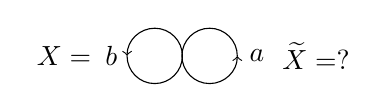
\begin{tikzpicture}
    \node at (-1.20,0) {$X=$};
    \draw [<-] (1,0) arc (360:0:10pt);
    \node at (1.25,0) {$a$};
    \draw [<-] (-0.40,0) arc (180:-180:10pt);
    \node at (-0.60,0) {$b$};
    \node at (2,0) {$\widetilde{X}=$?};
  \end{tikzpicture}

  $\widetilde{X}$ è rappresentato dal seguente grafo, con $\tilde{a}$ rappresentato dalle frecce orizzontali dirette verso destra (e $\tilde{a}^{-1}$ verso sinistra) e $\tilde{b}$ da quelle verticali verso l'alto (e $\tilde{b}^{-1}$ verso il basso):
  \begin{center}
    \begin{tikzpicture}
      \draw l-system [l-system={cayley, axiom=[A] [+A] [++A] [-A], step=1cm, order=3}];
      \node at (0.5,-0.15) {$\tilde{a}$};
      \node at (0.15,0.5) {$\tilde{b}$};
    \end{tikzpicture}
  \end{center}
  È un albero quadrivalente infinito. I segmenti orizzontali si proiettano su $a$, quelli verticali su $b$. Chi è il rivestimendo di $X$ associato ad $H=\langle a \rangle$? Cerchiamo un rivestimento $E \xrightarrow[]{p} X$ con $p_{\star}(\pi_1(E, \tilde{x}))=\langle a \rangle$. Il grafo è il seguente:
  \begin{center}
    \begin{tikzpicture}
      \draw l-system [l-system={cayley, axiom=[+A] [-A], step=1cm, order=3}];
      \draw [->] (0.7,0) arc (360:0:10pt);
      \node at (0.95,0) {$a$};
      \node at (-0.3,0) {$\tilde{x}_0$};
      \filldraw (0,0) circle (1pt);
    \end{tikzpicture}
  \end{center}
  Non è omogeneo: se $\varphi:E \rightarrow E$ è un omeomorfismo, $\varphi(\text{loop})=\text{loop} \implies \varphi(\tilde{x}_0)=\tilde{x}_0 \implies \text{Aut}(E)=\{1\}$. In effetti $\langle a \rangle$ è molto lontano dall'essere normale in $\pi_1(X, x)=\mathbb{Z} * \mathbb{Z}$.
  Se $N(a)$ è il sottogruppo normale generato da $a$ in $\pi_1(X)$, il rivestimento associato a $N$ come sarà fatto?
  $N$ normale $\implies$ il rivestimento associato $E \xrightarrow[]{p} X$ sarà regolare e $\text{Aut}(E)=\faktor{\pi_1(X, x)}{p_{\star}(\pi_1(E, \tilde{x}))}=\faktor{\mathbb{Z} * \mathbb{Z}}{N}=\langle a, b \mid a \rangle \overset{\psi}{\cong} \mathbb{Z}$,
  \begin{align*}
    \psi:\mathbb{Z}*\mathbb{Z} &\longrightarrow \mathbb{Z} \\
    a &\longmapsto 0 \\
    b &\longmapsto 1
  \end{align*}
  induce l'isomorfismo. Ecco $E$:
  \begin{center}
    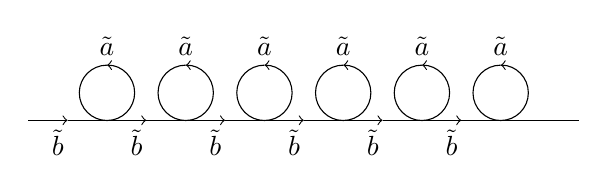
\begin{tikzpicture}
      \draw[->] (0,0) -- node[below, near end]{$\tilde{b}$} (0.5,0);
      \draw (0.5,0) -- (1,0);
      \draw [<-] (1,0.7) arc (450:90:10pt) node[above]{$\tilde{a}$};
      \draw[->] (1,0) -- node[below, near end]{$\tilde{b}$} (1.5,0);
      \draw (1.5,0) -- (2,0);
      \draw [<-] (2,0.7) arc (450:90:10pt) node[above]{$\tilde{a}$};
      \draw[->] (2,0) -- node[below, near end]{$\tilde{b}$} (2.5,0);
      \draw (2.5,0) -- (3,0);
      \draw [<-] (3,0.7) arc (450:90:10pt) node[above]{$\tilde{a}$};
      \draw[->] (3,0) -- node[below, near end]{$\tilde{b}$} (3.5,0);
      \draw (3.5,0) -- (4,0);
      \draw [<-] (4,0.7) arc (450:90:10pt) node[above]{$\tilde{a}$};
      \draw[->] (4,0) -- node[below, near end]{$\tilde{b}$} (4.5,0);
      \draw (4.5,0) -- (5,0);
      \draw [<-] (5,0.7) arc (450:90:10pt) node[above]{$\tilde{a}$};
      \draw[->] (5,0) -- node[below, near end]{$\tilde{b}$} (5.5,0);
      \draw (5.5,0) -- (6,0);
      \draw [<-] (6,0.7) arc (450:90:10pt) node[above]{$\tilde{a}$};
      \draw (6,0) -- (6.5,0);
      \draw (6.5,0) -- (7,0);
    \end{tikzpicture}
  \end{center}
\end{ex}


\subsection{$\pi_1$ di grafi finiti (connessi)}
Sia $\Gamma$ un grafo finito connesso con $V$ vertici e $E$ lati. Diciamo che $\Gamma$ è un albero se non contiene cicli, cioè loop iniettivi.

\begin{ftt}
  \begin{nlist}
    \item Un albero è contraibile (per induzione sul numero di vertici).
    \item Se $\Gamma$ è un albero, $V-E=1$ (induzione).
    \item $\Gamma$ connesso $\implies$ $\Gamma$ contiene un albero massimale $\Gamma'$ e $\Gamma'$ contiene tutti i vertici di $\Gamma$ $\implies$ $\Gamma=\Gamma'\cup\{\text{qualche lato}\}$.
    \item Definiamo $\chi(\Gamma)=\text{caratteristica di Eulero di }\Gamma=V-E$. Se $\Gamma' \subseteq \Gamma$ ($\Gamma$ connesso) è un albero massimale, $\chi(\Gamma')=1$ $\implies$ $\Gamma=\Gamma'\cup\{(1-\chi(\Gamma))\text{ lati}\}$.
    \item Dunque $\Gamma$ è ottenuto da un albero massimale aggiungendo $1-\chi(\Gamma)$ lati. Usando induttivamente Van Kampen, otteniamo il seguente teorema, di cui omettiamo la dimostrazione.
  \end{nlist}
\end{ftt}

\begin{thm}
  $\pi_1(\Gamma) \cong F_{1-\chi(\Gamma)}$, il gruppo libero su $1-\chi(\Gamma)$ generatori.
\end{thm}

\begin{thm}
  Sia $F$ il gruppo libero su $n$ generatori, $H<F$ sottogruppo di indice $k$. Allora $H$ è un gruppo libero su $k(n-1)+1$ generatori (in particolare, il rango di $H$ è spesso maggiore di quello di $F$).
\end{thm}

\begin{proof}
  $F=\pi_1(\Gamma), \chi(\Gamma)=1-n$ per il teorema appena visto. Sia $\widetilde{\Gamma}$ il rivestimento di $\Gamma$ associato ad $H$.
  Poiché vertici e lati sono semplicemente connessi, se $V, E$ sono vertici e lati di $\widetilde{\Gamma}$, allora i vertici e lati di $\widetilde{\Gamma}$ sono $k \cdot V, k \cdot E$, in quanto $\deg{(\text{rivestimento})}=[F:H]=k \implies H=\pi_1(\widetilde{\Gamma})=F_{1-\chi(\widetilde{\Gamma})}=F_{1-k\chi(\Gamma)}=F_{1-k(1-n)}=F_{k(n-1)+1}$.
\end{proof}


\newpage

\section{Analisi complessa}

\subsection{Funzioni olomorfe}
Adesso studiamo le funzioni complesse.

Sia $U \subset \mathbb{C}$ aperto, $f:U \longrightarrow \mathbb{C}$. Possiamo scrivere $f(z)=u(z)+iv(z)$ per ogni $z \in U$. Chiamiamo $u(z)$ la parte reale di $f$, $u:U \longrightarrow \mathbb{R}$, $v(z)$ la parte immaginaria di $f$, $v:U \longrightarrow \mathbb{R}$.

\begin{ftt}
  $f:U \longrightarrow \mathbb{C}$ è continua in $z_0 \in U$ (rispettivamente in tutto $U$) se e solo se $u$ e $v$ sono continue in $z_0 \in U$ (rispettivamente in tutto $U$).
\end{ftt}

Importante: dal punto di vista della continuità le funzioni di $U$ a valori complessi possono essere semplicemente viste come funzioni da $U \subseteq \mathbb{R}^2$ a valori reali. Domanda: vale la stessa cosa quando parliamo di derivabilità?

\begin{defn}
  (Differenziabilità) La funzione $f:U \longrightarrow \mathbb{C}$ è \textit{differenziabile in $z_0 \in U$} se esiste $A:\mathbb{C} \longrightarrow \mathbb{C}$ applicazione $\mathbb{R}$-lineare t.c.
  \begin{nlist}
    \item $f(z)=f(z_0)+A(z-z_0)+r(z)$;
    \item $\dfrac{|r(z)|}{|z-z_0|} \xrightarrow[]{z \longrightarrow z_0} 0$.
  \end{nlist}
  In questo caso, chiamiamo l'applicazione $A$ \textit{jacobiano di $f$}, $A=: Jf_{z_0}$.
\end{defn}

\begin{oss}
  $f$ differenziabile in $z_0$ $\implies$ $f$ continua in $z_0$.
\end{oss}

Fissiamo la base $\{1, i\}$ di $\mathbb{C}$ come $\mathbb{R}$-spazio vettoriale.
\begin{align*}
  f:U &\longrightarrow \mathbb{C}\\
  z=x+iy &\longmapsto u(x, y)+iv(x, y)
\end{align*}

\begin{ftt}
  \begin{nlist}
    \item Se $f$ è differenziabile in $x_0+iy_0=z_0 \in U$, esistono le derivate parziali di $f$ in $z_0$ e $Jf_{z_0}=\begin{pmatrix}
      \dfrac{\partial u}{\partial x}(x_0, y_0) & \dfrac{\partial u}{\partial y}(x_0, y_0)\\
      \dfrac{\partial v}{\partial x}(x_0, y_0) & \dfrac{\partial v}{\partial y}(x_0, y_0)
  \end{pmatrix}$;
  \item (teorema del differenziale totale): se esistono $\dfrac{\partial u}{\partial x}, \dfrac{\partial u}{\partial y}, \dfrac{\partial v}{\partial x}, \dfrac{\partial v}{\partial y}$ in un intorno di $z_0$ e sono continue in $z_0$, allora $f$ è differenziabile in $z_0$.
  \end{nlist}
\end{ftt}

\begin{exc}
  \begin{align*}
    f:\mathbb{R}^2 &\longrightarrow \mathbb{R}\\
    (x, y) &\longmapsto \begin{cases} x & \mbox{se }y\not=x^2 \\ 0 & \mbox{se }y=x^2 \end{cases}
  \end{align*}
  è differenziabile in $(0, 0)$?
\end{exc}

\begin{defn}
  (Funzione olomorfa) Siano $U \subseteq \mathbb{C}$ aperto, $f:U \longrightarrow \mathbb{C}$ continua. Diciamo che $f$ è \textsc{olomorfa in $z_0 \in \mathbb{C}$} se esiste $\displaystyle \lim_{\substack{h \longrightarrow 0 \\ h\not=0}} \frac{f(z_0+h)-f(z_0)}{h}$. Se tale limite esiste, lo chiamiamo derivata di $f$ in $z_0$ e lo denotiamo con $f'(z_0)$.
  Diciamo che $f$ è \textsc{olomorfa in $U$} se è olomorfa per ogni $z_0 \in U$. Diciamo che $f$ è \textsc{intera} se è definita su tutto $\mathbb{C}$ ed è olomorfa in $\mathbb{C}$.
\end{defn}

\begin{prop}
  Sia $U \subset \mathbb{C}$ aperto, $f, g:U \longrightarrow \mathbb{C}$ olomorfe in $z_0 \in U$.
  \begin{nlist}
    \item $f+g$ è olomorfa in $z_0$ e $(f+g)'(z_0)=f'(z_0)+g'(z_0)$;
    \item $f \cdot g$ è olomorfa in $z_0$ e $(f \cdot g)'(z_0)=f'(z_0)g(z_0)+f(z_0)g'(z_0)$;
    \item se $g(z_0) \not=0$, $\dfrac{f}{g}$ è olomorfa in $z_0$ e $\left(\dfrac{f}{g}\right)9(z_0)=\dfrac{f'(z_0)g(z_0)-f(z_0)g'(z_0)}{g(z_0)^2}$.
  \end{nlist}
\end{prop}

\begin{prop}
  Siano $U, V$ aperti di $\mathbb{C}$, $f:U \longrightarrow V$, $g:V \longrightarrow \mathbb{C}$, $f$ olomorfa in $z_0 \in U$ è $g$ olomorfa in $f(z_0)$. Allora $g \circ f$ è olomorfa in $z_0$ e $(g \circ f)'(z_0)=g'(f(z_0))\cdot f'(z_0)$.
\end{prop}

\begin{ex}
  \begin{nlist}
    \item $f(z)=z$ è una funzione intera. Infatti, $\dfrac{f(z+h)-f(z)}{h}=\dfrac{z+h-z}{h}=1$ $\implies$ $f$ è olomorfa in $z \in \mathbb{C}$ e $f'(z)=1$;
    \item $f(z)=z^n, n \ge 1$ è intera.
    Infatti, $\displaystyle \frac{f(z+h)-f(z)}{h}=\frac{(z+h)^n-z^n}{h}=\frac{\sum_{k=0}^n \binom{n}{k}z^kh^{n-k}-z^n}{h}=\sum_{k=0}^{n-1} \binom{n}{k}z^kh^{n-k-1} \xrightarrow[\substack{h \longrightarrow 0 \\ h\not=0}]{} \binom{n}{n-1} z^{n-1}=$\\
    $=nz^{n-1}=:f'(z)$.
  \end{nlist}
\end{ex}

\begin{exc}
  Provare che $f(z)=z^n, n<0$ è olomorfa in $\mathbb{C}\setminus\{0\}$.
\end{exc}

\begin{oss}
  I polinomi sono funzioni intere. Le funzioni razionali $\dfrac{P(z)}{Q(z)}$ con $P$ e $Q$ polinomi sono olomorfe in $\mathbb{C} \setminus \{z \in \mathbb{C} \mid Q(z)=0\}$.
\end{oss}

\begin{ex}
  (Una funzione non olomorfa) $f(z)=\bar{z}$ non è olomorfa. $\dfrac{f(z+h)-f(z)}{h}=\dfrac{\bar{z}+\bar{h}-\bar{z}}{h}=\dfrac{\bar{h}}{h}$ per $h \in \mathbb{C}, h \not=0$. Se esiste $f'(z)$, allora il limite dovrebbe esistere per ogni possibile direzione per cui $h \longrightarrow 0, h\not=0$. Se esiste $f'(z)$, dobbiamo per esempio avere che
  \begin{align*}
    1=\lim_{\substack{h \longrightarrow 0 \\ h\not=0 \\ \mathfrak{Im}(h)=0}} \frac{\bar{h}}{h}=\lim_{\substack{h \longrightarrow 0 \\ h\not=0 \\ \mathfrak{Im}(h)=0}} \frac{f(z+h)-f(z)}{h}=\\
    =\lim_{\substack{h \longrightarrow 0 \\ h\not=0 \\ \mathfrak{Re}(h)=0}} \frac{f(z+h)-f(z)}{h}=\lim_{\substack{h \longrightarrow 0 \\ h\not=0 \\ \mathfrak{Re}(h)=0}} \frac{\bar{h}}{h}=-1,
  \end{align*}
  assurdo $\implies$ non può esistere $f'(z)$.
\end{ex}

Domanda: qual è il legame tra l'olomorficità di $f:U \longrightarrow \mathbb{C}$ e la differenziabilità di $f$ vista come funzione da $U \subset \mathbb{R}^2$ in $\mathbb{R}^2$?

\begin{oss}
  Come nel caso della differenziabilità in ambito reale, $f$ olomorfa in $z_0$ $\implies$ $f$ continua in $z_0$. Infatti, $f(z)-f(z_0)=\dfrac{f(z)-f(z_0)}{z-z_0}(z-z_0)$; al limite per $z \longrightarrow z_0$, abbiamo che tende  $\displaystyle f'(z_0) \cdot \lim_{z \longrightarrow z_0} (z-z_0)=f'(z_0) \cdot 0=0$.
\end{oss}

\begin{ex}
  $g(z)=\bar{z}$ non è olomorfa ma nella base $\{1, i\}$ di $\mathbb{C}$
  \begin{align*}
    g: \mathbb{R}^2 &\longrightarrow \mathbb{R}^2\\
    (x, y) &\longmapsto (x, -y)
  \end{align*}
   è differenziabile.
\end{ex}

\begin{thm} \label{car_olo}
  Sia $U \subset \mathbb{C}$ un aperto e $f:U \longrightarrow \mathbb{C}$ continua. $f$ è olomorfa in $z_0 \in U$ $\iff$ le seguenti due condizioni sono soddisfatte:
  \begin{nlist}
    \item $f$ è differenziabile in $z_0$;
    \item $Jf_{z_0}:\mathbb{C} \longrightarrow \mathbb{C}$ corrisponde alla moltiplicazione per $a \in \mathbb{C}$.
  \end{nlist}
\end{thm}

\begin{proof}
  ($\implies$) \\ L'olomorficità implica che $f(z_0+h)=f(z_0)+f'(z_0)h+r(h) \, (\star)$ con \\ $\dfrac{|r(h)|}{|h|} \xrightarrow[h \longrightarrow 0, h \not=0]{} 0$.
  Nella base $\{1, i\}$ di $\mathbb{C}$, possiamo riscrivere l'equazione $(\star)$ come ($z_0=x_0+iy_0, h=\alpha+i\beta$) $f(x_0+\alpha, y_0+\beta)=f(x_0, y_0)+f'(z_0)(\alpha+i\beta)+r(\alpha, \beta)$ con $\dfrac{|r(\alpha, \beta)|}{\sqrt{\alpha^2+\beta^2}} \longrightarrow 0$.
  La mappa
  \begin{align*}
    \mathbb{C} &\longrightarrow \mathbb{C}\\
    z &\longmapsto az,
  \end{align*}
  $a:=f'(z_0)$ è $\mathbb{R}$-lineare $\implies$ $f$ differenziabile in $z_0$ e $Jf_{z_0}=\text{moltiplicazione per }a=f'(z_0)$.

  ($\Leftarrow$) La dimostrazione è analoga:
  \begin{enumerate}
    \item si parte dalla definizione di differenziabilità nelle variabili $x, y$;
    \item si riscrive in termini di $z$;
    \item si usa che $Jf_{z_0}=\text{moltiplicazione per }a \in \mathbb{C} \implies f'(z_0)=a$.
  \end{enumerate}
\end{proof}

Obiettivo: sostituire la condizione (ii) con le cosiddette condizioni di Cauchy-Riemann.

\begin{lm} \label{c-lineare}
  Sia $A: \mathbb{C} \longrightarrow \mathbb{C}$ $\mathbb{R}$-lineare. Le seguenti affermazioni sono equivalenti:
  \begin{nlist}
    \item $A$ è indotta dalla moltiplicazione per un numero complesso, cioè $A(z)=a \cdot z$ per un certo $a \in \mathbb{C}$;
    \item $A$ è $\mathbb{C}$-lineare;
    \item $A(i)=iA(1)$;
    \item $A=\text{moltiplicazione per la matrice }\begin{pmatrix}
      \alpha & -\beta\\
      \beta & \alpha
  \end{pmatrix}$ dove $\alpha, \beta \in \mathbb{R}$ (nella base $\{1, i\}$ di $\mathbb{C}$).
  \end{nlist}
\end{lm}

\begin{proof}
  Per esercizio.
\end{proof}

\begin{oss}
  $a=\alpha+i\beta$.
\end{oss}

\begin{thm}
  (Cauchy-Riemann) Sia $U \subset \mathbb{C}$ aperto, $f:U \longrightarrow \mathbb{C}$ continua. $f(x, y)=u(x, y)+iv(x, y)$ nella base $\{1, i\}$ di $\mathbb{C}$. $f$ è olomorfa in $z_0 \in U$ $\iff$ valgono le seguenti:
  \begin{nlist}
    \item $f$ è differenziabile in $z_0$;
    \item valgono le \textsc{condizioni di Cauchy-Riemann}: $\dfrac{\partial u}{\partial x}(x_0, y_0)=\dfrac{\partial v}{\partial y}(x_0, y_0)$ e $\dfrac{\partial u}{\partial y}(x_0, y_0)=-\dfrac{\partial v}{\partial x}(x_0, y_0)$.
  \end{nlist}
  Nel caso $f$ sia olomorfa, $f'(z_0)=\dfrac{\partial u}{\partial x}(z_0)+i\dfrac{\partial v}{\partial x}(z_0)=$espressioni equivalenti usando le condizioni di Cauchy-Riemann.
\end{thm}

\begin{proof}
  Dobbiamo semplicemente provare che (ii) del teorema \ref{car_olo} equivale a (ii) di questo teorema. $Jf_{z_0}=\begin{pmatrix}
    \frac{\partial u}{\partial x}(z_0) & \frac{\partial u}{\partial y}(z_0)\\
    \frac{\partial v}{\partial x}(z_0) & \frac{\partial v}{\partial y}(z_0)
\end{pmatrix}$ che, per il punto (ii) del teorema \ref{car_olo}, equivale alla moltiplicazione per $a \in \mathbb{C}$, che per il lemma \ref{c-lineare} corrisponde all'applicazione lineare data dalla matrice $\begin{pmatrix}
  \alpha & -\beta\\
  \beta & \alpha
\end{pmatrix}$. Imponendo l'uguaglianza troviamo le condizioni di Cauchy-Riemann.
\end{proof}

\begin{defn}
  $z=x+iy, e^z:=e^x(\cos{y}+i\sin{y})$.
\end{defn}

\begin{prop}
  $f(z)=e^z$ è intera con $f'(z)=e^z$.
\end{prop}

\begin{proof}
  Nella base $\{1, i\}$ di $\mathbb{C}$ scriviamo $f(x, y)=u(x, y)+iv(x, y)$, $u(x, y)=e^x\cos{y}, v(x, y)=e^x\sin{y}$.
  \begin{enumerate}
    \item $f$ è differenziabile: ovvio.
    \item Verifichiamo le condizioni di C-R:
    $\dfrac{\partial u}{\partial x}=e^x\cos{y}, \dfrac{\partial u}{\partial y}=-e^x\sin{y}, \dfrac{\partial v}{\partial x}=e^x\sin{y}, \dfrac{\partial v}{\partial y}=e^x\cos{y} \implies f(z)$ soddisfa C-R e $f'(z)=e^z$.
  \end{enumerate}
\end{proof}

\begin{ex}
  Altri esempi di funzioni intere:
  $$\sin{z}:=\dfrac{e^{iz}-e^{-iz}}{2i}, \cos{z}:=\dfrac{e^{iz}+e^{-iz}}{2}, \sinh{z}:=\dfrac{e^{z}-e^{-z}}{2}, \cosh{z}:=\dfrac{e^{z}+e^{-z}}{2}.$$
\end{ex}

\begin{cor}
  Sia $f:U \longrightarrow \mathbb{C}$ olomorfa con $U \subset \mathbb{C}$ aperto connesso. Le seguenti affermazioni sono equivalenti:
  \begin{nlist}
    \item $f$ è costante in $U$;
    \item $f'$ è identicamente nulla;
    \item $\mathfrak{Re}(f)$ è costante in $U$;
    \item $\mathfrak{Im}(f)$ è costante in $U$.
  \end{nlist}
\end{cor}

\begin{proof}
  (i) $\implies$ (iii) e (i) $\implies$ (iv) sono ovvie. Adesso vogliamo usare il teorema di Cauchy-Riemann per la caratterizzazione delle funzioni olomorfe.

  (i) $\iff$ (ii) $f$ è costante in $U$ $\iff$ $Jf$ è identicamente nullo, ma $Jf$ era la moltiplicazione per la matrice $\begin{pmatrix}
    \alpha & -\beta\\
    \beta & \alpha
\end{pmatrix}$ dove $f'(z)=\alpha+i\beta$, quindi $Jf \equiv 0 \iff \alpha =\beta=0 \iff f'(z)=0$.

(iii) $\implies$ (i) e (iv) $\implies$ (i) Adesso bisogna usare C-R. Nella base $\{1, i\}$ di $\mathbb{C}$, scriviamo $f(x, y)=u(x, y)+iv(x, y)$.
$\mathfrak{Re}(f)$ costante $\iff$ $u$ costante $\iff$ $\dfrac{\partial u}{\partial x}=0=\dfrac{\partial u}{\partial y}$ e per C-R abbiamo $\dfrac{\partial v}{\partial x}=0=\dfrac{\partial v}{\partial y}$. (iv) $\implies$ (i) è analogo.
\end{proof}


\subsection{Serie}
Vediamo ora, senza dimostrazione, alcuni risultati sulle serie di numeri complessi che ci torneranno utili.

\begin{defn}
  Sia $(c_n)_{n \in \mathbb{N}}$ una successione di numeri complessi. Diciamo che $\displaystyle \sum_{n \ge 0} c_n$ è \textit{assolutamente convergente} se la serie $\displaystyle \sum_{n \ge 0} |c_n|$ è convergente.
\end{defn}

\begin{exc}
  $\displaystyle \sum_{n \ge 0} \frac{i^n}{n!}$ è convergente?
\end{exc}

\begin{prop} \label{sum&prod}
  Siano $\displaystyle \sum_{n \ge 0} a_n$ e $\displaystyle \sum_{n \ge 0} b_n$ due serie assolutamente convergenti.
  \begin{nlist}
    \item $\displaystyle \sum_{n \ge 0} a_n+b_n$ è assolutamente convergente ed è uguale a $\displaystyle \sum_{n \ge 0} a_n + \sum_{n \ge 0} b_n$ (la serie delle somme è la somma delle serie);
    \item se $\displaystyle c_n:=\sum_{p=0}^n a_pb_{n-p}$, allora $\displaystyle \sum_{n \ge 0} c_n$ è assolutamente convergente e la sua somma è uguale al prodotto delle somme delle due serie date.
  \end{nlist}
\end{prop}

\begin{defn}
  Sia $\displaystyle \sum_{n \ge 0} a_nz^n$ una serie di potenze. Chiamiamo \textit{raggio di convergenza} la quantità $\displaystyle \rho:=\sup\{r \in \mathbb{R}, r>0 \mid \sum_{n \ge 0} |a_n|r^n \text{ è convergente}\}$.
\end{defn}

\begin{oss}
  $\rho$ può essere finito e in questo caso $\rho \ge 0$, oppure $\rho=+\infty$.
\end{oss}

\begin{defn}
  Chiamiamo \textit{disco di convergenza} l'insieme $\{z \in \mathbb{C} \mid |z|<\rho\}$.
\end{defn}

\begin{oss}
  Il disco di convergenza è aperto e $\rho=0$ $\implies$ disco$=\emptyset$.
\end{oss}

\begin{prop}
  Data una serie di potenze $\displaystyle \sum_{n \ge 0} a_nz^n$, esiste $0 \le \rho \le +\infty$ t.c.:
  \begin{enumerate}
    \item caso $\rho=0$ la serie converge solo per $z=0$;
    \item caso $\rho=+\infty$: la serie converge assolutamente per ogni $z \in \mathbb{C}$;
    \item caso $0<\rho<+\infty$: se $|z|<\rho$ la serie converge assolutamente, se $|z|>\rho$ la serie non converge.
  \end{enumerate}
  Inoltre si ha la formula di Hadamard:
  $$\frac{1}{\rho}=\limsup_{n \longrightarrow +\infty} |a_n|^{1/n}$$
  con la convenzione che $\rho=+\infty$ se il limite è $0$ e $\rho=0$ se il limite è $+\infty$.
\end{prop}

\begin{exc}
  Calcolare il raggio di convergenza di \\
  $\displaystyle \sum_{n \ge 0} n!z^n, \sum_{n \ge 0} \frac{z^n}{n!}, \sum_{n \ge 0} (-1)^n \frac{z^{2n}}{(2n)!}, \sum_{n \ge 0} (-1)^n \frac{z^{2n+1}}{(2n+1)!}$.
\end{exc}

\begin{ex}
  Proviamo che $\displaystyle \sum_{n \ge 0} z^n=\frac{1}{1-z}$ per $|z|<1$. La somma della serie è $\displaystyle \lim_{n \longrightarrow +\infty}S_n, S_n=z^0+z^1+\dots+z^n=\frac{1-z^{n+1}}{1-z}$. Lo studio del limite è lasciato per esercizio.
\end{ex}

\begin{ftt}
  \begin{nlist}
    \item Siano $\displaystyle \sum_{n \ge 0} a_nz^n$ e $\displaystyle \sum_{n \ge 0} b_nz^n$ due serie di potenze con raggio di convergenza $\ge R$ per qualche $R$.
    Allora, definendo $\displaystyle S(z):=\sum_{n \ge 0} a_nz^n+\sum_{n \ge 0}b_nz^n, P(z):=\left(\sum_{n \ge 0}a_nz^n\right)\left(\sum_{n \ge 0}b_nz^n\right)$, abbiamo che $S(z)$ e $P(z)$ hanno raggio di convergenza $\ge R$.
    Inoltre, per ogni $r \in \mathbb{C}$ con $|r|<R$, $\displaystyle S(r)=\sum_{n \ge 0}a_nr^n+\sum_{n \ge 0} b_nr^n$ e $\displaystyle P(r)=\left(\sum_{n \ge 0}a_nr^n\right)\left(\sum_{n \ge 0}b_nr^n\right)$.
    \item Sia $\displaystyle f(z)=\sum_{n \ge 0} a_nz^n$. Chiamiamo \textit{serie derivata} la serie di potenze $\displaystyle \sum_{n \ge 0} na_nz^{n-1}$ e la denotiamo con $f'(z)$. Allora $f$ e $f'$ hanno lo stesso raggio di convergenza.
  \end{nlist}
\end{ftt}

Passiamo ora a definire alcune funzioni complesse tramite serie di potenze. Cominciamo da esponenziale, seno e coseno.

\begin{defn}
  Fissato $z \in \mathbb{C}$, chiamiamo \textit{esponenziale del numero complesso $z$} la quantità $\displaystyle e^z:=\sum_{n \ge 0} \frac{1}{n!}z^n$.
  Chiamiamo \textit{coseno di $z$} $\displaystyle \cos{z}:=\sum_{n \ge 0}(-1)^n\frac{z^{2n}}{(2n)!}$ e \textit{seno di $z$} $\displaystyle \sum_{n \ge 0}(-1)^n \frac{z^{2n+1}}{(2n+1)!}$.
\end{defn}

\begin{oss}
  Le definizioni sono ben poste perché le serie hanno raggio di convergenza infinito.
\end{oss}

\begin{exc}
  Provare che le definizioni coincidono con quelle già date.
\end{exc}

\begin{ex}
  Dati $z, z' \in \mathbb{C}$, $e^{z+z'}=e^ze^{z'}$. Siano $a_n=\dfrac{1}{n!}z^n, b_n=\dfrac{1}{n!}(z')^n$.
  Sia $\displaystyle c_n=\sum_{p=0}^n a_pb_{n-p}=\sum_{p=0}^n \left(\frac{1}{p!}z^p\right)\left(\frac{1}{(n-p)!}(z')^{n-p}\right)=\frac{1}{n!}\sum_{p=0}^n\binom{n}{p}z^p(z')^{n-p}=\frac{1}{n!}(z+z')^n$,
  allora per il punto (ii) della proposizione \ref{sum&prod} abbiamo proprio $e^{z+z'}=e^ze^{z'}$.
\end{ex}

Adesso vogliamo definire il logaritmo.

\begin{defn}
  Sia $z \in \mathbb{C}, z \not=0$. Chiamiamo \textit{logaritmo del numero complesso $z$} la quantità $\log{z}:=\log{|z|}+i\arg{z}$.
\end{defn}

\begin{oss}
  $\log{z} \in \mathbb{C}$ è definito modulo $2\pi i \mathbb{Z}$ perché $\arg{z} \in \faktor{\mathbb{R}}{2\pi \mathbb{Z}}$.
\end{oss}

\begin{prop}
  Per ogni $z \in \mathbb{C}, z \not=0$, $e^{\log{z}}=z$.
\end{prop}

\begin{ftt}
  $\log{(zz')}=\log{z}+\log{z'} \mod{2\pi i \mathbb{Z}}$.
\end{ftt}

Domanda: come definiamo $z \longmapsto \log{z}$? Abbiamo bisogno della definizione di branca.

\begin{defn}
  Sia $D$ aperto connesso di $\mathbb{C}$ t.c. $0 \not\in D$ e $f:D \longrightarrow \mathbb{C}$ continua. Diciamo che $f$ è una \textit{branca} di $\log{z}$ se $e^{f(z)}=z$ (cioè se $f(z)$ è uno dei possibili valori di $\log{z}$).
\end{defn}

\begin{prop}
  Assumiamo che esista una branca $f(z)$ di $\log{z}$ in $D$. Allora ogni altra branca di $\log{z}$ in $D$ è della forma $f(z)+k(2\pi i)$ per qualche intero $k$. Viceversa, $f(z)+k(2 \pi i)$ è una branca di $\log{z}$ per ogni intero $k$, a partire dalla branca fissata $f(z)$.
\end{prop}

\begin{proof}
  Siano $f(z)$ e $g(z)$ due branche di $\log{z}$ in $D$ ($e^{f(z)}=z, e^{g(z)}=z$ per ogni $z \in D$). $h(z):=\dfrac{1}{2\pi i}(g(z)-f(z)):D \longrightarrow \mathbb{C}$. $h$ è continua e t.c. $\Ima{h} \subseteq \mathbb{Z}$.
  Visto che $D$ è connesso, $h$ è costantemente uguale a un certo intero $k$ $\implies$ $g(z)=f(z)+k(2\pi i)$. Il viceversa è ovvio.
\end{proof}

\begin{oss}
  \begin{nlist}
    \item Possiamo dare una definizione di branca anche per $\arg{z}$;
    \item ogni branca di $\arg{z}$ definisce una branca di $\log{z}$ (e viceversa) (se $f(z)$ è una branca di $\arg{z}$, $\log{|z|}+if(z)$ è una branca di $\log{z}$).
  \end{nlist}
\end{oss}

\begin{oss}
  Sia $D=\{z \in \mathbb{C} \mid \mathfrak{Re}(z)>0\}$. Per ogni $z \in D$ esiste un unico $-\pi/2<\phi<\pi/2$ t.c. $\phi$ è un argomento di $z$; poniamo allora $\text{Arg}(z):=\phi$.
\end{oss}

\begin{prop}
  La funzione
  \begin{align*}
    \text{Arg}(z):D &\longrightarrow \mathbb{C}\\
    z &\longmapsto \phi
  \end{align*}
  è continua.
\end{prop}

\begin{proof}
  Non l'ha ancora fatta, verrà aggiunta asap.
\end{proof}

\begin{defn}
  Chiamiamo branca \textit{principale} di $\log{z}$ la funzione continua $\log{z}+i\text{Arg}(z)$ per $z \in D=\{z \in \mathbb{C} \mid \mathfrak{Re}(z)>0\}$.
\end{defn}


\subsection{Funzioni analitiche}
\begin{defn}
  (Funzione analitica) Sia $U \subset \mathbb{C}$ un aperto. Una funzione $f:U \longrightarrow \mathbb{C}$ si dice \textsc{analitica in $z_0 \in U$} se
  \begin{nlist}
    \item esiste una serie di potenze $\displaystyle \sum_{n \ge 0} a_n(z-z_0)^n$ che converge assolutamente per $|z-z_0|<r$ per un qualche $r>0$ e
    \item $\displaystyle f(z)=\sum_{n \ge 0} a_n(z-z_0)^n$ per $|z-z_0|<r$.
  \end{nlist}
  Diremo che $f$ è \textsc{analitica in $U$} se $f$ è analitica in $z_0$ per ogni $z_0 \in U$.
\end{defn}

\begin{oss}
  $\displaystyle \sum_{n \ge 0} a_n(z-z_0)^n=a_0+\sum_{n \ge 1} a_n(z-z_0)^n$.
\end{oss}

\begin{ex}
  Sono funzioni analitiche:
  \begin{nlist}
    \item i polinomi;
    \item $e^z, \cos{z}, \sin{z}, \dots$
  \end{nlist}
\end{ex}

\begin{prop}
  Sia $U \subset \mathbb{C}$ un aperto e siano $f, g:U \longrightarrow \mathbb{C}$ funzioni analitiche in $U$. Allora
  \begin{nlist}
    \item $f+g$ è analitca in $U$;
    \item $fg$ è analitica in $U$;
    \item $\dfrac{f}{g}$ è definita e analitica in qualunque aperto contenuto in $\{z \in U \mid g(z) \not=0\}$.
  \end{nlist}
\end{prop}

\begin{prop}
  Siano $U$ e $V$ aperti di $\mathbb{C}$. Siano $f:U \longrightarrow V$ e $g:V \longrightarrow \mathbb{C}$ funzioni analitiche. Allora $g \circ f$ è analitica in $U$.
\end{prop}

\begin{prop}
  Sia $U \subset \mathbb{C}$ aperto e $f:U \longrightarrow \mathbb{C}$ una funzione. Se $f$ è analitica in $U$, allora $f$ è continua in $U$.
\end{prop}

\begin{proof}
  Sia $z_0 \in U$. Assumiamo che $\displaystyle f(z)=\sum_{n \ge 0}(z-z_0)^n$ per $|z-z_0|<r$ per qualche $r>0$. Senza perdita di generalità $z_0=0$ e $f(z_0)=f(0)=0$ $\implies$ $a_0=f(z_0)=f(0)=0$.
  $\displaystyle f(z)=\sum_{n \ge 0} a_n(z-z_0)^n=\sum_{n \ge 0} a_nz^n=\sum_{n \ge 1} a_nz^n=z\sum_{n \ge 1} a_nz^{n-1}$. Se $0<\rho<r$ e $|z|<\rho$, $\displaystyle |f(z)| \le \sum_{n \ge 1} |a_n||z^n| \le |z| \sum_{n \ge 1} |a_n||z|^{n-1} \le |z| \sum_{n \ge 1} |a_n| \rho^{n-1}$.
  Adesso notiamo che $\displaystyle \sum_{n \ge 1} |a_n| \rho^{n-1}$ non dipende da $|z|$, quindi $|f(z)| \longrightarrow 0$ per $|z| \longrightarrow 0$.
\end{proof}

\begin{prop}
  Sia $z_0 \in \mathbb{C}$. Sia $\displaystyle \sum_{n \ge 0} a_n(z-z_0)^n$ una serie di potenze assolutamente convergente nel disco aperto $D_r(z_0)=\{z \mid |z-z_0|<r\}$ per qualche $r>0$. Allora la funzione
  \begin{align*}
    f:D_r(z_0) &\longrightarrow \mathbb{C}\\
    z &\longmapsto \sum_{n \ge 0} a_n(z-z_0)^n
  \end{align*}
  è analitica in $D_r(z_0)$.
\end{prop}

\begin{proof}
  Senza perdita di generalità $z_0=0$ $\implies$ $\displaystyle f(z)=\sum_{n \ge 0} a_nz^n$. Sia $a \in D_r(0)$ e sia $s \in \mathbb{R}, s>0$ t.c. $|a|+s<r$. Notiamo che $\displaystyle z^n=((z-a)+a)^n=\displaystyle \sum_{0 \le k \le n} \binom{n}{k}(z-a)^ka^{n-k}$.
  Quindi $\displaystyle f(z)=\sum_{n \ge 0} a_nz^n=\sum_{n \ge 0} a_n\left(\sum_{0 \le k \le n} \binom{n}{k}(z-a)^na^{n-k}\right)$. Se $|z-a|<s$, $|a|+|z-a|<r$, quindi la serie $\displaystyle \sum_{n \ge 0} |a_n|(|a|+|z-a|)^n$ converge.
  Scambiando l'ordine delle sommatorie, scriveremo $\displaystyle f(z)=\sum_{n \ge 0} \left(\sum_{k \ge 0} a_k\binom{k}{n}a^{k-n}\right)\cdot (z-a)^n=\sum_{n \ge 0}b_n(z-a)^n$ per $|z-a|<s$.
\end{proof}

\begin{thm}
  Sia $U \subset \mathbb{C}$ aperto. Se $f:U \longrightarrow \mathbb{C}$ è analitica in $U$, allora $f$ è olomorfa in $U$ e la sua derivata $f'$ è una funzione analitica in $U$.
\end{thm}

\begin{proof}
  Sia $z_0 \in U$, senza perdita di generalità $z_0=0$. Per ipotesi esiste una serie $\displaystyle \sum_{n \ge 0} a_n(z-z_0)^n=\sum_{n \ge 0} a_nz^n$ che converge assolutamente per $|z-z_0|=|z|<r$ per qualche $r>0$. Sia $\delta>0$ t.c. $|z|+\delta<r$.
  Per ogni $h \in \mathbb{C}, h\not=0, |h|<\delta$, abbiamo $\displaystyle f(z+h)=\sum_{n \ge 0} a_n(z+h)^n=\sum_{n \ge 0} a_n(z^n+nhz^{n-1}+h^2P_n(z, h))$ dove $P_n(z, h)$ è un polinomio in $z$ e $h$ a coefficienti interi positivi.
  $\displaystyle P_n(z, h)=\sum_{k=2}^n \binom{n}{k}h^{k-2}z^{n-k} \implies |P_n(z, h)| \le \sum_{k=2}^n \binom{n}{k} \delta^{k-2}|z|^{n-k}=P_n(|z|, \delta)$, che non dipende da $h$.
  Allora $\displaystyle f(z+h)=f(z)+\sum_{n \ge 1} a_nnhz^{n-1}+h^2\sum_{n \ge 2}a_nP_n(z, h) \implies f(z+h)-f(z)-\sum_{n \ge 1} a_nnhz^{n-1}=h^2\sum_{n \ge 2} a_nP_n(z, h)$. Per ipotesi la somma al membro di sinistra è assolutamente convergente, dunque lo è anche quella al membro di destra.
  Dividiamo per $h$: $\displaystyle \frac{f(z+h)-f(z)}{h}-\sum_{n \ge 1}a_nnz^{n-1}=h\sum_{n \ge 2} a_nP_n(z, h)$. $\displaystyle \sum_{n \ge 1}a_nnz^{n-1}$ è la cosiddetta serie derivata di $\displaystyle \sum_{n \ge 0}a_nz^n$.
  Per $|h|<\delta$, $\displaystyle \left|\sum_{n \ge 2} a_nP_n(z, h)\right| \le \sum_{n \ge 2} |a_n|P_n(|z|, \delta)$ che non dipende da $h$ e converge.
  Dunque per $h \longrightarrow 0$ abbiamo che $\displaystyle h\sum_{n \ge 2} a_nP_n(z, h) \longrightarrow 0$ e $\displaystyle \sum_{n \ge 1} a_nnz^{n-1} \longrightarrow 0$, quindi $\displaystyle \frac{f(z+h)-f(z)}{h} \longrightarrow f'(z)=\sum_{n \ge 1} a_nnz^{n-1}$ $\implies$ $f'$ è analitica.
\end{proof}


\subsection{Zeri di funzioni analitiche e prolungamento analitico}
D'ora in poi, $D$ sarà un aperto connesso di $\mathbb{C}$.

\begin{thm} \label{ann_anal}
  Sia $f:D \longrightarrow \mathbb{C}$ analitica. Sono fatti equivalenti:
  \begin{nlist}
    \item esiste $z_0 \in D$ con $f^{(n)}(z_0)=0$ per ogni $n \in \mathbb{N}$;
    \item esiste un aperto $U \subseteq D$ con $f \equiv 0$ su $U$;
    \item $f \equiv 0$ su $D$.
  \end{nlist}
\end{thm}

\begin{proof}
  (iii) $\implies$ (i) è ovvio e vale per ogni $z_0 \in D$.

  (i) $\implies$ (ii) Per analiticità, $\displaystyle f(z)=\sum_{n=0}^{+\infty} a_n(z-z_0)^n$ per ogni $z \in B(z_0, R)$ per qualche $R>0$. Inoltre, $a_n=\dfrac{f^{(n)}(z_0)}{n!}$ (segue da una semplice induzione). Dunque $f^{(n)}(z_0)=0$ $\implies$ $a_n=0$ per ogni $n \in \mathbb{N}$, perciò $f \equiv 0$ su $B(z_0, R)$.

  (ii) $\implies$ (iii) Sia $\Omega \subseteq D$, $\Omega=\{z \in D \mid \text{esiste un intorno aperto } U \text{ di } z_0 \text{ con } f\restrict{U}\equiv 0\}$. Essendo nelle ipotesi del punto (ii), $\Omega \not=\emptyset$. Poiché $D$ è connesso, basta vedere che $\Omega$ è clopen in $D$, da cui $\Omega=D$. $\Omega$ è aperto praticamente per definizione.
  $\Omega$ chiuso: sia $z \in D$ con $\displaystyle z=\lim_{n \longrightarrow +\infty} z_n, z_n \in \Omega$. Allora $f^{(k)}(z_n)=0$ per ogni $n, k \in \mathbb{N}$. Ma $f^{(k)}$ continua per ogni $k$ $\implies$ $\displaystyle f^{(k)}(z)=\lim_{n \longrightarrow +\infty} f^{(k)}(z_n)=0$. Si usa adesso che (i) $\implies$ (ii).
\end{proof}

Abbiamo usato che, se $f:D \longrightarrow \mathbb{C}$ è analitica, $f':D \longrightarrow \mathbb{C}$ è analitica e se $\displaystyle f(z)=\sum_{n=0}^{+\infty} a_n(z-z_0)^n$, allora $\displaystyle f'(z)=\sum_{n=1}^{+\infty} na_n(z-z_0)^{n-1}$, da cui $f'$ derivabile. Iterando otteniamo $f \in C^{\infty}$ e $f^{(n)}(z_0)=a_nn!$, cioè $a_n=\dfrac{f^{(n)}(z_0)}{n!}$. \\

Attenzione: il teorema \ref{ann_anal} è falso per funzioni $C^{\infty}$. \marginpar\warningsign

\begin{ex}
  $f: \mathbb{C} \longrightarrow \mathbb{C}$, $f(a+ib)=\begin{cases} e^{-\frac{1}{a}} & \mbox{se }a>0 \\ 0 & \mbox{se }a \le 0

\end{cases}$, allora $f$ è $C^{\infty}$, si annulla su $\{\mathfrak{Re}z>0\}$,dunque anche su un aperto di $\mathbb{C}$, ma non è nulla in $\mathbb{C}$. In questo esempio l'insieme $\Omega$ definito nella dimostrazione del teorema \ref{ann_anal} è aperto ma non è chiuso.
\end{ex}

\begin{cor}
  (Prolungamento analitico) Siano $f, g:D \longrightarrow \mathbb{C}$ analitiche. Se $f=g$ su un aperto $U \subseteq D$, allora $f=g$ su $D$. Se esiste $z_0 \in D$ con $f^{(n)}(z_0)=g^{(n)}(z_0)$ per ogni $n \in \mathbb{N}$, allora anche in questo caso $f=g$ su $D$.
\end{cor}

\begin{proof}
  Si applica il teorema \ref{ann_anal} alla funzione $f=h-g$.
\end{proof}

\begin{cor}
  L'anello delle funzioni analitiche su $D$ è un domino di integrità.
\end{cor}

\begin{proof}
  Se $f, g:D \longrightarrow \mathbb{C}$ sono t.c. $f \cdot g=0$, se $A=\{z \mid f(z)=0\}, B=\{z \mid g(z)=0\}$, allora $D=A \cup B$. $A, B$ chiusi $\implies$ almeno uno di essi ha parte interna non vuota (dimostrazione per esercizio). Se, senza perdita di generalità, $A^{\circ}\not=\emptyset$, $f \equiv 0$ su un aperto, dunque per il teorema \ref{ann_anal} $f \equiv 0$ su $D$.
\end{proof}

Vediamo ora un paio di risultati sugli zeri di funzioni analitiche.

\begin{defn}
  Sia $f:D \longrightarrow \mathbb{C}$ analitica non identicamente nulla. Allora, per ogni $z_0 \in D$, $ord_{z_0}(f)=\min{\{n \in \mathbb{N} \mid f^{(n)}(z_0)\not=0\}}$ è \textsc{l'ordine di $f$ in $z_0$}.
  Per il teorema \ref{ann_anal}, poiché $f$ non è identicamente nulla, $\{n \in \mathbb{N} \mid f^{(n)}(z_0)\not=0\}\not=\emptyset$, dunque $ord_{z_0}(f)$ è ben definito. $f(z_0)=0 \iff ord_{z}(f) \ge 1$.
  Uno zero $z_0$ di $f$ si dice \textsc{semplice} se $ord_{z_0}(f)=1$ e \textsc{multiplo} altrimenti. Se $\displaystyle f(z)=\sum_{n=0}^{+\infty} a_n(z-z_0)^n$, poiché $f^{(n)}(z_0)=n!a_n$, $ord_{z_0}(f)=\min{\{n \in \mathbb{N} \mid a_n\not=0\}}$.
\end{defn}

\begin{prop}
  Sia $f:D \longrightarrow \mathbb{C}$ analitica non identicamente nulla. Allora $f(z)=(z-z_0)^{ord_{z_0}(f)}\cdot g(z)$ con $g:D \longrightarrow \mathbb{C}$ analitica e $g(z)\not=0$ in un intorno di $z_0$.
\end{prop}

\begin{proof}
  Sia $k=ord_{z_0}(f)$. In un intorno di $z_0$, $\displaystyle f(z)=\sum_{n=0}^{+\infty} a_n(z-z_0)^n=\sum_{n=k}^{+\infty} a_n(z-z_0)^n=(z-z_0)^k\sum_{n=k}^{+\infty} a_n(z-z_0)^{n-k}=(z-z_0)^n\sum_{n=0}^{+\infty} a_{n+k}(z-z_0)^n=(z-z_0)^kg(z)$. La serie di potenze che definisce $g$ ha lo stesso raggio di convergenza di quella di $f$.
  In particolare, esiste un intorno $U$ di $z_0$ t.c., posto $\displaystyle g(z)=\sum_{n=0}^{+\infty} a_{n+k}(z-z_0)^n$, $f(z)=(z-z_0)^kg(z)$ per ogni $z \in U$. $g$ è analitica e $g(z_0)=a_k \not=0$ (per definizione). Questo ci dà la tesi su $U$. Fuori da $U$ (anzi, su $D \setminus \{z_0\}$) poniamo $g(z)=\dfrac{f(z)}{(z-z_0)^k}$.
  Questa definizione estende $\displaystyle g(z)=\sum_{n=0}^{+\infty} a_{n+k}(z-z_0)^n$ a una funzione analitica su tutto $D$. Infine, poiché $g(z_0)\not=0$ e $g$ è continua in quanto analitica, $g(z)\not=0$ in un intorno di $z_0$.
\end{proof}

\begin{cor}
  $f:D \longrightarrow \mathbb{C}$ analitica non identicamente nulla.  Allora $C=\{z \in D \mid f(z)=0\} \subseteq D$ è discreto e chiuso in $D$ (ma non necessariamente in $\mathbb{C}$).
\end{cor}

\begin{proof}
  Se $z_0 \in C$, $f(z_0)=0$ e $k=ord_{z_0}(f)$, allora in un intorno $U$ di $z_0$ si ha $f(z)=(z-z_0)^kg(z), g(z) \not=0$ per ogni $z \in U$. Se $z \in U \setminus \{z_0\}$, $(z-z_0)^k\not=0, g(z) \not=0 \implies f(z) \not=0$.
  Perciò $C \cap U=\{z_0\}$, dunque $C$ è discreto ed è chiuso perché preimmagine di $0$, che è un chiuso. 
\end{proof}


\subsection{$1$-forme differenziali complesse}
$\mathbb{C}$ è un $\mathbb{R}$-spazio vettoriale di dimensione $2$, con base $\{1, i\}$. Fissata questa base,
\begin{align*}
  End_{\mathbb{R}}(\mathbb{C}) &\cong M(2 \times 2, \mathbb{R})\\
  \varphi &\longleftrightarrow \begin{pmatrix}
    \mathfrak{Re}(\varphi(1)) & \mathfrak{Re}(\varphi(i))\\
    \mathfrak{Im}(\varphi(1)) & \mathfrak{Im}(\varphi(i))
\end{pmatrix}
\end{align*}

\begin{defn}
  Sia $D \subseteq \mathbb{C}$ un dominio aperto. Una \textsc{$1$-forma complessa su $D$} è una funzione $\omega:D \longrightarrow End_{\mathbb{R}}(\mathbb{C})$ continua (rispetto all'usuale topologia su $M(2 \times 2, \mathbb{R}) \cong \mathbb{R}^4$).
\end{defn}

Notiamo che
\begin{align*}
  \diff x: \mathbb{C} \longrightarrow \mathbb{C}, \,\,\, \diff x(a+ib)=a\\
  \diff y: \mathbb{C} \longrightarrow \mathbb{C}, \,\,\, \diff y(a+ib)=b
\end{align*}
sono una base di $End_{\mathbb{R}}(\mathbb{C})$ inteso come $\mathbb{C}$-spazio vettoriale.

Più concretamente, una $1$-forma differenziale complessa $\omega$ su $D$ corrisponde a due funzioni $P, Q:D \longrightarrow \mathbb{C}$ t.c. $\omega(z)=P(z)\diff x+Q(z)\diff y=P\diff x+Q\diff y$. La continuità di $\omega$ equivale alla continuità di $P$ e $Q$. Infatti, se $P(z)=a(z)+ib(z), Q(z)=c(z)+id(z)$, $\omega(z)(1)=P(z)\diff x(1)+Q(z)\diff y(1)=P(z)=a(z)+ib(z), \omega(z)(i)=P(z)\diff x(i)+Q(z)\diff y(i)=Q(z)=c(z)+id(z)$, perciò $w(z)=\begin{pmatrix}
  a(z) & c(z)\\
  b(z) & d(z)
\end{pmatrix}$ ed è continua $\iff$ $a, b, c, d$ lo sono $\iff$ $P$ e $Q$ lo sono.

\begin{ex}
  Se $f:D \longrightarrow \mathbb{C}$ è $C^1$, $z=u+iv$, allora $\diff f$ è una $1$-forma complessa, data da $\diff f=\begin{pmatrix}
    \dfrac{\partial\mathfrak{Re}(f)}{\partial u} & \dfrac{\partial\mathfrak{Re}(f)}{\partial v}\\
    \dfrac{\partial\mathfrak{Im}(f)}{\partial u} & \dfrac{\partial\mathfrak{Im}(f)}{\partial v}
\end{pmatrix}$.
\end{ex}

Un'altra base utile di $End_{\mathbb{R}}(\mathbb{C})$ è data da $\diff z= \diff x+i\diff y, \diff \bar{z}=\diff x-i\diff y$. Inoltre, se $f:D \longrightarrow \mathbb{C}$ è differenziabile, $\diff f=\dfrac{\partial f}{\partial x}\diff x+\dfrac{\partial f}{\partial y}\diff y$,
da cui $\diff f=\dfrac{\partial f}{\partial x}\left(\dfrac{\diff z+\diff \bar{z}}{2}\right)+\dfrac{\partial f}{\partial y}\left(-\dfrac{i}{2}(\diff z-\diff \bar{z})\right)=\dfrac{1}{2}\left(\dfrac{\partial f}{\partial x}-i\dfrac{\partial f}{\partial y}\right)\diff z+\dfrac{1}{2}\left(\dfrac{\partial f}{\partial x}+i\dfrac{\partial f}{\partial y}\right)\diff \bar{z}$.
Poniamo $\dfrac{\partial f}{\partial z}:=\dfrac{1}{2}\left(\dfrac{\partial f}{\partial x}-i\dfrac{\partial f}{\partial y}\right), \dfrac{\partial f}{\partial \bar{z}}:=\dfrac{1}{2}\left(\dfrac{\partial f}{\partial x}+i\dfrac{\partial f}{\partial y}\right)$.
Perciò si ha che $\diff f=\dfrac{\partial f}{\partial z}\diff z+\dfrac{\partial f}{\partial \bar{z}}\diff \bar{z}$ per costruzione.

\begin{oss}
  $f$ è olomorfa $\iff$ $\diff f$ è $\mathbb{C}$-lineare, cioè $\dfrac{\partial f}{\partial y}=\diff f(i)=i\diff f(1)=i\dfrac{\partial f}{\partial x}$ $\iff$ $\dfrac{\partial f}{\partial x}=-i\dfrac{\partial f}{\partial y}$ $\iff$ $\dfrac{\partial f}{\partial \bar{z}}=0$.
\end{oss}

\begin{prop}
  Sia $f:D \longrightarrow \mathbb{C}$ differenziabile. Allora $f$ è olomorfa $\iff$ $\dfrac{\partial f}{\partial \bar{z}}=0$ e in tal caso $\diff f=\dfrac{\partial f}{\partial z}\diff z$.
\end{prop}

\begin{oss}
  Sia $D \subseteq \mathbb{C}$ aperto connesso, $f:D \longrightarrow \mathbb{C}$ differenziabile. Abbiamo visto che se $f$ è olomorfa (cioè $\diff f_z$ è $\mathbb{C}$-lineare per ogni $z \in D$, ed è perciò la moltiplicazione per un elemento di $\mathbb{C}$ detto $f'(z)$) si ha $\dfrac{\partial f}{\partial \bar{z}}=0$.
  Inoltre, sempre assumendo $f$ olomorfa, $\dfrac{\partial f}{\partial x}(z)=\diff f_z(1)=f'(z)\cdot 1=f'(z)$, $\dfrac{\partial f}{\partial y}(z)=\diff f_z(i)=i\diff f_z(1)=if'(z)$.
  Perciò $\dfrac{\partial f}{\partial z}=\dfrac{1}{2}\left(\dfrac{\partial f}{\partial x}-i\dfrac{\partial f}{\partial y}\right)=\dfrac{1}{2}(f'(z)-i \cdot if'(z))=f'(z)$.
\end{oss}

\begin{cor}
  Se $f$ è olomorfa, $\diff f=f' \diff z$.
\end{cor}

\begin{proof}
  $\diff f=\dfrac{\partial f}{\partial z}\diff z+\dfrac{\partial f}{\partial \bar{z}}\diff \bar{z}=f'(z)\diff z+0$.
\end{proof}

\begin{defn}
  Sia $\omega$ una $1$-forma differenziale complessa su $D$. Allora $\omega$ è \textsc{esatta} se esiste $F:D \longrightarrow \mathbb{C}$ t.c. $\omega=\diff F$.
  Inoltre, $\omega$ è \textsc{chiusa} se è localmente esatta, cioè per ogni $p \in D$ esiste un aperto $U \subseteq D$ con $p \in U$ e $F_U:U \longrightarrow \mathbb{C}$ con $\diff F_U=\omega\restrict{U}$ (in particolare, $F$ e $F_U$ sono differenziabili). $F$ si chiama \textsc{primitiva} di $\omega$ mentre $F_U$ è una \textsc{primitiva locale}.
\end{defn}

Ovviamente $\omega$ esatta $\implies$ $\omega$ chiusa. Ricordiamo che $\diff F=\dfrac{\partial F}{\partial x}\diff x+\dfrac{\partial F}{\partial y}\diff y$, per cui $\omega=P\diff x+Q\diff y$ è esatta se esiste $F$ t.c. $P=\dfrac{\partial F}{\partial x}, Q=\dfrac{\partial F}{\partial y}$, cioè se il ``campo vettoriale'' $z \longmapsto (P(z), Q(z))$ è gradiente di una funzione (ammette un potenziale).
Le forme chiuse corrispondono ai campi che ammettono potenziali locali. Vedremo che questa condizione si può controllare localmente ed è equivalente a essere ``irrotazionale''.
\begin{align*}
  \text{chiusura di } \omega &\longrightarrow \text{proprietà locale}\\
  \text{esattezza di } \omega &\longrightarrow \text{proprietà globale, che dipende dalla topologia di $D$}
\end{align*}


\subsection{Integrali curvilinei}
Se $f:[a, b] \longrightarrow \mathbb{C}$ è continua, poniamo $\displaystyle \int_a^b f(t)\diff t=\int_a^b \mathfrak{Re}(f(t))\diff t+i\int_a^b \mathfrak{Im}(f(t))\diff t$.

\begin{defn} \label{int_gamma_no1}
  Sia $D$ dominio aperto connesso di $\mathbb{C}$ e sia $\omega$ una $1$-forma differenziale complessa su $D$ fissata. Se $\gamma:[a, b] \longrightarrow D$ è un cammino $C^1$, definiamo $\displaystyle \int_{\gamma} \omega:=\int_a^b \omega_{\gamma(t)}(\gamma'(t))\diff t$, dove se $\gamma(t)=(x(t), y(t))=x(t)+iy(t)$, allora $\gamma'(t)=x'(t)+iy'(t)=(x'(t), y'(t))$.
\end{defn}

\begin{oss}
  Se $\omega=P\diff x+Q\diff y$, $\omega_{\gamma(t)}(\gamma'(t))=P(\gamma(t))\diff x(\gamma'(t))+Q(\gamma(t))\diff y(\gamma'(t))=P(\gamma(t))x'(t)+Q(\gamma(t))y'(t)$ è funzione continua di $t$ (perché $\gamma$ è $C^1$), dunque integrabile.
\end{oss}

\begin{ex}
  Siano $D=\mathbb{C}^*=\mathbb{C}\setminus\{0\}$, $\omega=\dfrac{1}{z}\diff z$, $\gamma:[0, 1] \longrightarrow \mathbb{C}^*, \gamma(t)=e^{2\pi i t}=\cos{2\pi t}+i\sin{2\pi t}$.
  $\gamma$ è un loop con punto iniziale e finale $1 \in \mathbb{C}^*$. Vogliamo calcolare $\displaystyle \int_{\gamma} \omega$. Ricordiamo che $\diff z=\diff x+i\diff y$, cioè è l'identità di $\mathbb{C}$ ($\diff z(a+ib)=(\diff x+i\diff y)(a+ib)=\diff x(a+ib)+i\diff y(a+ib)=a+ib$). Inoltre $\gamma'(t)=2\pi ie^{2\pi it}=2\pi i\gamma(t)$ (convincersene).
  Dunque $\omega_{\gamma(t)}(\gamma'(t))=\dfrac{\diff z}{\gamma(t)}(2\pi i\gamma(t))=\dfrac{2\pi i \gamma(t)}{\gamma(t)}=2\pi i$. Perciò $\displaystyle \int_{\gamma} \omega=\int_0^1 2\pi i \diff t=2\pi i$.
  In coordinate (cioè usando $\diff x$ e $\diff y$), $\dfrac{\diff z}{z}=\dfrac{1}{x+iy}(\diff x+i\diff y)=\dfrac{x-iy}{x^2+y^2}(\diff x+i\diff y)=\dfrac{x-iy}{x^2+y^2}\diff x+\dfrac{ix+y}{x^2+y^2}\diff y=$($P(x, y) \diff x+Q(x, y)\diff y=P(z) \diff x+Q(z)\diff y$)$=\dfrac{x\diff x+y\diff y}{x^2+y^2}+i\dfrac{x\diff y-y \diff x}{x^2+y^2}$.
  $\gamma(t)=\cos{2\pi t}+i\sin{2\pi t}=x(t)+iy(t)$ con $x(t)=\cos{2\pi t}, y(t)=\sin{2\pi t}$. Perciò $\diff x(\gamma'(t))=x'(t)=-2\pi\sin{2\pi t}, \diff y(\gamma'(t))=y'(t)=2\pi\cos{2\pi t}$.
  $(x\diff x+y\diff y)_{\gamma(t)}(\gamma'(t))=\cos{2\pi t}(-2\pi\sin{2\pi t})+\sin{2\pi t}(2\pi\cos{2\pi t})=0$. \\
  $\left(i\dfrac{x\diff y-y\diff x}{x^2+y^2}\right)_{\gamma(t)}(\gamma'(t))=i\dfrac{\cos{2\pi t}\cdot2\pi\cos{2\pi t}-\sin{2\pi t}(-2\pi\sin{2\pi t})}{\cos^2{2\pi t}+\sin^2{2\pi t}}=2\pi i$.
  Abbiamo ritrovato che $\displaystyle \int_{\gamma} \dfrac{\diff z}{z}=\int_{\gamma} \dfrac{x\diff x+y\diff y}{x^2+y^2}+i\int_{\gamma} \dfrac{x\diff y-y\diff x}{x^2+y^2}=0+\int_0^1 2\pi i=0+2\pi i$, come sopra.
\end{ex}

\begin{ftt}
  Un fatto utile appena visto è che $\diff z=\id$, perciò $\diff z(a)=a$ per ogni $a \in \mathbb{C}$. Analogamente, $\diff \bar{z}(a)=\bar{a}$ per ogni $a \in \mathbb{C}$.
\end{ftt}

\begin{prop} \label{prop_int}
  Proprietà elementari dell'integrale curvilineo:
  \begin{nlist}
    \item sia $\gamma:[a, b] \longrightarrow D$, se $\psi:[c, d] \longrightarrow [a, b]$ è $C^1$ con $\psi(c)=a, \psi(d)=b$, allora $\displaystyle \int_{\gamma} \omega=\int_{\gamma \circ \psi} \omega$ (cioè $\displaystyle \int_{\gamma} \omega$ è indipendente da riparametrizzazioni che preservino il verso di percorrenza);
    \item $\gamma:[a, b] \longrightarrow D, \psi:[c, d] \longrightarrow [a, b]$ con $\psi(c)=b, \psi(d)=a$, allora $\displaystyle \int_{\gamma \circ \psi} \omega=-\int_{\gamma} \omega$;
    \item se $\gamma=\gamma_1*\gamma_2$ (giunzione $C^1$), allora $\displaystyle \int_{\gamma} \omega=\int_{\gamma_1} \omega+\int_{\gamma_2} \omega$.
  \end{nlist}
\end{prop}

\begin{proof}
  \begin{nlist}
    \item $\displaystyle \int_{\gamma \circ \psi} \omega=\int_c^d \omega_{\gamma(\psi(t))}((\gamma \circ \psi)'(t))\diff t=\int_c^d \omega_{\gamma(\psi(t))} (\gamma'(\psi(t))\psi'(t))\diff t$.
    Questo, per $\mathbb{R}$-linearità di $\omega_{\gamma(\psi(t))}$, è uguale a $\displaystyle \int_c^d \omega_{\gamma(\psi(t))}(\gamma'(\psi(t)))\cdot\psi'(t)\diff t$ che a sua volta, per il teorema di cambio di variabile, è uguale a $\displaystyle \int_{\psi(c)}^{\psi(d)} w_{\gamma(s)}(\gamma'(s))\diff s=\int_a^b \omega_{\gamma(t)}(\gamma'(t))\diff t=\int_{\gamma} \omega$.
    \item La dimostrazione è analoga a quella del punto (i).
    \item Segue dal punto (i) più alcuni passaggi ovvi lasciati per esercizio.
  \end{nlist}
\end{proof}

\begin{defn}
  Se $\gamma:[a, b] \longrightarrow D$ è \text{$C^1$ a tratti} (cioè continua e t.c. esistono $0=t_0<t_1<\dots<t_n=b$ t.c. $\gamma\restrict{[t_i, t_{i+1}]}$ sia $C^1$ per ogni $i=0, 1, \dots, n-1$), allora poniamo $\displaystyle \int_{\gamma} \omega=\sum_{i=0}^{n-1} \int_{\gamma\restrict{[t_i, t_{i+1}]}} \omega$.
  La definizione appena data non dipende dalla partizione scelta per le proprietà viste nella proposizione \ref{prop_int}.
\end{defn}

\begin{lm} \label{DcpaC^1}
  Sia $D \subseteq \mathbb{C}$ aperto connesso. Allora $D$ è connesso per archi $C^1$ (in particolare, anche per archi $C^1$ a tratti).
\end{lm}

\begin{proof}
  La dimostrazione è quasi identica a localmente connesso per archi+connesso $\implies$ connesso per archi. Basta osservare che ogni punto di $D$ ha un intorno connesso per archi $C^1$ (una piccola palla), scegliamo $x_0 \in D$ e mostriamo che l'insieme dei punti di $D$ connessi a $x_0$ da un arco $C^1$ a tratti è aperto e chiuso. I dettagli sono lasciati al lettore.
\end{proof}

\begin{lm} \label{calc_prim}
  Sia $\omega$ una $1$-forma differenziale esatta su $D$, $\omega=\diff F$. Allora per ogni $\gamma:[a, b] \longrightarrow D$ $C^1$ a tratti vale $\displaystyle \int_{\gamma} \omega=F(\gamma(b))-F(\gamma(a))$.
\end{lm}

\begin{proof}
  Sia $a=t_0<t_1<\dots<t_n=b$ una partizione t.c. $\gamma\restrict{[t_i, t_{i+1}]}$ sia $C^1$ per ogni $i=0, 1, \dots, n-1$. Se mostriamo che $\displaystyle \int_{\gamma\restrict{[t_i, t_{i+1}]}} \omega=F(\gamma(t_{i+1}))-F(\gamma(t_i))$ abbiamo finito per definizione di $\displaystyle \int_{\gamma} \omega$.
  Ma $\displaystyle \int_{\gamma\restrict{[t_i, t_{i+1}]}} \omega=\int_{\gamma\restrict{[t_i, t_{i+1}]}} \diff F=\int_{t_i}^{t_{i+1}} \diff F_{\gamma(t)}(\gamma'(t))\diff t=\int_{t_i}^{t_{i+1}} (F \circ \gamma)'(t)\diff t=F(\gamma(t_{i+1}))-F(\gamma(t_i))$.
\end{proof}

\begin{cor}
  Sia $D \subseteq \mathbb{C}$ un aperto connesso, se $F:D \longrightarrow \mathbb{C}$ è t.c. $\diff F=0$, allora $F$ è costante.
\end{cor}

\begin{proof}
  Per il lemma \ref{DcpaC^1}, per ogni $a, b \in D$ esiste $\gamma$ $C^1$ a tratti che connette $a$ e $b$ $\implies$ $\displaystyle F(b)-F(a)=\int_{\gamma} \diff F=0$ $\implies$ $F(a)=F(b)$ per ogni $a, b \in D$.
\end{proof}

\begin{cor}
  Sia $D \subseteq \mathbb{C}$ un aperto connesso. Se $F$ è una primitiva di $\omega$, tutte e sole le primitive di $\omega$ si ottengono sommando una costante a $F$.
\end{cor}

\begin{proof}
  Se $G$ è un'altra primitiva di $\omega$, $\diff G=\diff F \implies \diff(G-F)=0 \implies G-F=c$, $c$ costante $\implies$ $G=F+c$. Il viceversa è ovvio: $\diff(F+c)=\diff F=\omega$.
\end{proof}

\begin{thm} \label{int=0no1}
  Sia $D \subseteq \mathbb{C}$ un aperto connesso, $\omega$ una $1$-forma su $D$. Allora $\omega$ è esatta $\iff$ $\displaystyle \int_{\gamma} \omega=0$ per ogni loop $\gamma$ $C^1$ a tratti.
\end{thm}

\begin{proof}
  ($\implies$) Se $\gamma:[a, b] \longrightarrow D$ è un loop e $\omega=\diff F$, abbiamo visto che $\displaystyle \int_{\gamma} \omega=F(\gamma(b))-F(\gamma(a))=0$ poiché $\gamma(b)=\gamma(a)$.

  ($\Leftarrow$) Costruiamo una primitiva di $\omega$ come segue. Fissato $x_0 \in D$, per ogni $p \in D$ scegliamo un cammino $\gamma_p:[0, 1] \longrightarrow D$ $C^1$ a tratti con $\gamma_p(0)=x_0, \gamma_p(1)=p$ e poniamo $\displaystyle F(p)=\int_{\gamma_p} \omega$. $F$ è ben definita (cioè non dipende dalla scelta di $\gamma_p$).
  Ciò segue dalle proprietà viste nella proposizione \ref{prop_int}: sia $\alpha_p$ un altro cammino da $x_0$ a $p$, allora $\gamma_p*\bar{\alpha}_p$ è un loop, per cui per ipotesi $\displaystyle 0=\int_{\gamma_p*\bar{\alpha}} \omega=\int_{\gamma_p} \omega+\int_{\bar{\alpha}_p} \omega=\int_{\gamma_p} \omega-\int_{\alpha_p} \omega \implies \int_{\gamma_p} \omega=\int_{\alpha_p} \omega$.
  Dobbiamo vedere che $F$ è differenziabile e $\diff F=\omega$. Se $\omega=P\diff x+Q\diff y$, basta vedere che $\dfrac{\partial F}{\partial x}=P, \dfrac{\partial F}{\partial y}=Q$ (perché $P, Q$ sono continue per ipotesi, dunque, per il teorema del differnziale totale, $F$ ammette derivate parziali continue e sarebbe differnziabile con $\diff F=\dfrac{\partial F}{\partial x}\diff x+\dfrac{\partial F}{\partial y}\diff y=\omega$).
  Mostriamo che $\dfrac{\partial F}{\partial x}=P$ (l'altra dimostrazione è analoga). Se vogliamo calcolare la derivata parziale lungo $x$, poniamo $h$ un numero reale, allora dobbiamo valutare la funzione in un punto $p$ e in $p+h$ e calcolare il limite del rapporto incrementale. Sia dunque $\gamma_h:[0, h] \longrightarrow D, \gamma_h(t)=p+t$.
  Allora $\displaystyle F(p)=\int_{\gamma_p} \omega, F(p+h)=\int_{\gamma_p*\gamma_h} \omega \implies F(p+h)-F(p)=\int_{\gamma_p*\gamma_h}-\int_{\gamma_p} \omega=\int_{\gamma_p} \omega+\int_{\gamma_h} \omega-\int_{\gamma_p} \omega=\int_{\gamma_h} \omega$.
  Notiamo che $\omega_{\gamma_h(t)}(\gamma_h'(t))=\omega_{\gamma_h(t)}(1)=P(\gamma_h(t))\diff x(1)+Q(\gamma_h(t)) \diff y(1)=P(\gamma_h(t))=P(p+t)$.
  Dunque $\displaystyle F(p+h)-F(p)=\int_{\gamma_h} \omega=\int_0^h P(p+t)\diff t$ e $\displaystyle \frac{F(p+h)-F(h)}{h}=\frac{1}{h}\int_0^h P(p+t)\diff t=P(p+\xi_h)$ con $0 \le \xi_h \le h$ per il teorema della media integrale (in realtà, andrebbe applicato separatamente a parte reale e parte immaginaria, ma non cambiano le conclusioni).
  Passando al limite per $h \longrightarrow 0$ e usando la continuità di $P$ otteniamo $\displaystyle \frac{\partial F}{\partial x}(p)=\lim_{h \longrightarrow 0} \frac{F(p+h)-F(p)}{h}=\lim_{h \longrightarrow 0} P(p+\xi_h)=P(p)$.
\end{proof}

\begin{cor}
  Su $\mathbb{C}*$ la forma $\dfrac{\diff z}{z}$ è chiusa ma non esatta.
\end{cor}

\begin{proof}
  Per ogni $z_0 \in \mathbb{C}*$ esiste un aperto $U$ con $z_0 \in U \subseteq \mathbb{C}*$ su cui è definita una branca $F$ di $\log$ e $\diff F=F'\diff z=\dfrac{1}{z}\diff z$ su $U$, per cui $\dfrac{\diff z}{z}$ è chiusa.
  Però, se $\gamma:[0,1] \longrightarrow \mathbb{C}*, \gamma(t)=e^{2\pi it}$, $\displaystyle \int_{\gamma} \frac{\diff z}{z}\not=0$ $\implies$ $\dfrac{\diff z}{z}$ non è esatta.
\end{proof}

\begin{cor}
  Non esiste un "logaritmo" definito su tutto $\mathbb{C}*$.
\end{cor}

\begin{proof}
  Altrimenti, $\dfrac{\diff z}{z}$ sarebbe esatta su $\mathbb{C}*$.
\end{proof}

Adesso integriamo sui rettangoli. Un rettangolo $R \subseteq \mathbb{C}$ è caratterizzato da quattro vertici della forma $a_1+ib_1, a_1+ib_2, a_2+ib_2, a_2+ib_1$. Siano $\gamma_1(t)=a_1+t(a_2-a_1)+ib_1, \gamma_2(t)=a_2+i(b_1+t(b_2-b_1)), \gamma_3(t)=a_2+t(a_1-a_2)+ib_2, \gamma_4(t)=a_1+i(b_2+t(b_1-b_2))$.
Possiamo parametrizzare il bordo del rettangolo con il cammino $\gamma=\gamma_1*\gamma_2*\gamma_3*\gamma_4$. D'ora in poi indicheremo con $\displaystyle \int_{\partial R} \omega$ l'integrale $\displaystyle \int_{\gamma} \omega$ per  ogni $1$-forma $\omega$. Se $\omega=P\diff x+Q\diff y$,
$$\int_{\partial R} \omega=\int_{a_1}^{a_2}P(t, b_1)\diff t+\int_{b_1}^{b_2}Q(a_2, t)\diff t-\int_{a_1}^{a_2}P(t, b_2)\diff t-\int_{b_1}^{b_2}Q(a_1, t)\diff t.$$

\begin{prop} \label{int=0no2}
  Sia $D=B(z_0, R)$ un disco aperto, $\omega$ una $1$-forma su $D$. Allora $\omega$ è esatta $\iff$ $\displaystyle \int_{\partial R} \omega=0$ per ogni rettangolo $R \subseteq D$.
\end{prop}

\begin{proof}
  ($\implies$) Segue dal teorema \ref{int=0no1}, poiché $\partial R$ è un cammino chiuso $C^1$ a tratti.

  ($\Leftarrow$) Costruiamo una primitiva integrando $\omega$ lungo cammini differenziabili a tratti fatti da un tratto orizzontale seguito da un tratto verticale. Per ogni $z \in D$, sia $\gamma_z$ un tale cammino (esiste perché $D$ è un disco). Poniamo $\displaystyle F(z)=\int_{\gamma(z)} \omega$. Poiché $\gamma_z$ è univocamente determinato da $z$ (a meno di riparametrizzazioni), $F$ è ben definita. Dobbiamo mostrare che, se $\omega=P\diff x+Q\diff $, allora $\dfrac{\partial F}{\partial x}=P, \dfrac{\partial F}{\partial y}=Q$.
  $\displaystyle F(z+ih)-F(z)=\int_{\gamma_{z+ih}} \omega-\int_{\gamma_z} \omega=\int_{\gamma_h'} \omega=\int_0^h Q(z+it) \diff t$ che, diviso per $h$, ragionando come nella dimostrazione del teorema \ref{int=0no1} tende a $Q(z)$ per $h \longrightarrow 0$. Sia $\alpha_z$ il cammino che va da $z_0$ a $z$ prima in orizzontale poi in verticale.
  Allora $\gamma_z * \bar{\alpha}_z$ è il bordo di un rettangolo $R$, dunque per ipotesi $\displaystyle 0=\int_{\partial R} \omega=\int_{\gamma_z*\bar{\alpha_z}} \omega=\int_{\gamma_z}\omega-\int_{\alpha_z} \omega \implies F(z)=\int_{\gamma_z}\omega=\int_{\alpha_z}\omega$.
  A questo punto, la dimostrazione che $\dfrac{\partial F}{\partial x}=P$ è analoga a quella per $\dfrac{\partial F}{\partial y}=Q$, con gli $\alpha_z$ al posto dei $\gamma_z$.
\end{proof}

\begin{cor}
  Sia $D \subseteq \mathbb{C}$ un aperto qualsiasi, $\omega$ una $1$-forma su $D$. Se $\displaystyle \int_{\partial R} \omega=0$ per ogni $R \subseteq D$ rettangolo, allora $\omega$ è chiusa.
\end{cor}

\begin{proof}
  Dato $z_0 \in D$, sia $z_0 \in U \subseteq D$ una palla aperta centrata in $z_0$. Allora si applica la proposizione \ref{int=0no2} a $U$.
\end{proof}

Vogliamo adesso definire gli integrali lungo curve continue (non necessariamente $C^1$ a tratti).

\begin{defn} \label{prim_gamma}
  Sia $\omega$ una $1$-forma chiusa su un aperto $D \subseteq \mathbb{C}$. Se $\gamma:[0, 1] \longrightarrow D$ è una curva continua, allora una \textsc{primitiva di $\omega$ lungo $\gamma$} è una funzione continua $f:[0, 1] \longrightarrow \mathbb{C}$ t.c. per ogni $t_0 \in [0, 1]$ esiste $\epsilon>0$ e un intorno $U$ di $\gamma(t_0)$ t.c.
  $f(t)=F(\gamma(t))$ per ogni $t \in (t_0-\epsilon, t_0+\epsilon)$, dove $F:U \longrightarrow \mathbb{C}$ è una primitiva locale di $\omega$.
\end{defn}

\begin{prop} \label{esiste_prim}
  Nelle ipotesi della definizione \ref{prim_gamma}, una primitiva lungo $\gamma$ esiste, e due primitive lungo $\gamma$ differiscono per una costante.
\end{prop}

\begin{proof}
  Per compattezza di $[0, 1]$, possiamo prendere una suddivisione $0=t_0<t_1<\dots<t_n=1$ di $[0, 1]$ t.c. per ogni $i=0,\dots, n-1$ $\gamma([t_i, t_{i+1}]) \subseteq U_i$ dove $U_i$ è una palla in $D$ su cui $\omega$ ammette una primitiva.
  Per $t \in [t_0, t_1]$,scegliamo una primitiva $F_0:U_0 \longrightarrow \mathbb{C}$ e poniamo $f(t)=F_0(\gamma(t))$. Scegliamo poi una primitiva $F_1:U_1 \longrightarrow \mathbb{C}$ t.c. $F_1(\gamma(t_1))=F_0(\gamma(t_1))$. Poniamo ora $f(t)=F_1(\gamma(t))$ per ogni $t \in [t_1, t_2]$ e continuiamo per induzione. Per costruzione $f$ è continua (continua su un ricoprimento chiuso che si raccorda sui punti di intersezione) ed è una primitiva lungo $\gamma$.
  Siano $f_1, f_2:[0, 1] \longrightarrow \mathbb{C}$ due primitive lungo $\gamma$ di $\omega$.Allora per ogni $t_0 \in [0, 1]$ esistono $\epsilon>0$, $U$ intorno connesso di $\gamma(t_0)$ t.c. $f_1(t)=F(\gamma(t)), f_2(t)=G(\gamma(t))$ per ogni $ t \in (t_0-\epsilon, t_0+\epsilon)$ dove $F, G:U \longrightarrow \mathbb{C}$ sono primitive locali di $\omega$.
  Poiché $F-G$ è costante, $f_1-f_2$ è costante su $(t_0-\epsilon, t_0+\epsilon)$. Dunque $f_1-f_2$ è localmente costante ed è perciò costante per connessione di $[0, 1]$.
\end{proof}

\begin{defn} \label{int_gamma_no2}
  Sia $\omega$ una $1$-forma chiusa su $D$, $\gamma:[0, 1] \longrightarrow D$ continua. Poniamo $\displaystyle \int_{\gamma} \omega=f(1)-f(0)$ dove $f$ è una primitiva di $\omega$ lungo $\gamma$. Si noti che la definizione è ben posta grazie alla proposizione \ref{esiste_prim}.
\end{defn}

\begin{ftt}
  \begin{nlist}
    \item $\displaystyle \int_{\gamma_1*\gamma_2} \omega=\int_{\gamma_1}\omega+\int_{\gamma_2}\omega$;
    \item $\displaystyle \int_{\bar{\gamma}} \omega=-\int_{\gamma} \omega$;
    \item se $\gamma$ è differenziabile a tratti, riotteniamo la definizione già data. Infatti, prendiamo $0=t_0<\dots<t_n=1$ t.c. per ogni $i=0, \dots, n-1$ $\gamma_i=\gamma\restrict{[t_i, t_{i+1}]}$ sia differenziabile e $\gamma([t_i, t_{i+1}]) \subseteq U_i$ su cui $\omega$ ha una primitiva $F_i$.
    Allora con la definizione \ref{int_gamma_no1} abbiamo che $\displaystyle \int_{\gamma} \omega=\sum_{i=0}^{n-1} \int_{\gamma_i} \omega$ che, per il lemma \ref{calc_prim}, è uguale a $\displaystyle \sum_{i=0}^{n-1} (F_i(\gamma(t_{i+1}))-F_i(\gamma(t_i)))$.
    Con la definizione \ref{int_gamma_no2} abbiamo invece che $\displaystyle \int_{\gamma} \omega=\sum_{i=0}^{n-1} \int_{\gamma_i} \omega=\sum_{i=0}^{n-1} (f(t_{i+1})-f({t_i}))=\sum_{i=0}^{n-1} (F_i(\gamma(t_{i+1}))-F_i(\gamma(t_i)))$.
  \end{nlist}
\end{ftt}

\begin{thm} \label{inv_omo_int}
  (Invarianza omotopica) Sia $\omega$ una $1$-forma chiusa su $D \subseteq \mathbb{C}$ aperto. Siano $\gamma_1, \gamma_2:[0, 1] \longrightarrow D$ cammini omotopi a estremi fissi. Allora $\displaystyle \int_{\gamma_1} \omega=\int_{\gamma_2} \omega$.
\end{thm}

\begin{proof}
  Sia $H:[0, 1]\times[0, 1] \longrightarrow D$ l'omotopia a estremi fissi tra $\gamma_1$ e $\gamma_2$.
  Vogliamo costruire $G:[0, 1]\times[0, 1] \longrightarrow \mathbb{C}$ continua t.c. per ogni $(t_0, s_0) \in [0, 1]^2$ esiste un intorno $U$ di $H(t_0, s_0)$ in $D$ e una primitiva $F:U \longrightarrow \mathbb{C}$ di $\omega$ su $U$ con $G(t, s)=F(H(t, s))$ per ogni $(t,s)$ in un intorno di $(t_0, s_0)$ ($G$ è una primitiva di $\omega$ lungo $H$).
  Per compattezza di $[0, 1]\times[0,1]$, esiste una suddivisione $0=t_0<\dots<t_n=1, 0=s_0<\dots<s_m=1$ t.c. $H([t_i, t_{i+1}]\times[s_j, s_{j+1}]) \subseteq U_{i, j} \subseteq D$ aperto connesso su cui $\omega$ ammette una primitiva. Fissiamo $s_0=0$ e occupiamoci della prima riga di quadratini.
  Scegliamo $F_{0, 0}:U_{0,0} \longrightarrow \mathbb{C}$ primitiva di $\omega$ su $U_{0,0}$ e per ogni $(t, s) \in [t_0, t_1]\times[s_0, s_1]$ poniamo $G(t, s)=F_{0, 0}(H(t, s))$. Tra tutte le primitive di $\omega$ su $U_{1, 0}$, scegliamo quella che coincide con $F_{0, 0}$ su $H(t_1, s_0)$ (unica perché $U_{1, 0}$ connesso) e chiamiamola $F_{1, 0}$.
  È facile verificare che $F_{0, 0}(t_1, s)=F_{1, 0}(t_1, s)$ per ogni $s \in [s_0, s_1]$. Dunque possiamo porre $G(t, s)=F_{1, 0}(H(t, s))$ per ogni $t \in [t_1, t_2], s \in [s_0, s_1]$. Proseguiamo così definendo $G$ su tutti i quadratini della forma $[t_i, t_{i+1}]\times[s_0, s_1]$, ottenendo $G$ definita  su $[0,1]\times[s_0,s_1]$.
  Poi proseguiamo su $[0, 1]\times[s_1,s_2]$: se facciamo in modo che la definizione coincida con quella della riga sotto in un punto $(t_i, s_1)$, coinciderà anche sui lati $[t_i, t_{i+1}]\times\{s_1\}$ e $\{t_i\}\times[s_1, s_2]$. Allora per induzione possiamo definire $G$ su tutto $[0,1]\times[0,1]$. Notiamo ora che $G(0, s)$ è una primitiva di $\omega$ lungo il cammino costante $H(0, s)$ e pertanto è costante. In particolare $G(0, 0)=G(0, 1)$.
  Analogamente $G(1, 0)=G(1, 1)$. Inoltre $G(t, 0)$ è una primitiva di $\omega$ lungo $\gamma_1$ e $G(t, 1)$ è una primitiva di $\omega$ lungo $\gamma_2$, per cui $\displaystyle \int_{\gamma_1} \omega=G(1, 0)-G(0, 0)=G(1, 1)-G(0, 1)=\int_{\gamma_2} \omega$.
\end{proof}

\begin{cor}
  Sia $D \subseteq \mathbb{C}$ semplicemente connesso, $\omega$ una $1$-forma su $D$. Allora $\omega$ è chiusa $\iff$ $\omega$ è esatta.
\end{cor}

\begin{proof}
  ($\Leftarrow$) Sempre vera.

  ($\implies$) Dato $\gamma:[0, 1] \longrightarrow D$ un laccio chiuso, per semplice connessione di $D$ $\gamma \sim C_{\gamma(0)}$ (il cammino costante in $\gamma(0)$). Dunque per invarianza omotopica $\displaystyle \int_{\gamma} \omega=\int_{C_{\gamma(0)}} \omega=0$. Dunque $\omega$ è esatta.
\end{proof}


\subsection{Forme chiuse di classe $C^1$}
\begin{defn}
  Sia $D\subseteq \mathbb{C}$ un aperto, $\omega=P\diff x+Q\diff y$ $1$-forma su $D$ si dice $C^1$ se $P, Q:D \longrightarrow \mathbb{C}$ sono di classe $C^1$. In questo caso poniamo formalmente $\diff \omega=\left(\dfrac{\partial Q}{\partial x}-\dfrac{\partial P}{\partial y}\right)\diff x\diff y$ dove $\diff x\diff y$ è un simbolo formale.
\end{defn}

\begin{thm}
  (Formula di Green, o Green-Riemann, o Stokes) Sia $\omega$ una $1$-forma $C^1$ su $D$, $R \subseteq D$ rettangolo. Allora $\displaystyle \int_{\partial R}\omega=\int_{R} \diff \omega$.
\end{thm}

\begin{proof}
  $\displaystyle \int_R \diff \omega=\int_R \left(\dfrac{\partial Q}{\partial x}-\dfrac{\partial P}{\partial y}\right)\diff x\diff y=\int_R \dfrac{\partial Q}{\partial x}\diff x\diff y-\int_R \dfrac{\partial P}{\partial y} \diff x\diff y=\int_{b_1}^{b_2} \left(\int_{a_1}^{a_2} \dfrac{\partial Q}{\partial x}(x, y)\diff x\right)\diff y-\int_{a_1}^{a_2} \left(\int_{b_1}^{b_2} \dfrac{\partial P}{\partial y}(x, y)\diff y\right)\diff x=\int_{b_1}^{b_2} (Q(a_2,y)-Q(a_1,y))\diff y-\int_{a_1}^{a_2} (P(x,b_2)-P(x,b_1))\diff x=\int_{b_1}^{b_2}Q(a_2, y)\diff y-\int_{b_1}^{b_2}Q(a_1, y)\diff y-\int_{a_1}^{a_2}Q(x, b_2)\diff x+\int_{a_1}^{a_2}Q(x, b_1)\diff x=\int_{\gamma_2}\omega-\int_{\bar{\gamma}_4}\omega-\int_{\bar{\gamma}_3}\omega+\int_{\gamma_1}\omega=\int_{\gamma_1}\omega+\int_{\gamma_2}\omega+\int_{\gamma_3}\omega+\int_{\gamma_4}\omega$.
\end{proof}

\begin{thm}
  Sia $\omega$ una $1$-forma $C^1$ su $D$. Allora $\omega$ è chiusa $\iff$ $\diff \omega=0$.
\end{thm}

\begin{proof}
  ($\implies$) Se $\omega$ è chiusa, per ogni $p \in D$ esiste $U \subseteq D$ aperto, $p \in U$ con $\omega=\diff F=\dfrac{\partial F}{\partial x}\diff x+\dfrac{\partial F}{\partial y}\diff y$ su $U$. $F$ è $C^2$ perché $\omega$ è $C^1$.
  Per un noto teorema, $\dfrac{\partial^2 F}{\partial x\partial y}=\dfrac{\partial^2}{\partial y\partial x}$, dunque $\diff \omega=\left(\dfrac{\partial}{\partial x}\left(\dfrac{\partial F}{\partial y}\right)-\dfrac{\partial}{\partial y}\left(\dfrac{\partial F}{\partial x}\right)\right)\diff x\diff y=0$.

  ($\Leftarrow$) Sia $R \subseteq D$ un rettangolo. Allora $\displaystyle \int_{\partial R} \omega=\int_R \diff \omega=0$, per cui $\omega$ è chiusa per il corollario \ref{intR=0}.
\end{proof}


\subsection{Le funzioni olomorfe sono analitiche}
Abbiamo visto che analitica $\implies$ olomorfa. Quanto segue è di interesse indipendente e servirà per dimostrare l'implicazione opposta, cioè
\begin{center}
  olomorfa $\implies$ analitica
\end{center}
(in particolare, l'esistenza della derivata prima complessa implica l'esistenza delle derivate di qualsiasi ordine).

\begin{thm}
  Sia $f:D \longrightarrow \mathbb{C}$ olomorfa. Allora $f(z)\diff z$ è una $1$-forma chiusa su $D$.
\end{thm}

\begin{proof}
  Assumendo $f$ $C^1$, $\omega=f(z)\diff z=f(z)\diff x+if(z)\diff y$ è $C^1$ e $\diff\omega=\left(\dfrac{\partial if}{\partial x}-\dfrac{\partial f}{\partial y}\right)\diff x\diff y=\left(i\dfrac{\partial f}{\partial x}-\dfrac{\partial f}{\partial y}\right)\diff x\diff y$.
  Poiché $f$ è olomorfa, $\dfrac{\partial f}{\partial x}=\diff f(1)=f'$, mentre $\dfrac{\partial f}{\partial y}=\diff f(i)=i\diff f(1)=if'$ $\implies$ $\diff\omega=(if'-if')\diff x\diff y=0$. Adesso facciamo il caso generale.

  Sia $f$ olomorfa, per assurdo $f(z)\diff z$ non è chiusa. Allora esiste un rettangolo $R \subseteq D$ t.c. $\displaystyle \int_{\partial R} \omega=\alpha(R)\not=0$. D'ora in poi, se $\overline{R}$ è un qualsiasi rettangolo, poniamo $\alpha(\overline{R})=\int_{\partial \overline{R}} \omega$. Dividiamo $R$ in quattro rettangoli uguali $A_1, A_2, A_3, A_4$ con i lati paralleli a quelli di $R$ e aventi un vertice in comune nel centro di $R$.
  $\displaystyle \alpha(R)=\int_{\partial R} \omega=\int_{\partial A_1} \omega+\int_{\partial A_2} \omega+\int_{\partial A_3} \omega+\int_{\partial A_4} \omega=\alpha(A_1)+\alpha(A_2)+\alpha(A_3)+\alpha(A_4)$ ed esiste perciò un $A_i$ t.c. $|\alpha(A_i)|\ge \dfrac{|\alpha(R)|}{4}$.
  Poniamo $R_1$ uguale a questo $A_i$. Iterando la costruzione di $R_1$, otteniamo per induzione una successione di rettangoli inscatolati $R \supseteq R_1 \supseteq R_2 \supseteq R_3 \supseteq \dots \supseteq R_n \supseteq \dots$ con $|\alpha(R_n)|\ge \dfrac{|\alpha(R)|}{4^n}$. Ora prendiamo $\displaystyle z_0 \in \bigcap_{n \in \mathbb{N}} R_n \not=\emptyset$ in quanto intersezione decrescente di compatti chiusi non vuoti.
  Poiché $f$ è olomorfa, abbiamo $f(z)=f(z_0)+f'(z_0)(z-z_0)+\epsilon(z)|z-z_0|$, dove $\displaystyle \lim_{z \longrightarrow z_0} |\epsilon(z)|=0$, per cui $\displaystyle \alpha(R_n)=\int_{\partial R_n} (f(z_0)+f'(z_0)(z-z_0)+\epsilon(z)|z-z_0|)\diff z=\int_{\partial R_n} f(z_0)\diff z+\int_{\partial R_n} f'(z_0)(z-z_0)\diff z+\int_{\partial R_n} \epsilon(z)|z-z_0|\diff z$.
  $\diff z$ e $(z-z_0)\diff z$ ammettono primitive $z$ e $(z-z_0)^2/2$, dunque sono esatte, in particolare chiuse, quindi i primi due integrali fanno $0$. Perciò $\displaystyle \alpha(R_n)=\int_{\partial R_n} \epsilon(z)|z-z_0|\diff z$.
  Ora, poiché $\displaystyle \lim_{z \longrightarrow z_0} \epsilon(z)=0$, possamo scegliere $\delta>0$ t.c. $|z-z_0|<\delta \implies |\epsilon(z)|\le \dfrac{|\alpha(R)|}{4(a+b)^2}$, dove $a, b$ sono le lunghezze dei lati di $R$.
  Poiché $z_0 \in R_n$ e $diam(R_n) \le \dfrac{a+b}{2^n}$, basta scegliere $n$ opportuna e avremo che $|\epsilon(z)|\le \dfrac{|\alpha(R)|}{4(a+b)^2}$ per ogni $z \in R_n$.
  Per tale $n$, se $z \in \partial R_n$, $|z-z_0| \le diam(R_n) \le \dfrac{a+b}{2^n}$, per cui $\displaystyle |\alpha(R_n)|=\left|\int_{\partial R_n} \epsilon(z)|z-z_0|\diff z\right|\le\int_0^{\frac{2(a+b)}{2^n}} |\epsilon(\gamma(t))|\cdot|\gamma(t)-z_0|\diff t \le \dfrac{2(a+b)}{2^n}\cdot\dfrac{|\alpha(R)|}{4(a+b)^2}\cdot\dfrac{(a+b)}{2^n}=\dfrac{1}{2}\dfrac{|\alpha(R)|}{4^n}$, il che contraddice $|\alpha(R_n)| \ge \dfrac{|\alpha(R)|}{4^n}$.
\end{proof}

\begin{cor}
  $f:D \longrightarrow \mathbb{C}$ olomorfa $\implies$ per ogni $p \in D$ esistono un aperto $U \subseteq D$, $p \in U$ e $F:U \longrightarrow \mathbb{C}$ olomorfa con $F'=f\restrict{U}$.
\end{cor}

\begin{proof}
  $f(z)\diff z$ chiusa $\implies$ esistono $U$ come nell'enunciato, $F:U \longrightarrow \mathbb{C}$ con  $\diff F=f(z)\diff z$ su $U$, cioè $F$ è olomorfa e $F'=f$ su $U$.
\end{proof}

\begin{cor}
  $f:D \longrightarrow \mathbb{C}$ olomorfa $\implies$ $\displaystyle \int_{\gamma} f(z)\diff z=0$ per ogni $\gamma$ laccio in $D$ omotopicamente banale.
\end{cor}

\begin{prop}
  Sia $f:D \longrightarrow \mathbb{C}$ continua, $D$ aperto, e $f$ olomorfa su $D \setminus r$, $r$ una retta orizzontale. Allora $f(z)\diff z$ è chiusa.
\end{prop}

\begin{proof}
  Sia $R \subseteq D$ rettangolo, vogliamo $\displaystyle \int_{\partial R} \omega=0$. Se $R \cap r=\emptyset$, segue da quanto già visto. Se $R \cap r\not=\emptyset$, supponiamo senza perdita di generalità che un lato orizzontale di $r$ giaccia su $r$ (se $r$ taglia $R$ da qualche parte a metà, si separa $R$ in due rettangoli con lati giacenti su $R$: è ovvio che l'integrale lungo il bordo di $R$ è la somma degli integrali lungo i bordi degli integrali ottenuti). Allora possiamo costruire una successione di rettangoli $R_n$ in questo modo: un lato orizzontale coincide con il lato orizzontale di $R$ che non giace su $R$, i lati verticali sono contenuti nei lati verticali di $R$ e il rimanente lato orizzontale si avvicina al crescere di $n$ al lato di $R$ che giace su $r$.
  $R_n$ "tende" a $R$. Allora, usando che $f$ è continua, si vede facilmente che $\displaystyle \int_{\partial R} f(z)\diff z=\lim_{n \longrightarrow +\infty} \int_{\partial R_n} f(z)\diff z=0$ in quanto $\displaystyle \int_{\partial R_n} f(z)\diff z=0$ per ogni $n$ (sempre perché $R_n \subseteq D \setminus r$).
\end{proof}


\subsection{Alcuni risultati sulle funzioni olomorfe}
Adesso enunciamo una serie di risultati importanti sulle funzioni olomorfe. Cominciamo con una caratterizzazione.

\begin{thm}
  Sia $f:D \longrightarrow \mathbb{C}$ una funzione, $D \subset \mathbb{C}$ un aperto. Le seguenti sono equivalenti:
  \begin{nlist}
    \item $f$ è olomorfa in $D$;
    \item $f$ è analitica in $D$;
    \item $f \in C^1$ e soddisfa le condizioni di Cauchy-Riemann in $D$;
    \item $f$ è continua in $D$ e olomorfa in $D\setminus r$, $r$ retta orizzontale;
    \item $f$ è continua e $\omega=f(z)\diff z$ è chiusa in $D$.
  \end{nlist}
\end{thm}

\begin{proof}
  Segue da quanto visto finora.
\end{proof}

\begin{cor}
  (Disuguaglianze di Cauchy) Sia $a \in \mathbb{C}$, $\displaystyle f(z)=\sum_{n \ge 0} a_n(z-a)^n$ con raggio di convergena $\rho>0$. Allora per ogni $0 <r<\rho$ $a_n=\dfrac{f^{(n)}(a)}{n!}$ e $|a_n| \le M(r)$ dove $M(r)=\sup\{|f(z)| \mid |z-a|=r\}$.
\end{cor}

\begin{proof}
  Vista nelle dimostrazioni precedenti.
\end{proof}

\begin{thm}
  (Teorema di Liouville) Una funzione intera limitata è costante.
\end{thm}

\begin{proof}
  Visto che $f$ è intera, $\displaystyle f(z)=\sum_{n \ge 0} a_nz^n$ con raggio di convergenza $\rho=+\infty$ $\implies$ $|a_n|r^n \le M(r)$ per ogni $r \ge 0$.
  $f$ limitata $\implies$ esiste $M>0$ t.c. $|f(z)| \le M$ per ogni $z \in \mathbb{C}$ $\implies$ $M(r) \le M$ per ogni $r>0$ $\implies$ $|a_n| \le \dfrac{M}{r^n}$ per ogni $r>0$ e $n \ge 0$.
  Mandando $r \longrightarrow +\infty$, $|a_n| \longrightarrow 0$ per ogni $n \ge 1$ $\implies$ $f(z)=a_0$ costante.
\end{proof}

Vediamo un'interessante applicazione del teorema di Liouville.

\begin{thm}
  (Teorema fondamentale dell'algebra) Sia $P(z) \in \mathbb{C}[z]$ un polinomio non costante. Allora esso ammette almeno uno zero.
\end{thm}

\begin{proof}
  Per assurdo, $P(z) \not=0$ per ogni $z \in \mathbb{C}$ $\implies$ $\dfrac{1}{P(z)}$ è intera.
  $P(z)=a_nz^n+a_{n-1}+z^{n-1}+\dots+a_1z+a_0$ con $a_n\not=0$, quindi possiamo riscrivere $P(z)$ come $P(z)=z^n\left(a_n+\dfrac{a_{n-1}}{z}+\dfrac{a_{n-2}}{z^2}+\dots+\dfrac{a_0}{z^n}\right)$.
  Per $|z| \longrightarrow +\infty$, $|P(z)| \longrightarrow +\infty$ poiché $|P(z)|=|z|^n\left|a_n+\dfrac{a_{n-1}}{z}+\dfrac{a_{n-2}}{z^2}+\dots+\dfrac{a_0}{z^n}\right|$ e $|z|^n \longrightarrow +\infty, \left|a_n+\dfrac{a_{n-1}}{z}+\dfrac{a_{n-2}}{z^2}+\dots+\dfrac{a_0}{z^n}\right| \longrightarrow |a_n|>0$.
  Allora $\left|\dfrac{1}{P(z)}\right| \longrightarrow 0$ $\implies$ esiste $R>0$ t.c. $\left|\dfrac{1}{P(z)}\right|$ è limitata per ogni $|z|>R$.
  Ma $\left|\dfrac{1}{P(z)}\right|$ è limitata su $\{z \in \mathbb{C} \mid |z| \le R\}$, quindi $\left|\dfrac{1}{P(z)}\right|$ $\implies$ $\dfrac{1}{P(z)}$ è limitata. Applicando il teorema di Liouville a $\dfrac{1}{P(z)}$ otteniamo che essa è costante, quindi $P(z)$ è costante, assurdo.
\end{proof}

\begin{defn}
  Sia $D \subset \mathbb{C}$ un aperto e $f:D \longrightarrow \mathbb{C}$ una funzione continua. Diciamo che $f$ ha la \textit{proprietà del valore medio} (pvm d'ora in avanti) se per ogni $a \in D$ esiste $r_0>0$ t.c.
  \begin{nlist}
    \item $\{z \mid |z-a|<r_0\} \subseteq D$;
    \item $\displaystyle f(a)=\dfrac{1}{2\pi}\int_0^{2\pi} f(a+re^{i\theta})\diff\theta$ per ogni $0 \le r<r_0$.
  \end{nlist}
\end{defn}

\begin{oss}
  Se $f$ ha la pvm, $\mathfrak{Re}f$ e $\mathfrak{Im}f$ hanno la pvm.
\end{oss}

\begin{oss}
  $f$ olomorfa $\implies$ $f$ ha la pvm. Infatti, sia $f$ olomorfa in $D$ e $a \in D$ e scegliamo $r_0>0$ t.c. $\{z \mid |z-a| \le r_0\}\subseteq D$.
  Per la formula integrale di Cauchy su $\gamma:t \longmapsto a+re^{i\theta}, t \in [0,2\pi]$ abbiamo che $\displaystyle f(a)=\dfrac{1}{2\pi i}\int_{\gamma} \dfrac{f(z)}{z-a}\diff z=\dfrac{1}{2\pi i}\int_0^{2\pi} \dfrac{f(a+re^{i\theta})}{a+re^{i\theta}-a}rie^{i\theta}\diff\theta$ per ogni $0 \le r <r_0$.
\end{oss}

\begin{thm}
  (Principio del massimo modulo) Sia $D \subset \mathbb{C}$ un aperto, $f:D \longrightarrow \mathbb{C}$ continua che ha la pvm. Se $|f|$ ha un massimo relativo in $a \in D$ (cioè $|f(z)| \le |f(a)|$ per ogni $z$ sufficientemente vicino ad $a$), allora $f$ è costante in un intorno di $a$.
\end{thm}

\begin{proof}
  Se $f(a)=0$, $|f(z)| \le |f(a)|=0$ per ogni $z$ sufficientemente vicino ad $a$ $\implies$ $f(z)=0$ per ogni $z$ sufficientemente vicino ad $a$ $\implies$ $f$ è costante in un intorno di $a$.
  Se $f(a)\not=0$, $f(a)=\alpha e^{i\beta}$ $\implies$ $e^{-i\beta}f(a) \in \mathbb{R}$ e $e^{-i\beta}f(a)>0$. Quindi, a meno di rimpiazzare $f$ con $e^{-i\beta}f$, possiamo assumere $f(a) \in \mathbb{R}$ e $f(a)>0$.
  Per notazione, $u=\mathfrak{Re}f, v=\mathfrak{Im}f$. Adesso scegliamo $r_0>0$ t.c.
  \begin{nlist}
    \item $B(a,r_0)=\{z \in \mathbb{C} \mid |z-a| \le r_0\} \subset D$;
    \item $\displaystyle f(a)=\frac{1}{2\pi} \int_0^{2\pi} f(a+re^{i\theta})\diff\theta$ per ogni $0 \le r <r_0$;
    \item $|f(z)| \le |f(a)|$ per ogni $z \in B(a,r_0)$.
  \end{nlist}
  Definiamo $M(r)=\sup\{|f(z)| \mid |z-a|=r\}<+\infty$ per ogni $0 \le r<r_0$. (iii) $\implies$ $M(r) \le |f(a)|=f(a)$ per ogni $0 \le r<r_0$. Per (ii), $\displaystyle f(a)=\frac{1}{2\pi} \int_0^{2\pi} f(a+re^{i\theta})\diff\theta$ per ogni $0 \le r <r_0$.
  Ma allora $\displaystyle f(a)=|f(a)| \le \int_0^{2\pi} |f(a+re^{i\theta})|\diff\theta=\int_0^{2\pi} M(r)\diff\theta=M(r)$ $\implies$ $f(a)=M(r)$ per ogni $0 \le r<r_0$.
  $\displaystyle \int_0^{2\pi} M(r)\diff\theta=M(r)=f(a)=\int_0^{2\pi} f(a+re^{i\theta})\diff\theta$, ma poiché $f(a) \in \mathbb{R}$ possiamo integrare solo la parte reale, dunque $\displaystyle \int_0^{2\pi} M(r)\diff\theta=\int_0^{2\pi} u(a+re^{i\theta})\diff\theta \implies \int_0^{2\pi} [M(r)-u(a+re^{i\theta})]\diff\theta=0$.
  Sia $g(\theta)=M(r)-u(a+rw^{i\theta})$. Allora $\displaystyle \int_0^{2\pi} g(\theta)\diff\theta=0$, ma per definizione $M(r) \ge |f(a+re^{i\theta})|\ge |u(a+re^{i\theta})| \implies g(\theta) \ge 0 \implies g=0$ per ogni $\theta \in [0,2\pi]$, quindi $M(r)=u(a+re^{i\theta})$ per ogni $\theta \in [0,2\pi]$.
  $M(r) \ge |f(a+re^{i\theta})|=(u(a+re^{i\theta})^2+v(a+re^{i\theta})^2)^{1/2}=(M(r)^2+v(a+re^{i\theta})^2)^{1/2}$ $\implies$ $v(a+re^{i\theta})=0$ per ogni $\theta \in [0, 2\pi]$ e $0 \le r<r_0$. Concludendo, per ogni $z$ t.c. $|z-a|<r_0$ abbiamo $f(z)=\mathfrak{Re}(f)(z)=u(z)=M(|z-a|)=f(a)$.
\end{proof}

\begin{cor} \label{max_bordo}
  Sia $D \subset \mathbb{C}$ un aperto connesso e limitato. Sia $f$ continua su $\overline{D}$ che ha la pvm in $D$. Sia $M=\sup\{|f(z)| \mid z \in \partial D\}$. Allora:
  \begin{nlist}
    \item $|f(z)| \le M$ per ogni $z \in D$;
    \item se esiste $a \in D$ t.c. $|f(a)|=M$, allora $f$ è costante.
  \end{nlist}
\end{cor}

\begin{proof}
  Poi.
\end{proof}

\begin{cor}
  (Principio del massimo modulo per funzioni olomorfe) Sia $f$ olomorfa su $D \subset \mathbb{C}$ aperto connesso. Se $f$ non è costante, allora $|f|$ non ha massimo relativo in $D$. Inoltre, se $D$ è limitato e $f$ è continua in $\overline{D}$, allora $|f|$ assume massimo in $\partial D$.
\end{cor}

\begin{proof}
  $f$ olomorfa su $D$ $\implies$ $f$ ha la pvm. Se $|f|$ ha massimo relativo in $D$, per il principio del massimo modulo esiste $a \in D$ t.c. $f$ è costante in un intorno di $a$, dunque per prolungamento analitico $f$ è costante in $D$.
  Assumiano $D$ limitato, per il corollario \ref{max_bordo} $|f(z)| \le M=\sup\{|f(z)| \mid z \in \partial D\}$, che è un massimo perché $\partial D$ è chiuso e $D$ limitato ci dà $\partial D$ limitato, quindi $\partial D$. Dunque $|f(z)|$ assume massimo in $\partial D$.
\end{proof}

\begin{oss}
  Sia $f$ olomorfa in $\{z \in \mathbb{C} \mid |z| <r\}$ e continua in $\{|z| \le r\}$. Allora $|f(z)| \le M(r)=\sup\{|f(z)| \mid |z|=r\}$ per ogni $z$ t.c. $|z| \le r$.
\end{oss}


\subsection{Funzioni armoniche}
\begin{defn}
  Indichiamo con $\Delta$ l'operatore $\left(\dfrac{\partial}{\partial x}\right)^2+\left(\dfrac{\partial}{\partial y}\right)^2$. In alcuni testi è indicato con $\nabla \cdot \nabla$ o $\nabla^2$ ed è chiamato \textit{operatore di Laplace} o \textit{laplaciano} e corrisponde alla divergenza del gradiente.
\end{defn}

\begin{defn}
  Sia $D \subseteq \mathbb{R}^2$ un aperto. Una funzione $u \in C^2(D)$ si dice \textsc{armonica} se $\Delta u=0$.
\end{defn}

\begin{thm}
  Se $f$ olomorfa su $D$ è t.c. $f=u+iv, u,v \in C^2(D)$, allora $u, v$ sono armoniche.
\end{thm}

\begin{proof}
  $\Delta u=\dfrac{\partial^2u}{\partial x^2}+\dfrac{\partial^2 u}{\partial y^2}$.
  Usando le condizioni di Cauchy-Riemann abbiamo che $\dfrac{\partial^2u}{\partial x^2}=\dfrac{\partial}{\partial x}\left(\dfrac{\partial u}{\partial x}\right)=\dfrac{\partial}{\partial x}\left(\dfrac{\partial v}{\partial y}\right)=\dfrac{\partial^2v}{\partial x\partial y}$.
  Per un noto teorema, le derivate parziali commutano, dunqe usando di nuovo le condizioni di CR abbiamo che $\dfrac{\partial^2v}{\partial x\partial y}=\dfrac{\partial^2v}{\partial y\partial x}=\dfrac{\partial}{\partial y}\left(\dfrac{\partial v}{\partial x}\right)=\dfrac{\partial}{\partial y}\left(-\dfrac{\partial u}{\partial y}\right)=-\dfrac{\partial^2 u}{\partial y^2}$.
  Otteniamo quindi $\Delta u=0$. La dimostrazione per $v$ è analoga.
\end{proof}

\begin{thm}
  Sia $D \subseteq \mathbb{C}$ un aperto semplicemente connesso, $u \in C^2(D)$ una funzione armonica. Allora esiste $f:D \longrightarrow \mathbb{C}$ olomorfa con $\mathfrak{Re}(f)=u$ e tale funzione è definita univocamente a meno di una costante additiva puramente immaginaria.
\end{thm}

\begin{proof}
  Consideriamo la $1$-forma $\omega=P\diff x+Q\diff y=-\dfrac{\partial u}{\partial y}\diff x+\dfrac{\partial u}{\partial x}\diff y$.
  $\diff \omega=\left(\dfrac{\partial Q}{\partial x}-\dfrac{\partial P}{\partial y}\right)\diff x\diff y)=\left(\dfrac{\partial^2 u}{\partial x^2}+\dfrac{\partial^2 u}{\partial y^2}\right)\diff x\diff y=\Delta u\diff x\diff y=0$.
  Dato che $u$ è $C^2$, $\omega$ è $C^1$, dunque per il teorema \ref{diffC1=0} è chiusa.
  Essendo $D$ semplicemente connesso, per il corollario \ref{sccue} $\omega$ è esatta, quindi $\omega=\diff v$ per qualche funzione $v$, il che significa che $\dfrac{\partial v}{\partial x}=-\dfrac{\partial u}{\partial y}, \dfrac{\partial v}{\partial y}=\dfrac{\partial u}{\partial x}$, dunque ponendo $f=u+iv$ abbiamo che le condizioni di Cauchy-Riemann sono soddisfatte, quindi, affinché $f$ sia olomorfa con $\mathfrak{Re}(f)=u$ e unicamente definita a meno di costanti additive immaginarie, ci manca solo che $v$ sia a valori reali e univocamente definita a meno di costanti additive reali.
  Dato che le sue derivate parziali sono a valori reali (per le condizioni di CR), $v$ è uguale a una funzione a valori reali più una costante. Considerando solo le costanti con parte immaginaria nulla si ha la tesi.
\end{proof}


\subsection{Serie di Laurent}
\begin{defn}
    Una serie di Laurent \`e un'espressione del tipo
    \[
        \sum_{n\in \mathbb{Z}}a_n z^n.
    \]
    Ad essa possiamo associare due serie di potenze, $\sum_{n\geq 0}a_n z^n$ e
    $\sum_{n< 0}a_n z^{-n}$. Assumiamole assolutamente convergenti con raggio di
    convergenza finito e non nullo.
    Si definiscono $\rho_1$ come il raggio di convergenza della prima serie e
    $\rho_2$ come il reciproco del raggio di convergenza della seconda.
    Consideriamo anche $f_1(z)=\sum_{n\geq 0}a_n z^n$, $f_1(z)=\sum_{n< 0}a_n
    z^n$.
\end{defn}
$f_1$ \`e chiaramente analitca nella palla di raggio $\rho_1$. Invece $f_2$
converge assolutamente per $|z|>\rho_2$.

\begin{prop} $f_2$ \`e olomorfa in $|z|>\rho_2$.
\end{prop}
\begin{proof}
    Sia $z=1/u$, $g(u) = f_2(1/u) = \sum_{k>0}a_{-k}u^k$, che converge
    assolutamente per $|u|<1/\rho_2$. Inoltre 
    \[
        f'_2(z) = -g'(\frac{1}{z})\frac{1}{x^2} = \sum_{n<0}na_nz^{n-1}.
    \]
    Poich\'e $f'_2$ esiste $f_2$ \`e olomorfa.
\end{proof}

\begin{prop}
    Sia $f(z)=\sum_{n\in\mathbb{Z}}a_nz^n$ una serie di Laurent. Supponiamo che:
    \begin{nlist}
        \item $\sum_{n\geq 0}a_nz^n$ e $\sum_{n<0}a_nz^{-n}$ assolutamente
            convergenti
        \item $\rho_2<\rho_1$
    \end{nlist}
    Allora la somma $f(z)$ \`e olomorfa per per $\rho_2<|z|<\rho_1$ e la serie
    converge normalmente in $r_2\leq |z| \leq r_1$ con $\rho_2<r_2<r_1<\rho_1$.
\end{prop}

\begin{defn}
    Diciamo che una funzione $f(z)$ definita sulla corona circolare
    $\rho_2<r_2<r_1<\rho_1$ ha un'espansione di Laurent se esiste una serie di
    Laurent che converge in tale corona e che la sua somma sia uguale a $f$ in
    ogni suo punto.
\end{defn}

\begin{oss}    
    Se $f$ ha un'espansione di Laurent, $f$ \`e olomorfa nella corona.
\end{oss}    

\begin{thm}
    Sia $a\in\mathbb{C}$ e sia $f$ olomorfa nella corona circolare
    \[
        A = \{z\in\mathbb{C}:0<\rho_2<|z-a|<\rho_1<\infty\}.
    \]
    Allora $f$ ha un'espansione di Laurent, cio\`e esplicitamente per $z\in A$:
    \[
        f(z) = \sum_{n\in\mathbb{Z}}(z-a)^n \text{\ con\ }
        a_n = \frac{1}{2\pi i} \int_\gamma \frac{f(w)}{(w-a)^{n+1}}dw
    \]
\end{thm}
\begin{proof}
    Senza perdita di generalit\`a, prendiamo $a=0$. Scegliamo $\rho_2 <
    r'_2<r_2<r_1<\rho_1$, $\gamma_1(t)=r_1e^{2\pi i t}$,$\gamma_2(t)=r_2e^{2\pi
    i t}$.
    Sia $B=\{z: r'_2\leq |z| \leq r'_1\}$, $r_2\leq |z| \leq r_1$, e $r>0$ tale
    che $\overline{B(z,r)}\subseteq \{w: r'_2<|w|<r'_1\}$. Si prenda $\alpha$
    parametrizzazione del bordo di $\overline{B(z,r)}$, in senso antiorario.
    Si ha per ogni forma chiusa in $A\setminus B(z,r)$ $\omega$ che
    \[
        \int_{\gamma_1}\omega-\int_{\gamma_2}\omega-\int_{\alpha}\omega=0
    \]
    Questo segue dal fatto che il loop $l_2 * \alpha_1 * l_1 * \gamma_2 *
    \overline{l_1} * \alpha_2 * \overline{l_2} * \overline{\gamma_1}$ \`e banale
    in $A\setminus\{0\}$.

    Lungo $\gamma_1$ si ha ha che $|\gamma_1(t)| = r_1 > |z|$, per cui se $w =
    \gamma_1(t)$, si ha che:
    \[
        \frac{f(w)}{w-z} = \frac{f(w)}{w(1-z/w)} = \frac{f(w)}{w}\frac{1}{1-z/w}
        = \frac{f(w)}{w} \sum_{n=0}^\infty \left(\frac{z}{w}\right)^n = 
        \sum_{n=0}^\infty \frac{z^nf(w)}{w^{n+1}}
    \]

    La convergenza di tale serie nella corona tra $r_2$ e $r_1$ \`e normale,
    dunque uniforme, e si pu\`o scambiare serie e integrale in:
    \[
        \int_{\gamma_1} \frac{f(w)dw}{z-w} =
        \int_{\gamma_1} (\sum_{n\geq 0}\frac{z^nf(w)}{w^{n+1}})dw = 
        \sum_{n\geq 0}z^n\int_{\gamma_1} \frac{f(w)}{w^{n+1}}dw = 
        \sum_{n\geq 0}b_n z^n
    \]
    con $b_n=\int_{\gamma_1} \frac{f(w)}{w^{n+1}}dw$.

    Poich\`e essere liberamente omotopi su $A$ \`e equivalente a esserlo su
    $\mathbb{C}\setminus\{0\}$, allora l'integrale di $b_n$ si pu\`o anche fare
    su un qualunque loop $\gamma$ liberamente omotopo a $\gamma_1$.

    Ripetendo il ragionemento su $\gamma_2$ (occhio a un segno nella serie
    geometrica!), si ottiene che
    \[
        -\int_{\gamma_2} \frac{f(w)dw}{z-w} =
        \sum_{n< 0}b_n z^n
    \]
    con $b_n =\int_{\gamma_2} \frac{f(w)}{w^{n+1}}dw = \int_\gamma
    \frac{f(w)}{w^{n+1}}dw$.

    Allora per la  formula di Cauchy, si ha che
    \[
        f(z) = \frac{1}{2\pi i} \int_\alpha \frac{f(w)}{w-z} dw = 
        \frac{1}{2\pi i}( \int_{\gamma_1} \frac{f(w)}{w-z} dw - 
        \int_{\gamma_2} \frac{f(w)}{w-z} dw) = \frac{1}{2\pi i}
        \sum_{n=-\infty}^\infty b_n z^n.
    \]
\end{proof}

\begin{cor}
    Sia $A = \{\rho_2<|z|<\rho_1\}$, $f:A\rightarrow \mathbb{C}$ olomorfa.
    Allora $f = f_1 + f_2$, con $f_1:B(0,\rho_1)\rightarrow\mathbb{C}$ e $f_2:
    \mathbb{C}\setminus \overline{B(0,\rho_2)}\rightarrow\mathbb{C}$ e sono
    olomorfe. Richiedendo che $\lim_{|z|\rightarrow +\infty} |f_2(z)| = 0$,
    tale scrittura \`e unica.
\end{cor}
\begin{proof}
    Per l'esistenza, basta scrivere $f$ come serie di Laurent e assegnare a
    $f_1$ e $f_2$ le somme sugli indici negativi e non negativi.
    Supponiamo che tale scomposizione si possa fare in due modi, con $f_1$ e
    $f_2$, e dall'altra parte $g_1$ e $g_2$.
    Definisco la funzione olomorfa $F:\mathbb{C}\rightarrow\mathbb{C}$ come 
    $f_1-g_1$ dentro la palla di raggio $\rho_1$ e come $g_2-f_2$ fuori dalla
    palla di raggio $\rho_2$. Tale funzione \`e ben definita in quanto le
    differenze sono uguali nella corona. Inoltre vale che $\lim_{|z|\rightarrow
    \infty} F(z) = 0$. Dunque $F$ \`e limitata e per Liouville \`e costante.
    Dunque $f_1=g_1$ e $f_2 = g_2$.
\end{proof}

\begin{thm}
    la serie di Laurent \`e unica.
\end{thm}
\begin{proof}
    Per semplicit\`a sia $z_0=0$, $f:D\rightarrow\C$ olomorfa con $D = \{z,
    \rho_2<|z|<\rho_1\}$ con sviluppo $\sum_{-\infty}^\infty a_nz^n$.

    Fissiamo $k\in\mathbb{Z}$. Sia $\gamma$ un loop in $D$ con $I(\gamma,0)=1$ e
    calcoliamo
    \[
        \int_\gamma \frac{f(z)}{z^{k+1}}dz = 
        \int_\gamma \frac{\sum a_nz^n}{z^{k+1}}dz = 
        \int_\gamma (\sum a_nz^{n-k-1})dz = 
        \sum a_n \int_\gamma z^{n-k-1}dz.
    \]
    dove l'ultima uguaglianza \`e giustificata dalla convergenza uniforme della
    serie.
    Ora, $z^jdz$ \`e esatta su $\C\setminus\{0\}$ per $j\neq -1$, per cui se
    $n-k-1\neq -1$, si ha che
    \[
        \int_\gamma z^{n-k-1}dz = 0 \qquad \text{per $n\neq k$}.
    \]
    Per cui
    \[
        \int\frac{f(z)}{z^{k+1}}dz = a_k \int_\gamma\frac{1}{z}dz = 2\pi i a_k.
    \]
    Per cui gli $a_k$ sono univocamente determinati da $f$.
\end{proof}

\begin{defn}
    Data una palla $B$ centrata in $z_0$, $f:B\setminus\{z_0\}\rightarrow\C$
    olomorfa con sviluppo di Laurent con coefficienti $a_n$, il residuo di $f$
    in $z_0$ \`e
    \[
        \Res(f,z_0)=a_{-1}
    \]
\end{defn}



\subsection{Singolarit\`a}
\begin{thm}
    Sia $D\subseteq\C$ aperto, $f:D\setminus\{z_0\}\rightarrow\C$ olomorfa, con
    $z_0\in\C$. Allora $f$ si estende a una funzione olomorfa $g:D\rightarrow\C$
    se e solo se $f$ \`e limitata in un intorno di $z_0$.
\end{thm}
\begin{proof}
    il $(\Rightarrow)$ \`e facile, infatti se $g$ \`e olomorfa, \`e continua,
    dunque localmente limitata. Per l'altra freccia, sia $\epsilon$ tale che 
    $B = B(z_0,\epsilon)\subseteq D$ e $|f(z)|\leq M$ per $z\in B\setminus
    \{z_0\}$. Sappiamo che $f$ ha uno sviluppo in serie di Laurent su
    $B\setminus \{z_0\}$:
    \[
        f(z) = \sum_{-\infty}^\infty a_n (z-z_0)^n
    \]
    con $|a_n|\leq\frac{M}{R*n}$, $R<\epsilon$, $M=sup\{|f(z)|\ t.c.\
    |z-z_0|=R\}$.

    Se $n<0$, $\lim_{R\rightarrow 0^+} M/R^n = 0$, per cui $a_n = 0$. Allora la
    serie di Laurent ha solo termini con esponente non negativo, quindi $f$ si
    estende a tale funzione olomorfa.
\end{proof}

\begin{defn}
    Nel caso descritto nel teorema precedente, $z_0$ s chiama singolarit\`a
    eliminabile o rimuovibile di $f$. In caso contrario, si chiama singolarit\`a
    isolata.
\end{defn}

\begin{defn}
    Sia $z_0$ singolarit\`a isolata di $f:D\setminus\{z_0\}\rightarrow\C$
    olomorfa con sviluppo di Laurent $\sum a_n (z-z_0)^n$ in un piccolo disco
    puntato centrato in $z_0$. Allora $z_0$ si dice:
    \begin{nlist}
        \item   
            Polo di ordine $n_0$ se $X=\{a_n, n<0, a_n\neq 0\}$ \`e finito e
            $n_0 = -min(X)$.
        \item
            Singolarit\`a essenziale se $X$ \`e infinito.
    \end{nlist}
\end{defn}

\begin{oss}
    Il fatto che se $a_n\neq 0 $ per qualche $n<0$ allora la singolarit\`a non
    \`e eliminabile pu\`o essere vista nel seguente modo: sia $g(z) =
    f(z)(z-z_0)^{|n_0|-1}$, $a_{n_0}\neq 0$, $n_0<0$. Se $f$ fosse estendibile,
    lo sarebbe anche $g$. Se $b_n$ \`e il coefficiente $n$-esimo dello sviluppo
    di laurent di $g$, avremmo $b_{-1} = a_{n_0} \neq 0$.
    Ma 
    \[  
        b_{-1} = \frac{1}{2\pi i} \int_\gamma \frac{g(w)}{(w-z_0)^{-1+1}} = 0
    \]
    poich\'e $g$ olomorfa anche in $z_0$.
\end{oss}

\begin{prop}
    Sia $z_0$ una singolarit\`a isolata di $f:D\setminus\{z_0\}\rightarrow\C$,
    con $D$ aperto, $z_0\in D$, $f$ olomorfa. Sono fatti equivalenti:
    \begin{nlist}
    \item  
        $z_0$ \`e un polo di ordine $n_0$ di $f$;
    \item
        $f(z) = g(z)/(z-z_0)^{n_0}$, con $g$ olomorfa su $D$ e $g(z_0)\neq 0$.
    \item
        $1/f$ si estende a una funzione olomorfa $k:U\rightarrow\C$ in un
        intorno di $z_0$, con $z_0$ zero di ordine $n_0$ per $k$.
    \end{nlist}
\end{prop}
\begin{proof}
    ($i\Rightarrow ii)$. Si ha che $f_z = \sum_{n\geq n_0} a_n(z-z_0)^n$ e
    $a_{-n_0} \neq 0$. Alora semplicemente si raccolglie il $(z-z_0)^{-n_0}$ e
    quello che rimane \`e una serie di potenze, cio\`e la nostra funzione
    olomorfa $g$.

    ($ii\Rightarrow iii)$. In un intorno di $z_0$, $g$ non si annulla, quindi
    \`e ben definita e olomorfa $k=1/f = (z-z_0)^{n_0}/g(z)$, che ha in $z_0$
    uno zero di ordine $n_0$.

    ($iii\Rightarrow i)$. Se $k(z) = h(z)(z-z_0)^{n_0}$, $h(z_0)\neq 0$ in una
    palla bucata centrata in $z_0$, si ha
    \[
        f(z) = \frac{(z-z_0)^{-n_0}}{h(z)} = \sum_{n\geq -n_0}
        a_{n+n_0}(z-z_0)^n.
    \]
    dove $1/h(z)$ \`e analitica.
\end{proof}

\begin{defn}
    Sia $D\subseteq\C$ aperto. Una funzione meromorfa su $D$ \`e una funzione
    olomorfa $f:D\setminus S\rightarrow\C$, dove $S$ \`e un insieme discreto (e
    chiuso in $D$) e per ogni $z_0\in S$, $f$ ha un polo in $z_0$.
\end{defn}

\begin{exc}
    Rapporti di funzioni olomorfe sono meromorfi.
\end{exc}

\begin{thm}
    (di Weierstrass). Sia $z_0$ una singolarit\`a essenziale per
    $f:D\setminus\{z_0\}\rightarrow\C$. Allora per ogni intorno $U\subseteq D$
    di $z_0$, l'insieme $f(U\setminus\{z_0\})$ \`e denso in $\C$.
\end{thm}
\begin{proof}
    Per assurdo, se $f(U\setminus\{z_0\})$ non \`e denso, esiste un complesso
    $a$ con $B(a,R)\cap f(U\setminus\{z_0\})=\emptyset$, $R>0$.
    
    Sia $g:U\setminus\{z_0\}\rightarrow\C$, $g(z) = \frac{1}{f(z)-a}$. Si ha
    dunque $|g(z)| \leq 1/R$, per $z\in U$. Allora $z_0$ \`e una singolarit\`a
    eliminabile per $g$, che si estende dunque ad una funzione olomorfa (che
    denotiamo comunque con $g$) su $U$. Ma allora $f$ avrebbe un polo in $z_0$,
    che \`e contro le ipotesi.
\end{proof}

\begin{oss}
    Se una funzione ha una singolarit\`a essenziale in $z_0$, allora non ammette
    limite per $z\rightarrow z_0$.
\end{oss}

\subsubsection{Teorema dei Residui}

\begin{defn}
    Sia $D\subseteq\C$ chiuso con parte interna non vuota, e sia
    $\Gamma=\partial D$. Diciamo che $D$ ha bordo $C^1$ a tratti se per ogni
    componente connessa $\Gamma_i$ di $\Gamma$, esiste una curva in $\Gamma_i$
    che sia $C^1$ a tratti, surgettiva e iniettiva eccetto al pi\`u che negli
    estremi.

    Le componenti di bordo di un tale $D$ si possono orientare canonicamente
    come segue: diciamo che $\gamma:J\rightarrow \Gamma_i$ con $J$ intervallo
    reale \`e positiva se per tutti i $t_0$ per cui $\gamma'(t_0)$ \`e definita,
    il vettore $-i\gamma'(t_0)$ punta all'esterno di $D$ in $\gamma(t_0)$.

    Il significato di "punta all'esterno" a livello intuitivo \`e chiaro, a
    livello formale un vettore $v$ punta all'esterno di $D$ in $z_0\in\partial D$ se
    esiste un$\epsilon>0$ tale che $\{t\in(-\epsilon,\epsilon) \ :\ z_0+tv\in D
    \} = (\epsilon,0]$.

    In questi casi, se $R\subseteq D$ \`e un dominio con bordo $C^1$, $\Gamma =
    \partial R  \Gamma_1 \cup \dots \cup \Gamma_k$, con parametrizzazioni
    positive $\gamma_i:J_i\rightarrow \Gamma_i$, e $\omega$ \`e una 1-forma su
    $D$, poniamo
    \[
        \int_{\partial R}\omega = \sum_{i=1}^k \int_{\gamma_i} \omega
    \]
\end{defn}

\begin{thm}
    Sia $D\subseteq \C$ aperto, $f:D\setminus S\rightarrow \C$ olomorfa con $S$
    chiuso e discreto in $D$. Sia $R\subseteq D$ compatto e con bordo $C^1$
    atratti, per cui $R\cap S = \{z_1,\dots,z_k\}$ \`e finito, $\partial R \cap
    S \neq \emptyset$. Allora
    \[
        \int_{\partial R} f(z)dz = 2 \pi i \sum_{i=1}^k \Res(f,z_i)
    \]
\end{thm}



\newpage

\section{Di nuovo spazi proiettivi}

\subsection{Mutua posizione}
Si ricordino le definizioni viste nel capitolo 5. Useremo senza specificarla ogni volta la convenzione $\dim{V}=n+1$.

\begin{defn}
  Sia $\{e_0, \dots, e_n\}$ una base di $V$. Diremo che $\{e_0, \dots, e_n\}$ è un \textsc{riferimento proiettivo}.
\end{defn}

Notazione: indichiamo un punto come $P=[x_0,\dots,x_n]$. $F_0=[e_0], F_1=[e_1], \dots, F_n=[e_n]$ sono i cosiddetti \textit{punti fondamentali} rispetto al riferimento proiettivo fissato. $U=[e_0+\dots+e_n]$ è il \textit{punto unità} rispetto al riferimento proiettivo fissato.

\begin{oss}
  Le coordinate omogenee, viste nel capitolo 5, non sono uniche, ma sono determinate a meno di moltiplicare per uno scalare non nullo. Per riferimenti proiettivi che si ottengono l'uno dall'altro moltiplicando per uno scalare non nullo, il sistema di coordinate omogenee è lo stesso.
\end{oss}

In $\mathbb{P}^n(\mathbb{K})$, chiamiamo \textit{riferimento proiettivo standard} quello dato dalla base canonica di $\mathbb{K}^{n+1}$. Se $P=[x_0, \dots, x_n] \in \mathbb{P}^n(\mathbb{K})$, chiamiamo $x_0, \dots, x_n$ le \textit{coordinate proiettive standard} di $P$.

\begin{defn}
  Sia $W$ un sottospazio vettoriale di $V$. Chiamiamo $\mathbb{P}(W)$ il \textsc{sottospazio proiettivo} di $\mathbb{P}(V)$ associato a $W$.
\end{defn}

\begin{oss}
  $\text{codim}\,\mathbb{P}(W)=\dim{\mathbb{P}(V)}-\dim{\mathbb{P}(W)}=(\dim{V}-1)-(\dim{W}-1)=\dim{V}-\dim{W}=\text{codim}\,W$.
\end{oss}

\begin{defn}
  Chiamiamo \textit{iperpiani} di $\mathbb{P}(V)$ i sottospazi di codimensione $1$.
\end{defn}

\begin{oss} \label{stessa_equazione}
  Sia $\{e_0, \dots, e_n\}$ una base di $V$. Siano $a_0, a_1, \dots, a_n \in \mathbb{K}$ con $(a_0, \dots, a_n) \not= (0, \dots, 0)$. Consideriamo l'equazione lineare omogenea $a_0X_0+\dots+a_nX_n=0$ $(*)$. Essa definisce un sottospazio vettoriale $W$ di $V$, che è un iperpiano vettoriale in $V$.
  Notiamo che i punti $P=[v] \in \mathbb{P}(V)$ le cui coordinate omogenee soddisfano $(*)$ sono esattamente quelli per cui $v \in W$, quindi $(*)$ è l'equazione dell'iperpiano $\mathbb{P}(W)$.
\end{oss}

\begin{exc}
  Consideriamo i seguenti punti di $\mathbb{P}^2(\mathbb{R})$: $P=[1/2,1,1], Q=[1,1/3,4/3],R=[2,-1,2]$. Domanda: esiste una retta proiettiva che li contiene?
\end{exc}

\begin{sol}
  Poniamo $v=(1/2,1,1), w=(1,1/3,4/3)$. Chiaramente non esiste $\lambda \in \mathbb{R}^*$ t.c. $v=\lambda w$, quindi $P \not=W$. Inoltre, $v$ e $w$ sono linearmente indipendenti, quindi $W=\Span\{v,w\}$ è un sottospazio vettoriale di $V$ di dimensione $2$, e $[v], [w] \in \mathbb{P}(W)$, che è una retta in quanto a dimensione $\dim{W}-1=1$.
  Quindi resta solo da verificare se $R \in \mathbb{P}(W)$. In generale, $[x_0, x_1, x_2] \in \mathbb{P}(W)$ se e solo se $0\not=(x_0,x_1,x_2) \in W$, cioè $(x_0,x_1,x_2), v, w$ devono essere linearmente dipendenti. La condizione è dunque $\det{\begin{pmatrix}
    x_0 & 1/2 & 1 \\ x_1 & 1 & 1/3 \\ x_2 & 1 & 4/3
\end{pmatrix}}=0$, quindi $x_0+x_1/3-5x_2/6=0$. Verificare che le coordinate di $R$ soddisfino l'equazione.
\end{sol}

Notazione: sia $i \in \{0, 1, \dots, n\}$; chiamiamo \textit{$i$-esimo iperpiano coordinato $H_i$} di $\mathbb{P}^n(\mathbb{K})$ l'iperpiano definito dall'equazione $X_i=0$.
Più in generale, data una matrice $A \in M(t \times (n+1), \mathbb{K})$ possiamo definire un sistema lineare omogeneo $A \begin{pmatrix}
  X_0 \\ \vdots \\ X_n
\end{pmatrix}=0$ $(***)$. Sono le equazioni cartesiane nella base $\{e_0, \dots, e_n\}$ di un sottospazio vettoriale $W$ di $V$. Ragionando come nell'osservazione \ref{stessa_equazione} otteniamo che sono le stesse equazioni cartesiane del sottospazio proiettivo $\mathbb{P}(W) \subset \mathbb{P}(V)$ nel riferimento proiettivo $\{e_0, \dots, e_n\}$. \\

Attenzione: un sottospazio proiettivo $\mathbb{P}(W)$ non ammette un unico sistema di equazioni cartesiane. \marginpar\warningsign

\begin{oss}
  $\text{rk}\,A=r \implies \dim{W}=\dim{V}-r \implies \dim{\mathbb{P}(W)}=\dim{\mathbb{P}(V)}-r$.
\end{oss}

\begin{lm} \label{int_sottos}
  Siano $\mathbb{P}(W_1)$ e $\mathbb{P}(W_2)$ due sottospazi proiettivi di $\mathbb{P}(V)$. Allora $\mathbb{P}(W_1) \cap \mathbb{P}(W_2)=\mathbb{P}(W_1 \cap W_2)$.
\end{lm}

\begin{proof}
  Poiché le equazioni che definiscono i sottospazi proiettivi sono le stesse che definiscono i sottospazi vettoriali corrispondenti, l'affermazione è ovvia. In particolare, se $A_1$ e $A_2$ sono le matrici che danno le equazioni che definiscono i sottospazi in origine, il sottospazio intersezione è definito dalle equazioni date dalla matrice a blocchi $A=\begin{pmatrix}
    A_1 \\ A_2
\end{pmatrix}$.
\end{proof}

\begin{exc}
  In $\mathbb{P}^2(\mathbb{C})$ consideriamo le rette $r_1: ax_1-x_2+3ix_0=0, r_2:-iax_0+x_1-ix_2=0, r_3: 3ix_2+5x_0+x_1=0$. Calcolare $r_1 \cap r_2 \cap r_3$ al variare di $a \in \mathbb{C}$.
\end{exc}

\begin{sol}
  Ragionando come nella dimostrazione del lemma \ref{int_sottos}, l'equazione che definisce l'intersezione delle tre rette è $\begin{pmatrix}
    3i & a & -1 \\ -ia & 1 & -i \\ 5 & 1 & 3i
\end{pmatrix}\begin{pmatrix}
  X_0 \\ X_1 \\ X_2
\end{pmatrix}=0$. Dato che siamo nello spazio proiettivo, cerchiamo soluzioni non banali, che esistono se e solo se il determinate della matrice ottenuta è $0$. L'equazione che si ottiene è $3a^2+4ai+7=0$, che ha come radici $i$ e $-7i/3$. Per quei due valori la matrice ha rango $2$ (si veda il minore $\begin{pmatrix}
  1 & -i \\ 1 & 3i
\end{pmatrix}$), quindi l'intersezione ha dimensione $2-2=0$, cioè è un punto, e sostituendoli si possono cercarne le coordinate omogenee. In tutti gli altri casi la matrice ha rango $3$, dunque l'intersezione ha dimensione $2-3=-1$, cioè è l'insieme vuoto.
\end{sol}

\begin{defn}
  Diciamo che due sottospazi $\mathbb{P}(W_1), \mathbb{P}(W_2)$ di $\mathbb{P}(V)$ sono \textsc{incidenti} de $\mathbb{P}(W_1) \cap \mathbb{P}(W_2) \not=\emptyset$, \textsc{sghembi} altrimenti.
\end{defn}

\begin{oss}
  \begin{nlist}
    \item Se $\{W_i\}_{i \in I}$ è una famiglia di sottospazi vettoriali di $V$, allora $\displaystyle \bigcap_{i \in I} \mathbb{P}(W_i)=\mathbb{P}\left(\bigcap_{i \in I}W_i\right)$.
    \item Sia $J$ un sottoinsieme non vuoto di $\mathbb{P}(V)$ e sia
    $$\mathfrak{F}=\{\mathbb{P}(W) \subset \mathbb{P}(V) \mid J \subset \mathbb{P}(W)\}$$
    cioe $\mathfrak{F}$ è la famiglia di tutti i sottospazi proiettivi che contengono $J$. Allora associamo il sottospazio proiettivo 				associato a $J$:
    $$L(J)=\bigcap _{\mathbb{P}(W) 	\in \mathfrak{F}} \mathbb{P}(W)$$
    cioè $L(J)$ è il più piccolo sottospazio proiettivo di $\mathbb{P}(V)$ che contiene $J$.
    \item Per $S \subseteq \mathbb{P}(V)$:
    $$L(S)=S \Leftrightarrow S=\mathbb{P}(T) \text{ per }T\text{ sottospazio vettoriale }\subset V$$
    \item \textbf{Notazione:} Se $J=\{P_1,\dots,P_t\}$ è un insieme finito di punti, scriviamo
    $$L(J)=L(P_1,\dots,P_t)$$
    \item Sia $P_i=[v_i]$ per $i=1,\dots,t$. Allora $L(P_1,\dots,P_t)=\mathbb{P}(\langle v_1,\dots,v_t \rangle) \Rightarrow \dim \				\langle v_1,\dots,v_t \rangle \le t \Rightarrow \dim L(P_1,\dots,P_t) \le t-1$.
  \end{nlist}
\end{oss}

\begin{defn}
Assumiamo come prima che $P_i=[v_i]$ per $i=1,\dots,t$. Allora diciamo che i punti $P_1,\dots,P_t$ sono linearmente indipendenti se i vettori $v_1,\dots,v_t$ sono linearmente indipendenti (cioè se $\dim L(P_1,\dots,P_t)=t-1$).
\end{defn}

\begin{oss}
  \begin{nlist}
	\item Siano $P=[v],\ Q=[w]$ due punti di $\mathbb{P}(V)$. Allora $P$ e $Q$ sono linearmente indipendenti se e solo se sono 				distinti. Infatti $P=[v]\neq Q=[w] \Leftrightarrow \not\exists \lambda \in \mathbb{K}^*$ tale che $w=\lambda v \Leftrightarrow \{v,w\}$ sono linearmente indipendenti.
	\item Se $P \neq Q \Leftrightarrow L(P,Q)$ è una retta allora dati due punti distinti $P,Q$ per essi passa una e una sola retta, cioè 		$L(P,Q)$.
	\item Siano $P,Q,R \in \mathbb{P}(V)$ distinti. Allora $P,Q,R$ sono linearmente indipendenti $\Leftrightarrow$ non sono allineati. 	In questo caso $L(P,Q,R)$ è un piano, ed è l'unico piano che contiene $P,Q,R$.
  \end{nlist}.
\end{oss}

\begin{ex}
In $\mathbb{P}^2(\mathbb{R})$ siano $P=[\frac{1}{2},1,1],\ Q=[1,\frac{1}{3},\frac{4}{3}],\ R=[2,1,-2]$. Allora $P,Q,R$ sono allineati.
\end{ex}

\begin{oss}
$P_1,\dots,P_t \in \mathbb{P}(V)$. Se $P_1,\dots,P_t$ sono linearmente indipendenti allora $t \le \dim V=n+1$.
\end{oss}

\begin{defn}
Siano $P_1,\dots,P_t \in \mathbb{P}(V)$ punti. Diciamo che essi sono in \textsc{posizione generale} se:
\begin{itemize}
	\item Caso $t \le n+1$: essi sono linearmente indipendenti
	\item Caso $t>n+1$: per ogni possibile scelta di $n+1$ punti tra essi, otteniamo un sottoinsieme costituito da punti linearmente 		indipendenti
\end{itemize}
\end{defn}

\begin{oss}
Se $P_1,\dots,P_t$ sono in posizione generale e $t>n+1$, allora $L(P_1,\dots,P_t)=\mathbb{P}(V)$.
\end{oss}

\begin{ex}
Sia $e_0,\dots,e_n$ un riferimento proiettivo di $\mathbb{P}(V)$. Allora $F_0=[e_0],F_1=[e_1],\dots,F_n=[e_n],U=[e_0+\cdots+e_n]$ sono in posizione generale.
\end{ex}

\begin{lm}
Sia $V$ uno spazio vettoriale di dimensione $n+1$. Siano $P_0,\dots,P_{n+1} \in \mathbb{P}(V)$ punti in posizione generale. Allora $\{P_0,\dots,P_{n+1}\}$ definisce un riferimento proiettivo $e_0,\dots,e_n$ per cui $P_0,\dots,P_n$ sono i suoi punti fondamentali e $P_{n+1}$ è il suo punto unità.
\end{lm}

\begin{proof}
Assumiamo che $P_i=[v_i]$ per $i=0,\dots,n+1$. Per ipotesi $v_0,\dots,v_n$ sono vettori linearmente indipendenti. Di conseguenza $\exists a_0,\dots,a_n \in \mathbb{K}$ tali che:
$$v_{n+1}=a_0v_0+\cdots+a_nv_n$$
Osserviamo che $a_i \neq 0\ \forall i=0,\dots,n$ perché i punti $P_0,\dots,P_{n+1}$ sono in posizione generale. Se ad esempio si ha $a_0=0$, allora avremmo che $\{v_{n+1},v_1,\dots,v_n\}$ è un insieme costituito da vettori linearmente dipendenti, e dunque $P_{n+1},P_1,\dots,P_n$ sono linearmente dipendenti, da cui si ha una contraddizione.

Definiamo il riferimento proiettivo associato a $P_0,\dots,P_{n+1}$:
$$e_0=a_0v_0, e_1=a_1v_1,\dots,e_n=a_nv_n \Rightarrow v_{n+1}=e_0+\cdots+e_n$$
Allora concludiamo:
$$P_i=[v_i]=[a_iv_i]=[e_i]\ \forall i \Rightarrow P_{n+1}=[v_{n+1}]=[e_0+\cdots+e_n]$$
\end{proof}

\begin{ex}
Consideriamo i seguenti punti in $\mathbb{P}^3(\mathbb{R})$:
$$P_1=[1,0,1,2],\ P_2=[0,1,1,1],\ P_3=[2,1,2,2],\ P_4=[1,1,2,3]$$
Abbiamo che $t=\#\{P_1,P_2,P_3,P_4\}=4=\dim V$. Allora $P_1,\dots,P_4$ sono in posizione generale se e solo se sono linearmente indipendenti.
\end{ex}

\begin{exc}
Verificare se $P_1,\dots,P_4$ sono linearmente indipendenti e calcolare $\dim L(P_1,P_2,P_3,P_4)$.
\end{exc}

\begin{oss}
Visto che ogni sottospazio vettoriale $W$ di $V$ ammette una base, abbiamo che $\mathbb{P}(W)=L(P_1,\dots,P_t)$, dove $P_i=[v_i]$ per $i=0,\dots,t$ e $v_1,\dots,v_t$ è una base di $W$. Allora, come prima, sia $\dim V=n+1$, e fissiamo un sottospazio vettoriale $W$ di $V$ di dimensione $k+1$. Siano $P_0=[v_0],\dots,P_k=[v_k] \in \mathbb{P}(W)$ in posizione generale, dunque $v_o,\dots,v_k$ formano una base di $W$. Di conseguenza, per ogni punto $P=[v] \in \mathbb{P}(W)$, abbiamo che $v=\lambda _0v_0+\cdots \lambda _kv_k$ per certi $\lambda_0,\dots,\lambda_k \in \mathbb{K}$. Fissiamo adesso un riferimento proiettivo $e_0,\dots,e_n$ di $\mathbb{P}(V)$. Allora:
$$P=[x_0,\dots,x_n],\ P_i=[y_{i0},\dots,y_{in}]$$
Per $i=0,\dots,k$. Possiamo dunque riscrivere $v=\lambda _0v_0+\cdots \lambda _kv_k$ nella forma:
\begin{align*}
x_0&=\lambda_0y_{00}+\lambda_1y_{10}+\cdots+\lambda_ky_{k0}\\
x_1&=\lambda_0y_{01}+\lambda_1y_{11}+\cdots+\lambda_ky_{k1}\\
\vdots\\
x_n&=\lambda_0y_{0n}+\lambda_1y_{1n}+\cdots+\lambda_ky_{kn}\\
\end{align*}
\end{oss}

\begin{defn}
Siano $S_1$ e $S_2$ sottospazi proiettivi di $\mathbb{P}(V)$. Allora chiamiamo \textsc{sottospazio somma} di $S_1$ e $S_2$ il sottospazio proiettivo
$$L(S_1,S_2)=L(S_1 \cup S_2)$$
\end{defn}

\begin{lm}
Se $S_1=\mathbb{P}(W_1)$ e $S_2=\mathbb{P}(W_2)$ allora $L(S_1,S_2)=L(S_1 \cup S_2)=\mathbb{P}(W_1+W_2)$.
\end{lm}

\begin{proof}
Sia $L(S_1,S_2)=\mathbb{P}(W)$ per un qualche $W$ sottospazio vettoriale di $V$. Per definizione, $L(S_1,S_2)$ è il più piccolo sottospazio proiettivo che contiene $S_1$ e $S_2$. Allora abbiamo che
\begin{align*}
S_1 \subset L(S_1,S_2) &\Rightarrow W_1 \subset W\\
S_2 \subset L(S_1,S_2) &\Rightarrow W_2 \subset W
\end{align*}
da cui si ottiene che $W_1+W_2\subset W$, e dunque $\mathbb{P}(W_1+W_2)\subseteq \mathbb{P}(W)=L(S_1,S_2)$.

D'altro canto:
\begin{align*}
W_1 \subset W_1+W_2 &\Rightarrow S_1=\mathbb{P}(W_1) \subset \mathbb{P}(W_1+W_2)\\
W_2 \subset W_1+W_2 &\Rightarrow S_2=\mathbb{P}(W_2) \subset \mathbb{P}(W_1+W_2)
\end{align*}
E dunque, dato che $L(S_1,S_2)$ è il più piccolo sottospazio che contiene $S_1$ e $S_2$, si conclude che $L(S_1,S_2)\subseteq \mathbb{P}(W_1+W_2)$.
\end{proof}

\begin{defn}
Dalla formula di Grassmann, possiamo ricavare la \textsc{formula di Grassmann proiettiva}:
$$\dim L(S_1,S_2)=\dim S_1+\dim S_2-\dim S_1 \cap S_2$$
\end{defn}

\begin{proof}
Dalla formula di Grassmann otteniamo:
\begin{align*}
&\dim L(S_1,S_2)=\dim \mathbb{P}(W_1+W_2)=\dim (W_1+W_2)-1\\
&=\dim W_1+\dim W_2-\dim W_1 \cap W_2 -1\\
&=(\dim W_1 -1)+(\dim W_2 -1)-(\dim W_1 \cap W_2 -1)\\
&=\dim S_1+\dim S_2-\dim S_1 \cap S_2
\end{align*}
\end{proof}

\begin{prop}
\begin{nlist}
\item In un piano proiettivo due rette qualsiasi sono incidenti.
\item In uno spazio proiettivo di dimensione $3$, una retta e un piano qualsiasi sono incidenti, e due piani distinti hanno una retta in comune.
\end{nlist}
\end{prop}

\begin{proof}
\begin{nlist}
\item Siano $S_1=r_1$ e $S_2=r_2$ due rette proiettive in un piano proiettivo. Allora $\dim S_1 \cap S_2=\dim r_1 \cap r_2 \ge \dim r_1+\dim r_2 -\dim \mathbb{P}(V)=1+1-2=0$. Ma allora, se $\dim r_1 \cap r_2 \ge 0$, abbiamo che $r_1 \cap r_2 \neq \emptyset$.
\item Sia $S_1=r_1$ una retta e $S_2=p_2$ un piano. Allora come prima $\dim r_1 \cap p_2 \ge 1+2-3=0$ e dunque l'intersezione è non vuota.

Siano $S_1=p_1$ e $S_2=p_2$ due piani. Assumiamo che $S_1 \neq S_2$, allora $\dim S_1 \cap S_2 <2$. D'altro canto $\dim S_1 \cap S_2 \ge 2+2-3=1 \Rightarrow 2>\dim S_1\cap S_2 \ge 1 \Rightarrow \dim S_1 \cap S_2=1$, dunque l'intersezione è una retta.
\end{nlist}
\end{proof}

\begin{ex}
Siano $A,B,C,D$ punti di $\mathbb{P}^2(\mathbb{K})$ in posizione generale, e siano:
$$P=L(A,B) \cap L(C,D),\ Q=L(A,C)\cap L(B,D),\ R=L(A,D)\cap L(B,C)$$
Ci chiediamo se $P,Q,R$ sono allineati oppure no. Prendiamo allora $\mathbb{P}(V)=\mathbb{P}^2(\mathbb{K})$ dove $\dim \mathbb{P}(V)=2=n$, il che implica che i 4 punti in posizione generale $A,B,C,D$ determinino un riferimento proiettivo:
$$A=[e_0],\ B=[e_1],\ C=[e_2],\ D=[e_0+e_1+e_2]$$
Adesso determiniamo esplicitamente le equazioni cartesiane delle rette definite sopra: $L(A,B)=L([1,0,0],[0,1,0])$ ha equazione cartesiana:
$$\det \begin{pmatrix}
x_0 & 1 & 0 \\ x_1 & 0 & 1 \\ x_2 & 0 & 0
\end{pmatrix} =0$$
Dunque $L(A,B)=H_2:x_2=0$. Allo stesso modo abbiamo che $L(C,D)=L([0,0,1],[1,1,1])$ ha equazione:
$$\det \begin{pmatrix}
x_0 & 0 & 1 \\x_1 & 0 & 1 \\ x_2 & 1 & 1
\end{pmatrix}=0$$
Cioè $x_1-x_0=0$. Analogamente, $L(A,C)=L([1,0,0],[0,0,1])=H_1:x_1=0$. Infine:
\begin{align*}
L(B,D)=&L([0,1,0],[1,1,1]):\\
&\det \begin{pmatrix}
x_0 & 0 & 1 \\x_1 & 1& 1 \\ x_2 & 0 & 1
\end{pmatrix}=0 \quad \text{cioè }x_0-x_2=0\\
L(A,D)=&L([1,0,0],[1,1,1]):\\
&\det \begin{pmatrix}
x_0 & 1 & 1 \\x_1 & 0 & 1 \\ x_2 & 0 & 1
\end{pmatrix}=0 \quad \text{cioè }x_2-x_1=0\\
L(B,C)=&L([0,1,0],[0,0,1])=H_0:x_0=0
\end{align*}
Allora abbiamo che $P=L(A,B) \cap L(C,D)=H_2 \cap L(C,D) \Rightarrow P=[1,1,0]$. Procedendo analogamente con $Q$ ed $R$, otteniamo che:
$$P=[1,1,0],\ Q=[1,0,1],\ R=[0,1,1]$$
Poiché $P,Q,R$ sono allineati $\Leftrightarrow$ sono linearmente dipendenti $\Leftrightarrow \det \begin{pmatrix}
1 & 1 & 0 \\ 1 & 0 & 1 \\ 0 & 1 & 1
\end{pmatrix}=0$, otteniamo che $P,Q,R$ non sono allineati, poiché il determinante della matrice è $-2$.
\end{ex}

\begin{exc}
Siano $r_1,r_2$ rette sghembe in $\mathbb{P}^3(\mathbb{K})$ e sia $P \in \mathbb{P}^3(\mathbb{K}) \smallsetminus (r_1 \cup r_2)$. Provare che $\exists ! \ell \subset \mathbb{P}^3(\mathbb{K})$ retta tale che $P \in \ell,\ \ell \cap r_1 \neq \emptyset,\ \ell \cap r_2 \neq \emptyset$.
\end{exc}

\begin{exc}
Siano $W_1,W_2,W_3$ piani di $\mathbb{P}^4(\mathbb{K})$ tali che $W_i \cap W_j$ è un punto $\forall i \neq j$ e $W_1 \cap W_2 \cap W_3 =\emptyset$. Dimostrare che $\exists !$ un piano $W_0$ tale che $W_0 \cap W_i$ è una retta proiettiva $\forall i=1,2,3$.
\end{exc}

\begin{exc}
Siano $r_1,r_2,r_3$ rette di $\mathbb{P}^4(\mathbb{K})$ a due a due sghembe e non tutte contenute in un iperpiano. Allora $\exists !$ una retta $\ell$ che interseca tutte e tre le rette.
\end{exc}

\begin{thm}
(Desagues) Sia $\mathbb{P}(V)$ un piano proiettivo, e siano $A_1,A_2,A_3$, $B_1,B_2,B_3$ punti distinti di $\mathbb{P}(V)$ a tre a tre non allineati. Consideriamo i triangoli $T_1$ e $T_2$ di $\mathbb{P}(V)$ di vertici rispettivamente $A_1,A_2,A_3$ e $B_1,B_2,B_3$, e diciamo che $T_1$ e $T_2$ sono in prospettiva se e solo se esiste un punto $O$, detto "centro della prospettiva", distinto dagli $A_i$ e $B_j$, tale che le rette $L(A_i,B_i)$ per $i=1,2,3$ passino per $O$.

Allora $T_1$ e $T_2$ sono in prospettiva se e solo se i punti
\begin{align*}
P_1&=L(A_2,A_3) \cap L(B_2,B_3)\\ P_2&=L(A_3,A_1) \cap L(B_3,B_1)\\ P_3&=L(A_1,A_2) \cap L(B_1,B_2)
\end{align*}
sono allineati.
\end{thm}

\definecolor{qqqqff}{rgb}{0,0,1}
\definecolor{ffqqqq}{rgb}{1,0,0}
\definecolor{qqffqq}{rgb}{0,1,0}
\begin{center}
  \begin{tikzpicture}[line cap=round,line join=round,>=triangle 45,x=1.0cm,y=1.0cm]
  \clip(4.2,-3.92) rectangle (15.18,5.84);
  \draw [color=qqffqq,domain=4.200000000000001:14.66] plot(\x,{(-18.46--1.06*\x)/-4.86});
  \draw [color=qqffqq,domain=4.200000000000001:14.66] plot(\x,{(-3.55--0.08*\x)/-3.96});
  \draw [color=qqffqq,domain=4.200000000000001:14.66] plot(\x,{(--11.01-0.98*\x)/-5.6});
  \draw [domain=4.2:15.18] plot(\x,{(-7.95--1.78*\x)/0.78});
  \draw [domain=4.2:15.18] plot(\x,{(--11.1-0.98*\x)/0.9});
  \draw [domain=4.2:15.18] plot(\x,{(--9.17-1.55*\x)/2.13});
  \draw [domain=4.2:15.18] plot(\x,{(-10.23--1.06*\x)/1.64});
  \draw [domain=4.2:15.18] plot(\x,{(-22.11--3.32*\x)/-1.35});
  \draw [domain=4.2:15.18] plot(\x,{(--18.76-2.04*\x)/-0.74});
  \draw [color=ffqqqq,domain=4.2:15.18] plot(\x,{(--62.45-8.35*\x)/1.3});
  \draw [color=qqqqff] (4.83,0.8)-- (5.61,2.57);
  \draw [color=qqqqff] (6.96,-0.75)-- (5.61,2.57);
  \draw [color=qqqqff] (4.83,0.8)-- (6.96,-0.75);
  \draw [color=qqqqff] (9.06,-0.38)-- (9.8,1.66);
  \draw [color=qqqqff] (9.8,1.66)-- (10.7,0.68);
  \draw [color=qqqqff] (10.7,0.68)-- (9.06,-0.38);
  \begin{scriptsize}
  \fill [color=black] (9.8,1.66) circle (1.5pt);
  \draw[color=black] (10.18,1.96) node {$A_1$};
  \fill [color=black] (10.7,0.68) circle (1.5pt);
  \draw[color=black] (10.72,0.3) node {$A_3$};
  \fill [color=black] (9.06,-0.38) circle (1.5pt);
  \draw[color=black] (9.36,-0.58) node {$A_2$};
  \fill [color=black] (14.66,0.6) circle (1.5pt);
  \draw[color=black] (14.82,0.86) node {$O$};
  \fill [color=black] (5.61,2.57) circle (1.5pt);
  \draw[color=black] (6.1,2.82) node {$B_1$};
  \fill [color=black] (4.83,0.8) circle (1.5pt);
  \draw[color=black] (5,0.4) node {$B_3$};
  \fill [color=black] (6.96,-0.75) circle (1.5pt);
  \draw[color=black] (7.16,-0.34) node {$B_2$};
  \fill [color=black] (6.69,5.04) circle (1.5pt);
  \draw[color=black] (7.16,5.24) node {$P_2$};
  \fill [color=black] (7.68,-1.27) circle (1.5pt);
  \draw[color=black] (8.1,-1.25) node {$P_1$};
  \fill [color=black] (8,-3.3) circle (1.5pt);
  \draw[color=black] (8.4,-3.2) node {$P_3$};
  \end{scriptsize}
  \end{tikzpicture}
\end{center}

\begin{proof}
È facile verificare che i punti $P_1,P_2,P_3$ sono distinti tra loro e distinti dai vertici di $T_1$ e $T_2$. Si verifica che i punti $A_1, B_1, P_3, P_2$ sono in posizione generale, e dunque essi danno luogo ad un riferimento proiettivo di $\mathbb{P}(V)$, cioè:
$$A_1=[e_0],\ B_1=[e_1],\ P_3=[e_2],\ P_2=[e_0+e_1+e_2]$$
Il punto $A_2$ appartiene alla retta $L(A,P_3)=H_1:x_1=0$. Allora $A_2=[b,0,c]$ con $b,c \neq 0$ perché $A_2 \neq A_1$ e $A_2 \neq P_3$, dunque $A_2=[b,0,c]=[1,0,a_2]$ con $a_2 \neq 0$.

Il punto $A_3$ appartiene a $L(A_1,P_2):x_1=x_2$, dunque poiché $A_3 \neq A_1$ abbiamo che $A_3=[a,b,b]=[a_3,1,1]$ dove $b \neq 0$ e $a_3 \neq 1$ perché $A_3=P_2$ è un punto unità. Ragionando allo stesso modo abbiamo
\begin{align*}
B_2&=[0,1,b_2], \quad b_2 \neq 0\\
B_3&=[1,b_3,1], \quad b_3 \neq 1
\end{align*}
Consideriamo i punti:
\begin{align*}
P_1&=L(A_2,A_3)\cap L(B_2,B_3)\\
P_1'&=L(A_2,A_3)\cap L(P_2,P_3)\\
P_1''&=L(B_2,B_3)\cap L(P_2,P_3)
\end{align*}
Allora $P_1,P_2,P_3$ sono allineati $\Leftrightarrow P_1=P_1'=P_1''$. Infatti, se $P_1, P_2, P_3$ sono allineati allora $P_1 \in L(P_2,P_3) \Rightarrow P_1=P_1'=P_1''$. Viceversa, $P_1=P_1'=P_1'' \Rightarrow P_1 \in L(P_2,P_3)$.

Le coordinate omogenee di $P_1'$ e $P_1''$ sono:
$$P_1'=[1,1,1-a_2a_3+a_2],\ P_1''=[1,1,1-b_2b_3+b_2]$$
E dunque $P_1,P_2,P_3$ allineati $\Leftrightarrow P_1'=P_1'' \Leftrightarrow a_2(1-a_3)=b_2(1-b_3)$.

Esaminiamo adesso la condizione che $T_1$ e $T_2$ siano in prospettiva: le condizioni per cui esiste $O \in L(A_1,B_1)\cap L(A_2,B_2)\cap L(A_3,B_3)$ sono:
$$\begin{cases}
x_2=0\\
a_2x_0+b_2x_1-x_2=0\\
(1-b_3)x_0+(1-a_3)x_1+(a_3b_3-1)x_2=0
\end{cases}$$
Tale sistema ammette soluzione non nulla se e solo se
$$\det \begin{pmatrix}
0 & 0 & 1 \\ a_2 & b_3 & -1 \\ 1-b_3 & 1-a_3 & a_3b_3-1
\end{pmatrix}=0$$
Cioè $a_2(1-a_3)-b_2(1-b_3)=0$. Inoltre, se questa equazione è soddisfatta, abbiamo che $0=[b_2,-a_2,0] \Rightarrow 0 \neq A_i,\ 0 \neq B_i$.
\end{proof}


\end{document}
